% main.tex — Brown University PhD Dissertation
\documentclass[11pt,oneside]{book}

% =========================
% XeLaTeX + Unicode Setup
% =========================
\usepackage{fontspec}               % load system fonts, full UTF-8 support
\defaultfontfeatures{Ligatures=TeX} % enable TeX ligatures
\usepackage{polyglossia}            % multilingual support
  \setdefaultlanguage{american}     % U.S. English hyphenation

% =========================
% Essential Packages
% =========================
\usepackage{microtype}
\usepackage{graphicx}
\usepackage{caption,subcaption}
\usepackage{float,wrapfig,lscape}
\usepackage{booktabs,array,multirow,longtable,tabularx,adjustbox}
\usepackage{tcolorbox}
\usepackage{diagbox}
\usepackage{tablefootnote}
\usepackage{siunitx}
\usepackage{enumitem}
\usepackage{textcomp,gensymb}
\usepackage{tikz}
  \usetikzlibrary{
    shapes,arrows,positioning,calc,
    patterns,decorations.pathreplacing
  }
\usepackage{pgfplots,pgfplotstable}
  \pgfplotsset{compat=1.18}
\usepackage{setspace}
\usepackage{datetime}
\usepackage{fancyhdr}
\usepackage{csquotes}
\usepackage{geometry}
\usepackage{import}
\usepackage{chngcntr}
\usepackage[hidelinks]{hyperref}

% =========================
% Custom Dissertation Style
% =========================
% (make sure UF_FRED_paper_style.sty is in the project root)
\usepackage{UF_FRED_paper_style}

% =========================
% Bibliography: biblatex + Biber
% =========================
\usepackage[
  backend=biber,
  style=authoryear,
  bibencoding=utf8,
  natbib=true        % still allows \citep / \citet
]{biblatex}
\addbibresource{references.bib}     % your full Zotero export

% =========================
% Custom Column Types
% =========================
\newcolumntype{L}[1]{>{\raggedright\arraybackslash}p{#1}}
\newcolumntype{C}[1]{>{\centering\arraybackslash}p{#1}}
\newcolumntype{R}[1]{>{\raggedleft\arraybackslash}p{#1}}

% =========================
% Margins & Spacing
% =========================
\geometry{
  a4paper,
  left=0.75in, right=0.75in,
  top=1in,    bottom=1in
}
\onehalfspacing            % 1.5 line spacing
\setlength{\parindent}{16pt}

% =========================
% Header Setup
% =========================
\pagestyle{fancy}
\fancyhead{}
\fancyhead[L]{\nouppercase{\leftmark}}
\setlength{\headheight}{28pt}

% =========================
% Counter & Numbering
% =========================
\setcounter{secnumdepth}{1}      
\counterwithout{section}{chapter}
\counterwithout{subsection}{section}

% Uppercase “Chapter” in headings
\makeatletter
\renewcommand\@chapapp{%
  \textls[40]{\MakeUppercase{\chaptername}}}
\makeatother

% =========================
% Graphics Path
% =========================
\graphicspath{{images/}}

% =========================
% Title Information
% =========================
\title{%
  {\LARGE TITLE OF DISSERTATION}\\[1ex]
  {\large By AUTHOR’S NAME}\\[2ex]
  {\normalsize B.S., Institution, 20XX}\\
  {\normalsize M.S., Institution, 20XX}\\[2ex]
  {\large A Dissertation}\\
  {\large Submitted in partial fulfillment of the requirements}\\
  {\large for the Degree of Doctor of Philosophy}\\
  {\large in the Department of (DEPARTMENT) at Brown University}
}
\author{PROVIDENCE, RHODE ISLAND}
\date{May 20XX}

% =========================
\begin{document}
\maketitle

% -------------------------
% Front Matter
% -------------------------
\frontmatter
\thispagestyle{empty}
\begin{center}
\vspace*{\fill}
    \textcopyright~Copyright 20XX (AUTHOR'S NAME)
\vspace*{\fill}
\end{center}
\addtocounter{page}{1}
\begin{center}
\vspace*{\fill}
This dissertation by (AUTHOR NAME) is accepted in its present form by the Department of (DEPARTMENT NAME) as satisfying the dissertation requirement for the degree of Doctor of Philosophy.

\vspace{1.5cm}

Date \rule{2.5cm}{0.05mm} \hspace{1cm} \rule{8cm}{0.05mm}\\
\hspace{5.3cm} (ADVISOR'S NAME), Advisor


\vspace{3cm}

Recommended to the Graduate Council

\vspace{1cm}

Date \rule{2.5cm}{0.05mm} \hspace{1cm} \rule{8cm}{0.05mm}\\
\hspace{5.3cm} (COMMITTEE MEMBER'S NAME), Reader\\

\vspace{1cm}

Date \rule{2.5cm}{0.05mm} \hspace{1cm} \rule{8cm}{0.05mm}\\
\hspace{5.3cm} (COMMITTEE MEMBER'S NAME), Reader\\

\vspace{1cm}


Date \rule{2.5cm}{0.05mm} \hspace{1cm} \rule{8cm}{0.05mm}\\
\hspace{5.3cm} (COMMITTEE MEMBER'S NAME), Reader\\

\vspace{3cm}

Approved by the Graduate Council

\vspace{1cm}

Date \rule{2.5cm}{0.05mm} \hspace{1cm} \rule{8cm}{0.05mm}\\
\hspace{5.4cm} (DEAN'S NAME), Dean of the Graduate School
\vspace*{\fill}
\end{center}
% The curriculum vitae is a statement giving a short biography of the candidate, including institutions attended, degrees and honors, titles of publications, teaching or professional experience, and other pertinent information. Please do not include date or place of birth or phone numbers.

\huge{\textbf{Curriculum Vitae}}
\normalsize
\vspace{2mm}

\section*{Education}

{\bf 2019–2023}
{\bf Ph.D., (DEGREE AREA)}\\
Brown University (Providence, RI, USA)\\  

{\bf 2017-2019}\\
{\bf M.Sc., (DEGREE AREA)}\\
Brown University (Providence, RI, USA)\\ 

{\bf 2012–2016}\\
{\bf Honors B.Sc., (DEGREE AREA)}\\
University of Chicago (Chicago, IL, USA)

\vspace{-0\baselineskip}
\section*{Publications}

\vspace{-0\baselineskip}
\subsection*{Papers}

{\bf Lastname, F.}, Coauthor, A., and Anothercoauthor, B. (2022). Paper title. Journal details.\\

\vspace{-0\baselineskip}
\subsection*{Software}

\textbf{Lastname, F.} (2021). Software title. Location.\\

\vspace{-0\baselineskip}
\section*{Teaching}

\textbf{Start–End}\\
\textbf{Job}, \textit{Program}, (University, City, State)\\
Course: Course title


\vspace{-0\baselineskip}
\section*{Professional Development}

\vspace{-0\baselineskip}
\subsection*{Invited Lectures and Workshops}
\textbf{Date}, \textbf{Workshop: Title} \\
\textit{University, Department} (Location) \\

\vspace{-0\baselineskip}
\subsection*{Certificates}

\textbf{Start–End}, \textbf{Sheridan Teaching Seminar} \\
\textit{Brown University, Sheridan Center for Teaching and Learning} (Providence, RI)


\vspace{-0\baselineskip}
\section*{Awards and Fellowships}

\textbf{Date: Grant name}\\
\$Amount, Source\\
\chapter{Acknowledgments}

To dada-ji 

Isaiah Berlin used the distinction between hedgehogs – those who know one big thing - and foxes – those who know many things – to categorize thinkers and writers

Prerna Singh was my first year advisor. Her advise to keep my health high and my questions big, was perhaps one of th emost consiounstess advice I got at graduate school. Her feedback at our meetings extended over few houes and everytime I came out of the room feeling motivated but also at how much one would think a studnet can work - basically I was not there. Over the years listening to her at talks I have always been left thinking this is probaly the best way to answe that question and no one in the disciopline asks it - we should have many Prernas but we only have ne!

Ashutosh Varshney: Nehruvian ideals but also the clarity of writing. His seminars are arguments always end in this trademark one line summary of an author. Both emblemetic of scholarship does not need to be obfuscated behind jargon and ivory towers. Clarity is the key. For me public scholarship is important. In  my scheme of thinsg there is no valur if you can t engageAshu is in that vain fistful of scholars who can do both. 

Patrick Heller is both a scholar and a practicioner. I have been part of his coterie much before I stared my PHD but it is only here that I realize. His combining of theory to see what he theorizes makes him a scholar you would like to embody. Dinners and invites at home, 

Adam Aurbach is among the first scholar of this contemporary generation who brought back the question of urban and indian cities, largerly regarded as footnote but back to the center of comparative politicis. His encouragments, is something I will not forget. I would like to be like him. 

Richard Snyder 
Robert Blair  
Danny Choi 
Tyler Jost 
Richard Locke
Paul Testa
James Morone

Suzanne Brough
Dierdre Foley

Partha Mukhopadhyay , Pratap Bhanu Mehta, Yamini Aiyar, Late KC Sivaramakrishnan Arkaja Singh 

I also think that the scholarship generated outside of institutional root is meaningless, Giri Institute of Development Studies - Director Parmod Kumar 
Bhopal - Atal Bihari Vajpayee Institute of 
In Delhi, the Center for Policy Research. All three have in various part been the backbone of scholarship. 

Anustubh Agnihotri, 

Neelanjan Sircar 

Shamindra Nath Roy 

Aarushi Kalra, Shreya Singh, Daniel Schulte, Subadevan Mahadevan, Harkirat Singh, Rachel Nusbaum, Anindita Adhikari, Surya Sidhartha Kolluri, Krishn BeraRehan Jamil, Shultz, Connor Staggs, Ieva Zumbete, Shriya Singh, 

Shamindra Nath Roy in particular. Painstakingly read all zero drafts of the chapters, gave detailed insights sometimes even rewriting and redoing the work. His contributions to the chapters on the data and water were invaluable. I do not think the current shape of the dissertation would have been possible without him. 

Kanhu Charan Pradhan, Khusdeep Malhotra, Neelanjan Sircar, Ashish Ranjan, Shahaana Sheikh, Anirban Chowdhary, 


In the culmination of this scholarly endeavor, my family was blessed with the arrival of precious new lives - Aavi, Jahaan, Idha, and Avarnya. Their births during this academic journey serve as a poignant reminder that knowledge, like life itself, is perpetually renewed and passed forward. To these young souls, I dedicate this dissertation with profound aspirations that they and their contemporaries will foster a future characterized by scholarly inquiry, mutual understanding, and collective advancement of human knowledge.

Vishakha Wadhwani and her family welcomed me to Bhopal. Thankful to laddu. In Lucknow, Sarfaraz Sidiqque, Mehreen, Amil and Lakshya were constant support. Their families let me in and provided support of forms that is unparalleled.  
\include{frontmatter/vi_table_of_contents}
\include{frontmatter/vii_list_of_tables_figures}

% -------------------------
% Main Matter
% -------------------------
\mainmatter
% NO \documentclass, NO \begin{document}, NO \end{document} here!
\chapter{Mediating the State: Middle Bureaucracy and Social Change}
\setcounter{section}{0}
\setcounter{subsection}{1}
\renewcommand{\thesection}{\arabic{section}}

\bigskip
\noindent\textbf{Part A}\medskip

\noindent\textbf{When Are Weak States \emph{Not} Weak?}
\noindent Across the global South, bureaucracies routinely dismissed as patronage-ridden or inert sometimes deliver services that rival far richer polities. Fortaleza treats 94 percent of households for sewage while Belém—operating under the same Brazilian federal charter—treats only 13 (World Bank 2018). Surabaya’s bus-rapid-transit network in Indonesia runs at 95 percent punctuality; Medan’s sister system limps along at 60 (ITDP 2019). South Africa’s Cape Town supplies water round-the-clock while Johannesburg imposed rationing in the very same drought year (McDonald & Ruiters 2005). Such contrasts are not statistical curiosities; they are patterned anomalies that expose blind spots in prevailing theories of state capacity. This question of variation in public goods in similar jurisdictions has long puzzled scholars of comparative politics. Around the world, one can find adjacent countries, regions, or even cities that share common histories or formal structures yet deliver strikingly different levels of public goods and services. A classic example comes from Italy: after new regional governments were established uniformly across the country, the northern regions flourished while the south lagged, a divergence that Robert Putnam 
\citeyear{putnam_making_1994} famously attributed to deeper variations in civic engagement and social capital.

Such contrasts are not confined to any one place. From Latin America to South Asia, we see cases where two jurisdictions starting with comparable institutional blueprints end up on very different trajectories of governance—one managing to provide reliable public services and maintain accountability, the other mired in dysfunction. These stark inconsistencies defy the expectation that similar starting conditions should produce similar outcomes. They beg a deeper exploration: when formal institutions are held constant, what explains why one locality succeeds in delivering basic services while another fails?

Popular explanations offer only partial answers. Modernization theory points to socioeconomic endowments, yet poorer Surabaya outperforms wealthier Medan. Developmental-state arguments emphasize cohesive Weberian bureaucracies, but India’s all-India services are uniform across Uttar Pradesh. New-institutionalist accounts highlight formal rules, yet Belém and Fortaleza share the same federal charter and procurement code. The disjuncture between theory and fact demands that we rethink the micro-mechanisms through which state capacity is constructed—and where it collapses.

This broad puzzle finds a vivid echo in urban India. In fact, India’s cities present a striking controlled comparison in governance. Unlike many federal countries where cities operate under different legal regimes, Indian cities share an almost identical institutional framework. The Indian Constitution (through the 74th Amendment) grants all cities the same formal status, and civil service rules and fiscal arrangements for municipal governments are largely standardized nationwide. Yet despite this common institutional template, basic service delivery varies enormously from city to city. Consider two large state capitals, Bhopal and Lucknow. Both are important historical cities and administrative centers in their respective states, and both operate under the same national urban governance laws and civil service structures. Yet Bhopal in recent years has been celebrated as one of India’s cleanest, best-serviced cities – in 2022 it climbed to become the 6th cleanest city in the country – while Lucknow until recently struggled with chronic service failures, ranking as low as 269th in cleanliness in 2017.  Although Lucknow has since improved its standings through focused efforts, the fact remains that for years these two cities – alike in formal powers and constraints – experienced vastly different governance outcomes. Such divergences are not limited to cleanliness rankings. 

Such divergences are not unique to India's cleanliness metrics but appear across diverse contexts and performance indicators worldwide. Consider two Colombian cities, Medellín and Cali, which illustrate how identical institutional frameworks can yield radically different social outcomes. Both are large urban centers operating under Colombia's decentralized governance system with identical legal authorities. Yet Medellín has transformed from the world's most dangerous city in the 1990s to a model of social innovation, implementing successful education programs, public libraries, and cable cars connecting poor neighborhoods to city services. Meanwhile, Cali despite having similar resources and formal powers continues to struggle with high violence rates, failing education systems, and limited access to public services in marginalized communities. Although Cali has recently attempted reforms, for decades these two cities—sharing the same institutional blueprint—demonstrated profoundly different capacities to deliver social services and ensure citizen security. All this is occurring under a common institutional umbrella of laws, bureaucratic rules, and fiscal formulas that apply to every city. 

The puzzle, then, is clear: how can regions, cities, districts and states that look institutionally identical on paper perform so unevenly in practice? What accounts for these “pockets of effectiveness” in a landscape otherwise marked by weak state capacity?

\textbf{Limitations of Existing Explanations}

To approach this puzzle, it is useful to consider three influential strands of theory that have tried to explain why some polities govern better than others: modernization theory, developmental state theory, and institutionalist theory. Each offers important insights; yet, as will be explained, each also has blind spots that limit its ability to fully account for the Indian urban divergence.

Modernization theory provides a classic starting point. Modernization scholars argue that as societies become more economically developed and socially complex, their political and administrative institutions also modernize, leading to better governance and public goods provision. In Seymour Martin Lipset’s famous formulation, “the more well-to-do a nation, the greater the chances it will sustain democracy”– and by extension, prosperity breeds the conditions for effective, accountable government (Lipset 1959). Early modernization theorists saw economic growth, education, and urbanization as driving forces that transform social structures and ultimately yield more capable governance and more responsive public institutions. However, the modernization perspective, with its emphasis on broad societal progress, often struggles with scale: it excels at comparing nations at different stages of development, but falters in explaining why units at a similar level of development diverge. In the context of Nigeria, modernization theory would predict roughly similar outcomes; yet, within one country, colonial-era divergences produced starkly different modernization outcomes. Under British rule, Western education and Christianity spread rapidly in the South but were strongly resisted in the Muslim North, where indirect rule left local structures intact. As a result, by independence, the South had far higher schooling and social indicators, while development in the North was “much slower,” creating a large internal gap. Modernization theory’s expectation of a uniform national trajectory falters here – cultural and institutional actors (missionaries, local rulers) created regional paths. The theory’s blind spot is failing to account for sub-national context: two regions under the same nation-state experienced the 20th century very differently, a pattern modernization theory alone wouldn’t predict.

Developmental state theory shifts the focus from social structure to the state apparatus. This school of thought, inspired by the spectacular success of East Asian countries in the late 20th century, argues that developmental outcomes depend on having a cohesive, capable bureaucracy and strategic state intervention in the economy. Scholars have credited a model of state-led capitalism called the “developmental state” with producing the economic miracles of Japan, South Korea, and Taiwan(Lee, 2020). In these cases, centralized governments with meritocratic bureaucracies and a strong sense of national mission engineered rapid industrialization and public service expansion. Key features of the developmental state are often said to include a stable, centralized authority, a highly trained bureaucracy with considerable autonomy, and an overarching commitment to developmental goals. At first glance, one might assume that the flip side of this argument is that countries without such state structures – often in South Asia or Africa – are doomed to poor governance. India, famously, has never been categorized as a classic developmental state; its postcolonial trajectory has been one of a “weak-strong state” – a democracy with pockets of capacity but also fragmentation and clientelism. Yet even within generally non-developmental states, we sometimes observe islands of good governance. The developmental state paradigm has an actor blind spot when it comes to these sub-national variations. It tends to treat the state as a unitary whole (either you have a cohesive high-capacity state or you don’t) and focuses on top-down institutions and national political leadership. What it overlooks are the actors operating below the apex of state power – the mid-level bureaucrats, municipal technocrats, and local political entrepreneurs who might drive change in localized settings even when the national state apparatus is imperfect. Developmental state theory, with its macro-institutional lens, has difficulty explaining why – Ceará, a relatively poor state in Northeast Brazil, became a role model for development through innovative governance(Tendler, 1997). “Despite having the 5th lowest GDP per capita” among Brazil’s 26 states, Ceará achieved “the largest increase in the national education quality index” since 2005. It did so by pioneering results-based financing in education, pushing universal literacy at the municipal level, and efficiently using scarce resources. Meanwhile, wealthier states like Rio or São Paulo did not see such rapid gains. This subnational success exposes a scale blind spot in developmental state theory: a state/provincial government can act as a developmental driver even if the national state isn’t uniformly effective. Ceará’s case also highlights actors beyond the central government – local officials and communities – as key to development, an aspect classic developmental state theory may undervalue.

Institutionalist theory offers another influential perspective, one that emphasizes the rules of the game. Both the new institutional economics and historical institutionalism have argued that the quality of governance and development outcomes is fundamentally shaped by the strength and design of institutions – the constitutions, laws, and formal organizations that structure incentives. In the grand comparisons of why nations succeed or fail, institutionalists like Douglass North, or Acemoglu and Robinson, assert that inclusive, well-designed institutions create prosperity, whereas extractive or dysfunctional institutions perpetuate poverty and misrule.A nation with secure property rights, rule of law, and accountable governance structures is expected to outperform one with corrupt or ineffective institutions. At first glance, the Indian city context seems like a perfect test of institutionalist predictions: here we have a set of cities with virtually identical formal institutions – the same legal mandates for city councils, the same civil service recruitment through national and state exams, the same fiscal transfer formulas and auditing mechanisms. If formal institutional design alone were the key determinant of performance, we would expect Bhopal, Lucknow, and other cities to deliver public services at roughly similar levels of quality. That they do not suggests that institutional theory, at least in its static form, is missing something. One issue is what we might call a temporal blind spot: institutionalist accounts often take a snapshot view of formal rules, failing to account for how the history and timing of reforms, or the informal institutions and norms overlaying formal structures, affect outcomes. In India, for instance, all cities received a similar institutional framework in the early 1990s reforms – but some cities might have had prior traditions or leadership cultures that allowed them to take advantage of those reforms, while others did not. Moreover, institutionalist theories can be actor-blind in their own way, treating institutions as if they operate automatically. In reality, institutions are animated by people. The same municipal act and service rules can be implemented in earnest in one city or ignored in another, depending on the initiative of local officials or the pressures of local politics. In fact, mounting evidence from governance research indicates that what truly drives public-sector performance are the political and organizational dynamics behind the scenes – the degree of elite commitment, the informal enforcement of rules, the networks of accountability – “rather than … formal political institutions themselves”(Hickey, 2023) Thus, a purely institutionalist theory cannot, by itself, elucidate why two cities with the same formal constraints end up miles apart in outcomes. We must look beyond the letters of the law to the living process of governance.

In summary, each theoretical tradition contributes a piece to the puzzle but leaves important gaps. Modernization theory reminds us that social context and development levels matter, but it glosses over local deviation and agency. Developmental state theory underscores the importance of a capable bureaucracy and state commitment, but it usually operates at the wrong level of analysis for intra-country variation and neglects the role of individual actors apart from top leaders. Institutionalist theory properly highlights the significance of rules and structures, yet by assuming identical rules should yield identical results, it fails to explain the nuanced divergence among Indian cities. Each suffers from one of the blind spots identified above – be it scale, actors, or time. To solve the puzzle of variation in public services in weak states, we need an explanation that operates at the right scale (the city/meso level), that recognizes the agency of key actors, and that accounts for the temporal development of governance practices. The next section introduces the core argument of this dissertation, which aims to fill these gaps.

\textbf{Conditional Autonomy & Meso Level Bureaucrat: A New Explanation}
This dissertation argues that the missing piece in understanding why some jurisdictions placed under the same scope condition of weak outperform others lies in a concept I call \textbf{conditional autonomy} – essentially, the presence of \textit{negotiated professional discretion} at the \textbf{meso-bureaucratic level}. The central thesis is that in low-capacity, patronage-driven environments, governance outcomes hinge on the dynamic between political leaders and bureaucratic officials. Granting mid-level bureaucrats conditional autonomy—some independent authority even amid patronage pressures—leads to significantly better public service delivery than a fully collusive politician–bureaucrat nexus. This performance gap is most pronounced in complex, networked public goods (such as urban water systems or electricity grids) that require coordinated administration and cannot be parceled out as simple patronage rewards. In contrast, purely collusive systems fragment services into localized patronage fiefdoms, and the ability (or failure) to deliver broad, non-targetable services starkly reveals the underlying strength of bureaucratic autonomy.

In plainer terms, jurisdictions achieve better governance outcomes when meso-level public officials (neither the high-ranking elite nor the street-level workers) are able to carve out a sphere of autonomy to act professionally and effectively, and when that autonomy is tolerated – even encouraged – by political leaders \textit{under certain conditions}. It is in these spaces of conditional autonomy that “pockets of effectiveness” emerge. We can define a pocket of effectiveness as a public organization or jurisdiction that succeeds in delivering public goods above the prevailing standard of its environment \citep{hicken_building_2009}. Scholars have noted such pockets in otherwise weak governance settings – for example, a well-functioning electricity board or health department that stands out in a country known for bureaucracy and corruption. These pockets of effective performance, by their very existence, “contradict the sweeping generalizations” (Hickey, 2023)about overall state failure and demand an explanation at a finer grain.

The concept of \textbf{conditional autonomy} provides that explanation by focusing on the relationship between bureaucratic agents and their political principals. Autonomy here does not mean complete independence or a legal grant of freedom; rather, it is \textit{conditional and negotiated}. Talented bureaucrats gain a degree of professional discretion – the freedom to make decisions, innovate, and enforce rules in the public interest – when political leaders see it as beneficial (or at least not harmful) to their own goals. This often involves a tacit bargain. Bureaucrats are given leeway to improve services and implement reforms, and in return, they deliver results that elected officials can claim credit for, or at least they avoid embarrassing failures that would anger the public. Political leaders, on their side, agree (implicitly) to not micromanage every decision or subvert the bureaucracy for patronage, so long as the bureaucrats’ actions align with certain political considerations (for instance, not undermining key supporters or jeopardizing re-election prospects). The discretion is conditional – it can be rescinded if the bureaucrat oversteps or if political calculations change – but it can be enough to permit meaningful improvements in governance. Crucially, this arrangement hinges on the professional norms and initiative of the bureaucrats (their willingness and ability to use the freedom productively) and on the strategic calculations of politicians (their willingness to prioritize broad service gains, at least temporarily, over narrow patronage or control).

By focusing on these meso-level interactions, the dissertation locates agency and reform capacity in a place that broader theories rarely probe. Conditional autonomy suggests that even in a formally uniform and overall weak institutional context, \textit{variation can arise from how local actors navigate and negotiate the implementation of those institutions}. One city becomes an over-performer because at some point a critical mass of bureaucratic officials and political actors arrived at an understanding that enabled effective problem-solving. Another city remains an under-performer because such an understanding never took hold – perhaps local officials were more tightly shackled by political interference, or less inclined to push boundaries, or political incentives favored maintaining the status quo. 

This theory of conditional autonomy does not discard structural factors – indeed, it operates within the constraints of formal institutions and socio-economic conditions – but it zeroes in on how bureaucratic agency and political strategy interact at the city level to create pockets of good governance inside a generally challenged system. It acknowledges, as recent research has emphasized, that high performance in the public sector often requires political buy-in to shield agencies from corrosive pressures \citep{klitgaard_high-performance_2005}. At the same time, it insists that bureaucrats are not just passive instruments of development or decline; they are players who can sometimes negotiate the terms of their engagement. By explaining pockets of effectiveness as a product of negotiated space for bureaucratic professionalism, the argument bridges the gap between the macro and micro, showing how local agency can modulate the outcomes predicted by broader structural theories.

To investigate this argument, the dissertation adopts a comparative case study approach, focusing on two emblematic cities: Bhopal and Lucknow. These cases are selected as a “most similar” pair – similar enough in formal institutional arrangements and other background factors to make their divergent outcomes puzzling, yet different in performance in a way that begs for explanation. Both Bhopal and Lucknow are capitals of major Indian states (Madhya Pradesh and Uttar Pradesh, respectively). Both host a full array of government agencies and enjoy the powers and responsibilities conferred to all municipal corporations in India. Both grapple with the typical challenges of Indian urban centers – rapid growth, infrastructure deficits, fiscal constraints – and both operate under the same national legal framework for urban governance. By holding constant many high-level factors (constitutional status, administrative rules, etc.), these cases allow us to zoom in on the meso-level dynamics that differ between them. In essence, Bhopal and Lucknow provide a test of what happens when the software of governance (the informal arrangements and leadership practices) differs, even though the hardware (the formal institutions) is the same.

The research design weaves together multiple methods to build a robust account of governance trajectories in each city. At its core lies a controlled within-city comparative design that systematically pairs neighborhoods across Bhopal and Lucknow. Four wards in each city were selected using matched sampling methodology, creating comparable neighborhood pairs—a low-income slum-dominated ward in Bhopal matched with its demographic equivalent in Lucknow, for instance. This micro-level matching allows "like with like" comparison, isolating governance effects from demographic variation.

Archival research provides the historical foundation, drawing on decades of government orders, city council proceedings, committee reports, and local press archives. These sources reveal critical junctures—when sanitation initiatives launched or administrative powers shifted—capturing moments when conditional autonomy emerged or collapsed. Complementing these official records, extensive elite interviews with current and former administrators, elected officials, and knowledgeable observers illuminate the informal negotiations and power dynamics that rarely leave a paper trail. These conversations often revealed how municipal commissioners negotiated with chief ministers for project autonomy, or how political pressures operated behind closed doors.

The research also employed deep ethnography among municipal employees, embedding with frontline workers to document their daily interactions and decision-making processes. This ground-level immersion revealed how formal rules translate into practice, exposing the micro-mechanisms through which bureaucratic autonomy operates—or fails to operate—in each city. A face-to-face comprehensive household survey of 3,754 residents, equally divided between cities, measured citizens' experiences with public services and their patterns of seeking redress, confirming measurable differences in service delivery while revealing variations in bureaucratic responsiveness.

Finally, administrative datasets comparing municipal budgets, staffing records, and service metrics help identify whether differential spending, reform timings, or institutional changes explain the cities' divergent outcomes. Through this triangulation of archival, interview, ethnographic, survey, and administrative data, the research reconstructs each city's governance trajectory—pinpointing when changes occurred, who drove them, and what effects they produced.

It is important to note that while the core of the research is this in-depth comparison of Bhopal and Lucknow, the dissertation also reflects on broader evidence from other Indian cities where relevant. The aim is not merely to tell two idiosyncratic stories, but to use these cases to shed light on a general phenomenon. The processes identified – such as how a reformist bureaucrat can form a coalition with civil society to pressure politicians, or conversely how political patronage networks can strangle administrative initiative – have analogues in other cities. Thus, the findings from Bhopal and Lucknow will be used to suggest a framework applicable to understanding success and failure in urban governance across India and, potentially, in other national contexts where formal institutions are shared but outcomes diverge.

By answering this puzzle of jurisdictions with identical formal institutions produce radically different governance outcomes, this dissertation makes several wider contributions to political science and public policy scholarship.

First, the project refines bureaucratic theories by introducing the concept of conditional autonomy—a negotiated equilibrium that emerges in contexts where neither idealized Weberian administration nor pure patronage prevails. Traditional bureaucratic theory frames autonomy in stark terms: shielded rule-bound apparatus or captured instrumentality. Yet evidence from Bhopal demonstrates how bureaucrats negotiate a dynamic "gray zone," securing sufficient insulation for technical standards while accommodating political imperatives. This conceptual innovation moves beyond binary framings to capture how meaningful reforms unfold within politically constrained environments. The significance lies in demonstrating that governance improvements need not await wholesale institutional transformation; rather, partial autonomy can yield incremental yet substantive gains that accumulate over time.

Second, the project advances state capacity theory by elevating mid-level bureaucrats from analytical obscurity to theoretical centrality. While existing scholarship fixates either on elite policymakers with brief tenures or street-level workers inundated with operational demands, this work illuminates the "missing middle"—state-level officials who function as critical institutional intermediaries. Building on embedded autonomy frameworks \citep{evans_bureaucracy_1999}\citep{migdal_strong_1988}\citep{tsai_accountability_2012}, I demonstrate how these actors translate policy abstractions into operational realities, orchestrate horizontal coordination across fragmented agencies, and forge vertical linkages between strategic objectives and implementation. Their role becomes particularly salient in India's paradoxical state structure—simultaneously "weak-strong" \textbf{(Rudolph & Rudolph 1987)}, "failed developmental" \textbf{(Herring 1999)}, and "flailing" \textbf{(Pritchett 2009)}—where mid-level bureaucrats transform sporadic reforms into sustained capacity-building.

Third, the dissertation enriches urban governance scholarship by demonstrating how incremental progress depends critically on bureaucratic intermediation. While recent work recognizes that gradual institutionalization enables enduring improvements \citep{eduardo_politics_2021}, my comparative findings reveal a more nuanced mechanism: conditional autonomy among embedded bureaucrats allows them to navigate patronage-laden environments and translate formal reforms into tangible outcomes. This insight challenges prevailing models that attribute incremental gains solely to stable political coalitions or municipal oversight structures. Instead, I show how bureaucratic agency shapes contingent achievements—where officials strategically adapt, selectively insulate, and incrementally steer systems toward more reliable public goods provision.

Fourth, the project makes a significant methodological contribution by transcending common limitations in governance research. Rather than relying on static cross-sectional analyses or narrow principal-agent frameworks, this study employs longitudinal process tracing to capture bureaucratic adaptation over time \cite{cox_electoral_1986}

(Weingast, 1984; McCubbins et al., 1987). By following how officials respond to shifting political priorities, evolving donor agendas, and infrastructural investments across extended periods, the research reveals both trigger mechanisms and accumulation processes. This temporal approach explains not only what initiates episodes of fragmentation or cooperation, but how incremental adjustments crystallize into durable patterns of institutional capacity—or persistent deadlock.

These contributions collectively reframe our understanding of state capacity formation. Rather than conceptualizing capacity as uniformly distributed or achievable only through top-down reform, this work demonstrates how pockets of effectiveness emerge through sustained negotiation between political constraint and bureaucratic agency. By centering analysis on conditional autonomy and mid-level intermediation, the dissertation provides both theoretical refinement and practical insights for nurturing state capacity from within existing constraints.

\section{Three Blind spots in State Capacity Scholarship}

As outlined in the previous section, existing theoretical frameworks fail to explain subnational
governance disparities. 

Modernization theory cannot account for wealthy regions that underperform
poorer ones, institutionalism wrongly assumes identical formal rules yield identical outcomes, and
developmental state theory operates only at the national level, missing internal variation. Empirical
evidence confirms these limitations: standard national-level variables leave subnational differences
largely unexplained. This theoretical gap demands new approaches that conceptualize state capacity as
a variable, emergent property within countries rather than assuming uniform national outcomes.

Why have our dominant theories missed the mark on subnational governance variation? This dissertation
identifies three key blindspots in prevailing theories of state capacity and development:

\textbf{Scale Error}: The first blindspot is a mismatch of scale. Modernization and institutionalist theories tend
to treat the nation-state as the unit of analysis, implicitly assuming a homogenous polity. This nationallevel
focus overlooks crucial within-country differences – what O’Donnell called the “unevenness of
stateness” across territory. By aggregating to a single national value for “state capacity” or
“governance,” scholars commit a scale error, conflating the national formal structure with the on-theground
reality in every locality. The result is that country-level scores hide enormous within-country
variability. For instance, Freedom House might rate a country as “Partly Free,” but within that country
some provinces are virtually “Not Free” in practice while others approach the ideal of liberal
governance. Any theory that treats state capacity as a binary national attribute (“weak” or “strong” state)
fails to capture this spatial variation. The scale error thus leads to misleading conclusions – we might
credit institutional successes to a country’s laws or resources, when in fact only select regions are driving
the outcomes (or vice versa, national failures might obscure local successes).

\textbf{Actor Blindspot}: The second blindspot is an oversimplification of who actually drives governance
outcomes. Many theories are actor-blind beyond abstract categories like “elites” or “the state.”
Modernization theory focuses on broad social classes and income levels; institutionalism focuses on
rules of the game; developmental state theory focuses on top leaders and high-level bureaucratic bodies.
Missing from these accounts are the meso-level actors – the middle-tier officials, local administrators,and front-line bureaucrats who actually implement policies day-to-day. The importance of these actors
has been well documented in public administration research: Michael Lipsky observed that “public
service workers, in effect, function as policy decision makers, as they wield their considerable discretion
in the day-to-day implementation of public programs.” The cumulative effect of street-level and midlevel
decisions can “reroute the intended direction of policy,” often producing outcomes very different
from what central laws envisioned. In short, policy on paper is not the same as policy in practice, because
human agents intervene at every step. The mainstream comparative theories exhibit an actor blindspot
by assuming that either rules or resources translate automatically into outcomes. They rarely account
for how bureaucratic agency, motivation, and behavior mediate (or frustrate) the link between
institutions and results. Ignoring these implementers is perilous: even a well-designed institution can
falter if those charged with carrying it out lack incentives or capability; conversely, a flawed institutional
setup can be salvaged by creative, committed bureaucrats. The actor blindspot thus contributes to the
failure of dominant theories to predict subnational divergence – because where governance is better,
often the difference lies in who is doing what, not just in what institution they operate.

\textbf{Temporal Mis-specification}: The third blindspot involves the temporal dimension of state capacity.
Classic theories often mis-specify how capacity develops or changes over time. Modernization theory
envisioned a more or less automatic, linear progression – as economies grow and societies become
complex, political development (including state capacity) is supposed to follow. Developmental state
theory emphasizes critical junctures and big pushes (e.g. Meiji Restoration in Japan, the Park Chunghee
era in Korea) where capacity is rapidly built by a visionary leadership; institutionalist analyses often
focus on founding moments (constitution-writing, regime change) or path-dependent persistence. What
these approaches share is a relative neglect of incremental and iterative change. They have trouble
explaining how two regions that started with identical institutions gradually diverge. If one assumes
capacity is set by historical structural factors (e.g. colonial institutions or initial resource endowments),
then subnational divergence today would trace to some distant divergence in the past – an implausible
story in many cases. Instead, evidence suggests that institutions “change in subtle and gradual ways over
time,” and such slow, piecemeal changes can be equally consequential for political outcomes as dramatic
ruptures. The temporal mis-specification of conventional theories is that they either expect immediate
effects from formal institutions (ignoring the time it takes for new rules to embed, or for old practices
to erode) or they expect change only from large exogenous shocks. In reality, governance capacity often
emerges cumulatively: small policy experiments, marginal budget increases, one competent appointment
at a time. By treating state capacity as static or as a binary that flips when a threshold is crossed,
prevailing theories miss the ongoing, negotiated process of change. This dissertation argues that we must
pay attention to process – the temporal sequence by which certain subnational units inch ahead of others,
even under the same overall institutional environment.
In summary, the failure of dominant approaches to explain uneven subnational governance is rooted in
these blindspots. They looked too high up (the national scale), too far away (abstract structures over
human agents), and too briefly (snapshots or dramatic moments over gradual evolution). How, then, can
we do better? Addressing the puzzle requires a theoretical framework that corrects these blindspots –
one that zooms into the subnational scale, puts key actors under the microscope, and respects the
temporal dynamics of change.

\textbf{Meso-Level Bureaucrats and Conditional Autonomy: A New
Perspective}

the often-neglected meso-level of governance: the provincial department chiefs, district collectors, city
managers, program directors – and their field staff – who operate between high-level policy and street
level implementation. These meso-level bureaucrats are the connective tissue of the state. They translate
broad policies into local practice, allocate resources on the ground, and interact with both political
superiors and community actors. C\textit{rucially, they also possess a degree of autonomy in their domain. The
argument advanced here is that variation in subnational governance capacity largely stems from how
meso-level bureaucrats exercise what I call “conditional autonomy.”}


Conditional autonomy refers to a bounded, context-dependent form of bureaucratic independence.
Unlike the robust Weberian autonomy celebrated in classical bureaucratic theory – where officials are
insulated by meritocratic norms and can execute policy without interference – conditional autonomy is
fragile and contingent. Bureaucrats have some leeway to innovate or enforce rules diligently, but that
leeway can quickly evaporate if political circumstances shift or if they overstep informal limits.
Independence is thus “conditional” on factors such as support from certain politicians, a tacit bargain
with local elites, or staying within the radar of central authorities. Recognizing this nuance is vital. In
many developing contexts, we will not find perfectly autonomous bureaucracies (indeed, attempts to
create them often fall prey to patronage or politicization). What we find instead are pockets of autonomy
– specific departments, agencies, or local offices where officials manage to carve out space to get things
done, even if that space is precarious.

Why focus on these meso-level bureaucrats and their conditional autonomy? Because they offer a
mechanism for incremental governance improvements that does not require an overhaul of formal
institutions. When mid-level officials take initiative – say, a district health officer campaigns for
immunization with unusual zeal, or a municipal administrator streamlines a permit process – they can
improve outcomes at the margin. Over time, a series of such incremental changes can aggregate into a
substantial divergence in capacity between two otherwise similar regions. One region’s officials, given
slightly more autonomy to solve problems (perhaps because a reformist minister empowered them, or
local civil society held them accountable, etc.), will gradually build better performance metrics – higher
tax collection, lower infant mortality, more reliable utility services. The neighboring region, with more
constrained or demotivated officials, stagnates. Small differences in bureaucratic practice compound
into large differences in governance. This bottom-up, agent-driven path to capacity stands in contrast to
the top-down, structural path assumed by dominant theories.

Concrete examples illustrate the point. As discussed briefly in the introduction, in Brazil’s Ceará state
– one of the country’s poorest – a series of innovative programs in the late 1980s resulted in dramatic
improvements in public health and administration, even though Brazil’s national institutions were
unchanged. Studies of this “Ceará miracle” found that state-level technocrats empowered local health
workers through new accountability and incentive structures, essentially granting them conditional
autonomy to respond to community needs. Mayors could no longer meddle in hiring these workers, and
the state government closely monitored local delivery while enlisting civic groups, creating a balance
of oversight and freedom. The result was a surge in vaccinations and a drop in child mortality – outcomes
far better than in other equally poor Brazilian states. The Ceará case underscores how mid-level
bureaucratic initiative, under the right conditions, can defy the expectations of institutional determinism.
Similarly, in India, researchers have noted that some district collectors (the chief administrative officers
in a district) manage to significantly improve local project implementation by creatively using their
limited discretionary funds or by coordinating between siloed departments, whereas others simply
follow routine. The difference often comes down to whether the bureaucrat feels politically supported
and professionally motivated to take risks – a conditional autonomy conferred by an enabling
environment.

What these examples share is a vision of change driven from the meso level. Rather than waiting for a
sweeping national civil service reform or a new law from parliament, improvements emerged from
bureaucrats “in the middle” making the most of what they had. This perspective directly addresses the
earlier blindspots: it operates at the appropriate scale (the subnational unit, where variation occurs), it
highlights specific actors (bureaucrats as change agents or obstacles), and it embraces the temporal
accumulation of reforms (capacity as emergent through repeated actions). By focusing on meso-level
bureaucrats, we also acknowledge that governance is not monolithic – \textit{within the same institutional
framework, some parts of the bureaucracy can perform well while others fail}. The task is to explain why
and how those differences arise.

One key insight is that meso-level bureaucrats act as intermediaries who must negotiate on two fronts:
vertically with higher authorities (politicians, senior officials) and horizontally with local actors
(citizens, businesses, interest groups). Their autonomy is won and used in these negotiations. A district
education officer, for instance, might negotiate with the provincial ministry for flexibility in allocating
teachers, while simultaneously negotiating with village leaders to cooperate on monitoring school
attendance. If either negotiation breaks down – if the ministry clamps down with strict directives, or if
the community mistrusts the officer – her room for maneuver shrinks. But if she secures a tacit approval
from above and buy-in from below, she can push reforms that stick. In essence, state capacity at the
local level is co-produced by these ongoing negotiations between state and society, and between
different levels of the state hierarchy.

\textbf{State Capacity as Emergent and Negotiated (Not Given or Taken)
}Stepping back, this approach suggests a broader reconceptualization: state capacity is not a trait that a
state simply “has” or “lacks” at the national level – it is an emergent, negotiated phenomenon that often
crystallizes unevenly across subnational spaces. It emerges from countless interactions: directives from
the center, responses at the periphery, innovations tried, responses given, bargains struck (or missed)
over resources and authority. In this view, a “strong state” is not one that uniformly penetrates its
territory with authority (as classical theories might assume); rather, a state’s strength varies within, and
pockets of effectiveness must coalesce through practice and contestation.

Consider again the notion of emergence: like a complex system, governance capacity results from the
aggregation of local actions and adaptations. No central planner can design the perfect local governance
for every village – instead, as local officials and communities solve problems in their own contexts,
some patterns of effective governance emerge, which can then spread or be scaled up. This bottom-up
emergence means that the path to high state capacity is rarely uniform or centrally orchestrated. National
indicators may improve only when enough local units have transformed their practices – which might
happen in one region decades before another. Consequently, any theory that treats state capacity as
homogeneous is bound to miss where the real changes happen.

Likewise, negotiation is at the heart of building capacity. This is not negotiation in the narrow sense of
formal bargaining, but in the broader sense of constant alignment-seeking among actors with partially
conflicting interests. Meso-level bureaucrats negotiate with political principals for support and
autonomy; central agencies negotiate with provincial authorities over policy implementation; local
officials negotiate with social groups over compliance and cooperation. Through these interactions, state
authority becomes “brokered” rather than simply imposed. Where governance improves, it is often
because a coalition or understanding was negotiated that allowed reforms to take root – for example, a
deal between a governor and bureaucrats that trading a bit of patronage for a lot of performance is
acceptable, or a social contract where citizens agree to pay taxes once they see services improve. These
negotiated arrangements can differ vastly from one locality to another, even under the same formal
institutional rules.

In contrast to a binary view (“State A is capable, State B is not”), the emergent-negotiated perspective
sees capacity as a spectrum – with each subnational unit somewhere on that spectrum, possibly moving
over time. We therefore get a more nuanced picture: a country might simultaneously exhibit 19thcentury
levels of bureaucratic dysfunction in one province and 21st-century best practices in another.
Instead of averaging them out, our theory seeks to explain that divergence. Importantly, this perspective
resonates with and builds on a growing body of research pointing to “pockets of effectiveness” in
otherwise weak states and the idea that even in broadly neo-patrimonial or low-capacity environments,
some institutions “work” due to specific political and bureaucratic arrangements. It also aligns with
historical observations that states rarely modernized evenly – for example, mid-20th-century scholars
of development noted that effective administration often began in select sectors (taxation, military)
before expanding outward. The contribution here is to formalize that understanding for contemporary
governance: state capacity must be understood as the cumulative result of localized, negotiated successes
(and failures), rather than as an exogenous national endowment.

To clarify how this dissertation’s approach diverges from the dominant theoretical traditions, Table 1
summarizes the key differences in focus and assumptions, as well as how the present theory addresses
their blindspots:

\begin{table}[H]
\centering
\caption{Contrasting Theoretical Approaches to State Capacity}
\small
\begin{tabularx}{\textwidth}{|p{3.5cm}|X|X|}
\hline
\textbf{Theoretical Approach} & \textbf{Core Assumptions about Governance} & \textbf{Blindspots and Limitations} \\
\hline

\textbf{Modernization Theory} \newline (Lipset; Rostow) & 
Socioeconomic development transforms society, leading to more effective governance and democracy as an almost natural progression. Governance capacity rises with wealth and education in a linear fashion. & 
Assumes a uniform national trajectory of progress. Fails to explain why regions at similar development levels govern differently. Treats state capacity as an automatic byproduct of growth, overlooking deliberate institution-building and local variation. \\
\hline

\textbf{Institutionalism} \newline (North; Acemoglu \& Robinson) & 
“Institutions rule”: Formal political and legal institutions (constitutions, electoral systems, bureaucratic structures) determine governance outcomes by shaping incentives and behavior. If rules are well-designed, good governance follows. & 
Assumes formal institutions have the same effect everywhere. Misses the role of implementation and informal practices. Actor blindspot: treats the state as a unitary actor, ignoring agency of mid-level officials. \\
\hline

\textbf{Developmental State Theory} \newline (Johnson; Evans; Kohli) & 
High state capacity is achieved by cohesive, centralized states that purposefully intervene in the economy. Strong bureaucratic institutions insulated from politics (often born out of critical junctures or elite vision) drive rapid development. & 
Focuses on the nation-state as the unit. Cannot explain why some subnational units thrive without a full “developmental state.” Overlooks incremental improvements. Assumes uniform capacity. \\
\hline

\textbf{Emergent-Negotiated Perspective} \newline (This Dissertation) & 
State capacity is an emergent property from cumulative local-level improvements. Meso-level bureaucrats with conditional autonomy incrementally solve problems. Effectiveness is co-produced through negotiations with political leaders and communities. & 
Embraces subnational variation as fundamental. Focuses on actors and process. Captures that capacity is partial, emergent, and spatially inconsistent. Explains why pockets of effectiveness appear under the same formal rules. \\
\hline

\end{tabularx}
\label{tab:theoretical-approaches}
\end{table}

\textbf{Conclusion and Chapter Outline}
In repositioning state capacity as something that happens rather than something a state possesses
outright, this chapter has set the stage for a new theoretical framework. We have argued that
traditional theories, while powerful in other contexts, overlook the subnational puzzle due to scale
errors, actor blindspots, and temporal mis-specifications. By contrast, a focus on meso-level
bureaucrats and their conditional autonomy allows us to see how governance can improve (or
stagnate) within the same institutional shell, through emergent and negotiated processes on the ground.

The next section will build directly on these ideas. It will formally theorize the role of meso-level
bureaucratic agency in state capacity, developing measurable concepts for “conditional autonomy” and
laying out hypotheses for how these mid-level actors drive incremental change. In doing so, sectopm
will also detail the research design for examining subnational variation in governance, including how
to identify and measure those elusive pockets of effectiveness. By moving from the broad narrative of
this introduction to a precise theoretical model, the coming section aims to operationalize the
dissertation’s core argument – that the key to understanding divergent governance outcomes lies in the
often invisible work of bureaucrats negotiating space to make the state work. Ultimately, this
theoretical grounding will guide the empirical analyses in subsequent chapters, which will test these
ideas across different regions and cases, showing when and where conditional autonomy leads to
tangible gains in governance capacity. Section 3 situates Indian cities as strategic sites for theorybuilding
in state capacity, examining what makes them theoretically significant cases. Section 4 then
delves into the empirical evidence through detailed comparative case studies of Bhopal and Lucknow.

In sum, the dissertation advances a comparative politics of the subnational state, one that
acknowledges that state capacity is not monolithic but built from the ground up. By recognizing the
centrality of meso-level bureaucrats in this process, we move closer to solving the puzzle of why

identical institutions can yield such divergent results – and how nurturing the right conditions for
bureaucratic autonomy and innovation can gradually turn weak governance into capable governance,
one district at a time.

\section{Theory and Measurement: Conditional Autonomy and
Meso Level Bureaucratic Action}

To bridge the theoretical gap between institutions and outcomes, this section develops a framework
centered on the relationship between political patronage and bureaucratic autonomy, demonstrating how
this dynamic determines governance performance through distinct modes of operation.

Much of the governance literature contrasts two ideal types: programmatic politics vs. patronage
politics, and autonomous bureaucracy vs. instrumental bureaucracy. In programmatic regimes,
politicians supposedly allocate resources based on universal programs, while in patronage settings, they
distribute benefits as particularistic favors. Similarly, the Weberian ideal envisions autonomous
bureaucracy governed by impersonal rules, while its opposite—often termed "neopatrimonial"—
represents complete bureaucratic instrumentalization. While the literature often terms this opposite as
"neopatrimonial," I use the term "collusion" to emphasize the active collaboration between political
patrons and instrumentalized bureaucrats in the particularistic distribution of resources. This
terminological choice highlights the relational nature of this governance mode—it requires both willing
political masters and compliant bureaucratic agents working together to distribute state resources for
private and political gain.

These dichotomies are analytically useful, but many real-world governance contexts do not fit neatly at
either extreme. Especially in developing and weak-capacity states, we observe a spectrum of
intermediate cases that combine elements of both logics. Figure 1 maps governance modes along two
dimensions: the horizontal axis measures patronage influence (from low on the left to high on the right),
while the vertical axis measures bureaucratic autonomy (from low at the bottom to high at the top). This
produces four distinct governance modes, each with its own internal logic and performance implications.

\begin{figure}[H]
    \centering
    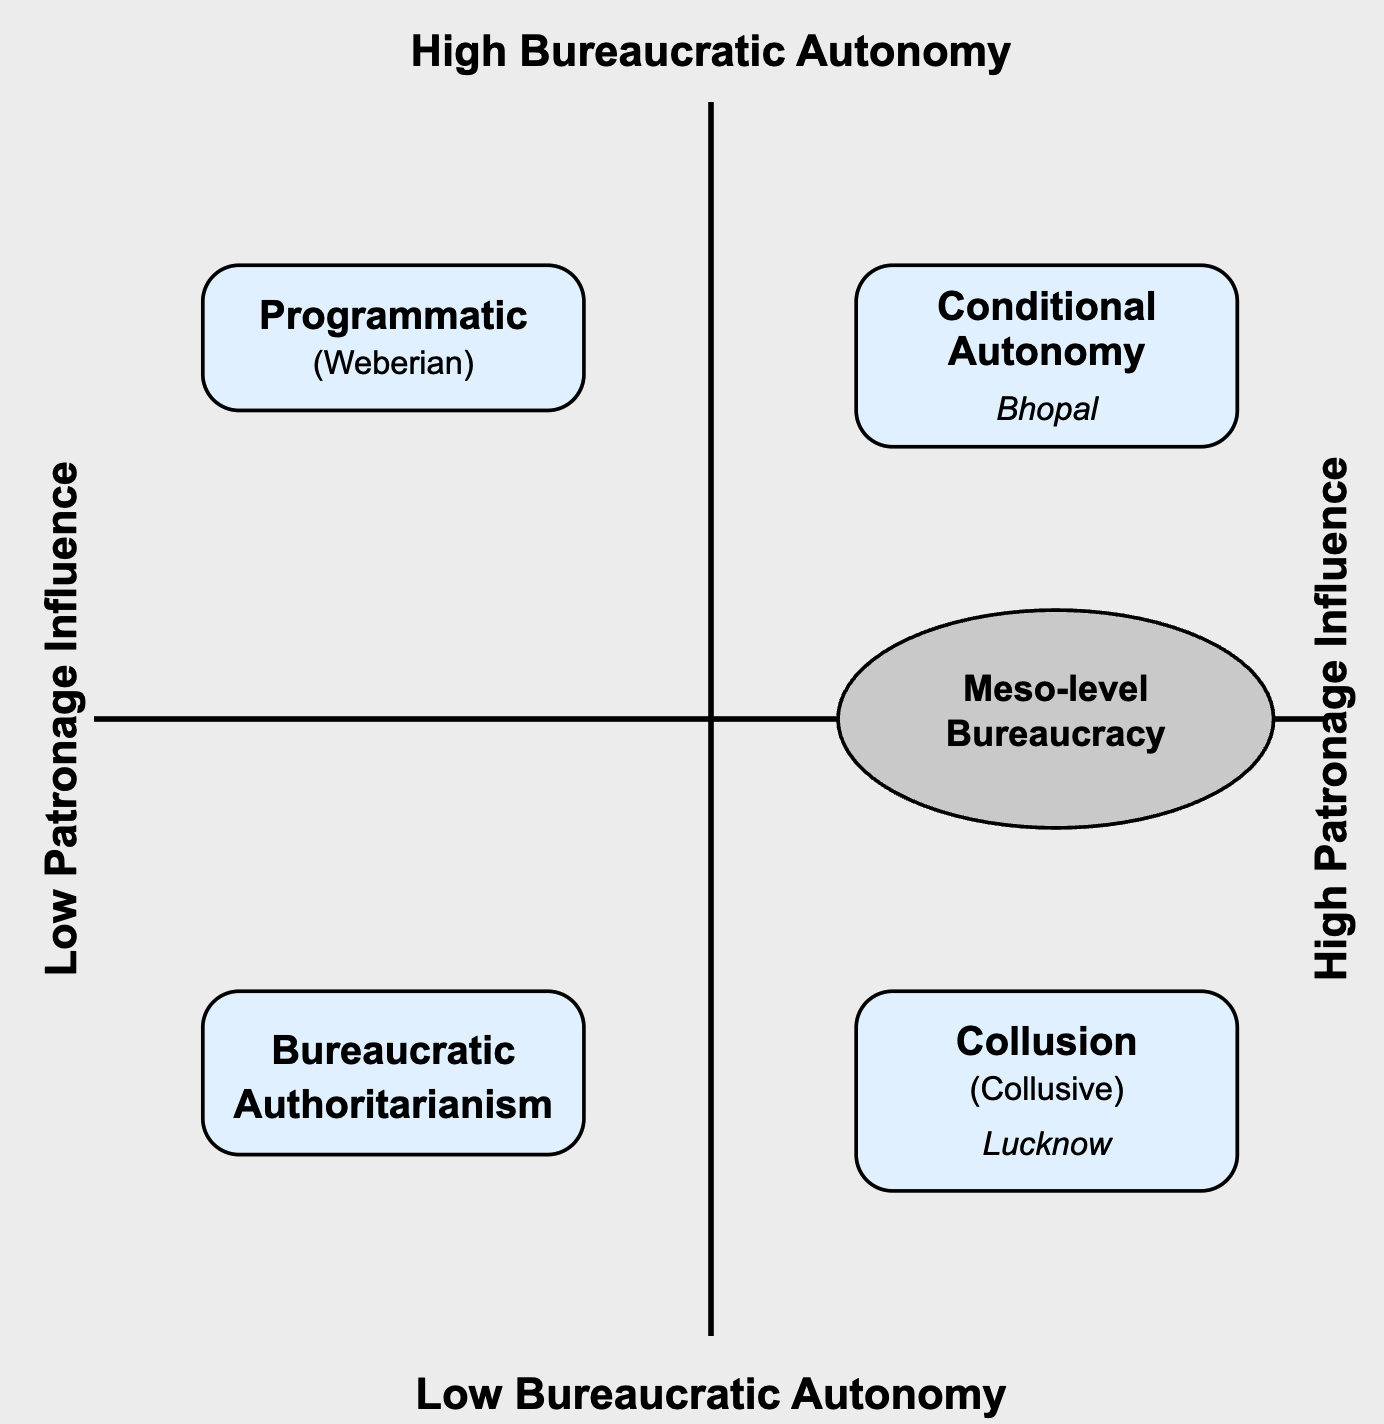
\includegraphics[width=0.85\textwidth]{figures/01_1.png} % Replace with your filename
    \caption{Your descriptive caption goes here.}
    \label{fig:your-label}
\end{figure}

\begin{itemize}
    \item Top-left (Programmatic-Weberian): The idealized model of high bureaucratic autonomy and
low patronage influence, where professional civil servants implement universal policies.
 \itemTop-right (Conditional Autonomy): The critical intermediate zone of high bureaucratic
autonomy despite high patronage influence. Here, bureaucrats maintain professional discretion
while navigating political pressures. Bhopal exemplifies this mode.
 \itemBottom-left (Bureaucratic Authoritarianism): The relatively rare configuration of low
bureaucratic autonomy with low patronage influence, representing systems lacking both
direction and agency.
 \item Bottom-right (Collusion): The trap of low bureaucratic autonomy with high patronage
influence, where bureaucrats
\end{itemize}

The framework's key insight centers on the oval in the patronage half of the matrix—the empirical reality
for most developing countries. From this position, meso-level bureaucracy faces a crucial fork: either
ascend toward conditional autonomy or descend into collusion. This choice determines not just
governance quality but whether certain essential public goods can be delivered at all.

\begin{figure}[H]
    \centering
    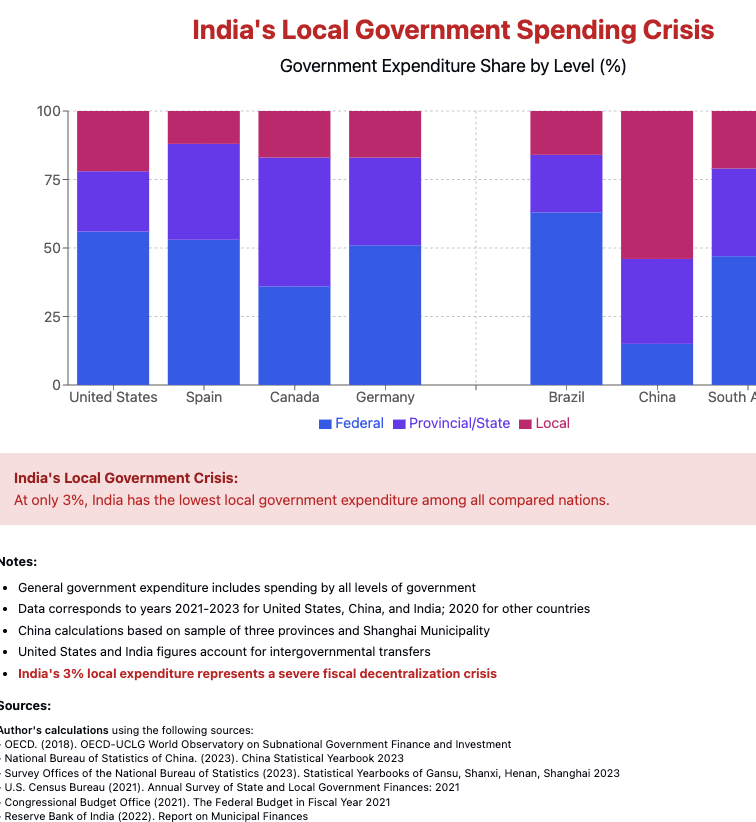
\includegraphics[width=0.85\textwidth]{figures/01-01.png} % Replace with your filename
    \caption{Figure 1: Relationship between bureaucracy and Politics}
    \label{fig:your-label}
\end{figure}

Figure 2 presents the empirical distribution of countries using V-Dem data for 2023\footnote{The horizontal axis measures political patronage influence (using reversed 'v2psprlnks' where higher
values indicate more patronage), while the vertical axis measures bureaucratic autonomy (using
'v2clrspct' where higher values indicate greater autonomy). The quadrants are delineated by thresholds
at x=0 for patronage and y=0 for autonomy, corresponding to our theoretical typology}. The horizontal
axis measures political patronage influence, while the vertical axis measures bureaucratic autonomy.
The quadrants are delineated by thresholds at x=0 for patronage and y=0 for autonomy, corresponding
to our theoretical typology. In this graph:

\begin{itemize}
    \item Top-left quadrant: Countries like Germany, Switzerland, and the United States cluster here,
representing established programmatic-Weberian systems with low patronage and high
bureaucratic autonomy.
\item Top-left quadrant: Countries like Germany, Switzerland, and the United States cluster here,
representing established programmatic-Weberian systems with low patronage and high
bureaucratic autonomy.
\item Top-right quadrant: Countries like Singapore and post-conflict states occupy this space,
demonstrating that bureaucratic autonomy can coexist with patronage politics.
\item  Bottom-left quadrant: Relatively few countries occupy this space of low patronage and low
autonomy, suggesting this is an unstable or transitional configuration.
\item Bottom-right quadrant: Most developing countries cluster here, including India, Indonesia,
Ghana, and Afghanistan, confirming that collusive governance dominates in patronage-heavy
environments.

\end{itemize}

This clustering reveals that for most of the developing world, the critical governance challenge isn't
eliminating patronage—politically impossible in the short term—but preserving or building bureaucratic
autonomy within these constraints. The vertical spread on the right side demonstrates that bureaucratic
autonomy under patronage conditions is an important variable. This positioning fundamentally reframes
our understanding of governance possibilities. Rather than viewing patronage as uniformly detrimental,
the framework reveals how bureaucratic autonomy determines whether patronage contexts produce
functional governance or collusive dysfunction. The key distinction isn't the presence of patronage which is a given in most developing contexts—but whether bureaucracy maintains sufficient autonomy
to move above or below the Y axis in the two graphs that is does the bureaucracy get conditional
autonomy to innovate or it gets instrumentalized to maintain the status quo. That in essence is the point
of this dissertation.
Understanding these distinct governance modes—particularly the crucial distinction between
conditional autonomy and collusion—sets the stage for examining their concrete implications: how
these different bureaucrat-politician relationships affect the actual delivery of public goods and services.


\section{Public Goods Delivery: Why Conditional Autonomy Excels with Non-Targetable Goods}

The theoretical distinction between conditional autonomy and collusion becomes most consequential when examining public goods delivery, particularly through the critical divide between \textbf{targetable} and \textbf{non-targetable} goods that reveals why bureaucratic autonomy matters most for essential infrastructure and networked services (Table~\ref{tab:targetable-non-targetable}).

Targetable goods are those that can be organized within a district or jurisdiction without requiring network-wide coordination. Examples include ward-level road works, neighborhood solid waste collection, and installation of tubewells or handpumps. These services exhibit spatial divisibility and require action from only one or two state actors. Given their tightly bounded costs, timelines, and benefits, politicians can promise resurfaced lanes or improved waste collection within a single electoral cycle. Engineering staff can execute these works without extensive coordination. Crucially, politicians maintain complete discretion over where and when services are delivered, allowing strategic allocation for political gain.

In contrast, \textbf{non-targetable goods}—including piped water supply, sewerage-linked household toilets, and grid electricity upgrades—require network integrity, synchronized investment, and coordination among water boards, sewerage agencies, power utilities, and various levels of government. With gestation periods extending over years and benefits diffusing across boundaries, accountability becomes difficult to assign. Most importantly, the technical characteristics of these goods eliminate political discretion in distribution, making them less attractive for patronage-driven politics unless strong higher-tier leadership ensures coordination.

This asymmetry explains why jurisdictions frequently demonstrate rapid, visible improvements in road infrastructure and tubewells, while core network services like piped water remain underdeveloped. Politicians favor targetable goods because they offer maximum discretion, while non-targetable goods require durable coalitions and commitments that survive electoral transitions.

\begin{table}[H]
\centering
\caption{Targetable vs Non-Targetable Goods}
\label{tab:targetable-non-targetable}
\small
\begin{tabularx}{\textwidth}{|l|X|X|}
\hline
\textbf{Aspect} & \textbf{Targetable Goods} (roads, neighborhood trash, tubewells, handpumps) & \textbf{Non-Targetable Goods} (piped water, sewer-linked toilets, grid electricity) \\
\hline
Spatial divisibility & High – can be delivered ward-by-ward or even lane-by-lane & Low – networks must function city-wide to be viable \\
\hline
Administrative actors & One or two municipal departments; minimal external coordination & Multiple utilities and regulators; cross-departmental synchronization essential \\
\hline
Gestation period & Short (weeks–months) & Long (years; often multi-phase) \\
\hline
Political “deliverability” & Easy to showcase within one term; ideal for ward funds and patronage & Benefits arrive after the next election; harder to claim credit \\
\hline
Equity risk & High spatial inequality—favored streets improve first & Lower once built, but slow roll-out leaves many areas unserved for long periods \\
\hline
Key governance task & Prevent pork-barrel bias and ensure minimum standards everywhere & Create durable, cross-agency coalitions and financing mechanisms to finish the network \\
\hline
\end{tabularx}
\end{table}

For simple, readily targetable services—including intermittent water standposts, streetlights, or periodic waste removal—both conditional autonomy and collusion can facilitate some form of delivery. Under collusion, these goods may be distributed as political favors (\textit{localized patronage}), with politicians exercising full discretion. Under conditional autonomy, the same services achieve more even and reliable distribution, approaching \textit{universalized delivery}, though not achieving full universality (Figure~\ref{fig:universalism-model}).

However, for complex, networked infrastructure—such as piped water systems or sewerage networks—the distinction between conditional autonomy and collusion becomes critical. The technical demands of these goods eliminate the flexibility that makes targetable goods politically attractive. Conditional autonomy enables \textbf{precarious universalism}: broad, but not perfect, coverage that remains vulnerable yet substantially superior to the fragmented outcomes of collusive governance.

Without professional norms, strategic investments, and partial insulation from political pressures, complex infrastructure projects are prone to collapse. In collusive systems, non-targetable services experience \textbf{complete fragmentation}, precluding the possibility of stable, citywide solutions and reducing service delivery to patchy, politically motivated interventions rather than coherent development.

\begin{figure}[H]
    \centering
    \includegraphics[width=0.7\textwidth]{universalism_model.png} % <-- Replace with your figure
    \caption{Impact of Conditional Autonomy vs Collusion on Public Goods Delivery}
    \label{fig:universalism-model}
\end{figure}


Politicians operating within patronage systems actively resist non-targetable goods precisely because their technical characteristics eliminate the discretion essential for patronage politics. These goods cannot be selectively directed to reward supporters due to their inherent network properties. Unlike targetable goods, which allow politicians to choose which ward receives road improvements or better waste collection, non-targetable goods operate on an all-or-nothing basis, removing political discretion.

Under collusion, these characteristics lead to \textbf{complete fragmentation}. Politicians perceive no electoral advantage in championing non-targetable goods they cannot selectively distribute, while instrumentalized bureaucrats lack both autonomy and incentive to pursue them. The result is disconnected water projects and patchwork private systems, shaped by political calculations rather than technical coherence.

Conversely, conditional autonomy enables \textbf{incremental universalism}—the significant though imperfect expansion of networked services despite patronage pressures.
The differential performance between governance modes reveals why meso-level bureaucratic autonomy proves indispensable for delivering non-targetable goods:

\begin{itemize}
    \item \textbf{Technical complexity demands professional management:} Politicians typically lack the expertise to design integrated systems. Only bureaucrats with engineering training can navigate the technical requirements of networked infrastructure.
    
    \item \textbf{Long time horizons require institutional continuity:} While politicians face electoral cycles, meso-level bureaucrats provide the institutional memory essential for multi-year projects.
    
    \item \textbf{System integrity requires protection from diversion:} Non-targetable goods fail when funds are misappropriated or redirected. Conditional autonomy creates barriers against political interference.
    
    \item \textbf{Low political discretion creates bureaucratic opportunity:} Politicians often overlook non-targetable goods precisely because they offer no discretion in distribution and limited electoral payoff, inadvertently creating space for bureaucratic initiative.
\end{itemize}

The implications are profound. Reform efforts in weak institutional environments should focus precisely where conditional autonomy yields maximum impact: non-targetable, networked infrastructure. Rather than pursuing comprehensive institutional transformation, strategic interventions that protect meso-level bureaucrats managing water, sewage, or transportation systems can produce disproportionate welfare gains.

This targeted approach acknowledges political realities while exploiting blind spots in the patronage system. Politicians may resist granting broad bureaucratic autonomy but often overlook technical domains with limited patronage value. By empowering meso-level bureaucrats in these specific areas, reformers can achieve significant improvements without directly confronting the political foundations of patronage.

\section{Conditional Autonomy: A Relational and Negotiated Equilibrium}

The empirical evidence necessitates a fundamental reconceptualization of governance dynamics. Conditional autonomy represents neither a transitional phase nor a hybrid anomaly, but rather a stable, self-reinforcing equilibrium operating within patronage-dominated contexts. This equilibrium possesses its own internal logic, performance profile, and sustainability mechanisms that demand theoretical elaboration.

To restate, this dissertation conceptualizes conditional autonomy as simultaneously relational, evolving, and negotiated between politicians and bureaucrats at the meso level. Its relational nature emerges from ongoing interactions—a dynamic balance of power and mutual expectations—rather than formal institutional rules alone. Its evolutionary character manifests in the capacity to strengthen or erode as political and performance dynamics shift. Its negotiated aspect operates not through singular formal agreements but through implicit understandings, tacit accords, and occasionally explicit pacts that delineate bureaucratic discretion. Essentially, conditional autonomy grants bureaucrats limited independent authority contingent upon specific conditions: delivering measurable results, avoiding open defiance of core political interests, and demonstrating value to political patrons. This equilibrium occupies a middle zone between two theoretical extremes. It exhibits neither the full Weberian autonomy of bureaucracies impervious to political interference nor the complete capture characteristic of politicized bureaucracies. Instead, it represents a stable arrangement where both bureaucrats and politicians find maintaining partial bureaucratic independence rational and mutually beneficial.

The equilibrium's stability derives from bidirectional accountability and mutual constraint-benefit trade-offs. Politicians in conditional autonomy regimes restrain from excessive interference in specific bureaucratic domains, recognizing the performance benefits of limited autonomy. Reciprocally, bureaucrats utilize their discretionary authority to generate outcomes reflecting positively on political leadership while remaining cognizant that autonomy remains contingent. This creates a self-enforcing dynamic: bureaucrats maintain performance to protect their autonomy, while politicians preserve bureaucratic discretion to secure political dividends through improved service delivery.

In game-theoretic terms, this represents a repeated interaction achieving cooperative equilibrium. Politicians' credible threat of reverting to patronage control disciplines bureaucratic behavior, while bureaucrats' demonstrated capacity to deliver results deters political interference. This equilibrium demonstrates fragility yet resilience—vulnerable to shocks such as leadership changes or major policy failures but persistent while both parties perceive the arrangement as superior to alternatives.

This conceptualization resonates with Evans's notion of "embedded autonomy" in developmental states, though operating in a different context. Where Evans described bureaucracies combining autonomous structures with dense societal ties, conditional autonomy combines professional integrity with embeddedness within patronage politics. The bureaucracy operates not behind insulating walls but maintains professional zones within patronage pressures.

Conditional autonomy also resolves what Geddes termed the "politician's dilemma"—the tension between exploiting state resources for immediate political gain versus building competent civil services yielding longer-term benefits. Neither extreme serves politicians' interests optimally: fully autonomous bureaucracies undermine short-term electoral needs, while completely politicized bureaucracies sacrifice developmental capacity.

The logic of conditional autonomy becomes evident when examining performance across varying task complexity levels (Figure 4).

\begin{figure}[H]
    \centering
    \includegraphics[width=0.8\textwidth]{figure4_placeholder.png}
    \caption{Governance Mode Effect on Complexity of Good}
    \label{fig:governance_complexity}
\end{figure}

Figure 4 presents three distinct performance curves:

\begin{itemize}
    \item The Patronage Mode (blue line) demonstrates high effectiveness for simple tasks but experiences a steep, linear decline as complexity increases. This reflects patronage systems' ability to distribute targetable benefits efficiently while failing catastrophically at complex, networked tasks requiring technical coordination.
    \item The Programmatic Mode (red line) exhibits relatively low effectiveness for simple tasks but maintains steady performance as complexity increases, showing a gradual decline only at higher complexity levels. This pattern reflects programmatic systems' emphasis on universal rules and procedures over discretionary distribution.
    \item Conditional Autonomy (orange/yellow line) begins with high effectiveness for simple tasks— nearly matching patronage performance—but declines more gradually than patronage as complexity increases. Critically, it maintains superior performance to both programmatic and patronage modes across the middle range of complexity, demonstrating its unique advantage for moderately complex tasks.
\end{itemize}

This performance pattern reveals why conditional autonomy represents a viable equilibrium: it combines the distributional efficiency of patronage for simple tasks with sufficient technical capacity for moderately complex challenges. While it may not match programmatic systems at extreme complexity, conditional autonomy achieves "good enough governance" precisely where most essential public services operate—in the middle range of complexity where neither pure patronage nor rigid programmatic approaches perform optimally.

The graph thus illuminates why conditional autonomy emerges and persists: it offers a pragmatic balance between political imperatives and developmental outcomes, producing sufficient benefits for both politicians and citizens to ensure self-sustainability in patronage-dominated contexts.

\subsection{How Meso-Level Bureaucrats Exercise Conditional Autonomy}

The theoretical construct of conditional autonomy finds its practical expression through four distinct yet interconnected mechanisms which though alluded earlier are given fuller attention here. These mechanisms—bureaucratic brokerage, strategic intermediation, intertemporal stabilization, and normative institutionalization—represent not merely organizational functions but fundamental transformations in how governance operates under constraints. Together, they explain how mid-level officials convert limited autonomy into disproportionate governance improvements.

\paragraph{Intermediaries within the State: The Strategic Position of Meso-level Bureaucrats}

A fundamental challenge in state capacity is coordinating activities across line departments. This isn't just abstract theory—it's the everyday reality of getting water departments to talk to sanitation departments, or education officials to coordinate with health services when school feeding programs are implemented. Traditional "silo mentality" plagues bureaucracies worldwide, with each department jealously guarding its turf, budget, and authority. Meso-level bureaucrats occupy a uniquely advantageous position as intermediaries within the state apparatus itself—inverting our usual focus on brokers and middlemen operating outside formal state structures.

Their location in the administrative hierarchy enables critical coordination that neither elites nor street-level bureaucrats can achieve: Horizontally, they bridge departmental divides without the baggage that hampers others. Unlike top brass whose interactions are limited by protocol, status consciousness, and turf protection, mid-level officials can pick up the phone and call their counterpart in another department without triggering a bureaucratic crisis. They don't need formal memoranda or committee approvals to initiate problem-solving conversations. These officials share a common bureaucratic language and professional ethos that transcends departmental boundaries, allowing them to cut through red tape when line departments need to work together.

Vertically, these officials function as crucial conduits between ground realities and policy circles. Street-level bureaucrats—the teachers, nurses, and agricultural extension workers—possess intimate knowledge of implementation challenges but lack the authority to push these insights upward. They're trapped in their daily routines, processing cases one at a time. Department secretaries and directors, meanwhile, remain removed from operational messiness, focused on high-level policy formulation and political navigation. Mid-level bureaucrats translate between these worlds—bringing field observations to headquarters while interpreting policy intentions to implementers.

A municipal commissioner might convey to the state government that a water policy isn't working because local pipes are too old, while simultaneously explaining to local engineers why compliance with new state standards matters. This dual intermediary function makes mid-level bureaucrats the connective tissue of the state machinery. Unlike the classic focus on external intermediaries who operate between state and society (the ward boss, the fixer, the NGO facilitator), these internal intermediaries work within the administrative architecture itself, reinforcing connections between departments and across hierarchical levels. When they exercise conditional autonomy, they can address coordination deficits that formal structures often fail to resolve, creating pragmatic solutions to bureaucratic fragmentation even amidst pervasive patronage pressures. This intermediary function can be formalized as a mechanism of bureaucratic brokerage, whereby meso-level officials leverage their unique structural position to bridge otherwise disconnected departments and hierarchical levels, facilitating information flows and resource coordination that formal systems often fail to achieve.

% (The remaining sections – Boundary Spanners, Memory, Stewardship – would follow in same format, verbatim. Let me know if you want the rest split or posted now.)

\paragraph{Boundary Spanners: The Interstitial Role of Mid-level Bureaucrats}

While mid-level bureaucrats function as internal intermediaries, they simultaneously operate as crucial boundary spanners at the state-society interface (Williams, 2002; Honig, 2018). This interstitial positioning constitutes their second vital contribution to state capacity in contexts of conditional autonomy.

The boundary-spanning function emerges from a practical organizational dilemma: elite bureaucrats must maintain professional distance from potentially compromising interactions. Senior officials cannot regularly engage with contractors, local power brokers, or politicians with particularistic agendas without risking their professional standing or ethical reputation. Yet these engagements remain necessary for implementing policies and programs.

Mid-level bureaucrats fill this interstitial space, engaging with external actors that higher officials cannot directly approach. This arrangement functions through a tacit division of labor. Senior bureaucrats delegate boundary-spanning responsibilities to their mid-level subordinates, who negotiate with builders, contractors, elected representatives, and other external stakeholders.

A municipal commissioner might direct a deputy to handle negotiations with a construction firm rather than conducting these discussions personally. Similarly, politicians utilize these officials as intermediaries when pursuing both programmatic and particularistic aims, recognizing their operational knowledge and implementation authority.

The interstitial position creates a dual potential: mid-level bureaucrats can leverage these relationships to enhance program effectiveness and resource mobilization, or they may be instrumentalized by political or commercial interests seeking preferential treatment. Their position is inherently ambiguous, simultaneously offering opportunities for administrative entrepreneurship and avenues for co-optation.

This intermediary function can be formalized as a mechanism of strategic intermediation, whereby mid-level bureaucrats maintain legitimate standing with multiple principals simultaneously—their bureaucratic superiors, political authorities, and external stakeholders—creating protected spaces for administrative discretion even within patronage-dominated environments.

\paragraph{Institutional Memory Carriers: The Temporal Continuity Function}

While mid-level bureaucrats serve critical spatial intermediation functions—bridging departments horizontally and hierarchical levels vertically—they simultaneously perform an essential temporal function as carriers of institutional memory (Pollitt, 2009; Schön-Quinlivan, 2011). This contributes a third vital dimension to state capacity in contexts of conditional autonomy.

This function manifests in public administration systems worldwide, where projects spanning multiple years or even decades persist despite rapid turnover at senior leadership levels. While high-level officials may rotate frequently, mid-level bureaucrats maintain project continuity through their accumulated knowledge. Their institutional memory encompasses both formal aspects (regulation details, procedural requirements) and tacit knowledge (knowing which files matter, where documents are stored, how budgetary allocations work in practice).

This memory function addresses a fundamental governance challenge in developing contexts: the high turnover of senior officials that creates institutional amnesia. In many bureaucracies, elite positions rotate frequently due to political transitions or internal promotion patterns. Street-level bureaucrats, while potentially stable in their roles, lack the systemic perspective to preserve institutional continuity. Mid-level officials bridge this temporal gap, having sufficient longevity in their positions to accumulate deep organizational knowledge while possessing enough authority to deploy this knowledge effectively.

As Weber (1978) observed in his analysis of bureaucratic expertise, effective administration depends not merely on formal rules but on the "craft knowledge" that develops through immersion in organizational processes. Bourdieu's (1990) concept of habitus further illuminates how officials embody institutional practices, developing an intuitive feel for navigating complex bureaucratic fields. Mid-level bureaucrats exemplify this embodied knowledge, having internalized both explicit procedures and implicit norms that guide administrative action.

This intermediary function can be formalized as a mechanism of intertemporal stabilization, whereby mid-level bureaucrats maintain critical organizational knowledge across leadership transitions, ensuring policy continuity despite the discontinuous nature of political and elite administrative tenures in developing contexts.

\paragraph{The Professional Stewardship Function}

Beyond their intermediary roles, meso-level bureaucrats perform a fourth critical function through their cultivation of professional stewardship within state institutions. This dimension addresses a fundamental gap in traditional administrative theory that has predominantly characterized bureaucrats through rational choice frameworks—as utility-maximizing agents driven primarily by material self-interest or career advancement.

While strategic self-interest undoubtedly shapes bureaucratic behavior, field research reveals a more complex motivational landscape among mid-level officials. Their extended tenure within specific departments—often spanning decades in a single institutional setting—creates a distinctive relationship to their organizational context that transcends purely instrumental calculations.

Unlike elite bureaucrats who frequently rotate between postings or street-level workers with limited authority to shape institutional direction, mid-level officials develop profound identification with their departments. As one district officer articulated during field interviews: "I will spend my entire career in this department. If I don't improve it now, I'll have to live with the consequences for the next 30 years." This temporal horizon fundamentally alters their decision calculus, transforming short-term challenges into long-term investments in institutional effectiveness.

This professional stewardship emerges most strongly under conditions of partial autonomy, where bureaucrats retain enough discretion to experience meaningful agency while facing resource constraints that necessitate creative problem-solving. They cultivate what DiMaggio and Powell (1983) describe as "normative isomorphism"—professional standards that become internalized and reproduced across organizational contexts, creating resilience against patronage pressures.

This function can be formalized as a mechanism of normative institutionalization, whereby mid-level bureaucrats with extended departmental tenures develop and sustain professional values that persist beyond individual officeholders, creating institutional resilience that enables cumulative improvements in state capacity even within imperfect governance environments.


These four mechanisms—bureaucratic brokerage, strategic intermediation, intertemporal stabilization, and normative institutionalization—collectively illuminate how mid-level bureaucrats operate as the connective tissue of state capacity. By bridging structural, relational, temporal, and normative dimensions of governance, they create integration where fragmentation would otherwise prevail.

The combined effect is transformative: rather than bureaucracy that passively follows orders or actively serves private interests, we observe proactive, self-regulating innovation within political boundaries. The conditionality of autonomy ensures responsiveness, while the autonomy enables application of skill, knowledge, and coordination capacity to public problems.

This framework reconceptualizes the "missing middle" not as a theoretical gap but as a pivotal arena where state capacity is actively constructed through distributed agency. Mid-level officials navigate between formal mandates and informal realities, establishing horizontal connections, spanning external boundaries, maintaining institutional memory, and cultivating professional norms—practical statecraft that conventional theories overlook.

By illuminating these mechanisms, we gain both analytical leverage for understanding subnational variation and practical insights into fostering incremental improvements in state capacity, even within challenging institutional environments.

\section{A Model of Bureaucratic Authority in Weak Local States: The Divergent Paths of Governance}

To formalize the theoretical relationships outlined above, we develop a comprehensive model of bureaucratic authority pathways in weak local states, demonstrating how initial conditions and path dependencies produce divergent governance outcomes.

\begin{figure}[H]
    \centering
    \includegraphics[width=0.85\textwidth]{figure5_model.png} % Replace with actual filename
    \caption{How does conditional autonomy operate}
    \label{fig:figure5_model}
\end{figure}

Figure 5 presents a comprehensive model of bureaucratic authority pathways in weak local states, illustrating how initial political choices cascade into distinct governance equilibria. The model begins with a fundamental precondition: the existence of a weak local state characterized by limited institutional capacity and strong patronage networks.

The critical juncture occurs when political elites face pressure for reforms, either from citizens demanding better services or external actors promoting governance improvements. This pressure triggers a bidirectional decision point: whether political elites will grant autonomy to meso-level bureaucrats. The model reveals two distinct pathways, each with self-reinforcing dynamics that lead to divergent long-term outcomes.

When political elites deny bureaucratic autonomy, the system defaults to bureaucratic collusion. In this pathway, bureaucrats become fully instrumentalized by political patrons, leading to poor service delivery characterized by both targetable goods distributed as patronage and fragmented, non-viable attempts at complex infrastructure. The outcome crystallizes as localized patronage, where public resources serve narrow political interests rather than broad developmental goals.

When political elites opt to grant conditional autonomy, however, a more complex pathway emerges.

This choice triggers a cascade of positive developments: bureaucrats gain space to coordinate activities, build technical capacity, and address complex challenges that pure patronage systems cannot manage. The resulting improved service delivery—particularly in non-targetable, networked goods—generates a crucial feedback loop. Citizens and external actors provide political support for these improvements, which reinforces the political rationality of maintaining bureaucratic autonomy.

The model's key insight lies in the self-reinforcing nature of both pathways. Under collusion, poor performance legitimizes further political interference, creating a downward spiral. Under conditional autonomy, improved performance generates political rewards that sustain bureaucratic discretion, creating a virtuous cycle. This explains why jurisdictions with identical formal institutions can achieve dramatically different outcomes: initial political choices about bureaucratic autonomy set in motion path-dependent processes that become increasingly difficult to reverse.

The model also illuminates why conditional autonomy proves particularly crucial for delivering non-targetable goods. Only through sustained technical coordination and professional discretion can bureaucrats overcome the inherent challenges of networked infrastructure—challenges that patronage systems systematically fail to address. This theoretical framework thus provides both explanatory power for observed variations and practical guidance for reform efforts in weak institutional environments.

\subsection*{Summary}

This section accomplished two critical objectives. First, it identified significant blind spots in existing scholarship regarding variation in service delivery within patronage settings. The literature's focus on national-level institutions, abstract structural factors, and binary conceptions of state capacity has systematically overlooked the crucial role of meso-level bureaucratic dynamics in explaining subnational governance variation.

Second, it established a new theoretical framework to resolve this puzzle. The core argument posits that low-capacity, patronage-dominated polities perform unevenly because governance outcomes depend fundamentally on the interaction between political incentives and bureaucratic autonomy. When meso-level officials retain conditional autonomy—limited but real discretion within patronage systems—they can mobilize professional norms and inter-departmental authority to coordinate complex, citywide networks (water, sewerage, power) that individual politicians cannot parcel out as favors. This bureaucratic coordination improves service coverage and reliability, creating positive feedback loops that gradually institutionalize higher-capacity governance.

Conversely, where such autonomy is absent and officials operate in fully collusive relationships with politicians, service delivery fragments into localized patronage enclaves, trapping the state in low-performance equilibria.

The section also provided measurement strategies, a causal model, and specified the characteristics of meso-level officers and conditions under which they can innovate.

The next section transitions to examining the empirical context from which these theoretical insights emerge—Indian cities. It first establishes what Indian cities represent as cases for theory development, demonstrating their value for state capacity research and comparative politics more broadly. It then presents detailed case studies of Bhopal and Lucknow, providing empirical validation for the theoretical model developed here.

The next section moves to understanding the context from which these theory has been driven – Indian cities. First, it provides you with an overview asking – what is Indian city a case of? And how can it be a site for theory generation for state capacity in particular and comparative politics in general. It then discusses the cases I study, Bhopal and Lucknow – showing the validity or proof of concept of this model.

\part{Part B}

\section{What is the Indian City a Case of: Indian Cities and the Paradox of State Capacity}

\subsection{Fragmented and Uneven State Capacity in Urban India}

Indian cities powerfully illustrate the fragmented and uneven nature of state capacity in the Global South. In development theory, scholars often note that state authority does not extend uniformly across territory or social groups. Guillermo O'Donnell's notion of "brown areas," for instance, pointed to enclaves within democracies where the rule of law and public institutions are weak.

This spatial and institutional fragmentation creates precisely the conditions where conditional autonomy emerges as a governance mode—mid-level bureaucrats must navigate multiple, overlapping authorities through negotiated practices rather than clear lines of command. This empirical reality makes Indian cities ideal cases for examining how the meso-level bureaucrats theorized in Section 1 navigate governance challenges. What conventional theoretical lenses dismiss as dysfunction instead creates the interstitial spaces that make conditional autonomy not just possible but necessary for effective governance.

Indian urban centers exemplify this pattern of institutional fragmentation in particularly stark terms. Within a single metropolis, pockets of high-capacity governance coexist with areas where the state's reach is tenuous and public services are deficient. This unevenness is not merely a rural-urban divide, but an intra-urban reality—a city of enclaves and exclusions rather than a monolithic unit of governance. In short, Indian cities encapsulate a broader paradox: a state that is impressively present in some domains and absent in others, challenging conventional models that treat state capacity as a homogenous national trait.

Crucially, this fragmented state capacity is not a static accident of history—it is produced and reproduced by governance structures. Indian cities operate within a federal system where local governments have formally defined powers, yet practically constrained autonomy. The result is often "islands" of capacity—effective delivery of certain services or in certain locales—surrounded by vacuums or overlaps elsewhere. Such outcomes reflect more than just uneven investment; they point to how the machinery of the state itself is fragmented, with multiple agencies and levels of government struggling (or failing) to coordinate. Indian cities thus personify the idea that state capacity is not monolithic—it varies widely within countries and even within cities, defying any singular characterization of "strong" or "weak" state. This reality provides fertile ground to test and refine theories of state capacity and development that have often been drawn from more unified national experiences.



\subsection{Overlapping Governance and Public Goods Delivery}

A key reason for the patchwork performance of Indian cities is their complex governance structure – a maze of overlapping jurisdictions and divided authority. Unlike cities in many other democracies, Indian municipalities do not enjoy exclusive control over urban affairs. Instead, critical functions are shared (and sometimes contested) among multiple institutions: city corporations, state government departments, public sector boards (for water, transport, housing, etc.), and even special development authorities. This multiplicity leads to ambiguous responsibility. Who is accountable for providing water, managing traffic, or maintaining drains in a city? Often it is not one entity but several, each with a piece of the task. The consequence is duplication in some areas and vacuum in others – a recipe for inefficient and unequal public goods delivery. Four structural features characterize urban governance in India and shape public goods provision:


\subsubsection*{Multiplicity of Agencies}

Indian cities operate under fragmented governance structures, with state- created parastatals functioning parallel to elected municipal bodies. These specialized agencies—water boards, development authorities, slum clearance boards—report directly to state governments, bypassing local democratic oversight. As illustrated in Figures 1-2 this fragmentation manifests starkly in spatial planning arrangements across major metropolitan regions. In Mumbai, 13 sub-regional planning authorities operate alongside the Municipal Corporation. Hyderabad's planning authority absorbed four erstwhile agencies yet still operates eight plans prepared by multiple authorities which remain in force. In Bangalore this number is 8 and Chennai even with a relatively simpler structure, divides planning between the development authorities master plan and a staggering 57 high-growth areas requiring detailed development plans (Table 3).

What appears as an organizational arrangement is fundamentally a political problem of sovereignty. These parastatals were ostensibly created to enhance technical capacity, but in practice have "usurped functions and revenues that ought to have been the domain of cities," undermining what Heller calls the "binding of the state" to citizens through participatory processes. Most critically, control over urban planning and land use—the foundation of meaningful urban governance—remains centralized in 80\% of states/UTs. This institutional arrangement creates precisely the governance vacuum where conditional autonomy becomes significant: mid-level bureaucrats must navigate between formal constraints and local realities, mediating between state directives and community needs.

Without territorial authority over land, municipal governments cannot function as strategic actors, instead becoming spaces where bureaucrats exercise conditional discretion within narrowly defined parameters—often creating the very governance gaps that require bureaucratic entrepreneurship to address. This institutional fragmentation directly illustrates the governance context theorized in Section 2, where meso-level bureaucrats must employ bureaucratic brokerage to coordinate across siloed agencies and departments. Together, these features create a governance environment where mid-level officials must navigate both horizontal fragmentation across agencies and vertical disconnection from democratic accountability.


\begin{figure}[H]
    \centering
    \includegraphics[width=0.8\textwidth]{figures/mumbai_planning.png}
    \caption{Multiple Spatial Planning Arrangements in Mumbai Metropolitan Region. The map shows 13 sub-regional planning authorities operating alongside the Municipal Corporation, illustrating the extreme fragmentation of governance. Source: Regional Plan for Mumbai Metropolitan Region (1996--2011), MMRDA.}
    \label{fig:mumbai_planning}
\end{figure}

\begin{figure}[H]
    \centering
    \includegraphics[width=0.8\textwidth]{figures/hyderabad_planning.png}
    \caption{Multiple Spatial Planning Arrangements in Hyderabad Metropolitan Region. Despite HMDA's formation by merging four erstwhile planning authorities, multiple planning regimes remain in force. Source: CPR Analysis.}
    \label{fig:hyderabad_planning}
\end{figure}


\subsubsection*{Administrative Dominance: When Bureaucracy Eclipses Democracy}

Urban governance across India exhibits a consistent pattern: turnout in municipal elections stays stubbornly low even as citizens energetically “work the state” through personal networks, political brokers, and direct bureaucratic appeals. In this context, appointed officials regularly eclipse elected representatives, and the ubiquitous commissioner system has become less a neutral administrative device than a political arrangement in which bureaucratic hierarchies substitute for democratic channels. Municipal Commissioners—typically drawn from the elite Indian Administrative Service (IAS)— control staff appointments, budgets, and day-to-day service delivery with only minimal local oversight. Yet my calculations show that these IAS commissioners serve in any given city for a median tenure of
 


just 16 months, whereas mid-career state-cadre (“meso-level”) officers in Madhya Pradesh (MP) and Uttar Pradesh (UP) remain in comparable municipal posts far longer (18 months for UP and 24 months for MP). It is precisely these longer-serving, locally embedded administrators who form the empirical core of this study: their extended tenures furnish the organizational memory and discretionary space that make—or break—urban governance outcomes (Figure 6).

Meanwhile, elected Mayors serve largely ceremonial functions despite being the formal face of city government. This creates what might be called a ``sovereignty gap'' in urban governance. While formal democratic processes exist—elections are held, councils meet, debates occur—the substantive authority to implement decisions flows through bureaucratic rather than democratic channels. The constitutional amendment of 1992 that formally recognized urban local bodies (city governments) attempted to bridge this gap, but its implementation paradoxically reinforced administrative dominance by giving state governments discretion over the actual powers devolved to cities.

The governance arrangement where bureaucratic hierarchies—at elite, meso, and frontline levels— exercise greater authority than elected bodies creates precisely the conditions this dissertation examines —neither fully autonomous (as they must respond to state-level political pressures) nor completely captured (as they retain significant discretionary authority over implementation). Unlike classic governance models where bureaucrats simply implement political decisions, officials at all levels must actively interpret, adapt, and negotiate formal directives to accomplish basic functions. This distributed bureaucratic authority, particularly at the meso-level, becomes critical for understanding how cities actually function despite their institutional constraints.

The consequences run deeper than institutional design. This governance model shapes the very nature of urban politics. Elected councilors, unable to directly control administration, evolve into specialized intermediaries who help constituents navigate bureaucratic processes rather than crafting policy. The bureaucracy, nominally apolitical, becomes the de facto center of political dealmaking and resource allocation. This inversion creates governance spaces where informal negotiations between bureaucrats and special interests often matter more than formal democratic deliberations.

The result is a governance ecosystem where democratic energy exists but lacks institutional channels for effective expression. Urban residents experience government primarily through bureaucratic encounters rather than democratic representation. This arrangement persistently undermines the development of vibrant local democracy while simultaneously requiring bureaucratic innovation to overcome the coordination failures it creates—a self-reinforcing cycle that maintains administrative dominance while necessitating the very discretionary bureaucratic practices it supposedly constrains.

\section{Fiscal Emasculation: The Financial Incapacitation of Urban Governance}

City governments in India face crippling fiscal constraints that fundamentally undermine their governance capacity. This financial powerlessness represents not merely a technical deficiency but a structural governance arrangement where municipalities possess formal responsibilities without corresponding financial tools—what scholars call ``unfunded mandates'' (Ahluwalia, 2019).

The fiscal marginalization is quantitatively severe: municipal governments control only 1-2\% of public expenditure, compared to 20-35\% in other major federal democracies (Mathur, 2021). Figure 7 demonstrates this stark disparity—while local governments in countries like the United States, Spain, and Brazil control between 20-45\% of government expenditure, India's local governments manage a mere 3\%, the lowest among all compared nations. This constraint operates through multiple institutional mechanisms. This constraint operates through multiple institutional mechanisms: constitutional provisions for predictable resource transfers remain unimplemented by most states; taxation authority is severely curtailed; and borrowing requires explicit state approval, effectively foreclosing municipal access to capital markets.

\begin{figure}[htbp]
\centering
\caption{Share of Local Government Expenditure Across Countries}
\label{fig:fiscal_constraint}
% Insert your figure here
\end{figure}

Three consequences directly flow from this fiscal architecture. First, cities depend on discretionary, politically-mediated transfers rather than stable, rules-based funding. Second, financial management deteriorates as municipal corporations routinely miss budget targets by 40-60\%, creating a governance environment where planning becomes performative rather than operational. Third, accountability mechanisms collapse as responsibility and authority disconnect—elected officials face citizen demands they lack resources to address.

Their resulting practices—informal resource mobilization, negotiated rule enforcement, contingent service delivery—represent not corruption but strategic adaptation to systemic constraints. The comparative perspective reveals this is not inevitable: South African municipalities receive constitutionally guaranteed revenue shares, while Brazilian cities control significant local tax bases (Shah \& Shah, 2020).

Without addressing this deliberate fiscal incapacitation, the formal trappings of urban democracy— elections, councils, citizen participation—will continue to mask the substantive reality: cities that cannot govern effectively because they cannot finance even their most basic mandates. This financial powerlessness exists within and reinforces a broader governance framework that systematically concentrates resources at state and national levels, leaving cities perpetually under-resourced despite their growing economic importance and population.

\section{Residual Urbanism: Rural Primacy \& The Systematic Marginalization of Urban India}

India's governance exhibits a profound rural bias that manifests in three distinct ways. First, restrictive classification criteria systematically undercount urban populations. While official statistics place urbanization at 31\%, my earlier work has shown that applying internationally comparable definitions would reveal that India is approximately 40\% urban (Joshi \& Pradhan, 2018) The peculiar category of ``census towns''—settlements that meet demographic criteria for urban status yet remain administratively rural—exemplifies this statistical distortion\footnote{India employs one of the most restrictive urban definitions globally. Urban areas are divided into Statutory Towns (with elected urban local bodies) and Census Towns (meeting three criteria: population $\geq$5,000, density $\geq$400 persons/km², and $\geq$75\% male workforce in non-farm sector). Despite qualifying as urban, Census Towns remain administratively rural, governed by rural local bodies.}

Second, institutional incentives drive deliberate misclassification. State governments strategically maintain rural classifications because rural status confers greater financial resources with fewer administrative constraints. The most striking example occurred in 2004 when Tamil Nadu—then India's most urbanized state—reclassified over five hundred urban areas as rural to obtain more funds from the Union government (Sivaramakrishnan, 2013). This represents not statistical error but rational response to a governance framework that privileges rural development.

Third, and most fundamentally, Indian policy conceives urban space as merely residual defined not by what it is but by what it is not (rural). Unlike the ``urban bias'' literature pioneered by Michael Lipton (1977) that positions cities as privileged in developing countries, India's reality presents the inverse: a governance system that systematically favors rural interests while neglecting spaces where economic and demographic growth concentrate most intensely. While Varshney's (1993) critique demonstrated that Lipton's original formulation neglected key mediating factors—particularly democratic institutions providing rural populations electoral leverage, technological changes like the Green Revolution enhancing rural political power, and identity politics fragmenting simple rural-urban coalitions—the Indian case nonetheless represents a clear inversion of the urban bias thesis.\footnote{Varshney's analysis emphasizes that democratic institutions fundamentally alter the political landscape by giving rural populations electoral leverage absent in Lipton's original framework. The nature of political regimes, technological transformations, and identity-based mobilization all mediate the expression of sectoral interests in ways that complicate any simple model of structural bias.}

This rural primacy creates profound governance consequences that extend beyond simple resource allocation. Most critically, it generates a systemic urban representation deficit in legislative bodies. Due to the prolonged freeze on constituency delimitation based on 1971 Census data, urban areas now suffer severe under-representation. Bengaluru, despite accounting for 14\% of Karnataka's population, holds only 10-12\% of legislative seats; Pune's urban areas receive only 2.7\% of Maharashtra's assembly seats; and nationally, only 15\% of Lok Sabha constituencies can be classified as majority urban despite approximately 40\% of the population living in urban areas.\footnote{This representation deficit violates the democratic principle of `one person, one vote, one value' due to vastly different constituency sizes. The freeze on seat reallocation after 1971, extended through successive constitutional amendments, creates a political imbalance where urban legislators represent significantly larger populations than their rural counterparts. Combined with weak fiscal autonomy and heavy dependence on intergovernmental transfers, this political under-representation exacerbates urban governance challenges.} This structural under-representation compounds fiscal weaknesses, as Urban Local Bodies depend on central transfers rather than robust own-source revenues, creating gaps in infrastructure and service delivery precisely where population pressure is most acute. The result is a governance ecosystem that systematically undermines urban capacity while simultaneously requiring adaptive strategies from diverse actors—bureaucrats, elected officials, civil society organizations, and citizens—who must navigate this marginalization through the complex mechanisms of negotiation and intermediation this dissertation examines.

These four structural features collectively create what might be termed an `accountability vacuum' in urban governance. The principal-agent relationship fundamental to democratic accountability—where voters (principals) hold elected officials (agents) responsible for service delivery—becomes fundamentally distorted. Municipal councilors lack authority over bureaucrats who report to state capitals; service-providing agencies answer to multiple masters; and financing flows through discretionary rather than rules-based channels, leaving elected representatives unable to fulfill their democratic mandates.

This accountability fragmentation creates precisely the governance space where conditional autonomy emerges as a necessary adaptation. Within these institutional constraints, mid-level bureaucrats must deploy the four mechanisms theorized in Section 2: bureaucratic brokerage to coordinate across fragmented agencies, strategic intermediation to interpret ambiguous mandates, intertemporal stabilization to maintain policy continuity amid political flux, and normative institutionalization to establish informal rules that compensate for formal gaps. Their effectiveness depends not on following rigid hierarchies but on navigating relationships with multiple stakeholders—state officials, elected representatives, community organizations, and private interests.

The resulting governance model explains both the persistent failures and unexpected successes observed in Indian cities. Services deteriorate where bureaucrats cannot bridge these accountability gaps, creating neighborhoods that fall through institutional cracks. Conversely, effective service delivery emerges where entrepreneurial officials successfully navigate fragmented structures through conditional discretion—creating `islands' of capacity within otherwise dysfunctional systems. Understanding these dynamics requires moving beyond institutional design to examine how bureaucratic agency operates within and around formal constraints, precisely the contribution this dissertation makes to theories of state capacity in constrained environments.

\section{Bureaucratic Autonomy versus Political Accountability}

The governance configuration of Indian cities raises a classic question in development theory: how does one strike the right balance between bureaucratic autonomy and political accountability, particularly in contexts of severe fiscal constraints, fragmented legal authority, and financial dependence. The Indian case suggests that this balance is especially elusive in urban contexts, and it complicates prevailing models like the principal--agent framework or Peter Evans's notion of ``embedded autonomy.''

Bureaucratic autonomy—the insulation of civil servants from politicization—is traditionally seen as a virtue of capable states. In Indian cities, however, we often see the downsides of excessive autonomy and of too little autonomy, coexisting uneasily. The autonomy of city bureaucrats in India exemplifies our conditional autonomy framework from Section 2. These officials operate with partial independence from local electoral pressures, shielded by their appointment through state/national civil services. This creates precisely the type of negotiated equilibrium we theorized, where bureaucrats maintain professional discretion within politically defined boundaries, neither fully insulated nor completely captured. This could prevent short-termism or clientelist distribution at the local level. Yet, this autonomy from local accountability can also morph into detachment and unresponsiveness. A bureaucrat who rotates into a city for a couple of years might feel answerable primarily to superiors in the state capital rather than to the city's populace. If the Commissioner prioritizes state government directives or personal career considerations (e.g. avoiding controversy), local needs may be sidelined. In this sense, bureaucratic autonomy in Indian cities often means autonomy from the public, which can undermine the very purpose of public service.

On the other hand, bureaucrats in Indian cities are not wholly autonomous in a Weberian sense – their functioning is deeply enmeshed in political currents, only the currents come from above and outside the city. State-level politicians (chief ministers, ministers, legislators) routinely intervene in city matters, including in personnel decisions. Transfers of municipal officers at the behest of politicians are commonplace, sending a clear signal that stepping on powerful toes can be career-ending. There are numerous instances of municipal commissioners or ward engineers being shunted out because their actions (like removing illegal encroachments or enforcing rules impartially) displeased an influential politician or interest group. This dynamic fits a principal-agent logic, but with a twist: the bureaucrat becomes an agent to multiple principals – not just the lawful political principal (the city's elected body) but also to higher-level political actors. The result is a tenuous bureaucracy, adept at surviving through accommodation. The famed ``steel frame'' of the All-India Services in practice bends to political winds in the urban context. Autonomy, in the Evans sense, is compromised when bureaucrats must anticipate political reactions to every move. But unlike a clean principal-agent hierarchy, here the lines of authority are blurred: city bureaucrats navigate a dual accountability – upward to state leaders, and nominally downward to local citizens, often pleasing the former at the expense of the latter.

This scenario complicates principal--agent models. Classic theory envisions elected officials (principals) setting goals and monitoring bureaucrats (agents) to ensure implementation aligns with voters' interests. In Indian cities, who is the principal? The local councillor has formal authority but limited power; the state minister has actual clout but is not directly accountable to the city's voters for municipal services. The agent (bureaucracy) thus juggles instructions from multiple principals with differing priorities. Moreover, the agents themselves have some autonomy to pursue their own agendas or biases, especially given the opacity of who is in charge. Such a system can breed accountability confusion and even perverse incentives – for example, a municipal officer might delay action on a local issue until a state politician intervenes, thus securing favor with the latter. The principal-agent framework can be stretched to accommodate multiple principals, but Indian cities suggest we might need more networked or polycentric models of governance to describe reality. Authority is dispersed and negotiated rather than neatly delegated.

Another theoretical lens is provided by street-level bureaucracy, Michael Lipsky's idea that front-line public servants effectively make policy through their discretionary actions. Indian cities present textbook conditions for street-level bureaucracy to flourish. This discretionary power operates within a context of severe human resource deficits. Indian municipalities are dramatically understaffed compared to international counterparts—Bengaluru employs only 317 staff per 100,000 residents and Delhi about 601, compared to nearly 3,000 in London and 6,000 in New York. As Figure 8 illustrates, India's local governments have the lowest share of public employees among comparable emerging economies, with state governments absorbing the vast majority of administrative capacity. This staffing crisis is exacerbated by vacancy rates often exceeding 30-40\%, alongside significant skill gaps in specialized areas like urban planning, transport engineering, and financial management. With limited professional training and state governments controlling key appointments, municipal bureaucrats operate in an environment of both scarcity and constraint. Within this capacity vacuum, the few available front-line workers (clerks, engineers, inspectors, police constables) end up exercising enormous discretion in allocating public goods. Because high-level policies and directives often do not align or are infeasible in the face of resource constraints, street-level officials become de facto policymakers.

\begin{figure}[htbp]
\centering
\caption{Distribution of Public Employees Across Government Levels}
\label{fig:employees_distribution}
% Insert your figure here
\end{figure}

For example, a ration shop officer in a city may decide which families receive scarce subsidized foodgrains, or a junior engineer may informally prioritize repairing the water line in one neighborhood over another. In Mumbai's water distribution system, valve operators (chabiwalas) exemplify this phenomenon with particular clarity—these operators literally hold the keys to the city's water supply, determining through their daily valve adjustments which neighborhoods receive water, when they receive it, and with what pressure (Anand, 2017). Their decisions transform physical infrastructure into a mechanism of social stratification, creating what Anand terms ``hydraulic citizenship''—a form of belonging defined by one's ability to secure reliable water access. These ground-level decisions reflect not only official guidelines but also personal judgments, prejudices, and pressures. In a context where formal accountability is weak, street-level officials are susceptible to influence by local power brokers or their own rent-seeking interests. The phenomenon of ``speed money'' – small bribes to get things done – exemplifies how street-level bureaucrats can gatekeep services, effectively ruling in practice over who gets what.

Thus, while Indian cities suffer from high-level fragmentation, it is often the street-level functionaries who stitch together some semblance of order, albeit through improvised, ad-hoc adjustments rather than systematic policy. This confirms Lipsky's insight that the real policies delivered to citizens are often decided on the street, not in official plans – but it also shows how such discretion, in the absence of accountability, can perpetuate uneven service and even arbitrariness.

In sum, the Indian urban experience pushes us to refine ideas of bureaucratic autonomy and principal-agent relations. It suggests that autonomy must be paired with embeddedness in accountability structures – a point that recent research underscores. For instance, a study of Indian districts found that bureaucrats who hail from the area they administer (hence more embedded locally) can improve public goods provision, but only when local accountability (media, literacy, civic engagement) is strong; otherwise, local ties may simply enable capture by elites (Bhavnani and Li 2018). This resonates in cities: when municipal bureaucrats work in isolation from citizen voice (no strong accountability mechanisms like transparent feedback or empowered councillors), their autonomy veers into unresponsiveness; yet if they were fully subject to local politics without institutional safeguards, service delivery could devolve into parochial patronage. Indian cities thus exemplify the challenges of achieving balanced bureaucratic autonomy – that is, independence from partisan exploitation without detachment from public accountability.

\section{The Role of Clientelism and Informal Mediation}

Given the structural constraints and the often-impersonal stance of the formal state apparatus, how do ordinary urban citizens in India secure the public goods and services they need? The answer, in many cases, lies in informal networks, patronage, and clientelism filling the breach. When rules and institutions do not guarantee basic necessities, people turn to what Partha Chatterjee famously described as ``political society'' – the realm where citizens mobilize not just as rights-bearing individuals, but as members of patron-client networks, trading political support for material benefits.

Operating within this context of limited formal power and a politically fragmented urban society— where caste, religion, and class significantly shape political mobilization and voter allegiances— councilors adopt patronage politics as a rational strategy for political survival. Unable to effect broad policy changes, they leverage their limited, informal influence over the distribution of targetable non-networked goods like fresh tar on a patch of road, trash management, or lamp posts controlled at the local level. Within this constrained governance environment, a complex ecosystem of brokers—middlemen, touts, and fixers—has embedded itself into public service delivery systems. As recent research demonstrates, these brokers act as gatekeepers who ``block or expedite access to public services based on payment of a fee'' in cities like Delhi.

This reframing of clientelism as rational adaptation rather than mere corruption aligns with significant theoretical developments in political science and institutional analysis. Recent scholarship by Jennifer Gandhi, Adam Przeworski, and Beatriz Magaloni demonstrates how seemingly clientelistic practices often emerge as rational responses to specific institutional constraints rather than from corrupt motivations. Similarly, Rebecca Weitz-Shapiro's research on Argentina shows that clientelism persists precisely because it solves concrete governance problems in environments where formal mechanisms fail. Urban data from India for 14 cities substantiates this perspective: corporators receiving predominantly positive evaluations (60\% viewed as serving all constituents) suggests citizens themselves distinguish between corrupt rent-seeking and legitimate, if constrained, service provision.\footnote{Source: Authors' calculation based on Citizenship, Inequality, and Urban Governance (CIUG) Project, Brown University} Importantly, this ``constituency service clientelism'' operating through elected representatives differs significantly from more problematic forms involving illegal kickbacks or vote buying. By recognizing clientelism as a rational institutional adaptation—albeit one with significant governance costs—we gain deeper insight into why these practices persist despite decades of reform efforts. The persistence of such arrangements reflects not primarily moral failings but structural constraints that make alternative governance modes practically infeasible for both representatives and citizens.

Our survey data across 14 Indian cities provides empirical evidence that refines our understanding of how this system operates in practice. Contrary to theoretical expectations that emphasize state-level legislators or informal middlemen, citizens overwhelmingly identify municipal corporators as their primary channel for accessing public services. As Figure 9 demonstrates, in smaller cities, corporators remain the primary channel for accessing services with 51\% of residents identifying them as their first point of contact, while in large metropolitan areas this drops to 25\%. Even more surprising, citizens maintain largely positive views of these relationships—60\% believe corporators serve all constituents equitably rather than particular communities (13\%) or themselves (18\%). This suggests that what scholars often frame as clientelism is experienced by many citizens as legitimate constituency service.

\begin{figure}[htbp]
\centering
\caption{Who do you think is most important to deliver services to you?}
\label{fig:service_delivery}
% Insert your figure here
\end{figure}

Indian cities are frequently portrayed as arenas of vibrant electoral competition, yet this narrative masks two important realities. First, voter turnout in municipal elections consistently lags behind state and national contests. As Figure Y illustrates, municipal elections average only 49\% turnout compared to 62\% in parliamentary and 59\% in state elections, reflecting what Dasgupta (2015) terms ``the local democracy gap.'' Second, beneath the formal electoral processes lies a hustle for direct access: access to water, housing, electricity, sanitation, jobs, and permits through personal intervention rather than systemic improvements.

\begin{figure}[htbp]
\centering
\caption{The Local Democracy Gap: Average Voter Turnout by Election Type}
\label{fig:voter_turnout}
% Insert your figure here
\end{figure}

These intermediation practices operate within an institutional environment that severely constrains corporators' formal authority. Shadowing corporators in Lucknow revealed the limitations of their role. As one candidly expressed, ``We are firefighters, trash pickers, and drain openers. That is our role (hum aag bhujane wale hai, kuda uthane wale hai, naali khulwane wale hai).''\footnote{Quote from a city councilor in Lucknow, 2022} This statement vividly illustrates how local politicians are forced to assume administrative functions typically handled by bureaucrats. In the absence of substantive policy-making authority, corporators rely on patronage not primarily as a corruption strategy but as their only viable means of exercising influence. The structural constraints within which they operate—approximately 31\% of India's 4,766 municipal governments were effectively inactive as of 2023—transform even formal representatives into brokers within a dysfunctional system\footnote{Authors calculation using Local Self Government Directory and Comptroller and Auditor Generals Report}.

These personalized interventions represent classic examples of clientelistic exchanges – the voter gets a problem solved as a favor, and the politician hopes to get loyalty (or at least credit) in return. For marginalized citizens who lack formal paperwork or find themselves ignored by the system, a patron who can bend the rules becomes a lifeline. Research by Auerbach and Thachil (2018) reveals that urban brokers, unlike their rural counterparts, provide personalized and highly targeted services such as dispute resolution and assistance with documentation. Clientelism, in this sense, functions as a coping mechanism that compensates for the state's uneven performance – a way to navigate a fragmented system by leveraging personal influence rather than universal rights.

The consequences of this system for effective urban governance are profound. It undermines strategic, city-wide planning and leads to inequitable and inefficient service delivery, frequently prioritizing politically connected groups or areas while neglecting systemic improvements. Accountability becomes diffused, shifting from formal performance standards to informal, often opaque, transactional relationships, which can obscure responsibility and potentially foster corruption. Meaningful citizen participation is often curtailed, reduced to making particularistic demands on councilors rather than engaging in broader policy debates or holding the ULB accountable for overall city performance.

However, the clientelistic model has profound limitations that become increasingly evident in India's big cities. First, it is inherently particularistic—only some people benefit, often at the expense of others. In an urban constituency of say 300,000 people, even the most energetic representative can directly assist only a fraction. As research shows, politicians inevitably end up solving problems for some constituents while alienating others, even among their core supporters.

Second, this system does not scale well as cities grow. As Simon Chauchard notes, the increasing size of urban electorates and the complexity of needs make quid-pro-quo arrangements hard to sustain – there are simply too many constituents and issues for patronage to cover, and urban voters are often more heterogeneous and less tied to traditional patron-client bonds than rural voters. This scaling problem is reflected in our survey data, which shows that positive perceptions of corporators decline significantly from small cities (72\%) to large metropolises (55\%). Modern cities thus dilute the effectiveness of old-style machine politics; while clientelism is still present, it struggles to cope with the breadth of urban service deficits.

The institutional dysfunction that necessitates these clientelistic relationships creates a suboptimal equilibrium where no party truly benefits. When formal governance mechanisms break down—councils are dissolved, scheduled meetings fail to occur, and administrative processes stall—citizens have no choice but to reach out to councillors as their first line of action. These councillors, in turn, become overwhelmed by individual requests they lack the institutional capacity to address systematically. The resulting arrangement traps both citizens and representatives in a perpetual cycle of ad-hoc problem-solving that diverts attention from the structural reforms needed for effective urban governance.

Additionally, clientelism and informal mediation can undermine institutional development. If everyone must go through a ``broker'' to get basic services, there is less public pressure to improve the system for all. In fact, politicians themselves can become invested in the status quo of dysfunction, since it validates their role as indispensable fixers. This dynamic is captured in the phrase: ``The rich have peers, the poor have patrons.'' Wealthier or more educated city dwellers can often navigate bureaucracy through formal or professional networks (or purchase private alternatives), whereas the poor depend on patronage. Such patterns entrench inequalities of access. They also blur the lines between the formal state and informal practices: many bureaucrats expect political recommendations or informal payoffs to expedite work, effectively entwining clientelism with everyday administration.

These findings complement and extend Chatterjee's conceptualization of political society. While Chatterjee correctly identifies how marginalized groups must negotiate with the state through political rather than purely rights-based channels, our data reveals the central role of formal elected representatives within these negotiations. Rather than operating primarily through community-based mobilization, urban residents frequently engage directly with corporators as individuals seeking services. This direct engagement with corporators, combined with their positive perception despite limited formal powers, suggests a more complex relationship between citizens and the state than is captured in standard clientelism frameworks.

At the same time, one should not ignore the adaptive ingenuity in these arrangements. Urban residents form associations, slum federations, or use local media to amplify their issues, essentially trying to collectivize bargaining with the state when possible, not just individualize it. There are instances where community-led efforts got the municipality to install street lights or toilets, effectively compelling the state to respond without traditional patronage. Such civic initiatives interact in complex ways with clientelism – sometimes they supplant it, other times they themselves seek the patronage of a sympathetic official.

In summary, informal governance – through clientelist ties, brokers, and on-the-ground improvisation – is a double-edged sword in Indian cities: it provides relief and navigation in a fragmented system, but it also reinforces fragmentation by working around systemic solutions. Any analysis of state capacity and public goods in these cities must therefore grapple with this symbiosis of formal structures and informal strategies, recognizing that what appears as patronage often represents the only viable channel through which citizens can access basic services in a governance system that structurally constrains democratic mechanisms.

\section{Fragmented but Functioning: Rethinking State Capacity in Indian Cities}

While the previous sections establish that Indian cities exhibit profound deficiencies by most conventional measures of ``state capacity''—fragmented authority, weak fiscal autonomy, administrative undermanning, and structural constraints—a puzzling reality persists: these same cities continue to function and even thrive in crucial domains. Basic services, though unevenly distributed, reach millions of residents; urban economies generate significant growth; and innovative policy approaches regularly emerge from this seemingly dysfunctional landscape. This paradox—governance systems that appear broken yet remain operational—raises a fundamental question: How do Indian urban systems sustain themselves amid such institutional disorder? The conventional metrics of state capacity, with their Weberian ideals of bureaucratic coherence and hierarchical clarity, fail to explain this resilience.

\subsection{The Empirical Paradox: Progress Against All Odds}

What makes this theoretical puzzle empirically compelling is that Indian cities have demonstrated measurable improvements in service delivery over decades despite their institutional constraints. National Sample Survey data since 1992 reveals steady gains in access to basic services even under stringently defined parameters: piped tap water within premises and safe sanitation (toilets connected to sewers, septic tanks, or ventilated pit latrines meeting UNICEF standards) (Figure 11). This empirical reality fundamentally challenges purely pessimistic narratives of governance failure that dominate much of urban studies literature.

\begin{figure}[htbp]
\centering
\caption{Public goods in Indian cities over three decades. Authors Calculation}
\label{fig:public_goods}
% Insert your figure here
\end{figure}

I argue that state capacity in the Indian urban context is not a static attribute that municipalities either possess or lack, but rather an emergent property of complex, adaptive systems. It manifests through ongoing processes of negotiation, contestation, and co-production among diverse actors working within and around institutional constraints. What formal institutional analyses might dismiss as dysfunction— overlapping jurisdictions, informal arrangements, and ad hoc problem-solving (jugaad)—often represents creative adaptation to structural limitations. The very improvisational quality of urban governance, with its negotiated practices and institutional bricolage, makes Indian cities critical sites for reconceptualizing state capacity in the Global South.

By engaging with this messy reality rather than measuring cities against idealized governance models imported from Northern contexts, we uncover a contingent, improvised form of state capacity that paradoxically enables cities to function despite their apparent institutional weaknesses. This perspective helps explain why, despite their fiscal and administrative fragility, complex institutional overlaps, and chronic under-resourcing, local state remain vital arenas of public service delivery, political contestation, and institutional innovation. That makes the paradox all the more intriguing: Indian cities are deeply fragmented yet somehow functional, historically neglected yet increasingly vital. This section therefore asks, provocatively, what ``capacity'' really means in such a context.

\subsection{Historical Neglect and the Late Turn to Urban Reforms}

To fully appreciate the current fragility of the cities—and their paradoxical resilience—one must confront the historical neglect that shaped them. The Indian state effectively abandoned urban governance for the first fifty-odd years after Independence, treating cities as administrative afterthoughts rather than engines of development. Unlike rural development (which saw nationwide programs like community development blocks in the 1950s, Integrated Rural Development in the 1970s, etc.), urban development remained a residual category in national planning. The dominant policy narrative cast urbanization as a byproduct of development, even a necessary evil to be managed, rather than a transformative process to be nurtured.

Two critical junctures mark the belated emergence of urban governance from this residual status. First, the 74th Constitutional Amendment Act of 1992 provided legal recognition to urban local bodies, though without commensurate fiscal or administrative capacity. This half-hearted constitutional acknowledgment created the formal shell of local urban democracy without the substantive powers that might give it life. The second, perhaps more consequential juncture came over a decade later when India launched its first national urban renewal mission. The Jawaharlal Nehru National Urban Renewal Mission (JNNURM), unveiled in December 2005, marked a dramatic shift—the single largest urban development initiative in India's history up to that point. JNNURM explicitly linked central government funding to reform conditions, requiring cities to implement property tax reforms, e-governance, master plans, and other changes to receive infrastructure grants.

Yet this late awakening came after decades of systemic neglect. By 2004, India was already approximately 28\% urban with hundreds of millions living in towns and cities; yet the institutional scaffolding for managing this urban population remained skeletal at best. Even today, combined public spending on urban development by states and Centre hovers around a mere 3\% of GDP, grotesquely disproportionate to what India's urban population ratio would suggest is needed. By contrast, China's decades of high urban investment fueled much smoother service provision, highlighting how this historical neglect has materially shaped India's current urban crisis.

The period since 2004 has witnessed a parade of federal schemes (AMRUT for water supply, Smart Cities Mission, Swachh Bharat for sanitation, and others), each attempting to improve aspects of urban governance and service delivery. These have certainly infused resources and some innovations, yet the scheme-driven approach underscores how the urban local state remains not organically empowered but rather pulled up by external incentives—a dependent rather than autonomous actor in its own development.

This historical trajectory explains why Indian urban governance is as fragmented and frail as it is— because robust local institutions were never a priority until crises emerged. The local state we see today is a product of path dependency: decades of treating cities as administrative wards of states rather than self-governing entities. This historical lens reveals that any evaluation of performance must be tempered by the recognition of this late start—cities have been expected to do more with much less preparation time than other sectors. Yet importantly, it also reveals that improvements, however modest, have occurred despite this historical handicap—suggesting a form of resilience and adaptive capacity that traditional state capacity frameworks struggle to explain.

\subsection{The Local State in Action: Legal Ambiguity and Bureaucratic Agency}

One reason the local state in India functions in a negotiated way is the nature of laws and rules governing it. Urban governance operates in a zone where formal laws are often vague, outdated, or internally contradictory, necessitating interpretation and norm-setting by administrators. The Madhya Pradesh Municipalities Act provides a revealing window into this reality: it creates a formal obligation (provide water) but simultaneously negates any enforceable accountability (no citizen can sue for non-supply). The upshot is that the real obligation is determined by norms, not by the text of law.

This legal ambiguity, rather than merely creating dysfunction, paradoxically creates space for mezo-level bureaucrats to exercise critical discretion. In Bhopal, for example, municipal officials have leveraged this legal ambiguity to extend water delivery to nearly all informal settlements despite no explicit mandate to serve unauthorized areas. The municipal official's interpretation that ``adequate provision'' means doing the best possible with available resources becomes more important than strict legal interpretations. This is governance by bureaucratic agency, not by legislative clarity.

In effect, local governance in India is often government by precedent and practice. Officials learn ``how things are usually done'' from their seniors, and those practices can matter more than what the Acts and rules say. There is considerable room for interpretive maneuver. For instance, if a municipal act says the city ``may'' establish ward committees for citizen participation, whether this happens or not depends on the state's and city's political will. In most states these provisions lay dormant (hence the lack of functional ward committees in many cities), creating a norm of low citizen consultation, despite the 74th Amendment's intent.

Conversely, where reformist bureaucrats have interpreted laws more aggressively, they have occasionally expanded the scope of city action. In Pune, for instance, municipal officials pioneered participatory budgeting practices by creatively interpreting legal provisions on citizen consultation, establishing a model that subsequently spread to other cities. Similarly, Indore's transformation into one of India's cleanest cities occurred not through any revolutionary legal mandate but through bureaucrats leveraging existing provisions while building interdepartmental coordination around solid waste management. These examples illustrate how bureaucratic norms and practice can reshape governance outcomes despite legal ambiguities.

The law thus sends mixed signals to the bureaucracy: ``Do your best, but there's no penalty if you don't succeed.'' In such an environment, what guides action is not legal compulsion but administrative and political culture. If the city or state leadership prioritizes universal water coverage, they will drive the bureaucracy to use its discretionary power to expand services. If not, the clause remains just lofty language. This understanding is a kind of unwritten policy— a tacit agreement that aligns with neither a full laissez-faire approach (they do attempt to provide services) nor a rights-based approach (they stop short of aiming for universality). It is, fundamentally, governance by negotiated settlements: settlements in both the literal sense (informal settlements get water through negotiated means) and the figurative sense (different arms of the state and community ``settling'' for intermediate solutions).

\subsection{Engaging the Local State: From Dysfunction to Transformation}

If fragmented and underpowered city agencies are part of the problem, could they also be part of the solution? It might seem counterintuitive—many policy-makers have bypassed municipal bodies precisely because they appear ineffective. Yet there is growing recognition that sustainable improvement in urban governance requires working with and strengthening local institutions rather than perpetually circumventing them. In other words, the path to transforming city governance runs through the messy local state, not around it.

Odisha's Jaga Mission offers a compelling case. This state-led initiative set out to grant land tenure rights to slum dwellers across cities and upgrade those settlements with basic infrastructure. What makes Jaga Mission particularly remarkable is that it emerged in Odisha—a state traditionally categorized as ``low capacity'' by most development metrics—yet achieved substantial success. Although conceived at the state level, it was implemented largely through existing local governance structures. Municipal officers, ward councilors, and community volunteers in each city were mobilized to survey slum households, identify beneficiaries, and oversee improvements. The state provided the policy framework, funds, and oversight, but on-ground execution relied on city-level actors. The results were remarkable: according to official government sources and independent reports over 2,00,000 families have received secure land titles, and hundreds of slum communities saw tangible upgrades in roads, lighting, sanitation, and more. By empowering slum residents and involving municipal institutions directly in delivering tenure and services, the mission not only improved living conditions but also built confidence and capacity within urban local bodies of a supposedly ``low capacity'' state.

Studies of Basic Services for Urban Poor (BSUP) projects under JNNURM in Chennai and Ahmedabad reveal similar complexities. Coelho, Mahadevia, and Williams (2022) note how ``Chennai's state-led BSUP projects represent a concerted effort to deliver structured housing to the urban poor,'' while Ahmedabad's initiatives ``offer a more flexible model, allowing for incremental upgrades that align with the needs of residents.'' Despite the ``persistent challenge of 'dis-location,' where the relocation of low-income households to peripheral areas disrupts livelihoods and social networks,'' these initiatives demonstrated how urban missions could catalyze meaningful improvements when implemented through local institutions.

The dominant strategy in urban development has become clear: bypass the local state entirely. National programs create parallel structures—special purpose vehicles, state corporations, mission directorates— that sidestep municipal bodies altogether. While this delivers quicker results initially, it reinforces the very weaknesses it seeks to avoid.

The national urban missions reveal this tension perfectly. JNNURM and Smart Cities Mission pumped resources into cities, but local state capacity and priorities determined actual outcomes. Delhi built flyovers for its middle-class constituencies. Mumbai expanded water infrastructure across all neighborhoods, including slums. Bhopal strengthened administrative capacity through management information systems. Lucknow failed to spend funds effectively, concentrating limited investments in elite areas while ignoring wider needs. Despite uniform guidelines and funding, these cities produced radically different results—confirming that local state capacity remains the critical variable.

These missions brought new dynamics to urban governance. International and domestic consulting firms now provide ``private expertise'' at multiple levels, creating what scholars term ``Consultancy Urbanism.'' Dashboard-driven implementation prioritizes metrics over substantive change. Smart Cities abandoned JNNURM's reform agenda entirely, favoring discrete projects instead. Yet these programs created openings for reform that deserve attention. Their limitations—excessive reliance on parastatal agencies, consultant-driven approaches, metric-focused implementation—cannot obscure their significance for understanding how change emerges within constrained institutions.

By not studying these experiences, we miss crucial insights into urban transformation. The local state, though bypassed, remains the essential mediator between national ambitions and urban realities.

\subsection{Rethinking State Capacity: Insights from Indian Cities}

Examining Indian cities as a category forces a fundamental rethinking of dominant models of state capacity, governance, and development. These urban cases defy any simple classification of the state as either capable or failing—instead, they reveal a state that is heterogeneous, internally segmented, and often internally contradictory. This has several profound implications for theory:

\begin{enumerate}
\item \textbf{State Capacity as a Local Variable:} Traditional discussions of state capacity (fiscal capacity, administrative capacity, etc.) often take a country-wide view, or at best distinguish between regions. Indian cities show that capacity can vary not just regionally but organizationally— different arms of the state within the same locality have very different levels of effectiveness. One neighborhood might have reliable electricity (perhaps because a well-run state electricity board manages it), while trash goes uncollected (because the municipal solid waste department is under-resourced and nobody coordinates a solution). Thus, rather than speaking of ``the Indian state'' as having a certain capacity, we see a mosaic of capacities. This underlines the need for more fine-grained theories that look at sub-state units and inter-organizational relations.

\item \textbf{Beyond Principal-Agent: Toward Network Governance Models:} The messy reality of politician--bureaucrat interactions in cities suggests that simple principal-agent models are inadequate. Instead of a linear chain of accountability, Indian urban governance is better seen as a web of relationships—a network governance or multilevel governance system where local and higher-level actors continually negotiate power. This resonates with the idea of polycentric governance (often discussed in the context of metropolitan regions), where overlapping authorities must coordinate (or compete). Indian cities teach us that we should model governance not just as a hierarchy but as a negotiated order. The concept of embedded autonomy itself might be reinterpreted here: perhaps what's needed is an ``embeddedness'' not only in social groups (as Evans meant) but embeddedness across state institutions—for example, city officials embedded in local communities and connected to higher administrative echelons, serving as bridges.

\item \textbf{Democracy and Bureaucracy Reconsidered:} Indian cities challenge the notion that democratic decentralization automatically improves governance. Decentralization theory would suggest that bringing government closer to the people (through elected city bodies) should enhance accountability and service delivery. The Indian case shows that partial decentralization— without real devolution of power and resources—can lead to disillusionment and confusion. It is a cautionary tale that institutions matter more than labels: having a municipal council is not enough if that council cannot command the bureaucracy or finances needed to act. Conversely, the Indian urban experience also suggests that bureaucratic centralization has limits—a top-down approach that marginalizes local knowledge tends to misfire. We see this in the mixed results of one-size-fits-all national urban schemes that ``assumed a level of uniformity that doesn't exist'' across cities.

\item \textbf{The Hybrid State – Formal and Informal Synergy:} Perhaps one of the most original insights from Indian cities is how the formal and informal elements of governance intertwine to produce outcomes. Neither the Weberian bureaucracy model nor pure patron-client model alone fully captures the process; what we see is a hybrid state at work. For example, a formal government program might rely on community volunteers or political intermediaries to actually reach slum populations, essentially blending bureaucratic provision with informal social networks. This is not wholly accounted for in classic models of bureaucratic rationality or clientelism, which often treat informal practices as a deviation. In Indian cities, informality is part and parcel of governance. Recognizing this pushes theorists to move beyond binary thinking (legal/illegal, state/society) toward frameworks that accept a continuum.
\end{enumerate}

These insights extend beyond the Indian context to inform comparative theory-building on state capacity in developing democracies. By moving beyond national-level analyses to examine subnational variation through the lens of conditional autonomy, this framework offers analytical leverage for understanding governance outcomes across diverse political systems characterized by institutional hybridity and contested authority. Similar patterns of fragmented authority, fiscal constraints, and bureaucratic adaptation likely characterize urban governance across much of the Global South, suggesting broader applicability of the conditional autonomy framework developed here.

In making these arguments, Indian cities are not presented as merely failing cases or aberrations. Rather, they are instructive cases that prompt theory-building. They compel us to ask: What does ``state capacity'' really mean when capacity is distributed among different agencies? How do accountability mechanisms function when authority is diffuse? How can equitable public goods be provided in a system that leans on inequitable patronage? The answers gleaned from Indian urban contexts can help reconceptualize state capacity in the Global South as something less about a singular strong vs weak state, and more about the configuration of institutions and relationships that produce developmental outcomes. In other words, Indian cities help shift the discourse from ``Is the state capable?'' to ``Which state institutions are capable, in concert or conflict with which others, and under what conditions?'' – a far richer question.

\section{Conclusion: Opening the Black Box of Urban State Capacity}

Indian cities present a seeming paradox: on the one hand, we see institutional weakness—fragmented authority, low staffing, poor finances, ambiguous laws—and on the other, we find that cities still somehow deliver incremental improvements and maintain a livable order for millions. This chapter has argued that the resolution of this paradox lies in understanding state capacity as an improvised, negotiated practice. The local state in India is not a well-oiled machine, but neither is it a broken engine beyond repair. It is more akin to a jerry-rigged device, patched together and working in unorthodox ways.

Most scholarly analyses of the urban Global South have three tendencies that fundamentally limit our understanding of state capacity: they either focus exclusively on high-level politics (Aijaz, 2008; Kohli, 1987; Kundu, 2003), concentrate on grassroots mobilization and people's movements (Baviskar, 2003; Benjamin, 2000; Shaw, 2007), or reduce everything to neoliberal capital flows (Benjamin, 2007; Ghertner, 2011; Kundu, 2011). As Benjamin (2007) and others have argued, ``new centers of economic, political, and discursive power are emerging in Indian cities as powerful economic and social groups maneuver to achieve their objectives''—yet this neoliberal analytical frame too often obscures the agency and improvisation happening within state institutions themselves.

These dominant approaches neglect the crucial role of the local state bureaucracy where change actually happens—the officials who lay the pipes, build the sewers, and establish waste collection networks. By failing to open this ``black box'' of state functioning, we miss how improvised capacity gets built and incremental change occurs even in constrained circumstances. This dissertation fills this gap by developing a theoretical framework centered on conditional autonomy and meso-level bureaucrats, contributing to comparative politics in three significant ways...he three classic agents of urban change— bureaucracy, politics, and civil society—are all present in Indian cities, yet we have systematically neglected to study how they interact within and through local state institutions.

This perspective carries an important implication: engaging with the urban state is crucial precisely because it is imperfect. If we seek to improve service delivery, reduce inequality, or make cities more sustainable, we cannot bypass city governments and hope for lasting change. Projects that circumvent local institutions (for example, parallel private utilities or ad-hoc task forces) may provide temporary relief but are hard to sustain or scale. In contrast, working through the local state—frustrating though it may be—can lead to institutional learning and transformation. When reformers confront the bottlenecks and push for changes from within (simplifying rules, digitizing systems), they convert bottlenecks into new capacity.

In a broader sense, examining the local state in Indian cities sheds light on state capacity in the Global South. It challenges the binary view of states as either capable or failed. Indian cities show a state that is weak-but-working—a bundle of contradictions where dysfunction and functionality coexist. Infrastructure may be crumbling in parts, yet municipal elections are fiercely contested, indicating faith in the idea of city governance. Bureaucrats may be harried and under-resourced, yet they act as pivotal change-makers when windows of opportunity open. The urban state is both vilified for its incompetence and relied upon for every basic need—truly both a bottleneck and an enabler.

Thus, the dissertation's central claim is intentionally provocative: if meaningful urban transformation is happening at all in India, it is because of the local state, not in spite of it. This runs against a grain of thinking that often credits external actors (private sector, civil society, higher-level governments) for any success and blames the local state for failures. We have seen that external impetus matters (as with national missions), but it ultimately channels through the city institutions. By critically analyzing both the flaws and the potential of urban local bodies, we gain a more nuanced understanding of state capacity. Indian cities teach us that state capacity is often improvised—made on the fly through coalitions of actors, negotiated rules, and creative use of discretion. That is why cities function, even if unevenly.

This perspective provides a new lens for comparative analysis across the Global South. The conditional autonomy framework developed here offers analytical leverage beyond the Indian context, potentially illuminating governance dynamics in diverse settings where formal institutional weakness coexists with pockets of effectiveness. By focusing on how meso-level bureaucrats navigate constraints rather than simply documenting those constraints, this approach contributes to a more agency-centered understanding of governance that can inform both scholarly analysis and practical reforms across developing democracies.






\section{Bhopal and Lucknow: Similar Institutions, Radical Outcomes}

Having established how conditional autonomy emerges within India's fragmented urban governance structure, we now turn to examining the empirical case studies that illuminate these theoretical propositions.

\textbf{{Scope and Argument in Brief}}

The argument in this dissertation is that the key to understanding change in low capacity, patronage setting lies in the relationship between politics and bureaucracy.
The governance framework identifies four modes based on political incentives (programmatic vs. patronage) and bureaucratic autonomy (autonomous vs. instrumentalized):
\begin{itemize}
  \item \textbf{Programmatic:} Autonomous bureaucracy + programmatic politics = high performance
  \item \textbf{Collusion:} Instrumentalized bureaucracy + patronage politics = governance failure
  \item \textbf{Conditional Autonomy:} Autonomous bureaucracy + patronage politics = negotiated effectiveness
  \item \textbf{Bureaucratic Minimalism:} Weak bureaucracy + low patronage = minimal governance.
\end{itemize}

Figure 12 is repeated from section 2 to illustrates these four governance contexts and locates the dissertation's case studies: the city of Bhopal exemplifies Conditional Autonomy, whereas Lucknow typifies Collusion.

\begin{figure}[htbp]
  \centering
  \caption{Governance typology matrix}
  \label{fig:governance_matrix}
  % You'll need to add your figure here
\end{figure}

To rinstate the theory the central thesis is that meso-level bureaucratic autonomy under patronage politics (``conditional autonomy'') enables substantially better public service outcomes than the typical patronage-collusive equilibrium. In essence, even in a patronage political context, if mid-tier officials – the ``connective tissue'' of the state – enjoy conditional discretion, they can coordinate complex tasks and push for broader provisioning of services. Conversely, when bureaucrats are tightly instrumentalized by patronage networks, governance deteriorates into piecemeal favors and fragmented services. Crucially, this effect is most pronounced for non-targetable public goods – those that are networked and indivisible (e.g. citywide water systems, sewerage, electricity grids) – which require extensive coordination and cannot be sliced into local patronage gifts. By contrast, targetable (divisible) goods – those deliverable in localized units (e.g. street paving, neighborhood trash pickup, handpumps or public toilets) – can still be provided under patronage (though unevenly). The proof of bureaucratic coordination, therefore, lies in the delivery of complex, networked services: no single politician or frontline worker can singly supply a citywide water network or integrated sanitation system. If we observe such goods being extended broadly, it signals an underlying bureaucratic mechanism at work. In short, to understand divergent outcomes under similar institutions, we must examine how politician– bureaucrat relations configure the delivery of different types of goods.

How does ``conditional autonomy'' actually translate into better services? The causal pathway begins with the meso-level bureaucrats – those in intermediate ranks who bridge high-level policy and street- level implementation. Under conditional autonomy, these officials leverage their professional norms and coordinating authority to pursue public goods that politicians with short-term electoral goals might neglect. They act as institutional intermediaries, aligning technical imperatives with political incentives. Given a degree of freedom, bureaucrats can channel resources to citywide projects, synchronize efforts across departments, and insist on rule-bound delivery even while accommodating some political input. In Bhopal, for example, a cadre of state-appointed municipal officers strategically balanced the politicians' patronage demands (ensuring, say, that each councilor got some local projects) with an overarching push for citywide improvements in water and sanitation. This contrasts with Lucknow, where bureaucrats, lacking autonomy, became purely reactive instruments of their political masters – unable to plan beyond parochial interests or electoral cycles.

The nature of the public good conditions this dynamic. For targetable/divisible goods (e.g. routine trash collection, minor road repairs), even a patronage-driven administration can achieve moderate coverage – albeit selectively. Patronage politicians prefer such goods because they can be distributed to specific loyal communities as rewards. Indeed, under collusion we expect a pattern of localized patronage: services concentrated in vote-bank areas and scant elsewhere. A bureaucratically autonomous regime, on the other hand, tends toward universalized delivery of even targetable goods – extending access broadly as a matter of policy, not favor. The real test of governance comes with networked, non- targetable goods.

These require infrastructural complexity – pipes, pumps, grids, treatment plants – that must work as an integrated whole. Such goods cannot be meaningfully confined to one neighborhood or traded in small units. As a result, a patronage-collusive system struggles with them: politicians see little electoral payoff in investments that are citywide, long-term, and cannot be allocated exclusively to supporters Bureaucrats in a collusive system also lack the mandate to coordinate the many components and agencies involved. The outcome is complete fragmentation – patchwork provision, half-built networks, chronic under-service. By contrast, under conditional autonomy, bureaucrats can incrementally push these large-scale projects forward – budgeting for network expansion, enforcing technical standards, and knitting together disparate efforts into a cohesive plan The outcome I term ``incremental universalism'': a significant expansion of networked services (beyond what patronage alone would deliver), though perhaps not perfect or fully institutionalized. Empirically, this framework predicts that differences will be modest for simple, targetable goods but dramatic for complex, non-targetable goods This is exactly what we observe in the comparative cases of Bhopal and Lucknow.

Consider service delivery in Bhopal and Lucknow to illustrate these dynamics. Trash collection, a targetable good, enables selective routing—patronage officials can provide daily pickup to loyal neighborhoods while neglecting others. Water supply, a networked good, requires coordinated investment in infrastructure spanning all areas.

Data from a 2022 (Table 4) citizen survey confirms theoretical expectations: Lucknow's collusive system delivers for trash—49\% of households receive daily collection versus Bhopal's 76\%. More starkly, 12\% of Lucknow residents report no service (concentrated in lower-caste areas) compared to virtually none in Bhopal.

For water—the networked good—disparities intensify: Bhopal achieved 87\% household connections versus Lucknow's 72\%, despite similar baselines twenty years prior. Most tellingly, Bhopal delivered 95\% water access to marginalized slum areas, while 25-30\% of Lucknow's population remains without formal connections, creating a stark patchwork of service provision.

Analysis of additional goods reinforces this pattern. For Non-targetable goods: For electricity service, Lucknow residents face an 82.3 percentage point lower probability of reliable power compared to Bhopal. Sanitation access shows a 13.3 percentage point reduction in Lucknow.

For Targetable goods like quality drain (naali), Lucknow experiences 11.7 percentage points higher probability of waterlogging problems. The exception is road quality.

Results confirm the framework: non-targetable services (electricity, drainage) show massive gaps favoring Bhopal, while more targetable services (roads) present mixed evidence, reflecting how conditional autonomy most impacts complex infrastructure requiring coordination.

\begin{table}[htbp]
\centering
\caption{Public service outcomes in Bhopal vs. Lucknow. The conditional autonomy context of Bhopal achieved broadly inclusive services high coverage of trash and water, low exclusion, whereas Lucknow's patronage-driven context produced fragmented outcomes. Networked goods (water, electricity) show especially large gaps, reflecting the coordination challenge of non-targetable services.}
\begin{tabular}{lcc}
\hline
\textbf{Public Service (circa 2021–22)} & \textbf{Bhopal (Conditional Autonomy)} & \textbf{Lucknow (Patronage Collusion)} \\
\hline
Households with daily trash collection & 76\% (citywide, inclusive) & 49\% (localized pockets) \\
\hline
Households with no trash service & 0\% (nearly universal) & 12\% (many slums unserved) \\
\hline
Households with piped water on premises & 87\% & 72\% \\
\hline
Households with reliable electricity (no power cut) & Vast majority ($\approx$80–90\%) & Tiny minority ($<$10\%) \\
\hline
\end{tabular}
\label{tab:services}
\end{table}

To reiterate the key theoretical insight: service delivery outcomes generate self-reinforcing feedback loops that reshape political-institutional equilibrium. In Bhopal, near-universal service provision (76\% trash collection, 87\% water access) established new norms of universality, making service retraction politically costly and institutionalizing bureaucratic gains. Conversely, Lucknow's fragmented delivery (49\% trash, 72\% water) normalized low expectations and patron-client dependencies. This created divergent trajectories—Bhopal's virtuous circle of incremental reform versus Lucknow's vicious circle of institutional stagnation—demonstrating how conditional autonomy alters governance through iterative service improvements.

\section{Research Design and Methods}

To investigate these propositions, the study employs a comparative subnational research design with both cross-city and within-city analysis. The two primary cases – Bhopal and Lucknow – were selected as a controlled comparison using the Most Similar Systems Design.

Both are second-tier metropolises and state capitals located in India's northern Hindi heartland (often dubbed the ``BIMARU'' belt for its historically weak development).

Table 5 outlines a few key similarities in their profiles. Despite Bhopal being in Madhya Pradesh and Lucknow in Uttar Pradesh, the two cities share common initial conditions: both were mid-sized cities ($\sim$1.8–2.8 million population) with similar literacy rates and socio-economic compositions; both had a legacy of indirect rule (former princely states integrated after independence) and adopted identical municipal institutions under India's 74th Constitutional Amendment (e.g. directly elected mayors, city councils, and state-supervised municipal commissioners) . Through the 2000s, both cities came under the same national urban programs and were ruled by the same national party (the BJP) at both state and municipal levels. In short, formal structures and macro-political contexts were held constant, making the divergence in outcomes a puzzling result of meso-level factors rather than structural disparities. Bhopal and Lucknow thus form a ``most-similar'' pair in which one can trace how different bureaucratic responses under similar pressures led to very different governance outcomes.

\begin{table}[htbp]
\centering
\caption{Profile of Bhopal and Lucknow. The cities share demographic and institutional baselines but differ in administrative arrangements. Notably, Bhopal's governance is more integrated and bureaucratically professionalized, whereas Lucknow's is more fragmented and politicized. These differences became salient after 2010, when the cities embarked on divergent reform paths.}
\begin{tabular}{lcc}
\hline
\textbf{City} & \textbf{Bhopal (Madhya Pradesh)} & \textbf{Lucknow (Uttar Pradesh)} \\
\hline
Population (2011) & $\sim$1.80 million & $\sim$2.82 million \\
\hline
\% Literate & $\sim$83\% & $\sim$86\% \\
\hline
\% Slum Population & $\sim$27\% (PCA Census data) & $\sim$13\% (PCA Census data) \\
\hline
Governance Structure & Unified Municipal Corporation (water, waste, etc. under city) & Fragmented agencies (e.g. state-run Water Board separate from city) \\
\hline
Municipal Cadre & Yes – Dedicated urban service cadre; stable core staff & No – Posts filled by general cadres; frequent turnover \\
\hline
Commissioner Tenure & 24 months avg.; always IAS officers (elite civil service) & 19 months; often non-IAS until recently (mezo level) \\
\hline
Political Control & BJP-dominated (state \& city) since 2003 & BJP-dominated (state \& city) since 2017 \\
 & & BJP dominated city since 2006 \\
\hline
\end{tabular}
\label{tab:profile}
\end{table}

Beyond the city selection, the research design incorporates a careful within-city sampling and process-tracing strategy. A large-N household survey (N$\approx$3,754) was conducted in 2022 across both cities to systematically measure service delivery outcomes and citizen experiences. Ward selection for the survey followed a stratified random approach: in each city, wards (the lowest urban administrative units) were chosen to represent inner-city and peripheral zones, varying built-up environments, and a mix of communities including Scheduled Castes, Scheduled Tribes, and Muslims. This ensured that the sample captures the full social and spatial diversity of each city – from old dense quarters to new informal settlements. The household survey gathered data on access to services (water, trash, toilets, electricity, roads), frequency and reliability of provision, and citizens' modes of obtaining services formal requests, political networks, etc. It also measured political participation, allowing analysis of whether citizens' engagement yields different returns under different city regimes. Survey results quantitatively confirm the theorized patterns (as shown earlier in Table 1): Bhopal decisively outperforms Lucknow on most indicators, especially non-targetable goods, and political networking is far less necessary to get basic services in Bhopal than in Lucknow.

The research employed a controlled within-city comparative design. Four wards were systematically selected in each city based on a paired sampling methodology (Table 6,7). This approach created matched neighborhood pairs across Bhopal and Lucknow - for instance, comparably low-income slum-dominated wards in both cities. Such controlled-pairing allows ``like with like'' comparison, isolating governance effects from demographic variation. This micro-level matching strengthens causal inference by attributing observed service delivery differences to governance models rather than local demographic characteristics.

\begin{table}[htbp]
\centering
\caption{Field Sites in Lucknow}
\begin{tabular}{lll}
\hline
\textbf{Ward} & \textbf{Trash Collection} & \textbf{Rationale} \\
\hline
Aliganj & ``Contractor'' and city empaneled private concessionaire & Older Development - Salaried Class, Middle Class, Planned Colony \\
\hline
Gomti Nagar & City empaneled private Concessionaire & New Development - Upper Middle Class, Commercial establishments \\
\hline
Hazratganj & ``Contractor'' & Old Development - Significant Muslim population \\
\hline
Transport Nagar & ``Contractor'' and city empaneled private concessionaire & New Development - Migrant population, Dalits and Muslims from Bihar and Eastern Uttar Pradesh \\
\hline
\end{tabular}
\label{tab:lucknow}
\end{table}

\begin{figure}[htbp]
\centering
\caption{Map of Bhopal City by Wards – Field Sites Highlighted in Color}
% Insert your figure here
\label{fig:bhopal_map}
\end{figure}

\begin{table}[htbp]
\centering
\caption{Field Site in Bhopal}
\begin{tabular}{lll}
\hline
\textbf{Ward} & \textbf{Trash Collection} & \textbf{Rationale} \\
\hline
Bhanpur & Legacy waste site & Older Development - had a 30-year-old legacy site. Comparable to Shivari site in Lucknow. \\
\hline
Maharana Pratap Nagar & Bhopal City Government & New Development - Middle and upper middle Class, Commercial establishments. Comparable to Gomti Nagar in Lucknow. \\
\hline
Bawadiya kalan & Bhopal City Government & New Development - Migrant population, Tribals and Dalits from MP, Rajasthan and Chhattisgarh. Comparable to Transport Nagar in Lucknow. \\
\hline
Teela Jamalpur & Bhopal City Government & Old Development - Significant Muslim population \\
\hline
Indira Gandhi & Bhopal City Government & Informal colony - slum. To test Bhopal City Government's capacity to cover informal settlements. \\
\hline
\end{tabular}
\label{tab:bhopal}
\end{table}

The study combines statistical analysis with qualitative process-tracing based on fieldwork conducted from 2021-2023. Data collection included:

\begin{itemize}
\item In-depth interviews with bureaucrats (elite, meso-level, frontline), politicians (city and state), and civil society actors in both cities
\item Archival research on policy decisions and reforms since the 1990s The analysis focuses on critical junctures:
\item 74th Constitutional Amendment implementation (municipal devolution)
\item JNNURM rollout in the 2000s (infrastructure funds tied to reforms)
\item City-specific initiatives (e.g., Bhopal's municipal services cadre creation, 2011)
\end{itemize}

Process-tracing reveals how these cities diverged at key moments. Bhopal embraced JNNURM reforms to modernize services; Lucknow's agencies resisted change. Bhopal officials secured political buy-in by framing technical programs as political wins, gaining operational autonomy. Lucknow's bureaucrats faced tight political control. This comparative process-tracing establishes the causal chain: initial conditions → governance mode → implementation strategies → outcomes.

\begin{figure}[htbp]
\centering
\caption{Research design flowchart. The study proceeds through case selection and pairing, data collection, and comparative analysis. Bhopal and Lucknow were chosen as most-similar cases (both state-capital cities with comparable profiles) differing in hypothesized governance mode. Within each city, wards and neighborhoods were sampled to ensure diverse and comparable sub-units. Mixed-methods evidence – including a 2022 household survey and 2021–23 interviews/observations – was then analyzed to trace how each city's bureaucrat–politician interactions affected service delivery outcomes.}
% Insert your figure here
\label{fig:flowchart}
\end{figure}

This multi-method design combines breadth and depth. The household survey (n=3,754) provides generalizable evidence of service delivery differences and correlations with political/bureaucratic factors. Qualitative process-tracing explains why these differences emerged through interviews and archival research.

Triangulating methods strengthens validity. The analysis shows state capacity emerges from meso-level interactions, not uniform national/state characteristics. Despite identical formal institutions, Bhopal evolved toward inclusive service delivery while Lucknow remained clientelistic.

The findings reveal a ``conditional autonomy'' zone between Weberian ideals and patronage collapse, where partial reforms yield substantial public goods improvements. This demonstrates how pockets of effectiveness form within adverse environments and how empowering meso-level bureaucrats transforms nominal institutions into functional governance. The comparative analysis suggests incremental institutional change can build effective state capacity even in patronage-heavy systems.

\section{Patronage vs. Incremental Reform – Systematic Comparison and Causal Mechanisms}

The stark divergence between Bhopal and Lucknow can now be distilled into a comparative analysis of their underlying governance models. In brief, Bhopal followed a programmatic path of incremental reform, whereas Lucknow remained stuck in a collusive patronage trap (Both cities had comparable formal mandates and faced similar resource constraints, yet their trajectories could not be more different. This section examines why Bhopal succeeded in gradually strengthening institutions and service delivery, while Lucknow entrenched a clientelistic status quo. The contrast illuminates key causal mechanisms – in bureaucratic behavior, political incentives, and center–local relations – that can make or break urban governance in low-capacity settings.

\begin{figure}[htbp]
\centering
\caption{Causal Model – Conditional Autonomy and Public Goods}
% Insert your figure here
\label{fig:causal_model}
\end{figure}

Figure 13 is the replication of my theoretical model for the cases. This model maps how weak local states navigate governance reforms through critical decision points. The starting point is external or internal reform pressure—in India, the 74th Constitutional Amendment Act (CAA) served as the first major push for urban decentralization, followed by JNNURM (Jawaharlal Nehru National Urban Renewal Mission) which tied infrastructure funding to governance reforms. These pushes create decision points where political elites must choose whether to grant bureaucratic autonomy.

\begin{itemize}
\item \textbf{The Decision Point:} When reform pressure arrives, political elites face a choice: support bureaucratic autonomy or maintain tight control. This decision determines which path a city takes. In the case of Lucknow elites chose to not extend autonomy and in Bhopal they did.
\item \textbf{Left Path (Lucknow):} Without political support, bureaucrats remain controlled by politicians and power brokers. This leads to collusive behavior where bureaucrats align with political interests for survival. Service delivery becomes selective—targetable goods flow to patronage networks while universal services are neglected. The outcome: localized patronage perpetuates fragmentation.
\item \textbf{Right Path (Bhopal):} With political support, mid-level bureaucrats gain conditional autonomy—discretionary space to coordinate across departments and innovate. This triggers a virtuous cycle: bureaucrats form teams, introduce new systems, learn from projects, and build institutional memory. Service delivery improves—targetable goods become more universal, non-targetable services expand incrementally. The outcome: institutional embedding leads to universalism.
\item \textbf{The Bidirectional Risk Mechanism:} This is the model's key dynamic. Once autonomy is granted, politicians could revoke it, but improved services create citizen expectations. Politicians then face electoral backlash if they reverse reforms—this risk calculation stabilizes autonomy. The relationship works both ways: bureaucrats know autonomy is conditional, motivating performance; politicians know reversal carries costs, encouraging persistence.
\item \textbf{First Step:} In case of conditional autonomy conditions, incremental progress is made. If the support sustains capacity builds in the local state.
\item \textbf{The Feedback Loop:} As service delivery improves, cities attract external funding and support from higher government levels and institutions. This reinforces bureaucratic capacity and autonomy, creating a self-sustaining reform trajectory.
\end{itemize}

Each new reform push tests this system—cities may shift paths if political calculations change. The model reveals how weak states can transform governance through strategic autonomy grants at critical junctures. National representative data supports the model and its claim. Figure 14 below maps change in public service over time for Bhopal and Lucknow with India (urban). We observe modest increase in the decades of 2000 and then once these reforms institutionalize, there is a spike in delivery of public goods.

\begin{figure}[htbp]
\centering
\caption{Authors calculation using NSS data for Bhopal Lucknow and India}
% Insert your figure here
\label{fig:nss_data}
\end{figure}

\subsection{Bhopal's Incremental Capacity-Building}

The process-tracing revealed that a major factor in Bhopal's success was the presence of bridging actors in the bureaucracy who could intermediate between political pressures and technical needs. These state-appointed municipal officers in Bhopal effectively became ``dual agents'' – accountable upward to state government but deeply embedded in local administration. They cultivated what Peter Evans might call embedded autonomy, maintaining enough independence to pursue coherent policies while staying connected to on-the-ground realities. This was facilitated by MP's institutional choice to have a dedicated municipal service cadre and to embed reform projects within the city government rather than creating parallel structures. For example, during the JnNURM water supply upgrade, the project unit was housed in Bhopal's municipal offices and led by Madhya Pradesh Municipal Service officers. This meant that those implementing the project were not outsiders but part of the local team, familiar with the city's quirks and invested in its success. It also meant they had to navigate local politics daily. Instead of seeing political interests as an obstacle, Bhopal's bureaucrats learned to accommodate and shape them. They actively built bridges – informing councilors and MLAs of project benefits, adjusting technical plans to address local complaints, and finding compromises so that political actors could claim some credit. As noted, Bhopal's officials found ways to include local contractors often tied to politicians in procurement, but insisted on transparent bidding for at least a portion of works. They created informal norms of ``no outright losers'' – stakeholders who might have blocked a reform were instead co-opted, but on terms that still advanced the project. Over time this generated a reservoir of trust. Politicians saw that bureaucrats were not there to undercut them; bureaucrats saw that politicians, once convinced of a project's value, would let them implement it with minimal interference. This tacit bargain – you help us deliver development, we won't completely sideline your patronage – underpinned Bhopal's iterative progress. Each successful project built confidence and a precedent for the next. By institutionalizing joint problem-solving in this way, Bhopal avoided the fate of many cities where reforms start with fanfare and then fizzle due to turf wars. Instead, Bhopal created an ``adaptive governance'' culture: reformers incrementally expanded services by working with political incentives, not against them, and by cleverly packaging technocratic improvements as also being in the politicians' interest. This culture took years to solidify. But once established, it meant the city could marshal a united front when opportunities arose (like new funding or programs). The modest but steady gains in Bhopal attest to the power of such alignment.

Several causal mechanisms specific to Bhopal stand out. First is the presence of a reform coalition early on. Key individuals – a supportive Chief Minister in the 1990s, a capable mayor or municipal commissioner at critical times – acted as champions for the city's autonomy. They forged a mutual dependence: local politicians needed bureaucrats to fulfill development promises, and bureaucrats needed political cover to make administrative changes. This reciprocity discouraged open conflict and encouraged ``getting to yes'' on reforms. Second, positive feedback loops took hold. Minor successes (e.g. improving one ward's water supply) were publicized and generated citizen goodwill, which in turn gave political leaders an electoral incentive to allow further technocratic work. Community satisfaction surveys began reflecting these improvements, shifting the narrative from ``Bhopal is hopeless'' to ``Bhopal is improving,'' which bolstered reformers' morale. Third, Bhopal benefited from not having an alternative patronage pipeline. Unlike Lucknow, which as a politically central city could expect bailouts or special favors, Bhopal was relatively peripheral (MP is not a powerhouse in national politics). Thus, when union funds or donor projects became available, Bhopal's elites knew ``perform and get the funds, or get nothing.'' This created a shared urgency and disciplined the local decision-makers to meet program conditions. In Lucknow, by contrast, there was always the hope of obtaining resources through lobbying or partisan channels, reducing the pressure to reform. Fourth, institutional design mattered: MP's decision to grant cities more fiscal and administrative power (and to nurture a professional urban cadre) paid dividends. Bhopal's mayors wielded meaningful authority and took pride in their city, rather than serving merely ceremonial roles. A consultant observed that ``cities in Madhya Pradesh were not pushovers – the Mayors knew they were powerful and maintained independence from state leadership.'' This local assertiveness kept state-level meddling in check to an extent, allowing bureaucrats to focus on local priorities.

\subsection{Lucknow's Collusive Patronage Trap}

In stark contrast stands Lucknow, where the same mechanisms turned corrosive. Lucknow's governance operated through what one might call a ``networked patronage'' model. Political and bureaucratic elites formed tightly interwoven alliances aimed not at solving collective problems, but at maintaining their own networks of support. The immediate, tangible benefits of this system (jobs for supporters, lucrative contracts for favored businesses, informal payments flowing upward) created strong incentives to preserve the status quo. Meanwhile, the costs – deteriorating infrastructure, inequitable services – were diffused among the general public and accrued slowly, often hidden until crises hit. This misalignment of incentives meant that there was no internal push for reform: those with power were profiting from dysfunction, and those suffering had little voice. Lucknow's bureaucrats, far from acting as intermediaries for the public good, became clients of political patrons. A stark illustration is the massive politicization of municipal hiring, which filled the ranks of the city with employees who owed their jobs to a patron. This selective inclusion did in fact extend some benefits to marginalized communities for example, many Valmiki Dalits got government jobs under Mayawati's tenure. However, it also entrenched a norm that loyalty trumped merit, and that the purpose of public institutions was to distribute rents rather than services. Any bureaucrat trying to prioritize performance or long-term planning in Lucknow faced a daunting barrier: a labyrinth of vested interests with veto power at every turn. As we saw, even seemingly straightforward upgrades (like installing water meters to reduce waste) were torpedoed by powerful ministers to preserve patronage-based billing loopholes. The water sector was especially fragmented – the legally autonomous water utility was bypassed and undermined by state agencies , and local knowledge was ignored. An observer noted that those most familiar with Lucknow's water needs (the utility engineers) ``were excluded from critical decisions'', leading to plans that made little practical sense. It's a textbook case of how informal power (``shadow state'') can paralyze formal institutions. When DFID and ADB came with money, rather than unite to leverage it, Lucknow's actors fragmented further – each trying to capture a piece of the pie (The result: projects collapsed, and no one was held accountable.

The causal logic in Lucknow is a negative mirror of Bhopal's positive feedback loop. In Lucknow, each failed reform further convinced elites that real change was impossible (or not in their interest), thus reinforcing their reliance on patronage fixes. When one private trash contract failed, there was no move to build municipal capacity; instead, officials simply awarded another contract to a different crony firm, hoping for a different outcome (which again failed) (This is akin to a vicious cycle of learned helplessness in governance. Another mechanism at play is the fragmentation of authority: whereas Bhopal cultivated a degree of alignment across levels, Lucknow became a story of each level – city, state, even national – working at cross purposes. The metaphor of a three-legged race with partners running in different directions is apt (City officials in Lucknow often found their initiatives blocked by state-level bosses; state politicians found their grand schemes sabotaged by local cadre incompetence or citizen resistance. The lack of a cohesive ``reform coalition'' meant that even well-intentioned individuals were quickly isolated and neutralized. Many capable IAS officers avoided Lucknow postings or left quickly, finding the environment unconducive to professional accomplishment. Those who remained adapted by becoming part of the patronage machine. In essence, Lucknow's system had a remarkable capacity to resist change. It co-opted new policies turning, say, a public-private partnership into just another patronage outlet or waited out reformist officials until they were transferred. This path dependence yielded a stable equilibrium – stable in political terms, that is, even as service delivery stagnated. Breaking out would have required an extraordinary coalition and incentive realignment that, absent external shocks, never materialized. Thus, Lucknow's case underscores how patronage-driven governance can nullify even well-funded or well-designed reforms, by bending them to serve the existing network or by creating enough administrative confusion that nothing effectively changes.

To systematically compare, we distill a few key differences:

\begin{itemize}
\item \textbf{Bureaucratic Autonomy vs. Subservience:} In Bhopal, mid-level bureaucrats attained conditional autonomy – they weren't free agents, but they had enough stability and backing to act in the public interest when opportunities arose. n Lucknow, bureaucrats were largely subservient to political patrons, with rapid turnover ensuring compliance over initiative. A stable bureaucratic tenure in Bhopal meant institutional memory and steady capacity growth; Lucknow's revolving-door postings meant institutional amnesia, with each new commissioner ``reinventing the wheel'' (or abandoning it).
\item \textbf{Coalition-Building vs. Fragmentation:} Bhopal's governance forged a working coalition among the mayor, municipal staff, state officials, and even donors – aligning incentives (at least partially) toward common development goals (Lucknow's governance was marked by fragmentation and infighting – city politicians, state ministers, local contractors, and different bureaucratic fiefdoms each guarded their turf (Where Bhopal minimized veto points through informal understandings, Lucknow seemed to maximize veto players, making coordination for the collective good nearly impossible.
\item \textbf{Problem-Solving Norms vs. Rent-Seeking Norms:} In Bhopal, a norm evolved that valued pragmatic problem-solving – e.g. if a sewer line was blocked, the question was how to fix it with available means (and maybe get political credit along the way). In Lucknow, the dominant norm was who gets to control the contract or job associated with the sewer, rather than ensuring the sewer actually works. These norms become self-reinforcing. Bhopal's officials took pride in service improvements (several interviewed officers spoke of projects they initiated that continued after their transfer, indicating institutionalization). Lucknow's officials, in contrast, often treated service delivery as someone else's problem – their focus was on maintaining the network that kept them in power.
\end{itemize}

Ultimately, Bhopal created a virtuous cycle, Lucknow a vicious cycle. Bhopal's gradual, negotiated improvements emboldened reformers and expanded what was politically possible next time (Lucknow's fragmented, patronage-driven efforts neutralized each attempted reform, teaching actors that broad changes were futile and reinforcing patron-client relationships instead (These pathways had direct consequences for citizens' lives, as the next section shows. Before turning to those outcomes, it is worth noting that neither city's path was preordained – small decisions at critical junctures accumulated into very different state capacities. Bhopal and Lucknow demonstrate that governance arrangements, and specifically the presence or absence of coordination mechanisms, are the decisive factor shaping urban service trajectories.

\section{Conclusion}

The divergent trajectories of Bhopal and Lucknow underscore how sub-national incentives—rather than formal structures or resource endowments—shape state capacity in low-income settings.
Beginning from similar starting points in India's BIMARU heartland, Bhopal leveraged political-bureaucratic alignment to build incremental ``islands of effectiveness,'' whereas Lucknow became trapped in a patronage equilibrium that kept basic services unreliable. The comparison dispels deterministic views of urban under-development: even weak states can improve when institutions, tenure rules, and political incentives converge on programmatic goals.

Lucknow illustrates a self-reinforcing collusive trap: politicians and bureaucrats exchanged jobs, contracts, and favors for support, crowding out systemic improvements. Because benefits were distributed as individualized patronage, citizens relied on brokers rather than collective voice, bureaucrats were co-opted, and external reform attempts—water metering, garbage privatization— were blocked whenever they threatened the network's rents. Resources flowed, but capacity stagnated.

Bhopal offers the counterfactual. A stable cadre of mid-level municipal officers, backed by reform-minded politicians and external partners, created pockets of competence that gradually expanded city-wide. Coordination among city, state, and donors accelerated infrastructure roll-out; institutional memory accumulated through longer tenures; and universalist service expansion lifted the baseline for all, including the poor. The case affirms that modest, well-sequenced reforms can compound into transformative change without wholesale regime overhaul.

Policy lessons follow. Empower mid-level ``connectors'' with secure tenures and performance incentives; pursue decentralization that grants genuine fiscal and administrative autonomy; and align multi-level actors around shared benchmarks. Anti-corruption drives or privatization schemes will backfire if they ignore underlying incentive structures. Ultimately, effective urban governance is less a technical puzzle than a political one: shifting patronage-based calculus toward performance-based rewards is the fulcrum on which lasting capacity turns.

\section{Dissertation Chapter Organization}

\begin{tabular}{|l|l|l|l|l|}
\hline
\textbf{Number} & \textbf{Title} & \textbf{Method} & \textbf{Question} & \textbf{Contribution to the Argument} \\
\hline
1 & Introduction & & & Sets up the research question and the theoretical framework, providing an overview of the dissertation's structure. \\
\hline
2 & Patronage, Networks and Urban India & Quantitative & Is there a relationship between bureaucrats and nontarget able goods? Do networks matter to access goods? & This section sets up the empirical puzzle: despite comparable formal structures, Bhopal delivers public goods more effectively than Lucknow. In low-capacity Indian cities, citizens rely on informal networks to access services—a pattern especially pronounced in Lucknow. Although these citizen-politician-bureaucrat ties marginally raise individuals' chances of receiving benefits, they leave overall city-level provision weak. Crucially, the analysis shows that networks do not improve non-targetable goods, reinforcing the causal claim that greater conditional bureaucratic autonomy—not patronage networks—drives better service delivery. \\
\hline
3 & Garbage Management & Qualitative: 4 field sites, interviews with IAS and State Services officials & How do bureaucrats manage garbage services in Bhopal compared to Lucknow? & Shows that Bhopal's bureaucrats operate with greater autonomy and internal coherence, enabling effective garbage management. This chapter provides mechanism to understand almost equal delivery of trash delivery in Bhopal and Lucknow extending the empirical results in chapter 2. \\
\hline
4 & Water Management & Qualitative: 4 field sites, interviews with IAS and State Services officials & How do bureaucrats manage water services in Bhopal compared to Lucknow? & It underscores the autonomy of Bhopal's bureaucrats and their capacity to coordinate with external actors, fostering more participatory and effective water management. It also documents how the meso-level bureaucracy has incrementally institutionalized water services over time. \\
\hline
5 & Conclusion & Quantitative: 3,000 sample survey of citizens & Do citizens in Lucknow and Bhopal receive differentiated services, and is bureaucracy the key intervening variable? & Tests the theory's claims by comparing citizen experiences in both cities, confirming that bureaucratic autonomy and coherence are central to effective service delivery. \\
\hline
\end{tabular}




















\chapter{Networked Patronage vs. Institutional Capacity: Evidence from Indian Cities}

% --------------------
\section{Introduction}
% --------------------


How do we explain the often-stark variation in development policy and outcomes among cities below the state level in a single country, characterized by similar regime types, political parties and institutions -- identical legal, financial, electoral systems, a centrally trained and recruited bureaucracy? Consider the empirical evidence: In a comparison of similarly-sized urban centers, only 16\% of households in Asansol (West Bengal) have access to clean drinking water, while 71\% of residents in Kochi (Kerala) receive this essential service. More striking still are the intra-state disparities that cannot be attributed to state-level variation in institutional design or capacity. Within Uttar Pradesh, for instance, access to safe sanitation ranges from 37\% in Agra to 91\% in Meerut, despite these cities operating under identical state-level administrative frameworks, financial systems, and political institutions.\citep{census_of_india_2011_census_2011}. With 34\% of its 1.3 billion people residing in urban areas, the cities and towns of India constitute the world's second-largest urban system and are expected to undergo an urban transformation of unparalleled scale and speed over the next 20 years, surpassed only by China.

Public goods, essential to the social contract between the state and its citizens, exhibit wide variation in their provision, particularly in the rapidly urbanizing societies of the Global South. Urban areas face immense pressures from growing populations and rising demands for essential services, creating a critical testing ground for institutional performance theories \citep{heller_taking_2010, fukuyama_governance:_2016}. The notable variation in service delivery outcomes between cities with similar bureaucratic, political, and social environments suggests that distinct governance models significantly shape how public goods are distributed, highlighting the importance of governance structures, state capacity, and the influence of formal and informal actors in shaping public service outcomes \citep{evans_bureaucracy_1999}. Literature on public service delivery emphasizes the central roles of politicians, bureaucrats, and intermediaries—including civil society and social movements—in managing and distributing public goods \citep{batley_politics_2015}. This study focuses on the roles of politicians and bureaucrats in urban service delivery, investigating the conditions under which these actors effectively coordinate or differentiate to provide public goods. The theoretical framework explores the effect of personal networks, political participation, and the nature of public goods as key factors.

This chapter is part of a dissertation that examines how the coordination between politicians and bureaucrats shapes the delivery of public goods through a comparative analysis of two Indian cities—Bhopal and Lucknow. Based on the empirical survey results, I propose a theory of public goods delivery that emphasizes the crucial roles played by politicians and bureaucrats in determining the overall efficiency and inclusivity of service provision. The theory posits that the nature of coordination between these two key actors leads to two distinct equilibria: one characterized by universal and inclusive services, and the other marked by inefficient and selective delivery.

In the first equilibrium, politicians and bureaucrats work together, fostering a collaborative environment that enables the building of long-term capacities. This coordination involves politicians providing the necessary autonomy for bureaucrats to make decisions that prioritize the welfare of the city as a whole. When bureaucrats are empowered to act in the best interest of the public, their expertise and knowledge can be effectively harnessed to improve service delivery. Over time, this collaborative approach leads to an equilibrium where public goods are provided efficiently and inclusively, benefiting a wide range of citizens. I term this programmatic coordination. 

Conversely, the second equilibrium arises when politicians and bureaucrats coordinate in a manner that creates a dependent bureaucracy. In this scenario, both actors become reliant on each other, prioritizing their own interests over the public good. Politicians exert control over bureaucrats, limiting their autonomy and decision-making power. In turn, bureaucrats align themselves with politicians, engaging in schemes that maintain an overall low level of service delivery. This coordination results in the selective provision of public goods, favoring specific clients or groups who have personal connections with politicians or bureaucrats. Consequently, the overall efficiency and inclusivity of service delivery suffer, as resources are allocated based on patronage rather than need or merit. I term this networked patronage. 

The remainder of this paper is structured as follows: Section 2 presents the theory and the case. Section 3 data and methods, describing the data collection process, sample design, and variables employed in the analysis. Section 4 reports the empirical results, analyzing the influence of political engagement, social identity, and patronage networks on service delivery outcomes in both cities. Section 5 tries to unravel the mechanism using insights from the qualitative field work. Finally, Section 6 offers a conclusion and discussion. 



\section{Theory and Cases}

\subsection{Theory}
Politicians and bureaucrats occupy unique and often contrasting positions in public goods provision, each drawing power from different sources. 

Politicians derive their authority from electoral accountability, where responsiveness to voter demands is essential for securing public support. To maintain this support, they employ two main strategies: programmatic policy-making, which aims to deliver benefits across society, and patronage politics, where resources are directed to specific constituencies in exchange for loyalty\citep{kitschelt_patrons_2007} . Due to the cyclical nature of elections, politicians are pressured to favor policies with immediate, high-visibility outcomes, potentially at the expense of long-term solutions \citep{schlesinger_ambition_1966}; Downs, 1957). In contrast, bureaucrats derive their power from technical expertise and institutional continuity. They are the backbone of state administration, able to prioritize regulatory stability and adherence to procedural norms over short-term political gains \citep{weber_max_1946}. Unlike politicians, bureaucrats are not bound by election cycles, positioning them to focus on comprehensive and sustainable public service solutions.

Though these roles often appear at odds—politicians driving responsive change while bureaucrats emphasize procedural stability—their collaboration is essential. Politicians rely on bureaucrats' expertise and institutional knowledge to deliver public goods effectively. In turn, bureaucrats align with politicians to incorporate \textit{both} broad programmatic policies and selective patronage, ensuring that regulatory standards are met while still reaching targeted constituencies when necessary . This interdependence enables a blend of continuity and responsiveness, extending the reach and quality of public services across sectors from healthcare to infrastructure. Politician and bureaucratic relationship therefore has been seen to be either enhance programmatic delivery of goods or fall into the box of patronage with selective delivery of goods. 

The framework that positions programmatic policy-making against patronage politics requires careful reconsideration, particularly in democratic contexts where representation ensures some degree of access to public goods across all constituencies. While patronage entails targeted resource distribution to specific groups, building direct accountability and loyalty, programmatic policies aim for universal benefits, reaching all constituents without bias. Democracies provide some form of representation for all groups, including marginalized ones, suggesting that politicians must provide a minimum level of public goods to everyone, even if selectively. However, the assumption that patronage leads to worse outcomes for all while programmatic policies automatically yield better outcomes is oversimplified. Rather, the distinction between patronage and programmatic policies becomes more meaningful when examining the types of public goods involved.

One helpful framework is to consider how the type of public good interacts with patronage and programmatic approaches. Certain goods—such as street lighting, trash collection, and sponsoring festivals—are relatively straightforward to allocate, making them more easily influenced by politicians and bureaucrats. However, more complex goods like electricity, sewage, water, and air quality require extensive coordination across departments and levels of government. Delivering these goods demands sustained planning and alignment, which is difficult to achieve through patronage alone.

To make this distinction more clear, consider two public goods - water which is delivered through a pipe to the house of the citizen, and trash which is collected from the house of the citizen. Water services encompasses sourcing, transportation, and distribution, each requiring intricate coordination across multiple jurisdictions and specialized expertise. Hydrologists, geologists, and engineers must work alongside generalist bureaucrats, while political representatives at both state and local levels need to align their objectives. The city politician becomes the face of political accountability, managing everyday concerns about water pressure and availability, yet the effective delivery of water services requires coordination far beyond local political networks. Effective water management, therefore, relies on high-level coordination, technical expertise, and multi-jurisdictional support. Contrast this with trash management, which, while still requiring significant organization, presents a more contained challenge. Though it involves multiple components—collection, transportation, and processing—these operations (e.g., for labor recruitment, depot locations, landfill management) can largely be managed within a single government unit (like a city government). As a result, both patronage and programmatic policies can generally secure trash services, whereas complex items like water and sewage systems demand the systematic coordination that only programmatic policies provide.

To abstract from these examples:  the effectiveness of political-bureaucratic coordination fundamentally depends on the complexity of the public good in question. When services are scalable and relatively simple, both patronage and programmatic approaches can achieve results. Even if delivery occurs through patronage networks, targeting specific constituencies, the nature of democratic representation ensures some level of service availability across groups. The outcome might be selective and potentially inefficient, but it rarely results in complete exclusion. However, the coordination required for complex, multi-scale public goods is compatible only with programmatic approaches. The type of alignment needed across departments, jurisdictions, and expertise levels cannot be sustained through patronage relationships alone. The long-term planning horizons, technical complexity, and multi-jurisdictional cooperation demanded by services like water supply and sewerage systems require stable, programmatic coordination mechanisms.

Understanding this dynamic helps explain why certain public service delivery systems succeed while others fail. The traditional dichotomy between patronage and programmatic approaches, while useful as a starting point, oversimplifies the reality of public service delivery. Instead, the key determinant of success lies in matching the coordination mechanism to the complexity of the public good being delivered. This more sophisticated understanding of political-bureaucratic relationships reveals why patronage might effectively deliver certain types of public goods while failing to provide others. It also suggests that the path to improved public service delivery lies not in wholesale rejection of existing political-bureaucratic networks, but in carefully considering how different coordination mechanisms align with the inherent complexity of various public services. 

The following table (Table 1) summarizes the theory: 
\vspace{5pt}

\setlength{\extrarowheight}{1pt}  % Reduced row height for compactness
\setlength{\tabcolsep}{6pt}  % Reduced space between columns

\begin{table}[ht]
\centering
\footnotesize  % Reduced font size for the table
\caption{Comparison of Coordination Effects on Service Delivery}  % Table heading
\begin{adjustbox}{max width=\textwidth}
\begin{tabularx}{\textwidth}{|p{3cm}|X|X|}
\hline
 & \textbf{High Coordination (Bureaucrats and Politicians Align)} & \textbf{Low Coordination (Rent-Seeking Disrupts Alignment)} \\
\hline
\textbf{Targetable Goods} & Efficient and equitable delivery & Selective, inefficient delivery \\
\hline
\textbf{Non-Targetable Goods} & Efficient delivery requiring long-term planning & Poor, fragmented delivery \\
\hline
\end{tabularx}
\end{adjustbox}
\end{table}

\subsection{Cases}

The recent surge in political science research on cities in the developing world reflects their growing importance as population centers, political venues, and critical sites of citizen-state interaction. As \citep{post_cities_2018} argues, studying urban politics in these contexts can lead to theoretical innovation and improved understanding of national-level phenomena. Within this broader 'urban turn' in comparative politics, Indian cities present a theoretically rich setting for examining bureaucratic-political coordination, offering unique insights into how formal institutions shape governance outcomes through both patronage and programmatic channels.

The institutional architecture of urban governance in India creates patterns of interdependence between bureaucratic and political actors that generate distinctive opportunities for studying how administrative power intersects with democratic accountability. At the municipal level, the formal distribution of authority presents a significant deviation from conventional hierarchies of bureaucratic-political control seen in other contexts (such as strong mayoral systems in North America, Latin America and Europe). The administrative apparatus, anchored by municipal commissioners and extending through a network of departmental heads and technical officers, holds substantial executive authority over budget preparation, policy implementation, and day-to-day governance. This bureaucratic network wields significant formal powers - an arrangement that offers an important theoretical counterpoint to traditional models of political-bureaucratic hierarchy prevalent in comparative urban politics literature.

However, this bureaucratic authority operates within a framework of democratic institutions that creates meaningful constraints through electoral accountability. The political network - comprising mayors, standing committee members, and ward councilors - while statutorily limited in direct executive functions, maintains crucial veto powers and oversight capabilities. Their authority over budget approval and ability to shape public discourse creates what institutional theorists characterize as a system of checks and balances. Regular electoral cycles ensure these political actors maintain legitimate claims to representing citizen interests, necessitating sustained negotiation between bureaucratic and political networks.

This institutional configuration produces a "negotiated equilibrium" between administrative efficiency and democratic responsiveness that is particularly valuable for urban political research. As \citep{kumar_why_2023} note, while much urban research focuses on large cities, incorporating smaller cities into political analysis can provide a more comprehensive understanding of urban politics in the developing world. The Indian context is especially valuable here, as both large and small cities operate under similar formal institutional frameworks but may develop varying patterns of coordination - some facilitating programmatic policy implementation, others fostering patronage networks. Neither the bureaucratic apparatus nor the political leadership can unilaterally determine outcomes. Service delivery and policy implementation require active coordination between these institutional actors. The commissioner's office, despite its robust executive authority, must navigate political considerations to achieve administrative objectives. Conversely, elected officials must work through bureaucratic channels to translate electoral mandates into tangible outcomes. These dynamics offer fertile ground for examining theories of institutional coordination and policy implementation. Within ostensibly similar formal institutional frameworks, cities may develop varying patterns of coordination - some facilitating programmatic policy implementation, others fostering patronage networks. 

The theoretical insights about bureaucratic-political coordination and service delivery are best examined through carefully selected comparative cases that allow for rigorous analysis while controlling for key contextual variables. Within India's urban landscape, smaller cities offer particularly valuable opportunities for such comparison, as they operate under similar institutional frameworks while exhibiting sufficient variation in governance outcomes to illuminate key theoretical mechanisms. In this context, the cases of Bhopal and Lucknow present an especially compelling opportunity for examining how similar institutional arrangements can produce different governance outcomes.

Bhopal and Lucknow share several key characteristics that make them methodologically robust cases for comparison. Both cities possess significant historical importance as former princely states, comparable population sizes and demographic profiles, and identical institutional arrangements with directly elected Mayors and Municipal Commissioners (Table 2). The long-term political control by the Bharatiya Janata Party (BJP) in both cities provides crucial political continuity, allowing for focused analysis of governance approaches and service delivery impacts without the confounding effects of partisan turnover.

Moreover, these cities represent what \citep{flyvbjerg_five_2006} terms "critical cases" for examining urban state capacity in challenging contexts. Their location within the 'BIMARU' states, regions historically characterized by low human development indicators and limited state capacity \citep{sharma_are_2015}, provides a particularly rigorous test for theories of governance efficacy. The logic here is compelling: if certain approaches to service delivery can succeed under these challenging conditions, they are likely to be effective in more favorable contexts. This makes any observed variations in outcomes between these cities especially revealing for understanding the conditions under which effective urban governance can emerge.


\begin{table}[H]
\centering
\caption{City Comparison: Bhopal and Lucknow}
\begin{tabular}{|l|c|c|}
\hline
\textbf{Attribute}               & \textbf{Bhopal}  & \textbf{Lucknow} \\ \hline
\textbf{Area (km²)}              & 286              & 349             \\ \hline
\textbf{Population (million)}    & 1.80             & 2.82            \\ \hline
\textbf{Slum (\%)\footnotemark}  & 26.68            & 12.95           \\ \hline
\textbf{Literacy (\%)}           & 83               & 86              \\ \hline
\textbf{SC (\%)}                 & 13.46            & 10.8            \\ \hline
\textbf{Muslim (\%)}             & 26               & 26              \\ \hline
\textbf{Mayor Election \& Term}  & Direct, 5 yrs    & Direct, 5 yrs   \\ \hline
\textbf{Approval \& Sanction}    & Standing Committee & Standing Committee \\ \hline
\textbf{Municipal Budget (\$ million)} & 404.58           & 428.37           \\ \hline
\end{tabular}
\caption*{Source: Census of India, Respective State Acts and Budget documents (2023-24)}
\end{table}
\footnotetext{Significant discrepancy exists between Provisional Census Totals (PCA) and District Census Handbook (DCHB) data; two official sources to get slum numbers. The PCA, which uses direct enumeration, reports 27.22\% slum population in Bhopal and 11.67\% in Lucknow. In contrast, the DCHB, sourced from municipal records, reports 36.74\% for Bhopal and only 2.15\% for Lucknow -- a variance of 9.52\% in opposite directions. These mismatches likely stem from subjective "identified slum" criteria and municipalities providing outdated information to the Census. The exact inverse variance for Bhopal and Lucknow is particularly perplexing and warrants further investigation into slum identification and reporting practices. More discussion in the annexure.}

The empirical analysis proceeds in two stages. First, I present evidence from citizen surveys conducted in both cities to establish the empirical puzzle: despite their similar institutional contexts, do Bhopal and Lucknow demonstrate different patterns of service delivery? The survey results provide systematic evidence of variation in service outcomes and suggest potential explanatory factors for these differences. Building on these findings, I then draw on qualitative fieldwork to trace the specific mechanisms through which bureaucratic-political coordination influences service delivery in each city, paying particular attention to how similar formal institutions produce different governance outcomes.

% --------------------

\section{Data and Methods}

% --------------------


\subsection{Research Design and Methodology}

The empirical evidence in this paper draws on original data from a face-to-face survey of 3,754 households in Bhopal and Lucknow, conducted between September and October 2022, and is complemented by qualitative fieldwork carried out between 2021 and 2023. These cities were selected using a most similar systems design approach 
\citep{przeworski_logic_1970};\citep{anckar_applicability_2008}, given their similar population sizes, demographic profiles, and administrative structures. Despite these similarities, they diverged after 2011 on key governance outcomes in drainage, water, and trash services, creating a natural experiment for examining differences in public goods delivery. This variation allows for a multi-level approach \citep{charles_comparative_2014}; \citep{roberts_joop_handbook_2011} enabling analysis across and within cities to capture both macro- and micro-level dynamics in governance.

The survey employed a multistage, stratified, systematic random sampling method to select wards and polling parts, ensuring representativeness. In urban India, wards serve as the lowest administrative units, while polling parts act as electoral subdivisions within these wards, each containing 7–14 streets and approximately 1,500–2,500 individuals above age 18. Wards were selected from inner and outer city regions for geographical representation, while additional sampling criteria ensured representation of smaller social groups, including Scheduled Castes, Scheduled Tribes, and Muslims. This stratification allows the data to reflect the broader demographic diversity of each city.

The survey instrument was developed collaboratively with researchers at Brown University and underwent pretesting to ensure clarity and cultural relevance, functioning as a form of instrument validation. Enumerators were trained extensively on survey protocols, ethics, and cultural sensitivity to enhance data quality and minimize bias. Households within selected polling parts were mapped and counted to form a comprehensive sampling frame, from which random selections of households and individuals were made. The survey, available in both English and Hindi, achieved an 84\% response rate—a high rate that supports the reliability and generalizability of findings. Quality control measures, such as spot checks and follow-up calls, helped ensure accuracy. Informed consent was obtained from all participants, and data collection adhered to ethical guidelines approved by Brown University's Institutional Review Board (IRB). The survey, was conducted as part of a larger study on urban citizenship at Brown University \footnote{\href{https://watson.brown.edu/southasia/research}{The Brown Urban Citizenship Project} examines the quality of citizenship in urban India through a survey conducted across 15 Indian cities.}, was implemented in partnership with Janaagraha, an urban research NGO based in Bengaluru, India, which supported logistical and operational aspects, including field oversight. Post-survey, data were cleaned and validated and stored per protocol.

To supplement the survey, I conducted a nested case study analysis \citep{lieberman_nested_2005};\citep{gerring_case_2006} within each city, selecting four wards that vary in housing types (slum, informal settlements, and formal colonies), population diversity, and income levels. This intra-city variation helps capture differences in governance outcomes and public service access across diverse urban spaces. Geographic Information System (GIS) tools facilitated spatial analysis of the built environment, identifying areas with distinct characteristics such as high-density informal settlements, peripheral zones, and minority neighborhoods \citep{goodchild_spatially_2004};\citep{curtis_spatial_2012}. In addition to refining case selection, the GIS analysis offers a basis for understanding environmental factors impacting public service accessibility and distribution, which are essential for capturing each city’s social diversity.

Within each ward, I conducted in-depth qualitative fieldwork to explore variables such as housing conditions, income levels, and residents’ access to public services. This within-case analysis
\citep{george_case_2005}; \citep{mahoney_tale_2006}
 allowed for a closer examination of the causal mechanisms underlying city-level patterns, showing how local factors shape citizen interactions with governance structures. The approach leverages spatial and social differences across wards, illustrating how place-based characteristics, such as residence in formal or informal settlements, impact governance outcomes and public services access.

Finally, I employed data triangulation \citep{denzin_research_2017}; \citep{patton_enhancing_1999} to validate findings across survey data, GIS mapping, and qualitative field observations. Triangulation helped verify patterns across these sources, enhancing reliability and providing a comprehensive, multi-dimensional view of bureaucratic and political coordination in urban governance. This methodology highlights the complex interplay between institutional actors and local environments, offering valuable insights into how governance structures shape public service delivery in Indian cities.

\subsection{Variable description} 


This study focuses on trash services and water services as key areas for examining urban service delivery in Indian cities. This selection is both strategic and theoretically grounded. Indian cities face considerable coordination challenges across multiple levels of government, with complex networks of institutions responsible for different public services. Despite this complexity, certain core functions—such as trash management and water supply—remain universally managed by municipal governments. This makes them suitable for comparative analysis across cities like Bhopal and Lucknow, where municipal governments oversee these services. 

\vspace{5mm}
\textbf{Dependent Variables}

Trash Services: is conceptualized as a targetable public good—a service that city governments can selectively allocate based on political or social factors. In both Bhopal and Lucknow, local governments control the collection, transportation, processing, and disposal of trash, making these services susceptible to political targeting. This is particularly relevant in cities with fragmented governance and strong patronage networks, where access to public services may be influenced by political connections. Drawing on field research, \textit{I measure the quality of trash services through two primary indicators: (1) frequency of collection, with daily collection representing optimal service, and (2) collection location, where collection from within premises signifies the highest service quality.} This dual measurement approach captures both governmental efficiency in providing the service and citizen compliance in waste disposal, providing a nuanced understanding of waste management efficacy.

Water Services: is conceptualized as a non-targetable public good due to the infrastructural and logistical complexity involved, which limits selective allocation. While municipal governments are responsible for water distribution and infrastructure maintenance, water sourcing often relies on state-controlled resources, such as canals and rivers. The substantial fixed costs and logistical demands associated with water infrastructure (including pipes, pumps, and storage facilities) make it less feasible for political actors to manipulate access selectively. \textit{Water service quality is measured using a hierarchical coding system, with optimal service defined by three criteria: (1) piped water within premises, (2) presence of a motorized pump, and (3) large attached storage capacity.} This measurement approach builds on established research linking piped water access to improved health outcomes \citep{jalan_does_2003} and increased reliability \citep{banerjee_africas_2011} Given the intermittent water supplies common in Indian cities, storage tanks and motorized pumps are practical necessities for ensuring consistent access.

\vspace{5mm}
\textbf{Independent Variables}


Religion: Captures disparities in service access based on religious identity, particularly for Muslim households, who often face marginalization in urban service delivery due to exclusion from public goods networks.

Caste: Measures variations in service access across caste groups, with Forward Castes as the reference category. Other Backward Classes (OBC) and Scheduled Castes (SC) are anticipated to face historical and social disadvantages that may translate into poorer service access outcomes.

Assets: Ownership of a washing machine serves as a proxy for household wealth and infrastructural access. Washing machine ownership is used specifically as it signals both financial capacity and consistent access to water infrastructure, which is crucial for engaging with water-related utilities.

Non-Electoral Political Participation: Measures engagement in political activities beyond voting, such as attending rallies, campagining for political parties and being a member of a political party. This form of engagement is expected to improve access to targetable goods (e.g., trash collection) by signaling political relevance to local elites, though its impact on non-targetable goods like water is likely limited.

Effective Number of Parties: Captures political competition and fragmentation, allowing exploration of whether competition enhances or impedes service quality. Higher competition may incentivize improvements, but fragmentation can lead to inefficiencies.

Personal Connections: Three separate measures capture personal ties to bureaucrats, politicians, or both. In patronage-driven systems, these connections are expected to improve service access, with those connected to both types of officials likely experiencing the best outcomes.

City Indicator: A city dummy variable distinguishes between Bhopal and Lucknow, facilitating a comparative analysis of service delivery in each context.


Control Variables: To account for potential confounding factors, the analysis includes key control variables: demographic characteristics (such as age and gender), socioeconomic indicators (like education level and occupation), and residential factors (including housing tenure and duration of residence). Additionally, a variable measuring distance from the city core is included to capture spatial variations in service quality, as access often diminishes further from urban centers. These controls are crucial for isolating the effects of the primary independent variables, ensuring that individual-level and spatial factors are accounted for in assessing service delivery outcomes.


Table 3 summarises the variables, how they are measured and the expected impact on the dependent variables. For transparency and replicability, the annexure includes the exact wording of survey questions and response options for each variable. These precise questions, along with response coding, are detailed in the annexure.

\begin{table}[H]
\centering
\caption{Variables and Their Expected Impact on Service Quality}
\footnotesize  % Reduce font size for the table
\begin{tabularx}{\textwidth}{>{\bfseries}p{3cm} p{2.8cm} X p{3cm}}
\toprule
\textbf{Variable} & \textbf{Variable Type} & \textbf{Measurement} & \textbf{Expected Impact} \\
\midrule
Trash & Dependent & Frequency and location of trash collection (daily collection within residential premises). & N/A \\
\addlinespace
Water & Dependent & Piped water inside premises, motorized pump, large attached tank. & N/A \\
\addlinespace
Religion: Muslim & Independent & Binary variable (1 = Muslim, 0 = Hindu). & Expected to decrease service quality \\
\addlinespace
Caste: OBC & Independent & Binary variable (1 = OBC, 0 = Forward Caste). & Expected to decrease service quality \\
\addlinespace
Caste: SC & Independent & Binary variable (1 = SC, 0 = Forward Caste). & Expected to decrease service quality \\
\addlinespace
Non-Electoral Political Participation & Independent & Binary variable (1 = Participates in non-electoral activities, 0 = Does not participate). & Expected to increase service quality \\
\addlinespace
Effective Number of Parties & Independent & Continuous variable measuring political competition (number of relevant parties). & Expected to influence service quality \\
\addlinespace
Know a Bureaucrat Personally & Independent & Binary variable (1 = Yes, 0 = No). & Expected to increase service quality \\
\addlinespace
Know a Politician Personally & Independent & Binary variable (1 = Yes, 0 = No). & Expected to increase service quality \\
\addlinespace
City Dummy: Lucknow & Control Variable & Binary variable (1 = Lucknow, 0 = Bhopal). & Expected to decrease service quality \\
\bottomrule
\end{tabularx}
\end{table}


\subsection{Estimation Strategy}

This section outlines the estimation strategy used to assess the factors influencing the likelihood of receiving improved trash and water services in the cities of Bhopal and Lucknow. Given that the dependent variable is binary (1 = better service, 0 = otherwise), a logistic regression model is employed to estimate the probability of receiving better service outcomes. Table 3 provides an overview of the variables used in each model specification.

\subsubsection*{Model 1: Full Sample Analysis}

The first model examines the likelihood of receiving better trash or water services across the entire sample. This model includes a city dummy variable to account for differences between Bhopal and Lucknow. The logistic regression model is specified as follows:

\begin{equation}
\log \left( \frac{p}{1-p} \right) = \beta_0 + \beta_1 x_1 + \beta_2 x_2 + \beta_3 x_3 + \beta_4 x_4 + \beta_5 x_5 + \beta_6 x_6 + \beta_7 x_7 + \beta_8 X_n
\end{equation}

where \( p \) represents the probability of receiving better trash or water services (1 = better service, 0 = otherwise), and each  \( \beta \)
coefficient captures the effect of the corresponding predictor variable on the log-odds of receiving better service.

\subsubsection*{Model 2: City-Specific Analysis}

The second model focuses on city-specific factors by examining Bhopal and Lucknow separately. In this model, the city dummy variable is omitted to allow a closer examination of the social, political, and economic variables within each city. The model is defined as:

\begin{equation}
\log \left( \frac{p}{1-p} \right) = \beta_0 + \beta_1 x_1 + \beta_2 x_2 + \beta_3 x_3 + \beta_4 x_4 + \beta_5 x_5 + \beta_6 x_6 + \beta_7 X_n
\end{equation}

In both models, the log-odds \( \log \left( \frac{p}{1 - p} \right) \) of receiving improved service quality are modeled as a function of the predictor variables, with coefficients with coefficients \( \beta_1, \beta_2, \dots, \beta_n \) representing the direction and magnitude of influence that each predictor has on the probability of receiving better trash or water service. Summary is given below in Table 4
\begin{table}[H]
\centering
\caption{Variable Descriptions for Model 1 and Model 2}  % Table heading on top
\footnotesize  % Reduced font size for compactness
\begin{tabular}{|p{2cm}|p{6.5cm}|p{6.5cm}|}  % Increased column widths for better fit
\hline
\textbf{Variable}   & \textbf{Model 1 (Full Sample)} & \textbf{Model 2 (City Specific)} \\ \hline
\( p \)            & Probability of receiving better trash or water service (1 = better service, 0 = otherwise) & Probability of receiving better trash or water service (1 = better service, 0 = otherwise) \\ \hline
\( x_1 \)          & City dummy (Bhopal = 0, Lucknow = 1) & Religion dummy (Hindu = 0, Muslim = 1) \\ \hline
\( x_2 \)          & Religion dummy (Hindu = 0, Muslim = 1) & Caste category (OBC = 3, Forward Caste = 1, SC = 2) \\ \hline
\( x_3 \)          & Caste category (OBC = 3, Forward Caste = 1, SC = 2) & Asset dummy (0 = no washing machine, 1 = owns washing machine) \\ \hline
\( x_4 \)          & Asset dummy (0 = no washing machine, 1 = owns washing machine) & Index of non-electoral political participation \\ \hline
\( x_5 \)          & Index of non-electoral political participation & Effective number of political parties \\ \hline
\( x_6 \)          & Effective number of political parties & Networks (0 = don’t know anyone, 1 = know bureaucrat, 2 = know politician, 3 = know both) \\ \hline
\( x_7 \)          & Networks (0 = don’t know anyone, 1 = know bureaucrat, 2 = know politician, 3 = know both) &  \\ \hline
\( X_n \)          & Control variables: gender, education, age, duration in the city, distance from the city center & Control variables: gender, education, age, duration in the city, distance from the city center \\ \hline
\end{tabular}
\end{table}


\subsection{Summary Statistics}

\begin{table}[htbp]
\centering
\caption{Regression Results for Trash Services in Bhopal and Lucknow}
\label{tab:trash_regression}
\small
\begin{tabular}{lccc}
\hline\hline
\textbf{Independent Variables} & \textbf{Full Sample} & \textbf{Bhopal} & \textbf{Lucknow} \\
\hline
Constant & $-0.490^{*}$ & $-0.268$ & $-1.047^{**}$ \\
 & $(0.259)$ & $(0.409)$ & $(0.403)$ \\
City Dummy: Lucknow & $-0.197^{**}$ & -- & -- \\
 & $(0.089)$ & & \\
Religion: Muslim & $-0.425^{***}$ & $-0.711^{***}$ & $-0.270^{**}$ \\
 & $(0.090)$ & $(0.130)$ & $(0.133)$ \\
Religion: Other & $0.336$ & $0.560$ & $0.064$ \\
 & $(0.270)$ & $(0.444)$ & $(0.366)$ \\
Caste: SC & $-0.405^{**}$ & $-0.866^{***}$ & $0.196$ \\
 & $(0.127)$ & $(0.170)$ & $(0.211)$ \\
Caste: OBC & $-0.019$ & $-0.293^{*}$ & $0.151$ \\
 & $(0.083)$ & $(0.123)$ & $(0.117)$ \\
Asset (yes vs. no) & $0.421^{***}$ & $0.755^{***}$ & $0.165$ \\
 & $(0.080)$ & $(0.115)$ & $(0.118)$ \\
Political Engagement Beyond Voting & $0.540^{***}$ & $0.524^{*}$ & $0.378^{**}$ \\
 & $(0.129)$ & $(0.227)$ & $(0.166)$ \\
Effective Number of Parties & $-0.090^{**}$ & $-0.041$ & $-0.090$ \\
 & $(0.046)$ & $(0.087)$ & $(0.055)$ \\
Know a Bureaucrat Personally & $0.331^{***}$ & $-0.035$ & $0.634^{***}$ \\
 & $(0.091)$ & $(0.130)$ & $(0.139)$ \\
Know a Politician Personally & $0.943^{***}$ & $0.773^{***}$ & $1.174^{***}$ \\
 & $(0.155)$ & $(0.232)$ & $(0.213)$ \\
Know Both Personally & $1.124^{***}$ & $0.231$ & $1.463^{***}$ \\
 & $(0.164)$ & $(0.327)$ & $(0.193)$ \\
Age (years) & $0.006^{**}$ & $0.007^{*}$ & $0.007^{*}$ \\
 & $(0.003)$ & $(0.004)$ & $(0.004)$ \\
Female (vs. male) & $0.000$ & $-0.122$ & $0.098$ \\
 & $(0.088)$ & $(0.132)$ & $(0.123)$ \\
Education: completed schooling (vs. none) & $0.504^{**}$ & $0.210$ & $0.792^{***}$ \\
 & $(0.158)$ & $(0.210)$ & $(0.256)$ \\
Education: went to college (vs. none) & $0.844^{***}$ & $0.750^{***}$ & $0.968^{***}$ \\
 & $(0.163)$ & $(0.221)$ & $(0.260)$ \\
Employment – out of labour force (vs. employed) & $0.091$ & $0.231$ & $-0.056$ \\
 & $(0.102)$ & $(0.152)$ & $(0.143)$ \\
Employment – unemployed (vs. employed) & $-0.061$ & $-0.325$ & $0.225$ \\
 & $(0.154)$ & $(0.213)$ & $(0.244)$ \\
Employment – student (vs. employed) & $0.033$ & $-0.058$ & $0.074$ \\
 & $(0.141)$ & $(0.192)$ & $(0.219)$ \\
Years in city 6–10 yrs (vs. $<$1 yr) & $0.059$ & $0.213$ & $-0.101$ \\
 & $(0.116)$ & $(0.161)$ & $(0.175)$ \\
Years in city 1–5 yrs (vs. $<$1 yr) & $-0.453^{***}$ & $-0.627^{***}$ & $-0.132$ \\
 & $(0.126)$ & $(0.171)$ & $(0.210)$ \\
Housing – other (vs. own) & $-1.442^{***}$ & $-14.528$ & $-1.657^{***}$ \\
 & $(0.304)$ & $(259.408)$ & $(0.321)$ \\
Housing – rent/lease (vs. own) & $0.263^{**}$ & $0.068$ & $0.391^{*}$ \\
 & $(0.099)$ & $(0.123)$ & $(0.197)$ \\
Distance from centre (per km) & $0.001$ & $0.030$ & $0.001$ \\
 & $(0.001)$ & $(0.025)$ & $(0.001)$ \\
\hline
Observations & 3,520 & 1,771 & 1,749 \\
AIC & 4,271.1 & 2,121.8 & 2,103.7 \\
\hline\hline
\multicolumn{4}{p{0.9\linewidth}}{\small \textit{Notes:} Robust standard errors in parentheses. $^{***}$ p $<$ 0.01; $^{**}$ p $<$ 0.05; $^{*}$ p $<$ 0.10. Dependent variable: access to trash services (logit).}\\
\end{tabular}
\end{table}
Table 5 presents summary statistics for key variables. The average trash collection service in the full sample is 60\%, while water service is 62\%. However, Lucknow shows lower service outcomes for both trash and water, around 50\%, indicating a service gap relative to Bhopal. The sample includes 23\% Muslim respondents, 43\% from Other Backward Classes (OBC), and 12\% from Scheduled Castes (SC), capturing socio-religious diversity. About 53\% of households own a washing machine, a proxy for wealth. Only 16\% of respondents engage in non-electoral political activities, such as rallies, while 24\% know a bureaucrat personally, and 9\% know a politician or both. The average age of respondents is 43, with 55\% male, 59\% having completed at least secondary school, and 53\% attending college. Most respondents (80\%) live in non-rental homes. The average distance from the city center is 8.45 km, though a high standard deviation (38.88 km) suggests significant spatial variability.



\begin{table}[H]
\centering
\caption{Summary Statistics}
\scriptsize  % Further reduced font size
\begin{tabular}{|p{4.5cm}|c|c|c|c|}
\hline
\textbf{Variable} & \textbf{Mean} & \textbf{SD} & \textbf{Min} & \textbf{Max} \\ \hline
Trash & 0.60 & 0.49 & 0.00 & 1.00 \\ \hline
City (Lucknow = 1) & 0.50 & 0.50 & 0.00 & 1.00 \\ \hline
Water & 0.62 & 0.49 & 0.00 & 1.00 \\ \hline
Lucknow & 0.50 & 0.50 & 0.00 & 1.00 \\ \hline
Religion (Muslim = 1) & 0.23 & 0.42 & 0.00 & 1.00 \\ \hline
Caste (OBC = 1) & 0.41 & 0.49 & 0.00 & 1.00 \\ \hline
Caste (SC = 1) & 0.12 & 0.33 & 0.00 & 1.00 \\ \hline
Assets (Has Washing Machine = 1) & 0.53 & 0.50 & 0.00 & 1.00 \\ \hline
Non-Electoral Political Participation & 0.16 & 0.33 & 0.00 & 1.00 \\ \hline
Effective Number of Parties & 2.96 & 0.93 & 1.50 & 6.14 \\ \hline
Know Bureaucrat Personally (Yes = 1) & 0.24 & 0.43 & 0.00 & 1.00 \\ \hline
Know Politician Personally (Yes = 1) & 0.09 & 0.28 & 0.00 & 1.00 \\ \hline
Know Both Personally (Yes = 1) & 0.09 & 0.29 & 0.00 & 1.00 \\ \hline
Age of Respondent & 43.41 & 14.57 & 18.40 & 90.58 \\ \hline
Gender (Male = 1) & 0.55 & 0.50 & 0.00 & 1.00 \\ \hline
Finished School (Yes = 1) & 0.39 & 0.49 & 0.00 & 1.00 \\ \hline
Went to College (Yes = 1) & 0.53 & 0.50 & 0.00 & 1.00 \\ \hline
Unemployed & 0.07 & 0.25 & 0.00 & 1.00 \\ \hline
Student & 0.08 & 0.28 & 0.00 & 1.00 \\ \hline
Out of Labor Force & 0.30 & 0.46 & 0.00 & 1.00 \\ \hline
Duration in the City (6-10 years) & 0.13 & 0.34 & 0.00 & 1.00 \\ \hline
Duration in the City (>10 years) & 0.76 & 0.43 & 0.00 & 1.00 \\ \hline
Ownership (Non-Rental = 1) & 0.80 & 0.40 & 0.00 & 1.00 \\ \hline
Distance from City Core (km) & 8.45 & 38.88 & 0.68 & 538.41 \\ \hline
\end{tabular}
\end{table}

\section{Results}
\begin{enumerate}[left=0pt]
    
    \item \textbf{Result 1: Service Quality for Trash and Water Services is Lower in Lucknow than in Bhopal}

    The analysis reveals a clear disparity in public service quality between the two cities, with Lucknow consistently lagging behind Bhopal (\textbf{Table 6 and Table 7}). For trash collection, residents in Lucknow are 19.7\% less likely to receive regular service than those in Bhopal, highlighting the relatively poor performance in Lucknow ($\beta = -0.219$, $p < 0.01$). The disparity is even greater for water services, with Lucknow residents facing a 56.4\% lower likelihood of receiving adequate water services compared to their counterparts in Bhopal ($\beta = -0.830$, $p < 0.01$). This difference underscores that infrastructure-intensive services, like water, may be particularly vulnerable to underperformance in Lucknow.

    \item \textbf{Result 2: Political Engagement Beyond Voting Increases Access to Trash Services but Not Water}

    Political engagement beyond voting has a significant impact on access to trash services but does little to improve water access (\textbf{Table 6 and Table 7}). In the full sample (both cities together), political engagement increases the odds of receiving trash services by 64.7\% ($\beta = 0.499$), with this effect slightly stronger in Bhopal (52\%) than in Lucknow (44.4\%). The effect is negative for water access in Lucknow, and shows no statistically significant effect in Bhopal. This finding suggests that while local officials may be responsive to citizen demands for trash services, water access—requiring more extensive investment—is less influenced by individual political participation.

    \item \textbf{Result 3: Networks (Who You Know) Strongly Affect Trash Service, but Have Little Impact on Water Service}

    Personal connections to politicians, bureaucrats, or both play a crucial role in securing trash services, particularly in Lucknow. Predicted probabilities show the likelihood of receiving a service based on different levels of network connections, helping to visualize how these social ties affect access (\textbf{Figure 1}). Residents with connections to both bureaucrats and politicians have a 78\% probability of receiving trash services, compared to 55\% for those without connections. This strong positive progression suggests that personal networks significantly enhance access to trash services. In contrast, water service access remains largely unaffected by network connections in both cities, highlighting that infrastructure-heavy services like water are less amenable to influence through personal connections. Even having connections to both bureaucrats and politicians only modestly increases the probability to 67\% (compared to 63\% for those without connections). This limited impact of connections on water access is supported by regression results showing weaker or non-significant effects of network ties, suggesting that water service access operates largely independently of personal networks.

    \item \textbf{Result 4: Differences in Network Effects by City and Service Type}

    Networks play a more decisive role in Lucknow’s trash service delivery than in Bhopal. In Lucknow, residents who know both bureaucrats and politicians have an 80\% probability of receiving trash collection, compared to just 51\% for those without connections—a substantial 29 percentage point increase (\textbf{Figure 2}). In Bhopal, this increase is only 7 percentage points. This stark contrast suggests that patronage networks play a more crucial role in Lucknow's trash service delivery, where local officials appear to have greater discretion in targeting services based on personal relationships. For water services, Bhopal maintains high access rates (73\%) across different levels of connections, while Lucknow’s lower baseline (50\%) shows only modest improvements with networks (\textbf{Figure 3}). Knowing bureaucrats alone barely impacts access in either city, and even maintaining connections with both bureaucrats and politicians only marginally improves access in Lucknow (from 50\% to 59\%). However, this modest improvement underscores a crucial insight: the coordinated involvement of both political and bureaucratic actors is necessary for accessing infrastructure-intensive services, even if the benefits are limited.

    \item \textbf{Result 5: Networks Particularly Benefit Scheduled Caste Residents in Lucknow}

    For marginalized groups, networks are crucial, especially in Lucknow. Scheduled Caste (SC) residents in Lucknow with connections to both bureaucrats and politicians see their probability of receiving trash services increase from a baseline of 50\% to 82\% (50\% probability without connections, rising to 60\% for those who know bureaucrats, climbing to 72\% for those with political connections, and reaching 82\% for those with both bureaucratic and political connections) \textbf{(Figure 4)}. This strong linear progression suggests that patronage networks serve as crucial mechanisms for SC residents to secure trash services in Lucknow. In Bhopal, the increase is far less pronounced, with access rising only to 60\% for SC residents with both connections from a similar baseline of 50\% access without connections. For water services, SC residents in Bhopal enjoy relatively high access (74\%) regardless of networks; Lucknow's situation is markedly worse: baseline access starts at just 50\%, and even strong personal connections fail to substantially improve this figure \textbf{(Figure 5)}.

    \item \textbf{Result 6: Densely Engaged Citizens Can Get Better Trash Services but Not Water}

    “Densely engaged” citizens—those who both participate in political activities beyond voting and maintain networks with politicians and bureaucrats—experience better access to trash services, particularly in Lucknow. Both cities begin with similar baseline access for citizens who neither participate politically nor have networks, though Bhopal shows a slight advantage (58\% versus Lucknow's 49\%) \textbf{(Figure 6)}. In Lucknow, densely engaged citizens see their probability of receiving trash services increase from 49\% to 77\%, a 28-point gain, while Bhopal sees a smaller increase (from 58\% to 67\%). However, for water services, even densely engaged citizens in Lucknow see little improvement in access, with the highest probability (65\%) occurring for those with connections but without extra political engagement \textbf{(Figure 7)}. This counterintuitive finding reveals the limitations of civic engagement in securing infrastructure-intensive services: even the most politically active and well-connected citizens cannot easily overcome the systemic barriers to water delivery.

\end{enumerate}

\begin{table}[H]
\centering
\footnotesize  % This reduces the table size by approximately 1 point
\caption{Regression Results for Trash Services in Bhopal and Lucknow}
\begin{tabular}{lD{.}{.}{-1}D{.}{.}{-1}D{.}{.}{-1}}
\toprule
\textbf{Independent Variables} & \multicolumn{1}{c}{\textbf{Full Sample}} & \multicolumn{1}{c}{\textbf{Bhopal}} & \multicolumn{1}{c}{\textbf{Lucknow}} \\
\midrule
City Dummy: Lucknow & -0.219^{***} &     &     \\
                    & (0.0844)     &     &     \\
Religion: Muslim    & -0.458^{***} & -0.735^{***} & -0.288^{**} \\
                    & (0.0877)     & (0.126)      & (0.132)     \\
Caste: OBC          & -0.0464      & -0.321^{***} & 0.127       \\
                    & (0.0812)     & (0.119)      & (0.116)     \\
Caste: SC           & -0.484^{***} & -0.869^{***} & -0.0744     \\
                    & (0.122)      & (0.167)      & (0.191)     \\
Asset               & 0.476^{***}  & 0.727^{***}  & 0.308^{***} \\
                    & (0.0769)     & (0.112)      & (0.113)     \\
Political Engagement Beyond Voting & 0.499^{***} & 0.419^{**}  & 0.367^{**}  \\
                    & (0.124)      & (0.213)      & (0.162)     \\
Effective Number of Parties & -0.0701^{*} & 0.00232 & -0.0799     \\
                    & (0.0422)     & (0.0870)     & (0.0498)    \\
Know a Bureaucrat Personally & 0.321^{***} & -0.0253 & 0.621^{***} \\
                    & (0.0896)     & (0.128)      & (0.135)     \\
Know a Politician Personally & 0.960^{***} & 0.760^{***} & 1.204^{***} \\
                    & (0.154)      & (0.241)      & (0.211)     \\
Know Both Personally & 1.138^{***} & 0.338       & 1.447^{***} \\
                    & (0.165)      & (0.334)      & (0.189)     \\
Constant            & -0.909^{***} & -1.143^{***} & -1.048^{***} \\
                    & (0.236)      & (0.395)      & (0.369)     \\
\midrule
Observations        & \multicolumn{1}{c}{3,754} & \multicolumn{1}{c}{1,888} & \multicolumn{1}{c}{1,866} \\
\midrule
AIC                 & \multicolumn{1}{c}{1.224} &     &     \\
BIC                 & \multicolumn{1}{c}{-11592.766} &     &     \\
Log-Lik Full Model  & \multicolumn{1}{c}{-1110.05} &     &     \\
LR(22)              & \multicolumn{1}{c}{281.179} &     &     \\
Prob \succ R           & \multicolumn{1}{c}{0} &     &     \\
Adj Count R2        & \multicolumn{1}{c}{0.138} &     &     \\
\bottomrule
\end{tabular}
\vspace{1em}  % Adds vertical space between the table and the footnote
\caption*{\footnotesize Robust standard errors in parentheses. \\ *** p\textless 0.01, ** p\textless0.05, * p\textless0.1.}
\end{table}



\begin{table}[H]
\centering
\footnotesize  % This reduces the table size by approximately 1 point
\caption{Regression Results for Water in Bhopal and Lucknow}
\begin{tabular}{lD{.}{.}{-1}D{.}{.}{-1}D{.}{.}{-1}}
\toprule
\textbf{Independent Variables} & \multicolumn{1}{c}{\textbf{Full Sample}} & \multicolumn{1}{c}{\textbf{Bhopal}} & \multicolumn{1}{c}{\textbf{Lucknow}} \\
\midrule
City Dummy: Lucknow        & -0.830^{***}  &     &     \\
                           & (0.0852)      &     &     \\
Religion: Muslim           & -0.149^{*}    & 0.137       & -0.258^{**} \\
                           & (0.0858)      & (0.132)     & (0.127)     \\
Caste: OBC                 & -0.0281       & 0.148       & -0.125      \\
                           & (0.0801)      & (0.127)     & (0.111)     \\
Caste: SC                  & -0.367^{***}  & -0.315^{*}  & -0.399^{**} \\
                           & (0.118)       & (0.170)     & (0.182)     \\
Assets                     & 0.347^{***}   & -0.160      & 0.878^{***} \\
                           & (0.0775)      & (0.114)     & (0.110)     \\
Political Engagement Beyond Voting & -0.154 & 0.228       & -0.502^{***} \\
                           & (0.113)       & (0.205)     & (0.156)     \\
Effective Number of Parties & -0.197^{***} & -0.0594     & -0.268^{***} \\
                           & (0.0410)      & (0.0867)    & (0.0508)    \\
Know a Bureaucrat Personally & -0.236^{***} & -0.0831     & -0.129      \\
                           & (0.0891)      & (0.130)     & (0.132)     \\
Know a Politician Personally & -0.0234      & -1.072^{***}& 0.882^{***} \\
                           & (0.145)       & (0.202)     & (0.207)     \\
Know Both Personally        & 0.178        & -0.189      & 0.407^{**}  \\
                           & (0.140)       & (0.303)     & (0.165)     \\
Constant                    & 0.992^{***}  & 1.994^{***} & -0.158      \\
                           & (0.231)       & (0.400)     & (0.363)     \\
\midrule
Observations                & \multicolumn{1}{c}{3,754} & \multicolumn{1}{c}{1,888} & \multicolumn{1}{c}{1,866} \\
\midrule
AIC                         & \multicolumn{1}{c}{1.224} &     &     \\
BIC                         & \multicolumn{1}{c}{-11592.766} &     &     \\
Log-Lik Full Model          & \multicolumn{1}{c}{-1110.05} &     &     \\
LR(22)                      & \multicolumn{1}{c}{281.179} &     &     \\
Prob \succ R                   & \multicolumn{1}{c}{0} &     &     \\
Adj Count R2                & \multicolumn{1}{c}{0.138} &     &     \\
\bottomrule
\end{tabular}
\vspace{1em}  % Adds vertical space between the table and the footnote
\caption*{\footnotesize Robust standard errors in parentheses. \\ *** p\textless 0.01, ** p\textless 0.05, * p\textless 0.1.}
\end{table}

\begin{figure}[H]
    \centering
        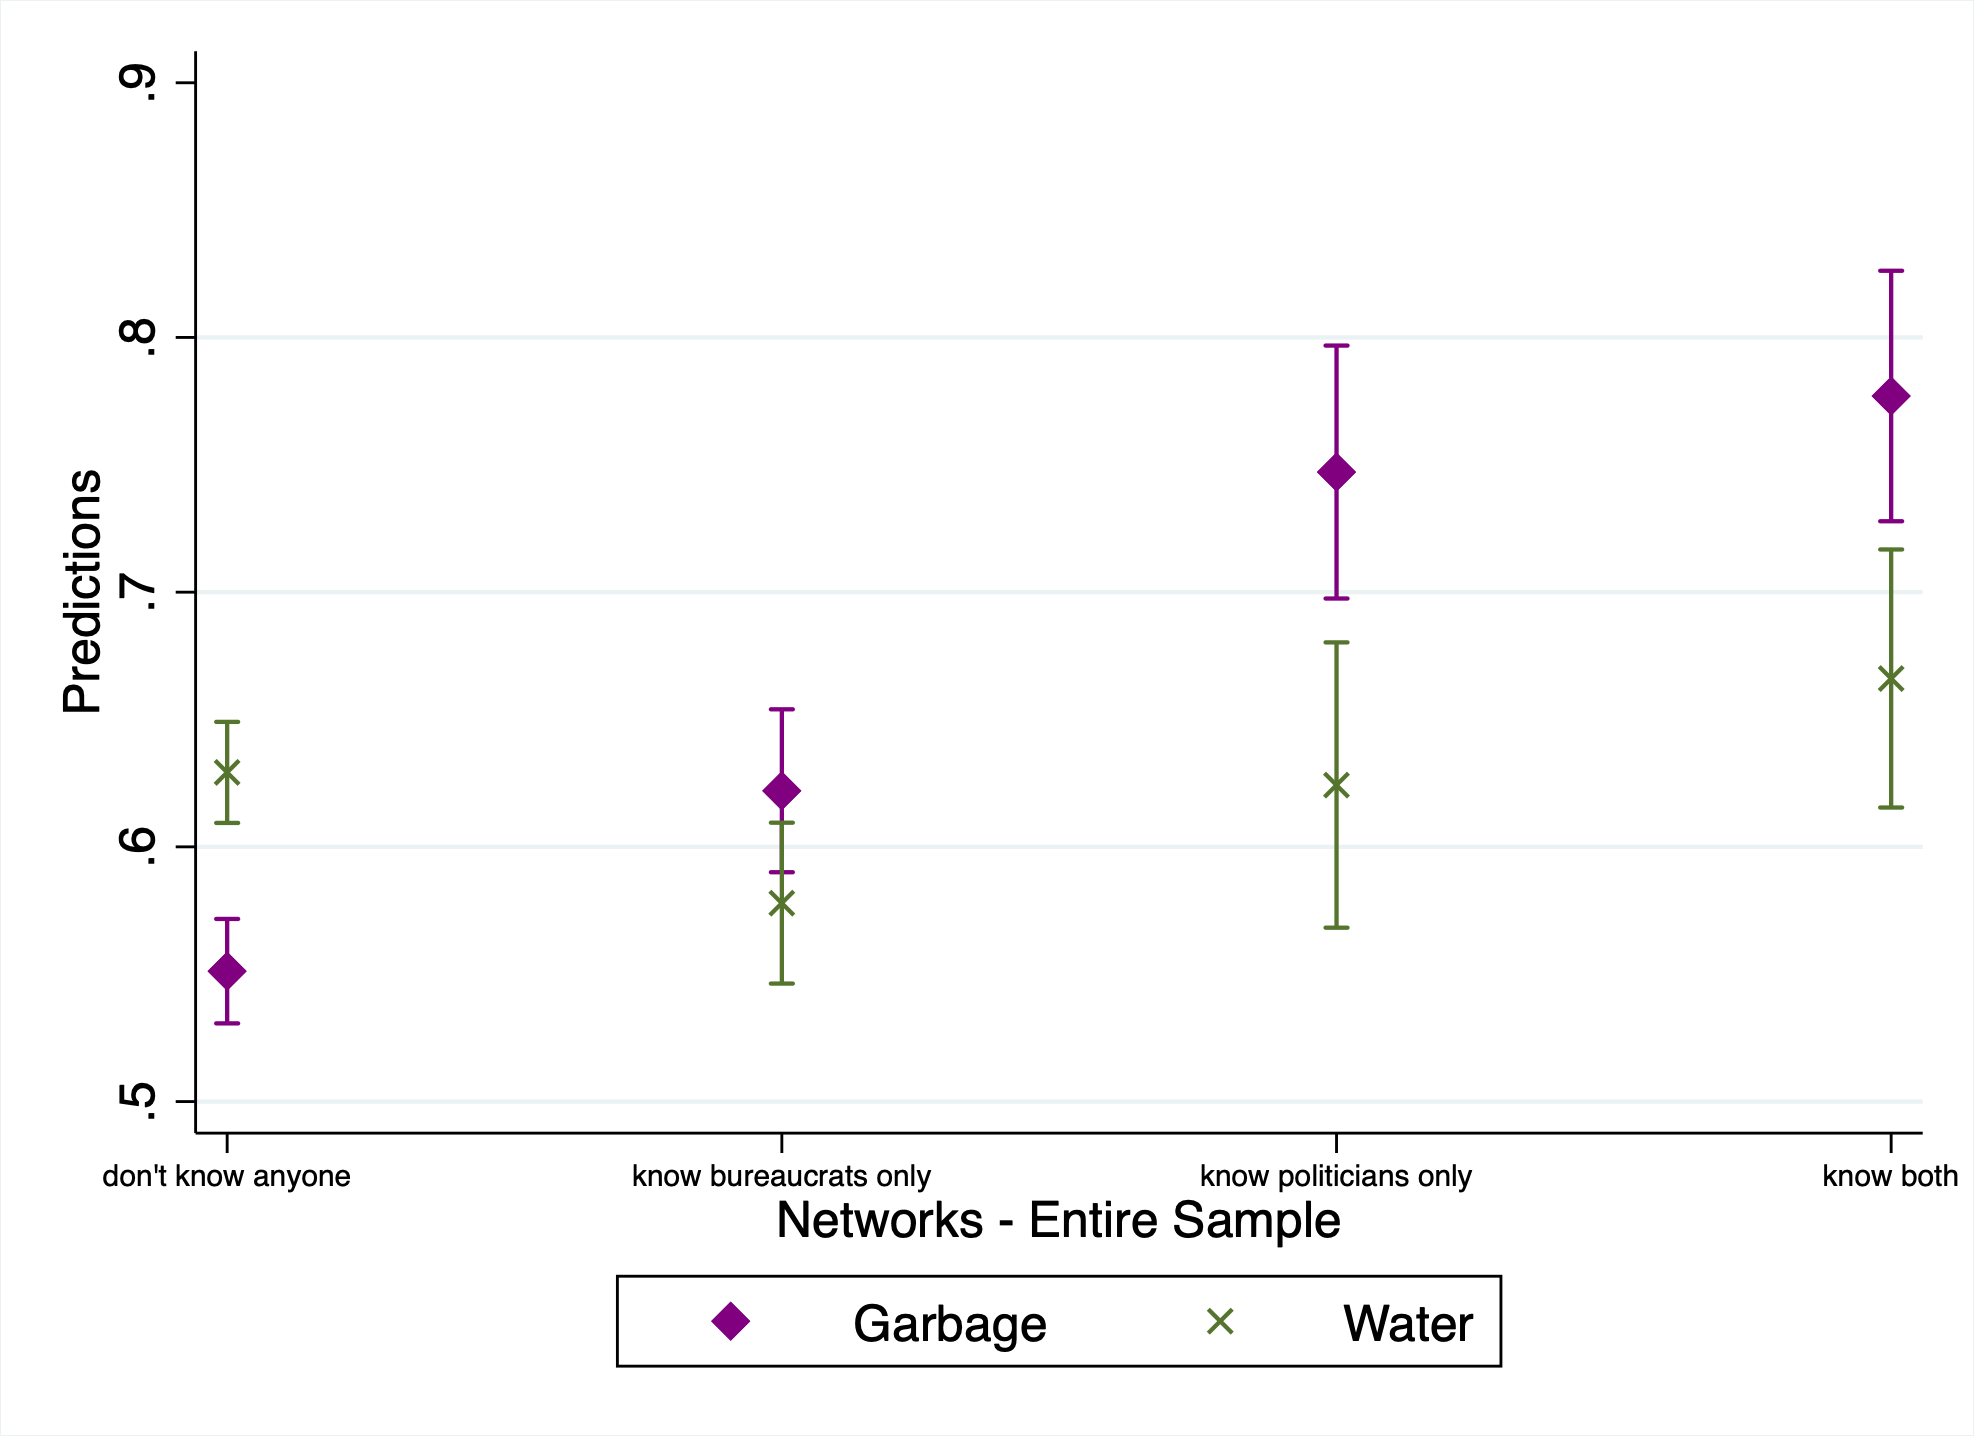
\includegraphics[scale=.4]{figures/Networks_entire sample.png}
    \caption{This figure illustrates the predicted marginal effects of network connections on access to both trash (purple diamonds) and water services (green Xs) across Bhopal and Lucknow combined. The Y-axis represents the predicted margins (the likelihood of receiving services), while the X-axis categorizes respondents based on their network connections (whether they know bureaucrats, politicians, or both). The error bars represent 95\% confidence intervals.}
    \label{fig:margins for non voting1}
\end{figure}



\begin{figure}[H]
    \centering
        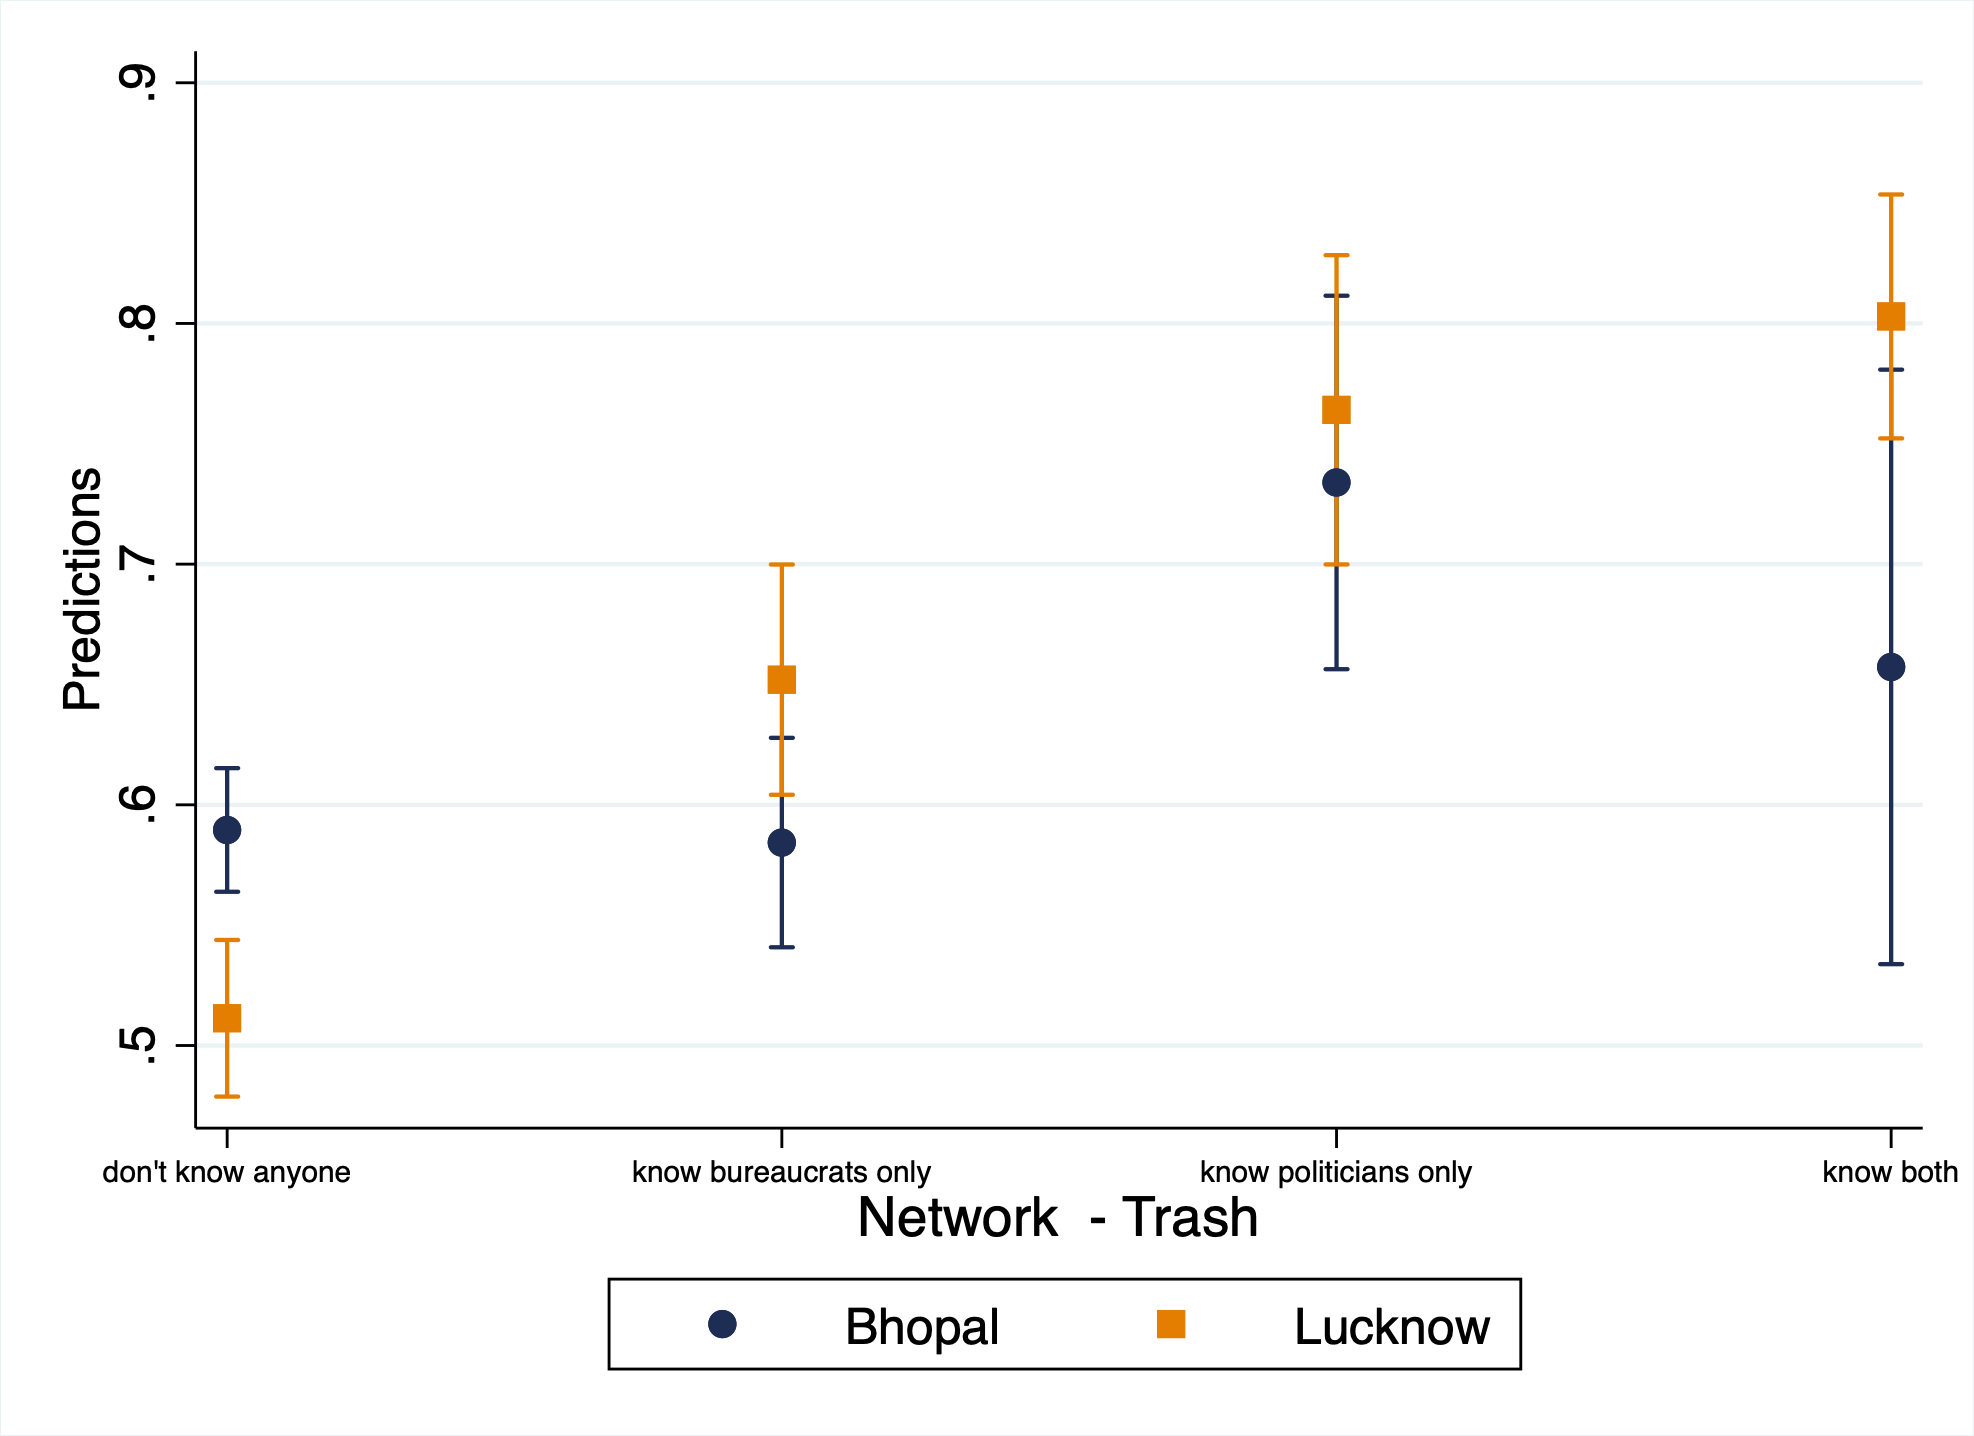
\includegraphics[scale=.4]{figures/Networks_trash.png}
    \caption{This figure illustrates the predicted marginal effects of network connections on access to trash for residents in Bhopal (blue circles) and Lucknow (orange squares). The Y-axis represents the predicted margins (likelihood of receiving trash services), while the X-axis categorizes respondents based on their network connections. The error bars represent 95\% confidence intervals.}
    \label{fig:margins for non voting}
\end{figure}

\begin{figure}[H]
    \centering
        \includegraphics[scale=.4]{figures/Networks_water.png}
   \caption{This figure illustrates the predicted marginal effects of network connections on access to water services for residents in Bhopal (blue circles) and Lucknow (orange squares). The Y-axis represents the predicted margins (likelihood of receiving water services), while the X-axis categorizes respondents based on their network connections. The error bars represent 95\% confidence intervals.}
    \label{fig:margins for non voting}
\end{figure}

\begin{figure}[H]
    \centering
    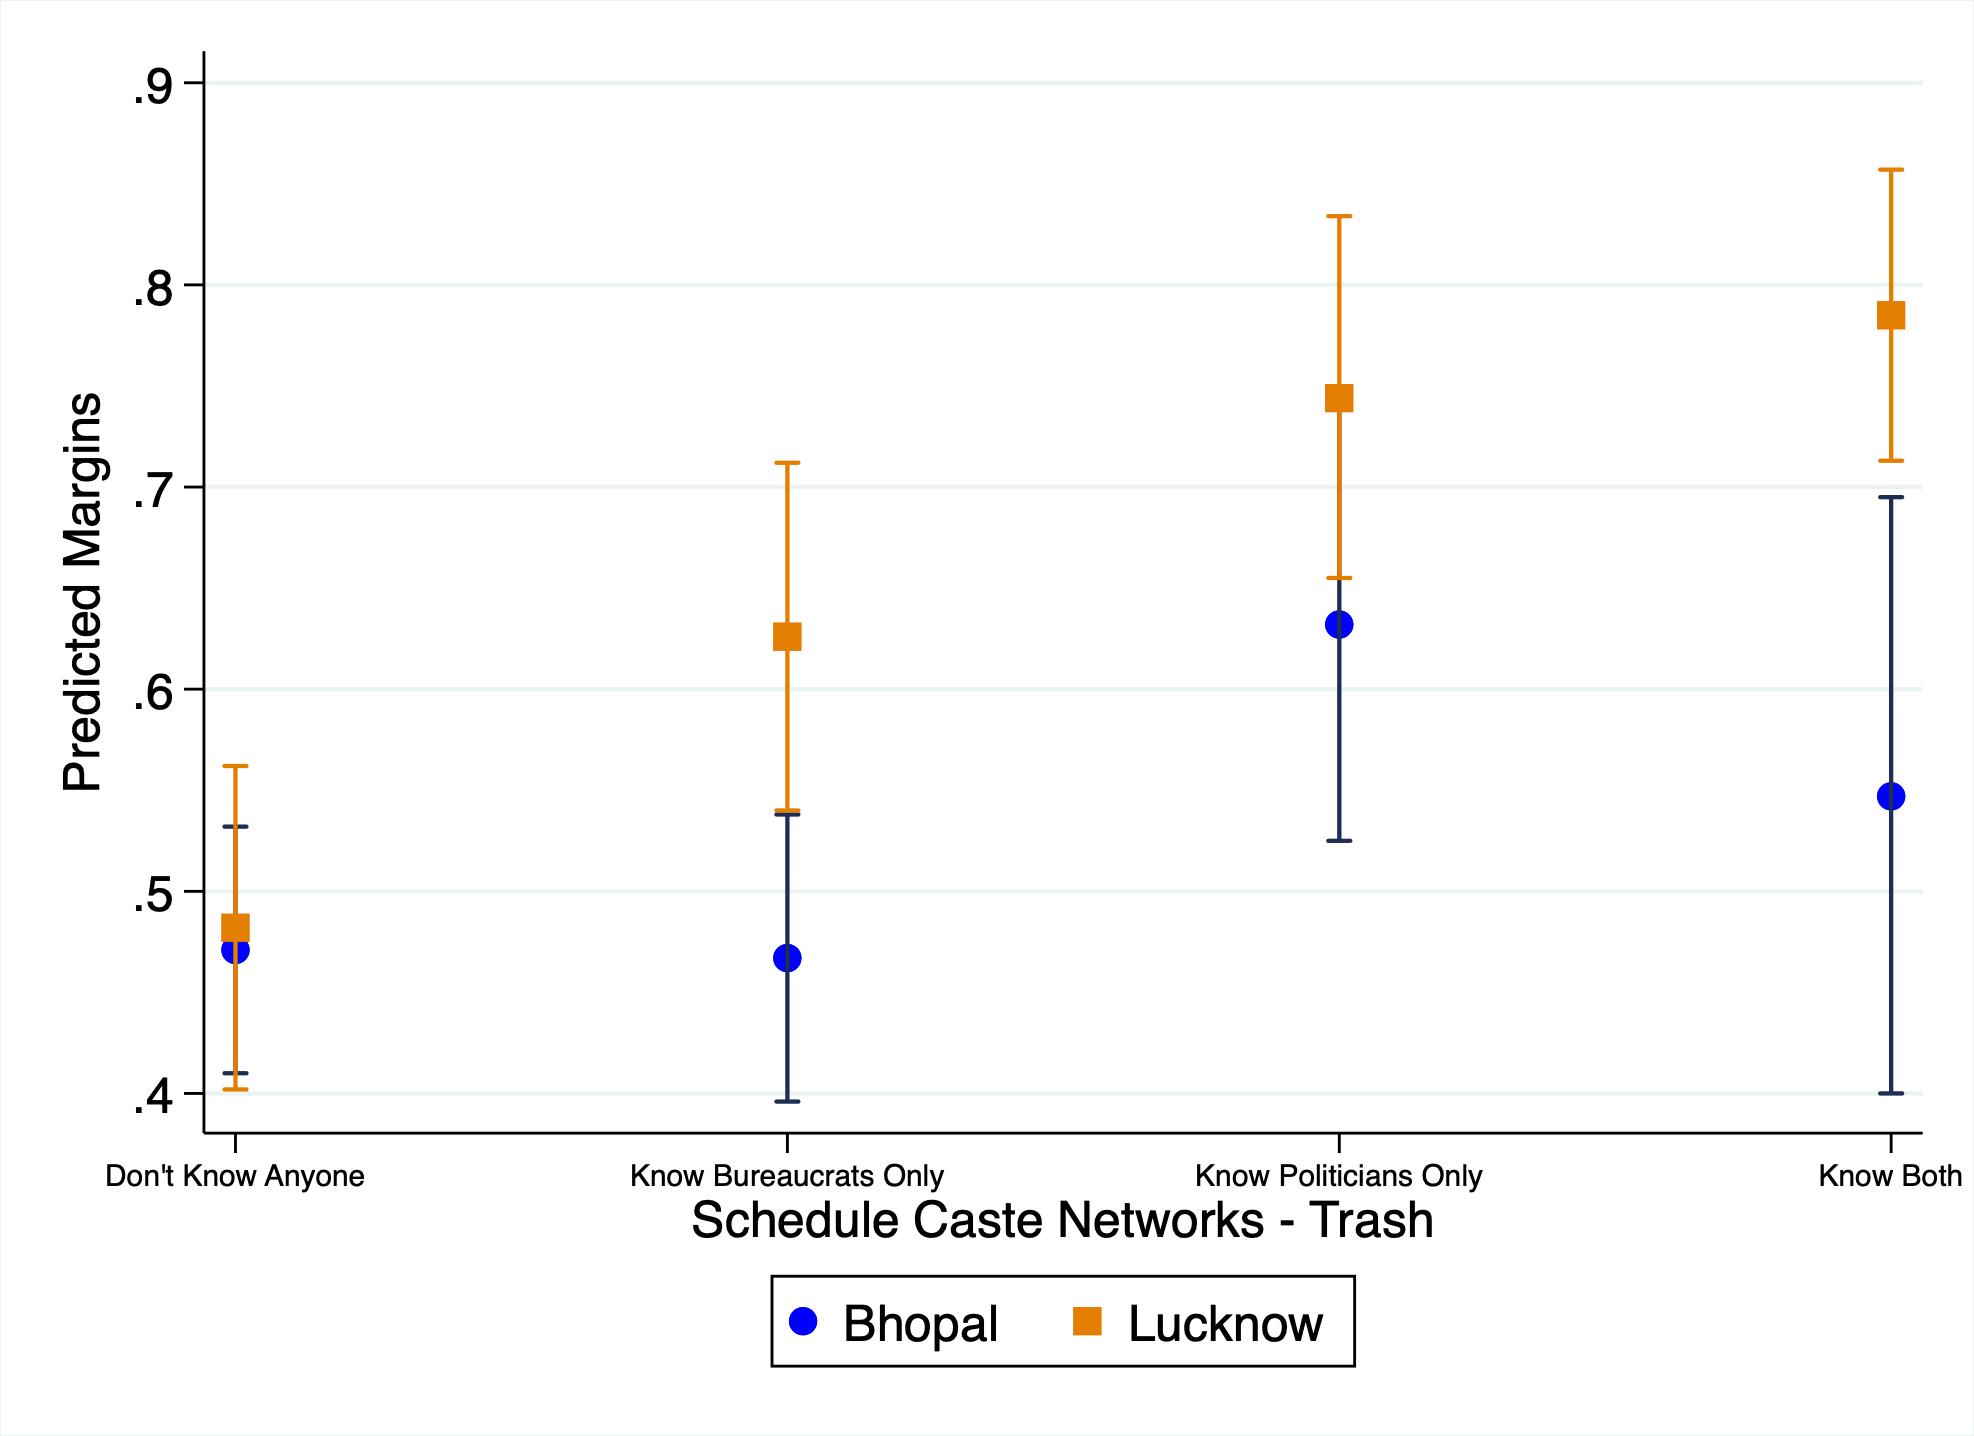
\includegraphics[scale=.4]{figures/Networks_trash_SC.png}
    \caption{SC Network - Trash: This figure displays the predicted marginal effects of different network connections (knowing bureaucrats, politicians, or both) on the likelihood of receiving trash services for Scheduled Caste (SC) residents in Bhopal (blue circles) and Lucknow (orange squares). The Y-axis represents the predicted margins (probability of receiving trash services), while the X-axis categorizes the different types of network connections. The error bars represent 95\% confidence intervals.}
    \label{fig:margins for non voting}
\end{figure}


\begin{figure}[H]
    \centering
        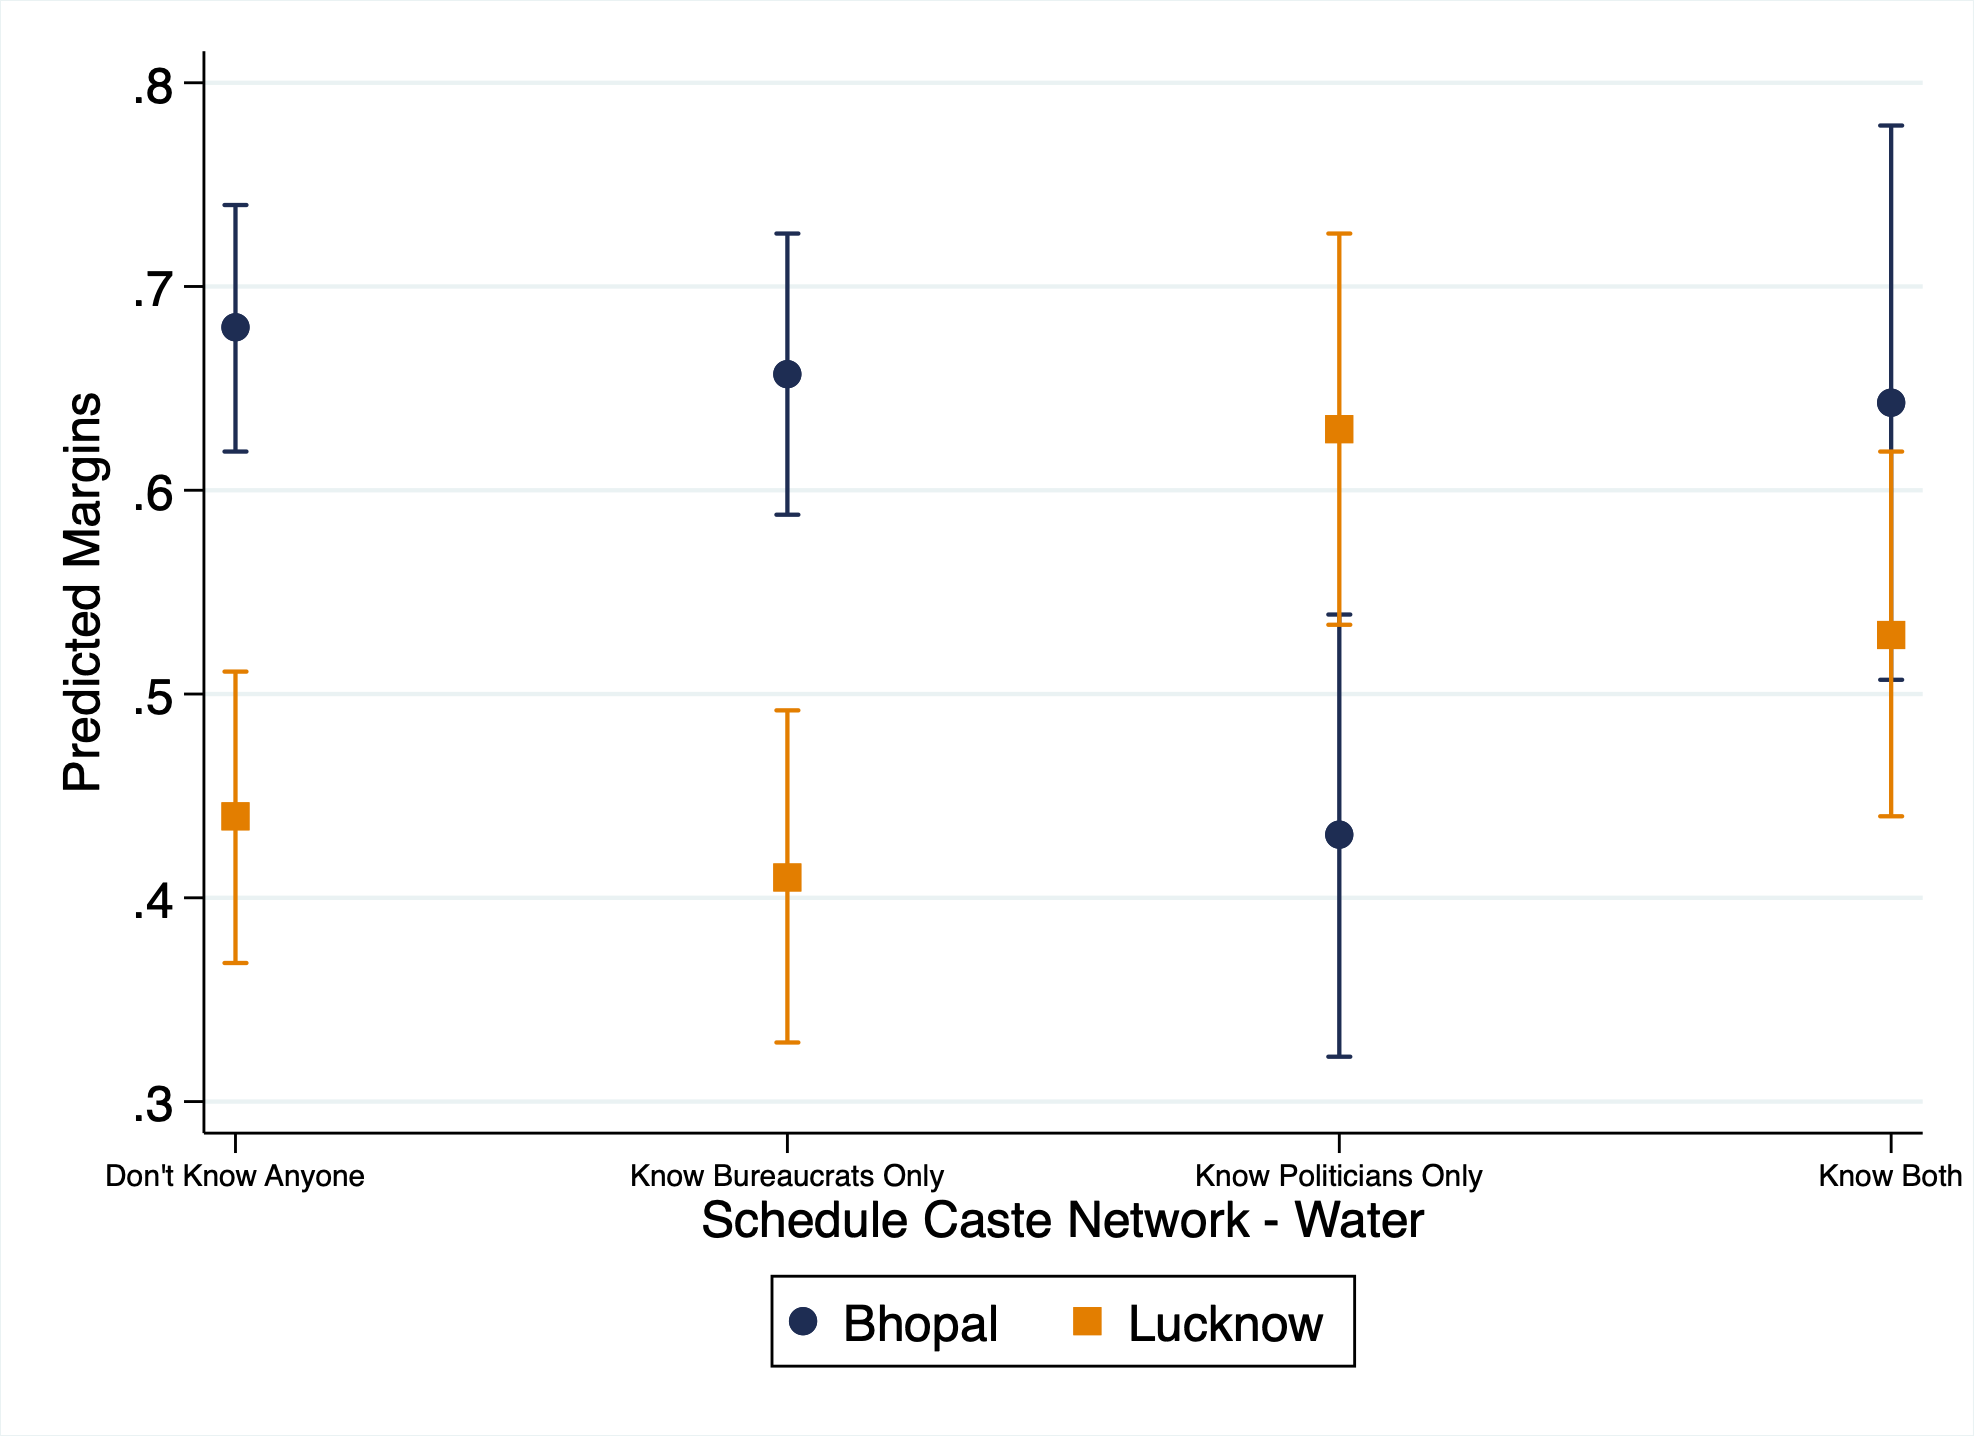
\includegraphics[scale=.4]{figures/Networks_twater_SC.png}
    \caption{ SC Networks - Water: This figure illustrates the predicted marginal effects of network connections on water service access for Scheduled Caste (SC) residents in Bhopal (blue circles) and Lucknow (orange squares). The Y-axis represents the predicted margins (probability of receiving water services), while the X-axis categorizes the different types of network connections. The error bars represent 95\% confidence intervals.}
    \label{fig:margins for non voting}
\end{figure}



\begin{figure}[H]
    \centering
    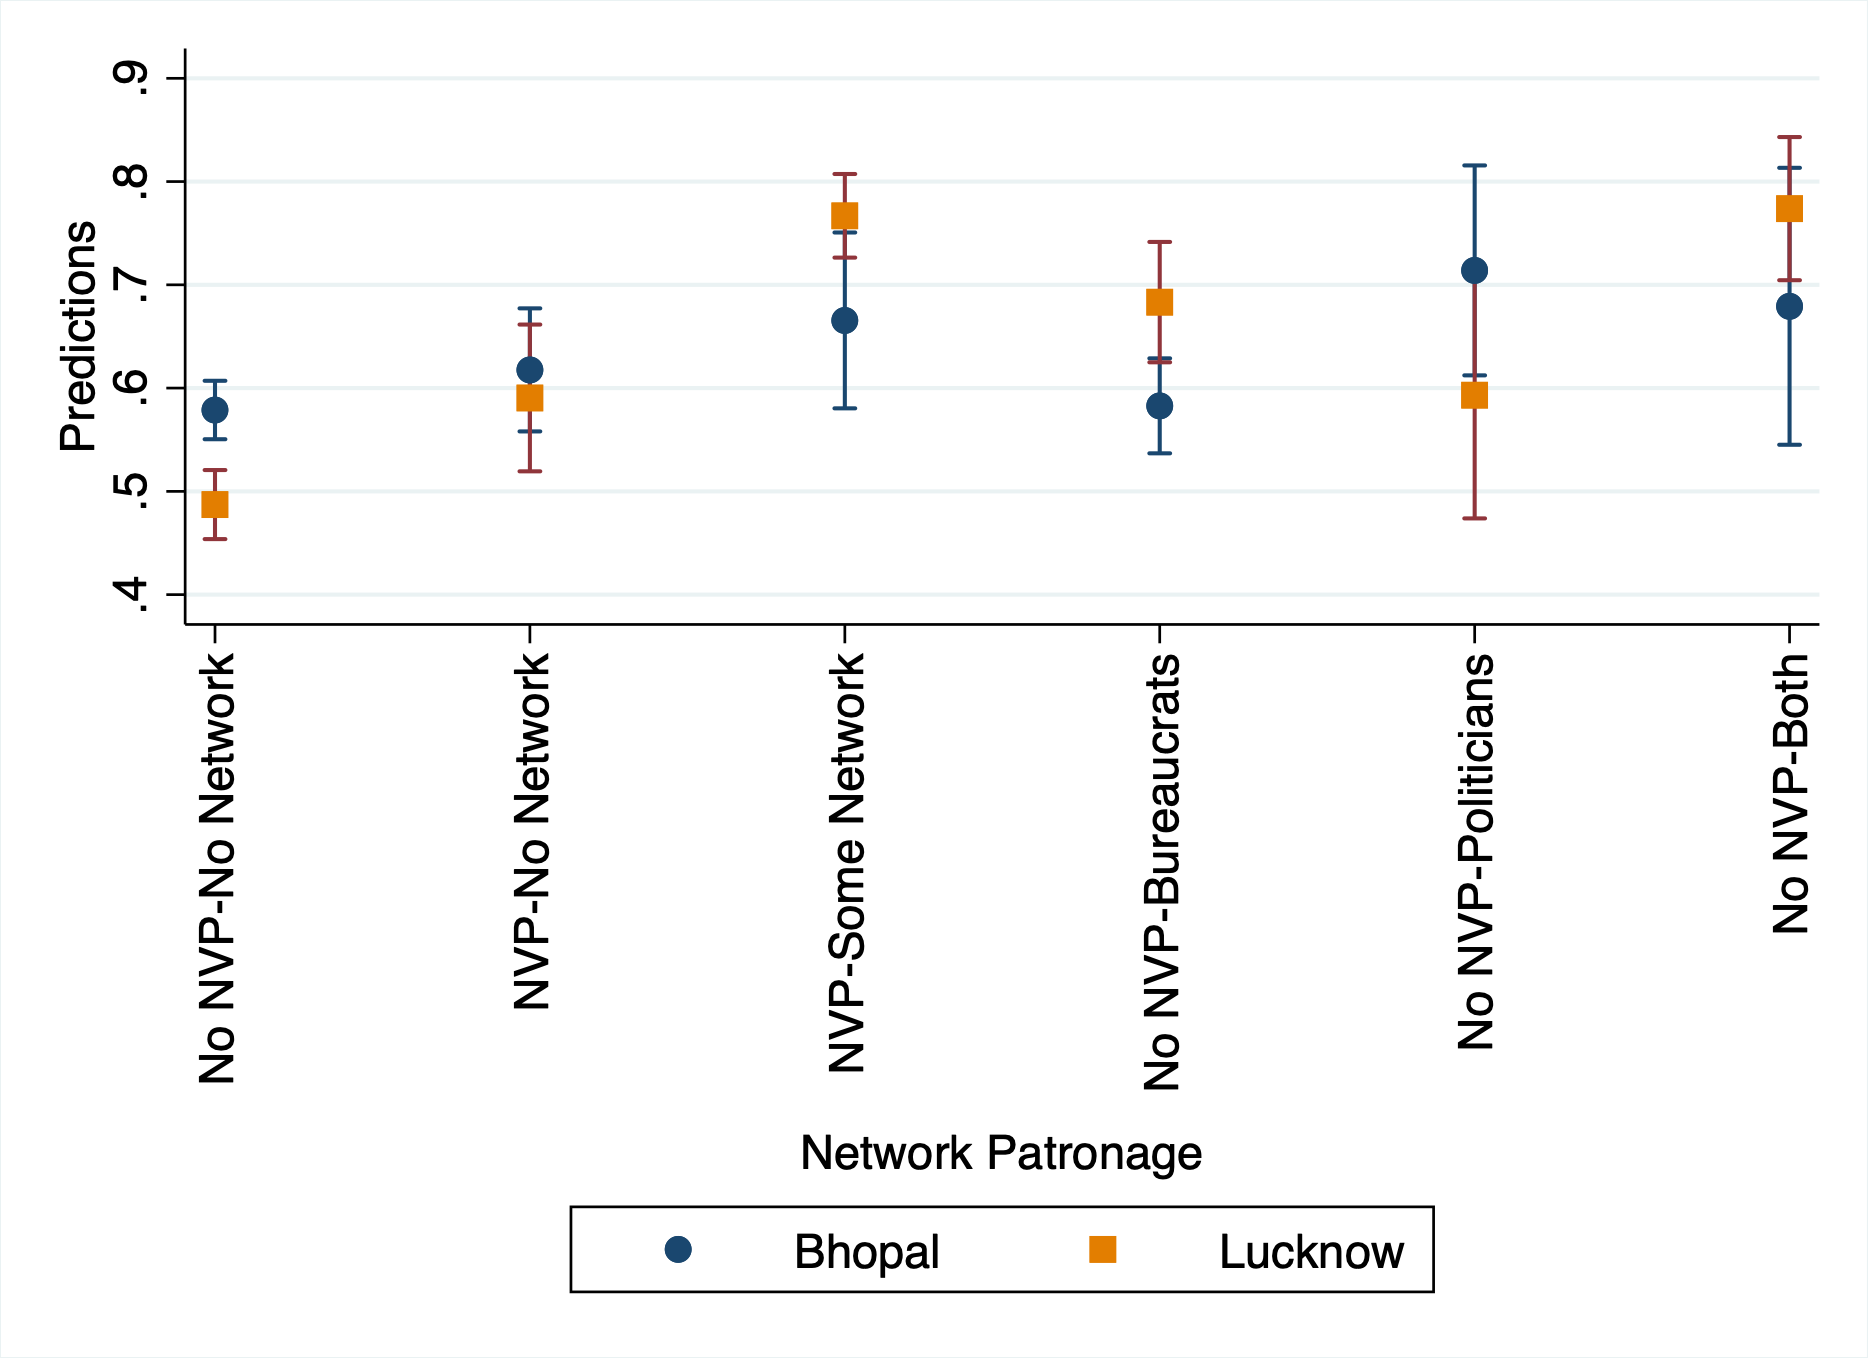
\includegraphics[scale=.4]{figures/NetPaT_garbage_.png}
    \caption{Predicted Margins of Networks and Political Participation on Trash Services: This figure shows the predicted marginal effects of different network connections (knowing bureaucrats, politicians, or both) and non-voting political participation (NVP) on trash services in Bhopal (blue circles) and Lucknow (orange squares). The Y-axis represents the probability of receiving trash services, and the X-axis categorizes: \textbf{No NVP-No Network: No participation or connections.} NVP-No Network: Political participation without connections.\textbf{NVP-Some Network: Political participation and connections.} No NVP-Both: No participation but with both bureaucratic and political connections.The error bars represent 95\% confidence intervals.}
    \label{fig:margins for non voting}
\end{figure}


\begin{figure}[H]
    \centering
        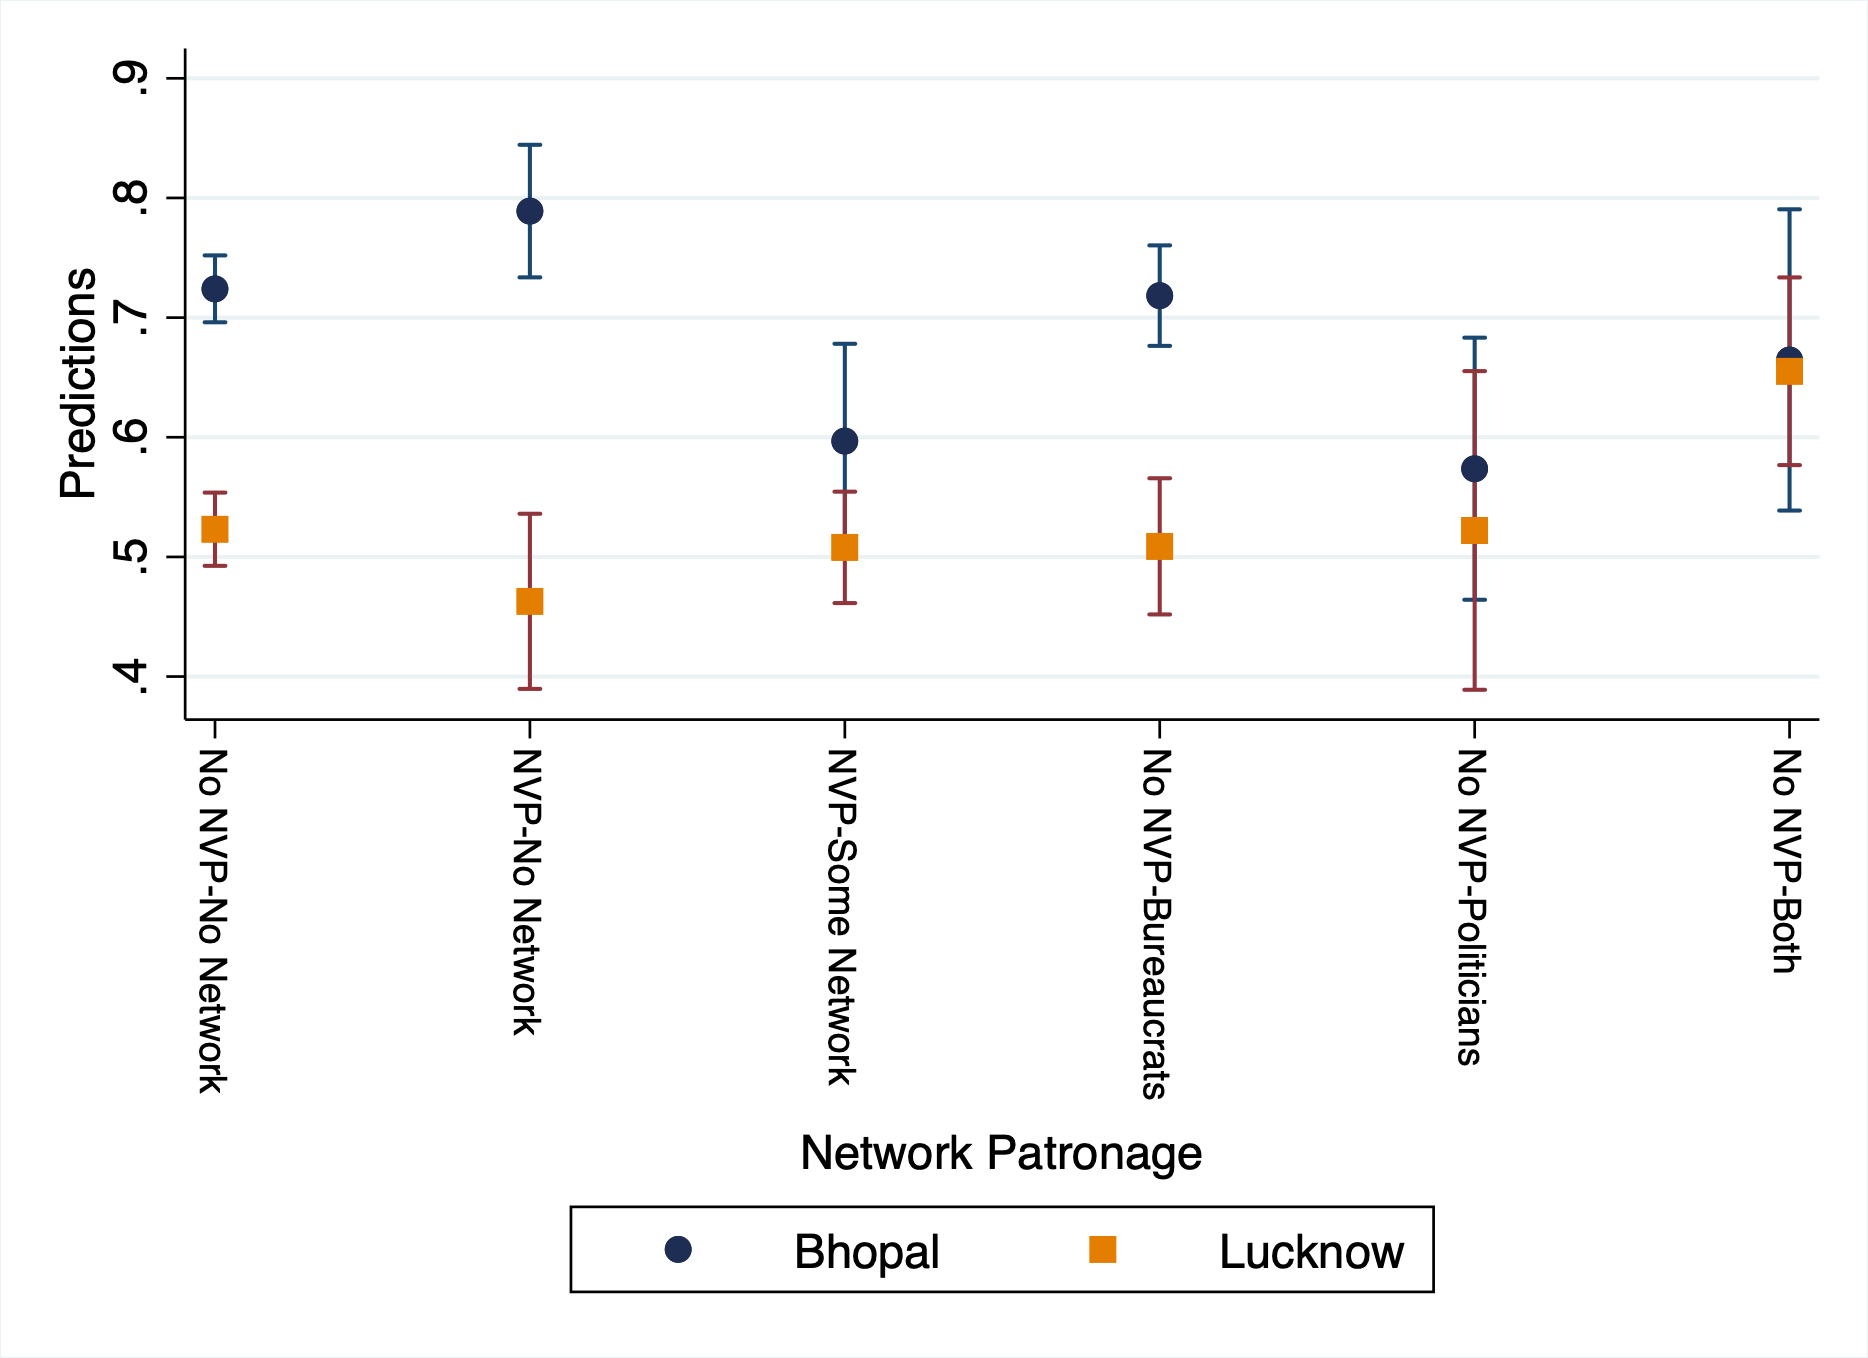
\includegraphics[scale=.4]{figures/NetPaT_water_.png}
    \caption{ Predicted Margins of Networks and Political Participation on Water Services: This figure shows the predicted marginal effects of different network connections (knowing bureaucrats, politicians, or both) and non-voting political participation (NVP) on water services in Bhopal (blue circles) and Lucknow (orange squares). The Y-axis represents the probability of receiving water services, and the X-axis categorizes: \textbf{No NVP-No Network: No participation or connections.} NVP-No Network: Political participation without connections.\textbf{NVP-Some Network: Political participation and connections.} No NVP-Both: No participation but with both bureaucratic and political connections.The error bars represent 95\% confidence intervals.}
    \label{fig:margins for non voting_2}
\end{figure}

\subsection{Taking stock}



The comparative analysis of public service delivery in Bhopal and Lucknow illuminates critical variations in institutional performance despite similar formal governance structures. The baseline disparities are substantial: Lucknow residents face 19.7\% lower odds of receiving trash services and 56.4\% lower odds of receiving adequate water services compared to Bhopal, suggesting fundamental differences in service delivery mechanisms between the cities.

In contexts of constrained institutional capacity, social networks with political and bureaucratic actors emerge as crucial determinants of service access. However, the efficacy of these networks varies systematically with service characteristics. Trash collection, being discretionary and municipally controlled, demonstrates high responsiveness to both political participation and bureaucratic-political networks. This is particularly evident in Lucknow, where densely engaged citizens (those combining political participation with official networks) see their probability of access increase from 49\% to 77\%. Notably, marginalized groups like Scheduled Caste residents can leverage these networks to increase their access probability from 50\% to 82\%, suggesting that patronage systems, paradoxically, may facilitate service access for historically excluded groups in contexts of weak institutional capacity.


Water services, however, demonstrate the limitations of network-based access to complex public goods. Even citizens with strong political engagement and extensive networks struggle to significantly improve their water access in Lucknow, where the baseline probability remains at 50\% with only marginal improvements through networks. This contrasts markedly with Bhopal's consistently high water access (73\%) independent of network effects. The infrastructure-intensive nature of water provision, requiring inter-governmental coordination and technical expertise, appears relatively impervious to individual-level interventions.


To circle back, while our theoretical framework suggests that politicians (driven by electoral accountability) and bureaucrats (focused on technical expertise and long-term stability) must collaborate for effective service delivery, the empirical evidence reveals starkly different outcomes across cities and services. Why do similar institutional contexts produce different coordination patterns? How can patronage networks successfully deliver trash services without excluding marginalized groups, yet fail to facilitate the coordination necessary for complex services like water? 

The following qualitative analysis explores these questions by examining the historical evolution of trash and water systems in both cities, seeking to understand why one system developed along patronage lines while the other became programmatic, and why patronage networks, despite their success with simpler services, fail to enable the coordination necessary for universal access to complex services.

\section{Politician-Bureaucrat Coordination - Patronage or Programmatic: Understanding the Mechanism}

\vspace{5mm}

\subsection{Water Services}
This section examines how divergent institutional arrangements in Bhopal and Lucknow led to different outcomes in water service provision, despite similar starting conditions. While both cities showed comparable levels of tap water access in 1981, 1991, and 2001, their trajectories began diverging notably after 2011, with recent citizenship surveys indicating an expanding gap in service coverage.

\begin{figure}[H]
    \centering
        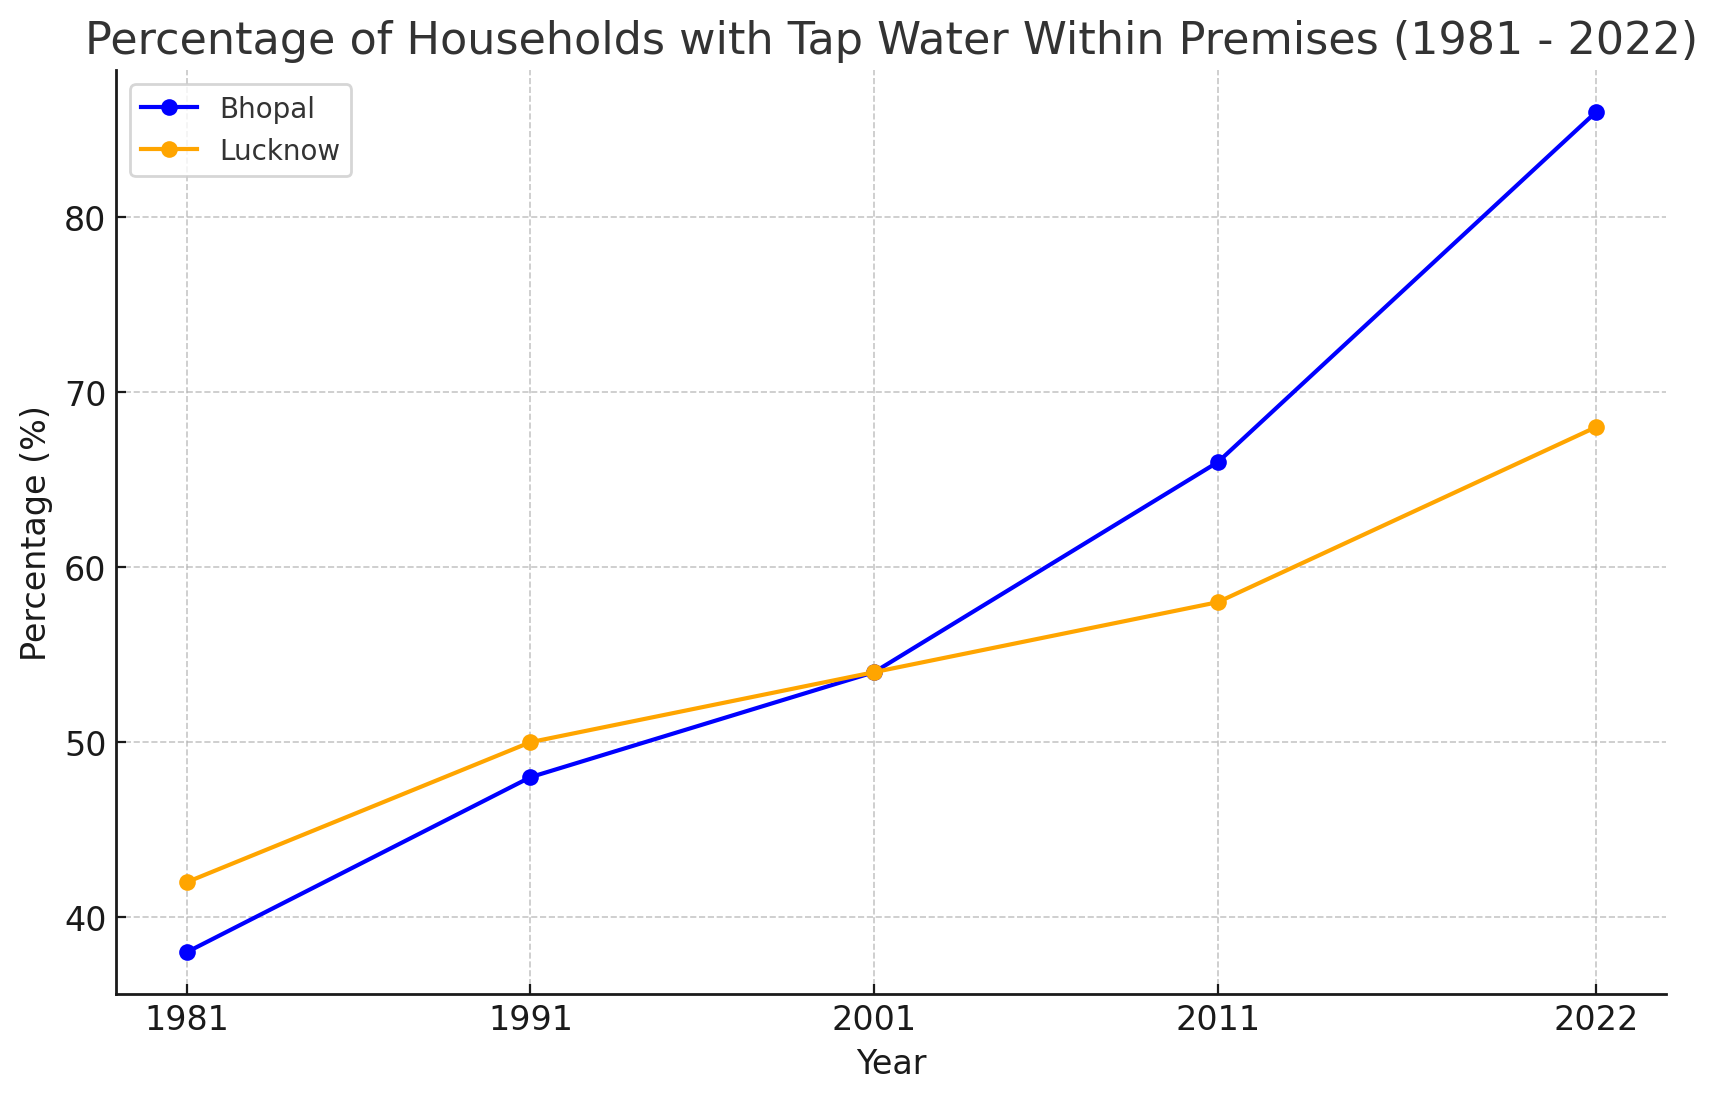
\includegraphics[scale=.65]{figures/output.png}
    \caption{Change in Tap water across Bhopal and Lucknow. Data for 1981-2011 is from the Census of India, 2022 is from Household Survey}
    \label{fig:margins for non voting_2}
\end{figure}

The introduction of India's first national urban renewal program in 2004, the Jawaharlal Nehru Urban Renewal Mission (JnNURM), provided a critical juncture for both cities. However, their institutional responses to this opportunity differed substantially, shaped by local political economies and bureaucratic arrangement

\vspace{5mm}
\textbf{Lucknow}

Lucknow's struggle with water service delivery illustrates how institutional fragmentation and competing political interests can undermine urban service provision. Despite the launch of India's first national urban renewal program (Jawaharlal Nehru Urban Renewal Mission or JnNURM) in 2004, which provided cities with both financing and incentives for universal water access, Lucknow's institutional landscape proved resistant to meaningful reform. This institutional dysfunction manifested across multiple dimensions, from political resistance to price reforms to organizational fragmentation in service delivery.

At the political level, there was a notable disconnect between local and elite politicians regarding water pricing reforms. While local politicians demonstrated some openness to revenue enhancement, acknowledging its potential to improve services through measures like the 2014 City Council's approval of "an 8\% increase in prices of water per the report of the commissioner," \footnote{Lucknow City Government meeting archives. Accessed from the Lucknow Nagar Nigam in 2021} elite politicians actively resisted such changes. This resistance was exemplified by Urban Development Minister Mohd. Azam Khan's categorical rejection of water meter installations across major UP cities \footnote{Azam Khan Opposes Water Meter Installation," \href{https://timesofindia.indiatimes.com/city/lucknow/azam-khan-opposes-water-meter-installation/articleshow/22306030.cms}{The Times of India, September 5, 2013}}. In a personal interview, the then Minister justified this position by arguing that "the funds required for such installations would have been more effectively used to improve drinking water supply in underdeveloped urban neighborhoods.\footnote{Interview with Md. Azam Khan, Minister for Urban Development 2012-2017, Rampur Jail 2022}" This stance reflected a broader political reluctance to implement pricing reforms, even when they were tied to development funding.

The institutional challenges were particularly evident in the operations of the Lucknow Jal Sansthan (LJS), established in 1975 to manage the city's water resources \footnote{The Uttar Pradesh Water Supply and Sewerage Act, 1975 (Act 43 of 1975), enacted by the Uttar Pradesh Legislature, provides the legal framework for the establishment and regulation of water supply and sewerage services in the state, including the creation of the Uttar Pradesh Jal Nigam and local Jal Sansthans to manage these services.
}. Despite its intended design as an autonomous entity, the LJS has struggled with limited financial independence, remaining heavily dependent on state grants even for basic operational expenses. This financial constraint was exacerbated by the Uttar Pradesh government's rural-centric budget allocation, which left urban water bodies with minimal resources\footnote{With 78\% of Uttar Pradesh being rural, the state's water management priorities and budget allocations heavily favored rural areas. This bias is starkly evident in the budget allocation: of the total INR 17,000 crore (\$2.014 billion) , the rural sector received 15,000 crore (\$1.778 billion), while the urban sector was allocated a mere 2,000 crore (\$0.237 billion). Uttar Pradesh Budget Analysis 2021-22," \href{https://prsindia.org/budgets/states/uttar-pradesh-budget-analysis-2021-22}{PRS Legislative Research}, accessed November 18, 2024}. Attempts to reform this structure through initiatives like merging and then re-separating urban and rural water bodies failed to address these fundamental issues, leaving the LJS in a perpetual state of financial and operational vulnerability \footnote{About Rural Jal Nigam," Uttar Pradesh Jal Nigam, accessed November 18, 2024,}. The dysfunction extended to project implementation and inter-organizational relationships. Efforts to integrate the LJS into the Lucknow Municipal Corporation (LMC) structure encountered significant resistance, with LJS employees expressing concerns about maintaining operational autonomy and service quality \footnote{Employees of Lucknow Water Department Formed a Front Against Being Absorbed in Lucknow Municipal Corporation," \href{ https://www.amritvichar.com/article/405452/employees-of-lucknow-water-department-formed-a-front-and-wrote#gsc.tab=0}{Amrit Vichar}, accessed November 18, 2024,}. The unusual reporting structure, where the LJS General Manager remained under UP Jal Nigam authority rather than city officials, created additional layers of complexity and hampered coordinated action \footnote{ Interview with Arvind Kumar Giri, Under Secretary, Uttar Pradesh. Lucknow 2022}.

What further complicated matters was the complete marginalization of LJS, the primary water service provider, in the implementation of major water projects under the union government's funding program. Instead of leveraging the institutional knowledge and expertise of LJS, the state government decided to locate the project management unit within the state's Urban Development Department \footnote{Evaluation Report: India Financial Institutions Reform and Expansion–Debt and Infrastructure Ex-Post Evaluation, WASH Ex-Post Evaluation Series—Water Communications and Knowledge Management (CKM) Project, September 2018, 11, 13}. This decision not only reflected a deep distrust of city-level institutions but effectively sidelined the very organization meant to provide water services \footnote{Interview with PK Srivastava, Additional Municipal Commissioner LMC 2009-2013, Lucknow 2022
}. Elite bureaucrats at the state secretariat, wary of potential political-contractor nexus at the city level, deliberately kept both city politicians and bureaucrats at arm's length from the project implementation\footnote{ibid.}\footnote{Interview with MG Ramachandaran, Urban Development Secretary 2004-2009, Government of India. Delhi 2023}. However, this attempt to centralize control paradoxically led to a situation where those most familiar with the city's water infrastructure and needs - the LJS officials - were excluded from critical decision-making processes\footnote{Final City Water Plan for Lucknow, 2011}.\footnote{Interview with SK Singh, PCS officer, Head of Lucknow Jal Sanshthan 2007-2012. Delhi 2023
}

The resulting vacuum in local expertise became evident in project implementation. With the LJS marginalized and city government stripped of meaningful policy-making power, state-level bureaucrats found themselves having to arbitrate between competing interests without adequate ground-level understanding. The critical decision of where to initially implement the water project - whether to attempt city-wide coverage or focus on the older areas that formed the core of the city government's political base - became a contentious issue precisely because those making the decisions lacked the local context that LJS could have provided.
The site selection process for water projects became particularly contentious, exposing these institutional fault lines. While DFID and the Urban Development Department prioritized newly incorporated areas like Gomti Nagar and Transport Nagar, the Lucknow Municipal Corporation advocated for older, central neighborhoods, reflecting local political interests\footnote{International Financial Institutions as part of the reform to fund projects. In Bhopal, ADB and the UK's Department for International Development (DFID) were active in urban projects. Meanwhile, in Uttar Pradesh, USAID's FIRE-D project worked on urban reforms. These IFIs promoted city development plans, market-based infrastructure financing, and capacity building reforms. In the case of Lucknow, FIRE-D USAID were responsible, and while  the major funding went to water related projects}. This disagreement was further complicated by disputes over contractor selection, where political affiliations played a significant role. The state's ruling Samajwadi Party favored Emaar Construction Limited, a Dubai-based firm, while the BJP-controlled LMC preferred a local bidder \footnote{Interview with Kaushal Shankar Pandey (INC) , councilor from Aliganj ward. Lucknow 2022
} \footnote{Interview with Md. Saifullah, Councillor for the Yadunath Sanyal ward from 2006-2017, Lucknow 2022}. These conflicts ultimately led to DFID's withdrawal from the project, as they feared both contract violations and the potential precedent this might set for future collaborations \footnote{Interview with RK Srinivasan, USAID Water, Sanitation and Hygiene Finance (WASH-FIN) Delhi 2023
}. While the Asian Development Bank chose to continue their involvement, they significantly reduced their financial commitment by half. \footnote{Office of the Principal Accountant General (General & Social Sector Audit), Uttar Pradesh. (2016). Annual Technical Inspection Report on Urban Local Bodies for the Year Ended 31 March 2016 (p. 23, 24)}

The city's experience with water project implementation underscores a critical insight about urban governance: even when funding is available, institutional fragmentation can severely impair project execution. DFID officials repeatedly advised elite bureaucrats in the state Secretariat that municipal management would enhance project effectiveness, but these recommendations were largely ignored. After two years of limited progress and unresolved disagreements over key issues, DFID's decision to exit the project entirely reflected the severity of these institutional challenges\footnote{Interview with RK Srinivasan, USAID Water, Sanitation and Hygiene Finance (WASH-FIN) Delhi 2023}.

\vspace{5mm}
\textbf{Bhopal}

Bhopal faced similar pressures regarding water charges, with both elite and city politicians initially resistant to reforms. However, the city's approach to implementing the union government's water program differed significantly from Lucknow's, largely due to its constrained financial position \footnote{Interview with Deepti Gaur Mukherjee, Indian Administrative Services, Commissioner Bhopal Municipal Corporation, 2009-2011. Bhopal 2022}. While both cities were starved for money, Lucknow, as a constituency of a former prime minister, believed it could secure funding through alternative political channels\footnote{Interview with SK Shastri, Officer on Special Duty to A.B. Vajpayee, Prime Minister of India (2009-2014) and three time member of Parliament from Lucknow. Delhi 2023}. Bhopal held no such primacy, forcing a more pragmatic approach. As one consultant noted, "Cities in Madhya Pradesh were not pushovers. The Mayors knew they were powerful and maintained independence from the state leadership."\footnote{Interview with Arkaja Singh, a private consultant with experience working with various International Financial Institutions and was a consultant hired by DFID for UDAY. Delhi 2022
} Unlike Lucknow, where decision-making shifted to the secretariat, Bhopal's institutional actors recognized that the union government's plan represented their only viable path forward for improving water services, creating pressure for internal alignment between state and city institutions \footnote{Interview with Deepti Gaur Mukherjee, Indian Administrative Services, Commissioner Bhopal Municipal Corporation, 2009-2011. Bhopal 2022}.

A crucial difference emerged in how the Project Management Unit (PMU) for the water projects in the 2000s was positioned and operated. While both cities received support from ADB and DFID for establishing PMUs, Bhopal's unit was situated within the city government (Bhopal Municipal Corporation or BMC) rather than at the state level\footnote{Interview with Priyanka Das, Indian Administrative Services, Madhya Pradesh Cadre. Bhopal 2022}. This positioning proved critical as it enabled direct collaboration with the state level bureaucracy - officers from the Madhya Pradesh Municipal Administration Services, a cadre dedicated exclusively to urban administration\footnote{nterview with Neelesh Dubey, Madhya Pradesh Municipal Administrative Services. Bhopal 2022
}. These career bureaucrats, operating under the City Commissioner's authority, brought crucial urban expertise to project implementation \footnote{Madhya Pradesh Urban Services for the Poor (MPUSP) Project. (2012). Project completion review: Madhya Pradesh Urban Services for the Poor (MPUSP) Project. Retrieved from https://iati.fcdo.gov.uk/iati_documents/3780260.odt.}.

The effectiveness of this arrangement was highlighted by Bruce Pollock,  head of the DFID project for Madhya Pradesh. He particularly emphasized the role of these officers, noting that "they were really the core of the program in Bhopal, whose negotiating skills - got the work done." Explaining further the unique value these state-appointed bureaucrats brought: "These guys had been trained in the PMU to understand the legalistic aspects of contracts but they added their knowledge of the local landscape. They identified builders, who had political connections or politicians open to contract negotiations. This could not have been done either by us (meaning the international agency) or the Commissioners (elite IAS officers)." \footnote{Interview with Bruce Pollock, who headed the DFID program in Madhya Pradesh from 2008 to 2013. As one observer noted, "These officers moved from one city to another but were retained in the PIU, so we knew we could rely on training a select group of officers which, even if transferred, would remain part of the system.” Zoom 2021, 2022,2024.
}

The implementation of the \$28 million ADB/DFID-funded water project in 2007 illustrates how Bhopal's institutional arrangement facilitated effective navigation of competing interests. The project faced multiple stakeholder demands: politicians sought coverage for their areas and contracts for associates, ADB/DFID pushed for equitable network distribution, and bureaucrats, particularly engineers, had their own interests in contracts and licenses\footnote{ibid.}. Rather than allowing these competing interests to paralyze implementation, Bhopal's state level bureaucracy became a key player in making the program operational\footnote{Project Uday. (n.d.). Project management. Retrieved from https://web.archive.org/web/20180828214026/http://projectuday.gov.in/ProjectMgt.htm}.

The then Mayor of Bhopal, Sunil Sood, explained that local contractors were a vital part of the process and an essential component of the political ecosystem. While elite IAS officers were aware of these dynamics, they were reluctant to engage directly.\footnote{nterview with Sunil Sood, Congress led Mayor of Bhopal City Government (2004-2009), Leader of Bhopal City Council (2000-2004),, City Councillor (1995-2009) } As Manish Singh, the then IAS officer posted as Commissioner of BMC, explained, "You can understand the implications of getting these contractors in the office. Negotiating is not my job, but I did ask my deputies to look into this – they knew the landscape better. The guidelines were clear; either get it passed in the house or surrender the project, so s\textit{omeone had to do the dirty job}."\footnote{Interview with Manish Singh, Indian Administrative Services, Madhya Pradesh Cadre. Bhopal 2022
}

The resolution came through the joint efforts of state level bureaucracy and politicians. Abhay Ranjan Gowankar (then Assistant Commissioner, Administration in the BMC) and Devinder Chauhan (current Officer on Special Duty to Minister of Urban Development, Madhya Pradesh and then Deputy Project Coordinator of JnNURM) worked with Mayor Sunil Sood to find middle ground, making the project compatible with local realities. This involved assisting local contractors in meeting technical bid requirements and organizing meetings with stakeholders, including Louis Berger, one of the three international firms being considered for the water tender.\footnote{Throughout this research, I conducted interviews with a diverse range of stakeholders, and certain names repeatedly emerged as influential figures. This recurring mention was triangulated through official records, including meeting minutes from the Municipal Corporation, reports from third-party entities such as DFID, and input from government officials and political party representatives. Additionally, independent citizens actively engaged in local affairs provided further assessment and context. While these observations are based on interviews conducted with various stakeholders, the frequent mention of specific officers’ names underscores their significant role in local governance discussions during this period.}

Over multiple meetings, which stakeholders referred to as aligning "vision," state bureaucrats helped contractors and politicians devise implementation strategies.\footnote{Interview with Vivek Aggarwal, Louis Berger Limited. Delhi, 2023.
} They broke the project into smaller "packages" - manageable components like pipelines, road drains, culverts, or constructing local offices - making local contractors eligible for participation.\footnote{Iterview with Vijay Datta, JnNURM incharge, Urban Development and Housing Department, Madhya Pradesh Government, Bhopal, 2023.
}The bureaucrats also mediated with engineers to "reduce" bribes from contractors (referred to as cut money), recognizing the contractors' need to invest in better human and tech resources.\footnote{Interview with Devendra Chauhan, Madhya Pradesh Municipal Administrative Services, who was then with the BMC and is now an Officer on Special Duty (OSD) to the Minister of Urban Development. Bhopal 2023}\footnote{nterview with Arkaja Singh, a private consultant with experience working with various International Financial Institutions and was a consultant hired by DFID for UDAY. Delhi 2022
} Politicians, in turn, reassured councillors by ensuring their contractors were included in other projects like the water tender.

This pragmatic approach continued into recent times. In 2022, during the implementation of AMRUT 2 (JnNURM's successor) projects for dumpsite cleaning and housing construction, similar negotiations occurred between contractors and the Mayor in Council members. Being present in these discussions, some of them focused on organization, others explicitly addressed the distribution of illicit payments across bureaucratic and political networks.

\vspace{5mm}
\textbf{To summarise: }
The contrasting experiences of these cities illuminate two distinct patterns of politician-bureaucratic  coordination. In Lucknow, while city-level bureaucrats and politicians maintained their own coordination mechanisms, they failed to effectively navigate multiple levels of the state apparatus. The isolation of the LJS's expertise, combined with the state-level bureaucracy's attempts to bypass local actors, created insurmountable coordination failures. Even when local political consensus emerged, as with the 2014 water price increase approval, the inability to bridge different levels of state authority ultimately paralyzed implementation.

In Bhopal, state-level bureaucrats emerged as crucial intermediaries, operating both within and beyond state boundaries. Their role transcended conventional bureaucratic functions, as they actively built bridges between different levels of state authority while simultaneously engaging with the local business community. This dual capacity for internal coordination (navigating between elite IAS officers, political leadership, and street-level bureaucrats) and external intermediation (working with contractors, managing political pressures, and maintaining project integrity) proved essential for translating programmatic policies into implementable reality. 

\subsection{Trash Services}

\vspace{5mm}
\textbf{Lucknow} 

In Lucknow, the nature of municipal solid waste management reveals how fragmented political representation and bureaucratic arrangements can create a system of "selective inclusion" that paradoxically undermines effective service delivery. At the core of this dynamic is the concentration of marginalized group representation solely at the municipal level, making garbage management—as both a major employer and essential service—a critical tool for political patronage.

The municipal administration became a prime target for political parties' patronage strategies, particularly in sanitation work. Nearly 60\% of all municipal appointments in the past decade were made through direct political intervention, with sanitation workers forming the largest category. This institutional capture was particularly evident in the city's bottom-heavy staff structure, where 5,745 out of 7,200 employees were sanitation workers. These positions, requiring minimal qualifications (just primary school education) and no formal interviews, became valuable political currency.\footnote{Lucknow continues to suffer from a lack of consistent statistical information on employment. Various reports from within the city government, the union government, newspaper clippings, and audit reports have quoted differing numbers. These discrepancies necessitated triangulating these figures to provide the most accurate possible estimate.
The Comptroller and Auditor General in its reports have pointed “The status of Safai karmchari during 2005 and 2006 was not made available to the audit even in 2011” pg. 30 link: https://cag.gov.in/uploads/download_audit_report/2011/Uttar_Pradesh_City_6_2011_chap_5.pdf 
}

This aligns with and extends beyond Chandra’s (2004) concept of
”patronage democracy.” In Lucknow, identity-based political parties such as the Bahujan
Samaj Party (BSP) and Samajwadi Party (SP) transformed SCs’ access to public services,
particularly through their control of the Lucknow Municipal Corporation (LMC).\footnote{For a detailed examination of the relationship between jobs and ethnic parties, Kanchan Chandra’s "Why Ethnic Parties Succeed"  On page 85, Chandra explores how these parties leverage employment opportunities to build loyalty and support, offering a critical analysis of the political dynamics involved.
} Through
an ethnography and comparative historical analysis, my research reveals the mechanism
behind this change. These parties leveraged their control over the Lucknow Municipal
Corporation (LMC) to create a robust patronage network, particularly in the sanitation
sector.\footnote{Interview with Dr. P. K. Trivedi & Dr. Shikha Singh, Giri Institute of Development Studies, Lucknow, 2022. Also read: "When Neo-liberal Agenda Negotiates Dalit Agenda: The Case of BSP in Uttar Pradesh," in Trivedi, P. K. (Ed.), The Globalization Turbulence: Emerging Tensions in Indian Society (pp. 268-288). Rawat Publications.
} By strategically positioning members of SC communities within the LMC, especially in sanitation roles, parties like BSP and SP have created pathways for these groups
to access better services. This is evidenced by specific policy actions, such as the SP government’s 2013 initiative targeting the Valmiki community with 40,000 new sanitation worker
positions and improved wages.\footnote{Before elections, all parties make promises to Dalit groups to offer jobs in these positions. Indian Express. (2022, February 4). SP promises 40,000 jobs, hike in daily wage. Retrieved from https://indianexpress.com/article/cities/lucknow/sp-promises-40000-jobs-hike-in-daily-wage/
}These targeted efforts demonstrate how identity-based
political parties have actively worked to improve the lives of marginalized communities
through patronage networks and strategic placement of SC individuals in key positions
within the local government. The structure of the LMC made it an ideal vehicle for political capture, with 80\% of its workforce (5,745 out of 7,200 employees) employed as sanitation workers, many with minimal qualifications.\footnote{ Final City Sanitation Plan for Lucknow, 2011 pg. XX
}

The state-level bureaucracy in Lucknow, rather than counterbalancing these patronage pressures, became deeply embedded in them. Unlike other capital cities where IAS officers typically serve as Commissioners, Lucknow's leadership has mainly been under PCS (Provincial Civil Service) officers. From 1999 to 2024, the city saw 29 commissioners, with 24 having average tenures of just six months. These state bureaucrats, confined to state postings and dependent on political patronage for career advancement, often bypassed formal authority structures through direct political connections. 

The privatization of garbage management, rather than reforming this system, inadvertently reinforced it.\footnote{Lucknow privatized its garbage management in 2010 - after which it hired two concessionaires, all of whose contracts were terminated before time} The contract awarded to three private firms owned by a prominent local contractors with established connections to the bureaucracy and politicians—exemplified how privatization became entangled with existing patronage networks.\footnote{The audit conducted by the Auditor General of Uttar Pradesh noted:
“In NN Lucknow, records for 55 wards out of total 110, where collection of MSW was being done by the concessionaire, were not available. Thus, the audit could not verify whether the specified system was implemented in the ULBs [urban local body] for collection of waste on a regular basis… It was also noticed that NN Lucknow was not maintaining records regarding collection of user charges (details of wards, number of houses, number of bills issued, amount due and recovered as user charges). In absence of these records, the amount of due and recovered as user charges could not be ascertained by Audit. 
Office of the Principal Accountant General (General & Social Sector Audit), Uttar Pradesh. (2016). Annual Technical Inspection Report on Urban Local Bodies for the Year Ended 31 March 2016 (p. 23, 24). Government of Uttar Pradesh. Retrieved from https://agup.nic.in/pag/en/docs/ULB_English.pdf
} As the then Lucknow City Commissioner revealed: "We were stuck from both ends. Politicians here wanted to preserve subcontracting, and pressure from Delhi and Secretariat was to reform or give up any funding. There was no capacity with us - every drop of diesel had '\textit{neta ka hastakshar}' (politician's signature) and '\textit{babu ka thapa}' (a bureaucrat's stamp of approval)."\footnote{Interview with SK Singh, PCS officer, Commissioner of Lucknow 2007-2012. Delhi 2023
}

The result was a bifurcated system where private concessionaires operated in only 55 of 110 wards, while the remaining areas were serviced by firms closely tied to local councilors and lower-level bureaucracy. This arrangement became formally institutionalized in 2023, with three zones allocated to "contractors" (effectively politician-bureaucrat run firms) and five to private concessionaires.\footnote{Indi Newsline. (n.d.). Two ways of cleaning and garbage in Lucknow. Indi Newsline. Retrieved August 6, 2024, from https://www.indinewsline.com/two-ways-of-cleaning-and-garbage-in-lucknow/
} This created what one official termed a "shadow state" where formal privatization masked continued patronage-based service delivery.

The implications for service delivery were profound. While no social group was entirely excluded from services, access often depended on political connections.\footnote{Indian Express. (2022, March 20). Lucknow mayor wants EOW to probe corruption by civic officials. Indian Express. https://indianexpress.com/article/cities/lucknow/lucknow-mayor-wants-eow-to-probe-corruption-by-civic-officials-6533614/
}\footnote{Similar case existed in my second field site of Aliganj where a tax officer used his connection with the senior bureaucrats to continue working in the city government in spite of suspension order issues. I can include the case if required. 
}As one councilor explained, "Corporation never had funds to clean the city - neither then, nor now. If I do not employ my people to collect garbage, my support will wane. If I don't do it, garbage will not be lifted." \footnote{Interview with Kaushal Shankar Pandey (INC) , councilor from Aliganj ward. Lucknow 2022}This created a system of what might be termed "coordinated patronage" where services were delivered, but through networks of political and bureaucratic intermediaries rather than systematic institutional mechanisms.

\vspace{5mm}
\textbf{Bhopal}

Bhopal's experience offers a striking contrast in how state bureaucrats can function as effective intermediaries for institutional reform. The key difference lay in the presence of the Madhya Pradesh Municipal Administrative Services (MP-MAS), a specialized cadre dedicated to urban governance, whose officers developed both horizontal and vertical coordination mechanisms to enhance service delivery.\footnote{Madhya Pradesh Municipal Services Scale of Pay and Allowances Rules. (1967). Madhya Pradesh Municipal Services Scale of Pay and Allowances Rules, 1967. Retrieved from https://www.latestlaws.com/bare-acts/state-acts-rules/madhya-pradesh-state-laws/m-p-municipalities-act-1961/m-p-municipal-services-scale-of-pay-and-allowances-rules-1967
}\footnote{The following State Services exist for Municipal governance i. MP Municipal Administration Service  ii. MP Municipal Engineering Service iii. MP Sanitation Service iv MP Municipal Finance and Revenue Services.}\footnote{Termed MP- MAS (Madhya Pradesh Municipal Administrative Service) services such as the State Urban Administrative Service, State Urban Engineering Service, State Urban Sanitation Service, State Urban Revenue Service, and State Urban Finance Service Madhya Pradesh is one of the few states in India with Odisha, Maharashtra, Andhra Pradesh, Telangana, Tamil Nadu.
}

The state bureaucracy's intermediary role first manifested in horizontal coordination through their engagement with street-level workers and lower bureaucracy. Faced with challenges in sanitation worker management, these officers systematically collected and incorporated frontline feedback to develop standardized operating procedures.\footnote{Both cities initially faced similar challenges in managing their sanitation workforce. In Bhopal, under JnNURM's allocation for "urban environment" improvement, the pressure to reform workforce management intensified. As one sanitation supervisor noted, "There was no established system for assigning tasks. Some days involved sweeping an entire ward, while other days involved no sweeping at all." These challenges led to two worker strikes and highlighted the disconnect between central bureaucrats and urban realities. An Assistant Commissioner pointedly observed, "Their field experience is only when they are District Magistrate (DM)... Woh municipal ko samjah hi nahin sakte (They cannot understand cities)." However, unlike Lucknow, Bhopal's state bureaucracy would eventually develop systematic responses to these challenges through horizontal and vertical coordination.}\footnote{Interview, Nirmala Buch, IAS and former Chief Secretary of Madhya Pradesh, who is also the wife of M.N. Buch runs the National Centre for Human Settlements & Environment (NCHSE). Bhopal 2021}
As one Assistant Commissioner explained: "We saw a problem and acted on it. The Safai Daroga would come and complain, and the sub-engineers too started writing letters. We had to face them, not those in the Secretariat."\footnote{Interview with Manan, Madhya Pradesh State Urban Administration Cadre Bhopal 2021}

This bottom-up approach led to the development of population-based staffing norms and compensation structures that addressed ground realities while meeting administrative requirements. A joint letter from state bureaucrats to senior leadership noted: "One of the core problems of the ULBs has been lack of competent and appropriate functionaries... There was a need to bring in more uniformity in personnel structure, clarity of roles and regular skill upgradation of employees."\footnote{Department of Urban Development, Madhya Pradesh. (2008). Letter number MP-UADD/734/2008. Department of Urban Development, Madhya Pradesh.
}

The state bureaucracy's role as intermediaries became particularly evident in implementing the Management Information System (MIS).\footnote{The BMC partnered with a private entity to integrate services across all 70 wards into a unified, centralized system. Bhopal, along with Mumbai and Ahmedabad, was among the early cities in India to implement a transition known as "MIS" (Management Information System). This change led to notable alterations in municipal operations, with a particular impact on garbage management systems.}When faced with political resistance, these officers leveraged their unique position—using both horizontal relationships with councilors developed through regular zone-level meetings and vertical connections with cohort-mates in senior positions.\footnote{Administratively, Bhopal is divided into zones, each encompassing approximately five wards. Ward committees are established at the zonal level, consisting of 12 councilors and one chairperson. These committees convene monthly, resulting in six annual meetings.The state level  bureaucracy made use of its networks existing with the councilors to convince them of the benefits of the MIS. These connections had been fostered over years of working with them at the zone-level meetings, where once every two months, the councilors of twelve wards would sit with the state level officers and lower bureaucracy in public to discuss issues of their areas. These zonal meetings brought lower bureaucracy, councilors and the state level  officers in the same space, providing an opportunity for the bureaucrats to highlight how the problems could be solved if they were using the MIS. 
Strategies to convince politicians included showing them how the MIS was playing out in Mumbai and Ahmedabad, convincing them that a phased implementation of the MIS would allow for a gradual transition from the old system to the new one, and suggesting a hybrid model that would preserve some level of local decision-making, particularly in the deployment of sanitation workers, while still integrating with the centralized MIS. The PIU team also leveraged the support of the Department for International Development (DFID) to fund the expansion of ward offices across the city. 
} The presence of their colleagues as Officers on Special Duty to the Chief Minister provided crucial access points for negotiating reform implementation.\footnote{Interview with Abhay Ranjan Gowankar, Madhya Pradesh Provincial Service Commission. Bhopal 2022
} \footnote{It is important to also note that, unlike in Lucknow where the state  bureaucrats reached out to politicians to intervene, it was the intra-bureaucratic coordination which was key in this case.
}

The success of this approach was evident in how the MIS was eventually implemented. Rather than forcing a top-down solution, state bureaucrats negotiated a phased implementation that preserved some local discretion while advancing administrative modernization. As one officer noted: "Because we were here, we knew where the problem was stuck. The government gave the land, and the money for computers and opening centers was taken from DFID."\footnote{Interview with Devinder Chauhan, Madhya Pradesh State Administrative Services, Bhopal, 2022. This version was corroborated by Bruce Pollock and Jim Arthur, both of whom were DFID officers in Madhya Pradesh. Zoom 2022, 2023.
}


The contrasting experiences of Lucknow and Bhopal illuminate how different patterns of bureaucratic coordination shape service delivery outcomes. In Lucknow, the concentration of marginalized group representation at the municipal level, combined with a bureaucracy deeply embedded in patronage networks, created a system of "coordinated patronage" that delivered services selectively through political intermediaries. While this ensured no group was entirely excluded, it undermined systematic service delivery and institutional capacity building.

Bhopal's state bureaucrats, in contrast, successfully operated as institutional intermediaries, building both horizontal coalitions (with street-level workers and local politicians) and vertical connections (with senior bureaucracy). This dual coordination capacity enabled them to translate reform initiatives into implementable actions while managing political pressures. The result was a more programmatic approach to service delivery, even while accommodating some local political interests.

The divergent outcomes in privatization particularly highlight these institutional differences. In Lucknow, privatization became another vehicle for patronage, reinforcing existing inequalities through a bifurcated service system. In Bhopal, bureaucratic intermediation enabled reforms to enhance rather than bypass state capacity, leading to more systematic and equitable service delivery.

\textbf{To summarize: }
The contrasting experiences of these cities illuminate two distinct patterns of politician-bureaucratic coordination. In Lucknow, bureaucrats and politicians coordinated primarily to maintain patronage networks: bureaucrats sought political tutelage to secure their positions and escape accountability, while politicians used the local state to pack institutions with their supporters. This coordination extended to privatization efforts, where private contractors had to navigate a fragmented labor force dominated by politician-bureaucrat owned firms, leading to a system where negotiation of patronage, rather than efficiency, became the operational norm. While this coordination ensured service delivery to some extent, it resulted in selective access and undermined systematic reform.

In Bhopal, state-level bureaucrats emerged as critical internal intermediaries, forging a different pattern of coordination oriented toward programmatic outcomes. By building horizontal coalitions with street-level workers and vertical connections with senior bureaucrats, they translated broad policy directives into implementable plans. Their ability to mediate between different layers of the state - connecting frontline concerns with administrative frameworks, while managing political pressures through formal deliberative spaces - enabled more systematic service delivery. This coordinator role, backed by clear accountability structures and career incentives, demonstrates how bureaucratic intermediation can transform patronage pressures into programmatic outcomes.

Table 8 presents a comparative institutional analysis of trash and water services in Bhopal and Lucknow. The table examines three key dimensions: the role of politicians, the role of bureaucrats, and the resulting coordination type (programmatic or patronage), alongside their service delivery outcomes. This systematic comparison reveals how different patterns of political-bureaucratic coordination shape public service delivery across two types of urban services.

\begin{table}[h!]
    \centering
    \small % Reduce font size
    \renewcommand{\arraystretch}{1.3} % Slightly increase row height for readability
    \setlength{\tabcolsep}{5pt} % Adjust column spacing to fit within the page

    \begin{adjustbox}{max width=\textwidth} % Resize to fit table within page width
        \begin{tabular}{|c|c|p{3.2cm}|p{3.2cm}|c|p{3.2cm}|}
            \hline
            \multicolumn{6}{|c|}{\textbf{Comparative Institutional Analysis of Trash and Water Services in Bhopal and Lucknow}} \\
            \hline
            \textbf{City} & \textbf{Service Type} & \textbf{Politician's Role} & \textbf{Bureaucrat's Role} & \textbf{Coordination Type} & \textbf{Outcomes} \\
            \hline
            Bhopal & Trash & Utilizes deliberative spaces to enable policy interventions & Acts as intermediaries within the state & \cellcolor{green!20} Programmatic & Local state provides efficient, inclusive service \\
            \hline
            Bhopal & Water & Addresses political demands through settlements & Acts as intermediaries outside the state & \cellcolor{green!20} Programmatic & Local state provides efficient, inclusive service \\
            \hline
            Lucknow & Trash & Experiences political capture of the local state & Bureaucrats under state tutelage & \cellcolor{red!20} Patronage & Privatization leads to inefficiency and selective service \\
            \hline
            Lucknow & Water & Suffers from gridlock among elite and local politicians & Institutional disarray; no bureaucratic power & \cellcolor{red!20} Patronage & Institutional disarray and reliance on private provisioning \\
            \hline
        \end{tabular}
    \end{adjustbox}

    \caption{Comparative Institutional Analysis of Trash and Water Services in Bhopal and Lucknow}
\end{table}





\section{Conclusion and Contribution}

This article makes substantial theoretical contributions to the study of public goods provision by advancing a more sophisticated understanding of how patronage and programmatic policies operate within complex institutional environments. By examining the multifaceted nature of public goods and their distinct coordination requirements, this analysis transcends conventional binary frameworks, offering novel insights that both challenge and enrich existing theories. 



\vspace{3mm}
The first theoretical contribution fundamentally challenges the established paradigm that positions patronage and programmatic policies as mutually exclusive approaches to public goods provision. Traditional scholarship has predominantly characterized patronage systems as inherently clientelistic, inefficient, and exclusionary, while elevating programmatic policies as the epitome of modern governance \citep{kitschelt_patrons_2007}

However, this oversimplified dichotomy fails to capture the complex realities of service delivery in diverse institutional contexts. This research proposes a more nuanced theoretical framework that considers the relationship between institutional complexity and service delivery mechanisms. For public goods requiring minimal coordination—such as trash collection, street lighting, or basic infrastructure maintenance—patronage systems can function as effective delivery mechanisms, ensuring at least threshold levels of service provision. This effectiveness stems from patronage networks' capacity to leverage existing social capital and informal institutions, particularly in contexts where formal institutional capacity is limited. Conversely, complex public goods demanding sophisticated multi-layered coordination across bureaucratic departments, governmental levels, and technical domains necessitate programmatic approaches. This distinction introduces a critical theoretical innovation: the "complexity-coordination nexus" in public goods provision. This framework suggests that the optimal choice between patronage and programmatic approaches depends not merely on normative preferences but on the inherent complexity of the good being delivered and the institutional capacity required for its provision.

\vspace{3mm}
The second theoretical contribution develops a state-centric analytical framework that foregrounds the internal dynamics of bureaucratic institutions. Contemporary urban service delivery literature has predominantly focused on two theoretical strands: the intermediary-centered approach and the institutional capacity perspective. The intermediary-centered approach emphasizes the role of external actors—political party workers, informal leaders, and community organizers—who mediate between state institutions and citizens to facilitate public goods access \citep{auerbach_clients_2019}, \citep{krishna_politics_2007}. While these intermediaries demonstrate effectiveness in delivering targetable, private, and relatively simple services such as streetlights, temporary sanitation facilities, and water distribution systems \citep{pande_can_2011}, their impact remains constrained by institutional limitations. The resulting service delivery landscape is characterized by fragmentation, inequity, and systematic exclusion of marginalized populations.
This research "brings the state back in" by developing a theoretical framework that centers on institutional dynamics within the state apparatus. By examining the complex interplay between bureaucrats and politicians, this analysis reveals how institutional relationships shape coordination mechanisms for both patronage-driven and programmatic policies \citep{evans_bringing_1985}. This theoretical reorientation enables a deeper understanding of how institutional arrangements influence the transition between different modes of service delivery.

\vspace{3mm}
Third, this paper also studies the role of state-level bureaucrats as pivotal actors in weakly institutionalized contexts. Existing scholarship has emphasized the transformative potential of political parties, civil society groups, and elite bureaucracies in driving public goods delivery. However, these approaches often fail to account for contexts where civil society is weak or absent, institutional power is fragmented, and elite bureaucrats have limited capacity to directly impact service delivery.This study theorizes the "missing middle" in bureaucratic institutions—state-level bureaucrats who serve as crucial intermediaries between high-level policy makers and street-level implementers. 

The role of elite bureaucrats, while discussed in much of the literature, is shown here to be limited in practice. With an average tenure of one year as city heads, elite bureaucrats are incentivized to prioritize marquee projects that advance their careers within hierarchical systems, leaving little room for sustained engagement with city-wide service delivery challenges. At the other end of the spectrum, street-level bureaucrats are often constrained by limited resources, heavy workloads, and daily operational pressures that prevent them from focusing on strategic, city-wide solutions.  It is in this institutional void that state-level bureaucrats emerge as key agents of change. Positioned between the elite and street-level actors, these officials have the capacity to integrate perspectives across hierarchical levels and institutional silos. This study identifies two critical dimensions of their role: horizontal and vertical integration within the state and coordination outside the state. Internally, state-level bureaucrats engage with street-level workers to identify on-the-ground challenges while also working with elite bureaucrats to align policy priorities and allocate resources effectively. Externally, they liaise with political party leaders, businesses, and interest groups to create collaborative frameworks for service delivery. This dual role allows them to balance the needs of everyday governance with long-term institutional goals.
This study also illustrates how mid-level bureaucrats contribute to incremental progressivism within the state.\citep{eduardo_politics_2021} Through their sustained engagement and integration efforts, they enable the transition from managing quotidian challenges—such as daily trash collection or distributing water through ad hoc means—to addressing systemic issues, like cleaning legacy waste or establishing city-wide water delivery systems. These bureaucrats work outside rigid Weberian frameworks, adapting rules and processes to achieve practical solutions. By demonstrating their capacity to transform fragmented service delivery into coordinated and scalable systems, this research elevates mid-level bureaucrats as central actors in improving governance outcomes, particularly for infrastructure-intensive goods like water.

This research contributes to the theoretical understanding of public goods provision by offering a nuanced framework that moves beyond traditional governance binaries. By analyzing the intricate relationship between institutional arrangements, coordination mechanisms, and service delivery outcomes, it establishes a more comprehensive foundation for studying public goods provision. The focus on bureaucratic intermediation and institutional complexity generates both theoretical insights and practical implications for enhancing governance in varied institutional settings. Through an exploration of mid-sized Indian cities in low-capacity states, this research highlights how the technical demands of urbanization transform traditional governance structures. It extends beyond the rural-urban binary emphasized in previous studies \citep{varshney_democracy_1995}, demonstrating how the complexity of public goods shapes the effectiveness of different coordination strategies. 








% --------------------
\section{Annexure}
% --------------------


\subsection{ Discrepancies in Slum Population Data for Bhopal and Lucknow}

I have observed discrepancies between the slum population numbers reported in the Provisional Census Totals (PCA) and the District Census Handbook (DCHB) for Bhopal and Lucknow. Both these data sources are from the Census of India, yet there are notable differences in the reported slum percentages, as shown in the table below:

\begin{table}[H]
\centering
\caption{Discrepancies in Slum Population Data between PCA and DCHB for Bhopal and Lucknow}
\begin{tabular}{|l|c|c|c|}
\hline
\textbf{City}    & \textbf{PCA Slum \%} & \textbf{DCHB Slum \%} & \textbf{Difference} \\ \hline
Bhopal           & 27.68\%              & 37.20\%               & -9.52\%             \\ \hline
Lucknow          & 12.72\%              & 3.20\%                & 9.52\%              \\ \hline
\end{tabular}
\end{table}

The PCA data enumerates three kinds of slums: notified slums, recognised slums, and identified slums. The last category, identified slums, is based on subjective criteria such as dilapidation, overcrowding, and lack of ventilation, which can lead to undercounting in the absence of clear protocols to stratify households.

DCHB data, on the other hand, is secondary data collected by municipalities and differs from the PCA, which involves direct enumeration. The discrepancies between the two data sets could be attributed to the counting of "identified slums." Bhopal displays significantly higher slum counts in the DCHB compared to the PCA, while in Lucknow, the PCA figures are disproportionately higher than those reported by the DCHB.

The exact variance of 9.52\% in opposite directions for Bhopal and Lucknow is particularly perplexing. These mismatches could stem from the municipalities providing outdated slum information to the Census—perhaps the Census could not locate certain slums because they no longer exist, or conversely, the Census identified slums that were not reported by the municipalities.

This discrepancy suggests a need for a standardized and rigorous approach to slum identification and reporting practices across different data sources. Further investigation into these practices could help reconcile the differences in reported slum populations and improve data reliability.

\subsection{ Controls}

In the analysis of trash  services in Bhopal and Lucknow, several control variables are included to account for potential confounding factors that might influence the results. These control variables help isolate the effects of the main independent variables by controlling for demographic, socioeconomic, and spatial characteristics of the respondents. Below is a summary of the control variables used in the model:

\begin{table}[H]
\small  % Reduce font size to make the table fit better
\centering
\caption{Summary of Control Variables}
\begin{tabularx}{\textwidth}{|p{3cm}|p{2.5cm}|p{5cm}|p{5cm}|}
\hline
\textbf{Variable} & \textbf{Type} & \textbf{Measurement/Description} & \textbf{Purpose} \\
\hline
Age of the Respondent & Continuous & Age in years. & Controls for the effect of age on service access. \\
\hline
Gender of the Respondent & Categorical & Binary variable (1 = Female, 0 = Male). & Controls for gender differences in service access. \\
\hline
Education: Went to School & Categorical & Binary variable (1 = Yes, 0 = No). & Controls for the impact of basic education on service outcomes. \\
\hline
Education: Went to College & Categorical & Binary variable (1 = Yes, 0 = No). & Controls for the impact of higher education on service outcomes. \\
\hline
Occupation (Unemployed) & Categorical & Binary variable (1 = Unemployed, 0 = Other). & Controls for the influence of employment status on service access. \\
\hline
Occupation (Student) & Categorical & Binary variable (1 = Student, 0 = Other). & Controls for the influence of being a student on service access. \\
\hline
Occupation (Out of Labour Force) & Categorical & Binary variable (1 = Out of Labour Force, 0 = Other). & Controls for the influence of not being in the labor force on service access. \\
\hline
Duration of Stay (6-10 yrs) & Categorical & Binary variable (1 = 6-10 years, 0 = Less than 6 years). & Controls for the effect of residential stability on service access. \\
\hline
Duration of Stay (>10 yrs) & Categorical & Binary variable (1 = More than 10 years, 0 = Less than 6 years). & Controls for the effect of long-term residence on service access. \\
\hline
Ownership (Rental) & Categorical & Binary variable (1 = Renter, 0 = Owner). & Controls for the impact of housing tenure on service access. \\
\hline
Distance from the City Core (km) & Continuous & Distance from the city center in kilometers. & Controls for spatial variation in service access based on proximity to the city core. \\
\hline  % This line ensures the final row has the correct border.
\end{tabularx}
\end{table}

\subsection{Annexure 2: Networked Patronage }

In this dissertation, I introduce the concept of networked patronage to capture a nuanced understanding of how public service delivery operates within the context of personal relationships and social networks. Networked Patronage describes a system where the quality, accessibility, and distribution of public services—such as trash collection—are significantly influenced by the interplay between individuals' personal connections and patronage dynamics. Unlike traditional notions of patronage, which often focus on a straightforward exchange of goods or services for political support, networked patronage emphasizes the critical role of social and political networks that individuals navigate to secure these services. This framework provides a more complex and relational understanding of how influence is exercised and resources are allocated, especially in contexts where formal governance structures are intertwined with informal social dynamics.

Networked Patronage builds upon several theoretical foundations, including traditional patronage and clientelism, network governance, and social capital theory. However, it moves beyond these existing concepts by integrating the importance of personal networks in mediating service access, rather than assuming a purely transactional quid pro quo. Traditional patronage theories tend to focus on direct exchanges between patrons and clients, often overlooking the subtleties of how relationships and networks facilitate these exchanges. Networked Patronage addresses this gap by recognizing that public services are often accessed through complex webs of relationships, where influence and support are distributed through more diffuse and relational mechanisms.

This concept is particularly relevant when examining urban governance contexts like those in Lucknow and Bhopal. In Lucknow, for instance, the empirical data reveals that individuals with stronger personal connections to politicians and bureaucrats experience significantly better trash services. This indicates a deeply embedded system of networked patronage, where access to public goods is mediated by one’s position within these networks. The data shows that in Lucknow, not only is political engagement important, but personal ties with influential figures significantly enhance service outcomes, reflecting a governance system heavily reliant on these networks.

In contrast, Bhopal exhibits a more programmatic approach to service delivery, where services are distributed more equitably and are less dependent on personal networks. While political connections still play a role in Bhopal, they are less determinative than in Lucknow, suggesting that Bhopal’s governance is less reliant on networked patronage and more aligned with standardized administrative processes.

The introduction of networked patronage offers several advantages over existing political science concepts. It extends beyond the transactional focus of traditional patronage models by incorporating the relational dynamics that underpin service delivery in many urban contexts. It also provides a more comprehensive framework that bridges the gap between macro-level network governance and micro-level patronage practices, offering a context-sensitive and empirically grounded understanding of governance. By emphasizing the importance of personal networks in mediating access to services, networked patronage addresses contemporary governance challenges that traditional models may not fully capture, particularly in settings where formal and informal structures coexist.

Overall, networked patronage provides a valuable addition to the academic discourse on governance, offering a novel lens through which to analyze how public goods are distributed in environments where personal connections significantly influence outcomes. This concept not only enhances our theoretical understanding of governance in specific locales but also has broader implications for the study of political sociology and urban governance in diverse contexts.


\subsection{Annexure 3: Questionnaire}

This questionnaire was translated into Hindi for respondents.

\textbf{Category: Trash}

1. How often is garbage collected from your home? \\
   \textbf{Options:}
   \begin{itemize}
       \item 1: More than once a day
       \item 2: Once a day
       \item 3: Several times a week
       \item 4: Once a week
       \item 5: Less frequently than once a week
       \item 6: Never
       \item 88: Don’t Know
       \item 99: Refused to answer
   \end{itemize}

2. At what location is the garbage picked up? \\
   \textbf{Options:}
   \begin{itemize}
       \item 1: At my door
       \item 2: At the end of the street in my neighborhood/Within my neighborhood
       \item 3: Outside my neighborhood
       \item 88: Don’t Know
       \item 99: Refused to answer
   \end{itemize}

\textbf{Category: Water}

3. What is the main source of water for members of your household? \\
   (Check one option only - Only main source) \\
   \textbf{Options:}
   \begin{itemize}
       \item 1: Tap (Piped)
       \item 2: Well (Covered or Uncovered)
       \item 3: Hand pump
       \item 4: Borewell
       \item 5: Other source (Record other source)
   \end{itemize}

4. Is this source of water inside or outside your home premises? \\
   \textbf{Options:}
   \begin{itemize}
       \item 1: Inside premises
       \item 2: Outside premises
   \end{itemize}

\textbf{Category: Political Engagement Beyond Voting}

5. Have you or has anyone in your household contributed time to election campaigns during any elections? \\
   \textbf{Options:}
   \begin{itemize}
       \item 0: No
       \item 1: Yes
       \item 88: Don’t Know
       \item 99: Refused to answer
   \end{itemize}

6. Have you or has anyone in your household participated in meetings/rallies organized by political parties/officials between elections? \\
   \textbf{Options:}
   \begin{itemize}
       \item 0: No
       \item 1: Yes
       \item 88: Don’t Know
       \item 99: Refused to answer
   \end{itemize}

7. Are you a member of a political party? \\
   \textbf{Options:}
   \begin{itemize}
       \item 0: No
       \item 1: Yes
       \item 88: Don’t Know
       \item 99: Refused to answer
   \end{itemize}

\textbf{Category: Network}

8. Do you or anyone in your household know any of the following personally? \\
   \textit{(PROBE: Do you have his/her phone number? I do not want the number, I only want to know if you have access to it. Mark this only if you confirm that the respondent has the numbers of people they say they do.)} \\
   \textbf{Options:}
   \begin{itemize}
       \item 1: Bureaucrats/Government Officers
       \item 2: Police officer
       \item 3: MP/MLA/Corporator
       \item 4: Unelected politician
       \item 5: Other local leader
       \item 6: Other person of influence (Religious leader, community leader)
       \item 7: None of the Above
       \item 88: Don’t Know
       \item 99: Refused to answer
   \end{itemize}




\subsection{Annexure 5: Political Engagement and Service Delivery}

Political engagement in urban India extends far beyond the act of voting, encompassing a spectrum of activities that significantly influence access to public services. This engagement, crucial in shaping service delivery outcomes, manifests in various forms, each with distinct impacts on citizens' ability to access and influence the provision of public goods.

At the most basic level, episodic voting represents a relatively passive form of participation. While fundamental to democratic processes, its influence on day-to-day service delivery is limited. Urban voter turnout in India, often lower than in state or national elections \citep{joshi_urban_2016}, suggests that city dwellers may be less motivated by the immediate political consequences of their electoral choices.

A step above voting is low-level engagement, which includes activities such as attending rallies, campaigning, or holding party membership. These activities, while more involved, often fail to translate into significant influence over service delivery. They are commonplace in India's political landscape, where spectacle and mass participation are frequently employed by parties to cultivate support \citep{sheikh_electoral_2018}.

The most impactful form of political engagement is personal engagement – direct, individualized relationships with political actors. This can involve having a politician's personal contact information or the ability to request favors. In cities where public services are unevenly distributed, such connections act as crucial channels for citizens to bypass inefficient bureaucratic systems. These relationships often involve clientelistic exchanges, with politicians providing benefits in return for loyalty, effectively positioning citizens as dependent clients \citep{auyero_logic_2000}.

This hierarchy of political participation has profound implications for service delivery. In cities like Lucknow, where clientelistic networks dominate, personal connections to politicians far outweigh the influence of voting or low-level engagement. Citizens with close political ties can access higher-quality services, bypassing formal mechanisms and creating parallel systems of access. This personal engagement disrupts the coordination between politicians and bureaucrats, incentivizing both to prioritize short-term political gains over long-term service improvements.

The prevalence of personal engagement leads to divergent equilibria in service delivery across urban contexts. Cities with more personalized political engagement tend to exhibit lower-level equilibria, characterized by inefficiencies and inequities. Conversely, where political engagement is more institutionalized and less personal, I anticipate higher-level equilibria with more efficient and equitable distribution of public goods.

These dynamics are particularly problematic for non-targetable goods like water supply, where effective provision requires high levels of coordination between political and bureaucratic actors. While personal engagement may offer immediate benefits to some, it ultimately reinforces broader power hierarchies, undermining institutional accountability and equitable access to services.

The analysis of personal connections and non-electoral political participation in Bhopal and Lucknow reveal differences in how citizens engage with the state and access public services. In Bhopal, 64.92\% of respondents report not knowing any bureaucrats or politicians personally, while in Lucknow, only 57.21\% of respondents lack such connections. More tellingly, the distribution of personal connections differs significantly between the two cities, as shown in Table 2. Notably, a much higher proportion of Lucknow residents (13.82\%) know both bureaucrats and politicians, compared to just 3\% in Bhopal. This pattern suggests that Lucknow operates within a more entrenched system of networked patronage, where personal connections with multiple types of state agents are essential for navigating service access. In contrast, Bhopal's personal ties appear more limited and primarily concentrated among bureaucrats, reflecting its more programmatic governance structure.
\begin{table}[ht]
\centering
\caption{Distribution of Personal Connections in Bhopal and Lucknow (\%)}
\begin{tabular}{|p{2cm}|p{3cm}|p{3cm}|p{3cm}|p{2.3cm}|}
\hline
\textbf{City} & \textbf{Don't Know Anyone} & \textbf{Know Bureaucrat Only} & \textbf{Know Politician Only} & \textbf{Know Both} \\ \hline
\textbf{Bhopal}   & 64.92\% & 25.52\% & 6.57\% & 3.00\%  \\ \hline
\textbf{Lucknow}  & 57.21\% & 19.59\% & 9.38\% & 13.82\% \\ \hline
\end{tabular}
\end{table}

The relationship between these personal connections and non-electoral political participation further underscores the differences between the two cities. Table 3 illustrates this relationship:

\begin{table}[ht]
\centering
\caption{Mean Non-Electoral Political Participation by Personal Connections}
\begin{tabular}{|p{2cm}|p{2cm}|p{2cm}|p{2cm}|p{2cm}|p{2cm}|}
\hline
\textbf{City} & \textbf{Don't Know Anyone} & \textbf{Know Bureaucrat Only} & \textbf{Know Politician Only} & \textbf{Know Both} & \textbf{Overall} \\ \hline
\textbf{Bhopal}   & 0.0946  & 0.0585  & 0.2833  & 0.0937  & 0.0978  \\ \hline
\textbf{Lucknow}  & 0.0888  & 0.2959  & 0.5929  & 0.3908  & 0.2193  \\ \hline
\end{tabular}
\end{table}

In Lucknow, citizens who know either bureaucrats or politicians tend to engage more in non-electoral political activities compared to their counterparts in Bhopal. Those who know a politician in Lucknow report a mean non-electoral political participation rate of 0.5929, significantly higher than in Bhopal (0.2833). Even more striking, individuals with connections to both bureaucrats and politicians in Lucknow show substantially higher engagement (0.3908) compared to Bhopal (0.0937).

These patterns suggest different governance structures in the two cities. Lucknow's system appears to involve more intertwining of personal networks and political engagement, while Bhopal's structure suggests less dependence on personal connections for civic engagement. These findings provide a basis for further analysis of how these engagement patterns may influence service delivery outcomes for both targetable and non-targetable public goods in Lucknow and Bhopal.







\chapter{Bureaucratic Intermediation \& Urban Water Governance: Evidence from Lucknow and Bhopal \\ \large December 16, 2024}\footnote{This is the fourth chapter of the dissertation and the third empirical chapter. Chapter 2 analyzes citizen survey data to assess access to water and trash services and interactions with the bureaucratic and political systems mediating service delivery. Chapter 3 examines trash as a public good, using ethnographic research and comparative historical analysis to explore mechanisms of public goods delivery across two cities. Chapter 1 and Chapter 5 are introductions and conclusions.}

\clearpage % Forces all subsequent content to the next page

\date{}

\pagebreak
Note for Comparative and Multi-Method Approaches within Political Economy Research


The “water chapter” is a pivotal empirical chapter in my dissertation on “Bureaucracy, Politics, and Development.” It fits into the broader project as one of two in-depth comparative case studies (the other focuses on trash management ), and it specifically examines how bureaucratic and political dynamics affect the delivery of urban water services in Bhopal and Lucknow. Together with a quantitative survey chapter, these case studies form a triad of evidence supporting the dissertation’s overarching argument about local state capacity. The water chapter provides a sector-specific lens to test and illustrate the dissertation’s theoretical claims. In essence, it asks: Why did Bhopal achieve broader access to piped water than Lucknow under similar conditions, and what does this tell us about governance?
By zooming in on water provision – a classic public good that is essential, highly visible, and politically salient – this chapter sheds light on the mechanisms behind uneven development outcomes. Water supply is not only a technical challenge but also a political one: it requires coordination across agencies, steady infrastructure investment, and fair distribution, making it an ideal domain to study state capacity and performance legitimacy at the city level. The water chapter’s findings complement those from the trash case, reinforcing the dissertation’s comparative insights while highlighting unique aspects of the water sector.

A Rich Mixed-Methods Approach in One Case Study
The water chapter exemplifies the mixed-methods approach of the dissertation, leveraging multiple sources of evidence to build a compelling case. It draws on qualitative, quantitative, and historical data at multiple levels of analysis. Key methodological components include:
Ward-Level Comparisons and Local Case Histories: 

Within each city, the chapter delves into specific urban wards and neighborhoods to compare water service outcomes and local governance dynamics. For instance, it contrasts a well-served ward in Bhopal with a poorly served counterpart in Lucknow, illustrating how local leadership and civic engagement interacted with institutional constraints. These fine-grained ward studies make the analysis concrete and grounded, capturing variation within cities that aggregate statistics might obscure.


Ethnographic Interviews Across Bureaucratic Hierarchies: I conducted dozens of interviews with stakeholders in the water sector – from senior bureaucrats in state water agencies and municipal commissioners, to mid-level engineers and frontline staff like ward-level officials and plumbers, as well as elected city councilors. This ethnographic fieldwork uncovered how actors at different levels perceive the problems and navigate them. Crucially, it revealed the presence of intermediary bureaucrats in Bhopal who coordinated between state and city authorities, versus their absence in Lucknow. One mid-level engineer in Lucknow described the city’s water governance as “Trishanku-like,” meaning suspended in an uncertain state between multiple masters, highlighting the institutional fragmentation that my research documents. These on-the-ground perspectives give life to the formal organizational charts, showing how rules and roles translate (or fail to translate) into action.


Household Survey Data on Service Access: The chapter incorporates quantitative evidence from an original household survey (jointly analyzed in Chapter 2 of the dissertation) to demonstrate the outcome differences in water provision. The survey covered representative samples of households across various wards in both cities. It found striking disparities: by 2022, 87% of households in Bhopal had access to piped water, compared to only 72% in Lucknow . Additionally, residents in Lucknow reported shorter supply hours and heavier reliance on private wells or tankers. Such data substantiates the claim that Bhopal achieved a higher level of service coverage – the puzzle that qualitative analysis seeks to explain. The survey evidence strengthens the chapter’s argument by showing that the differences are not anecdotal but systematic. It also allows me to rule out certain alternative explanations (for example, differences in population wealth or demand) by controlling for them in the analysis .


Comparative-Historical Process Tracing: To understand how these divergences came about, the water chapter traces each city’s institutional and policy evolution over the last ~30 years. I identify critical junctures when major water sector reforms or investments were attempted, such as the late 1990s state-level decentralization reforms and the mid-2000s national urban renewal mission. The chapter compares how Bhopal and Lucknow responded at these junctures. In Bhopal, for example, a World Bank-funded water project in the early 2000s was leveraged by reform-minded bureaucrats to establish new procurement norms and embed a project management unit directly within the municipal structure. This created a precedent for greater city-level capacity. In contrast, Lucknow’s attempt to implement similar reforms faltered: the water utility (the Lucknow Jal Sansthan) remained caught between the state government’s Jal Nigam and the municipal corporation, never gaining the autonomy or cohesion needed to implement improvements. Archival documents and interviews with retired officials detail how repeated reform efforts in Lucknow were derailed by turf wars between agencies and lack of political follow-through, whereas Bhopal benefited from a somewhat more unified administrative mandate. By chronicling these paths side by side, the chapter shows that today’s outcomes are products of path-dependent processes, not just one-off events.


Overall, the water chapter presents a layered analysis: it moves from macro-level comparisons (citywide service coverage rates and institutional forms) to the meso-level (agency interactions and policies over time) down to the micro-level (ward conditions and individual actors’ experiences). This triangulated approach within a single chapter exemplifies the value of mixed methods. Each type of evidence reinforces the others – for instance, statistical differences prompt deeper inquiry into institutional causes, while ethnographic findings about bureaucratic behavior give plausible explanations for the numbers. By integrating these pieces, the chapter provides a 360-degree view of the political economy of water provision in the two cities.
Insights into Public Service Delivery and State Capacity
The substantive findings of the water chapter underscore themes that lie at the heart of political economy debates on development – making it a perfect fit for a workshop on mixed-methods approaches to these issues. A central insight is that institutional context and bureaucratic agency mediate service delivery outcomes in crucial ways. Bhopal and Lucknow had comparable formal structures on paper (both draw from the same state-cadre bureaucracy and legal framework ), yet their performance diverged because of differences in how politicians and bureaucrats interacted in practice. In Bhopal, a cohort of bureaucrats exercised what I term “conditional autonomy”: they had enough independence to enforce technical standards and pursue inclusive policies, while still bending where necessary to accommodate political pressures . This delicate balance – neither full insulation nor outright politicization – allowed them to push toward what I call “precarious universalism,” meaning near-universal service coverage achieved through incremental, negotiated reforms . In Lucknow, by contrast, bureaucrats were never granted the space to innovate or assert professional authority; the water agency was neither fully under local control nor fully autonomous . This resulted in chronic paralysis: frequent turf conflicts between state and city officials, half-implemented projects, and an ad-hoc patchwork of stopgap solutions (like private tankers and handpumps) for marginalized communities  . The contrast illustrates that it is the quality of coordination between political and bureaucratic actors – whether they achieve a programmatic coalition or fall into a patronage-driven equilibrium – that largely determines service outcomes  .
These findings speak to broader political economy topics such as redistribution, public goods, and state capacity. Water is a quintessential public good, and ensuring broad access to it is a form of redistribution and social equity. The chapter shows that effective redistribution (in the form of extending services to poorer neighborhoods) depended on building local state capacity and coherence. Where bureaucratic coordination was present (Bhopal), the local state could deliver more inclusive outcomes; where it was absent (Lucknow), service delivery tended to favor those with connections or wealth, exacerbating inequality. In this way, the research connects to Patrick Heller’s argument that inequality in cities is often “produced” by state structures, not just a residual occurrence (State-produced inequality in an Indian city - CPR). As Heller and Mukhopadhyay (2015) found in Delhi, uneven access to services like water is a result of how institutions are organized and whose interests they serve (State-produced inequality in an Indian city - CPR). My water chapter provides a comparative demonstration of this principle: the institutional set-up and informal governance arrangements in each city actively shaped who gets water and who doesn’t. It thereby grounds abstract ideas of state capacity and social contracts in concrete urban governance practices.
Crucially, the chapter’s focus on performance in service delivery has implications for democratic governance. Recent scholarship has underscored that democracies gain legitimacy by delivering results for citizens (Delivering for Democracy: Why Results Matter | Journal of Democracy). In their 2025 Journal of Democracy piece “Delivering for Democracy,” Fukuyama and colleagues argue that tangible improvements in services and infrastructure are critical to restoring citizens’ faith in democratic systems amid global backsliding (Delivering for Democracy: Why Results Matter | Journal of Democracy). The story of Bhopal and Lucknow’s water systems illustrates this point at the city level. Bhopal’s relative success in expanding access can bolster citizens’ satisfaction and trust in local government, whereas Lucknow’s failures risk eroding confidence in democratic governance, as residents see the state unable to meet basic needs. This link between state performance and democratic legitimacy provides an important normative backdrop for my research. It suggests that studying how to improve service delivery is not only about efficiency or development – it is also about sustaining the credibility of democratic institutions through performance legitimacy. The water chapter, by pinpointing the governance factors that enable better performance, contributes to this wider conversation on “delivering for democracy.”
Conclusion: Advancing a Triangulated Political Economy of Development
In sum, the water chapter showcases how a rich, triangulated methodological approach can illuminate core issues in political economy. By combining deep qualitative inquiry with supporting quantitative data and historical analysis, it provides a nuanced explanation for variation in a vital public service. This approach aligns perfectly with the workshop’s theme of mixed methods: it demonstrates in practice how blending methods leads to more robust insights on topics like public service provision and state capacity. The chapter’s evidence of ward-level outcomes, human stories of bureaucrats and citizens, and decades-long institutional trajectories all reinforce one another, painting a comprehensive picture that single-method studies could easily miss.
By explicitly connecting these micro- and meso-level findings to broader themes of redistribution and governance, the chapter also illustrates the value of specificity for general debates. It takes abstract concepts – for example, the idea of a “flailing state” or a patronage equilibrium – and shows exactly how they play out in water taps running (or running dry) in real neighborhoods. This kind of specific, grounded evidence is precisely what a mixed-methods political economy approach can contribute: it validates theories against reality and uncovers mechanisms that can inform policy and further research.
Ultimately, the water chapter’s integration into the dissertation strengthens the whole project’s contributions. It ensures that the dissertation is not just theoretically informed but empirically rich and credible, drawing on multiple lenses to cross-check and enrich conclusions. For a workshop dedicated to mixed methods, this chapter will serve as an example of how and why marrying methods can be so fruitful in political economy research. It highlights that to understand complex phenomena like state capacity or service delivery, we must be willing to “get our feet wet” in multiple pools of evidence – qualitative, quantitative, historical – and weave them together. Such an approach, I argue, is key to delivering findings that are both scientifically rigorous and deeply relevant to the pressing challenges of governance and development.
Sources: Recent scholarly insights on service delivery and democracy (Delivering for Democracy: Why Results Matter | Journal of Democracy); urban governance and inequality in India (State-produced inequality in an Indian city - CPR) (State-produced inequality in an Indian city - CPR); and dissertation fieldwork and data from Bhopal and Lucknow  .


\section{Introduction: The Challenge of Urban Water Provision}

Why do some cities, operating under broadly similar policy environments and administrative frameworks, achieve more reliable public services than others? Consider the divergent experiences of two Indian cities, Bhopal and Lucknow. Both function within comparable legal mandates, rely on bureaucrats drawn through state-level competitive exams, and have access to national and international funding streams for water infrastructure. From 1981 through 2001, their trajectories in household tap water access ran parallel. Yet by 2022, while Bhopal provided piped water to 87\% of its households, Lucknow reached only 72\% (Figure 1.1) . Conventional factors—resource allocations, partisan alignments, or formal organizational structures—offer incomplete explanations for this gap.

\begin{figure}[H] % Use [H] to force the image to appear exactly where you place it
    \centering
    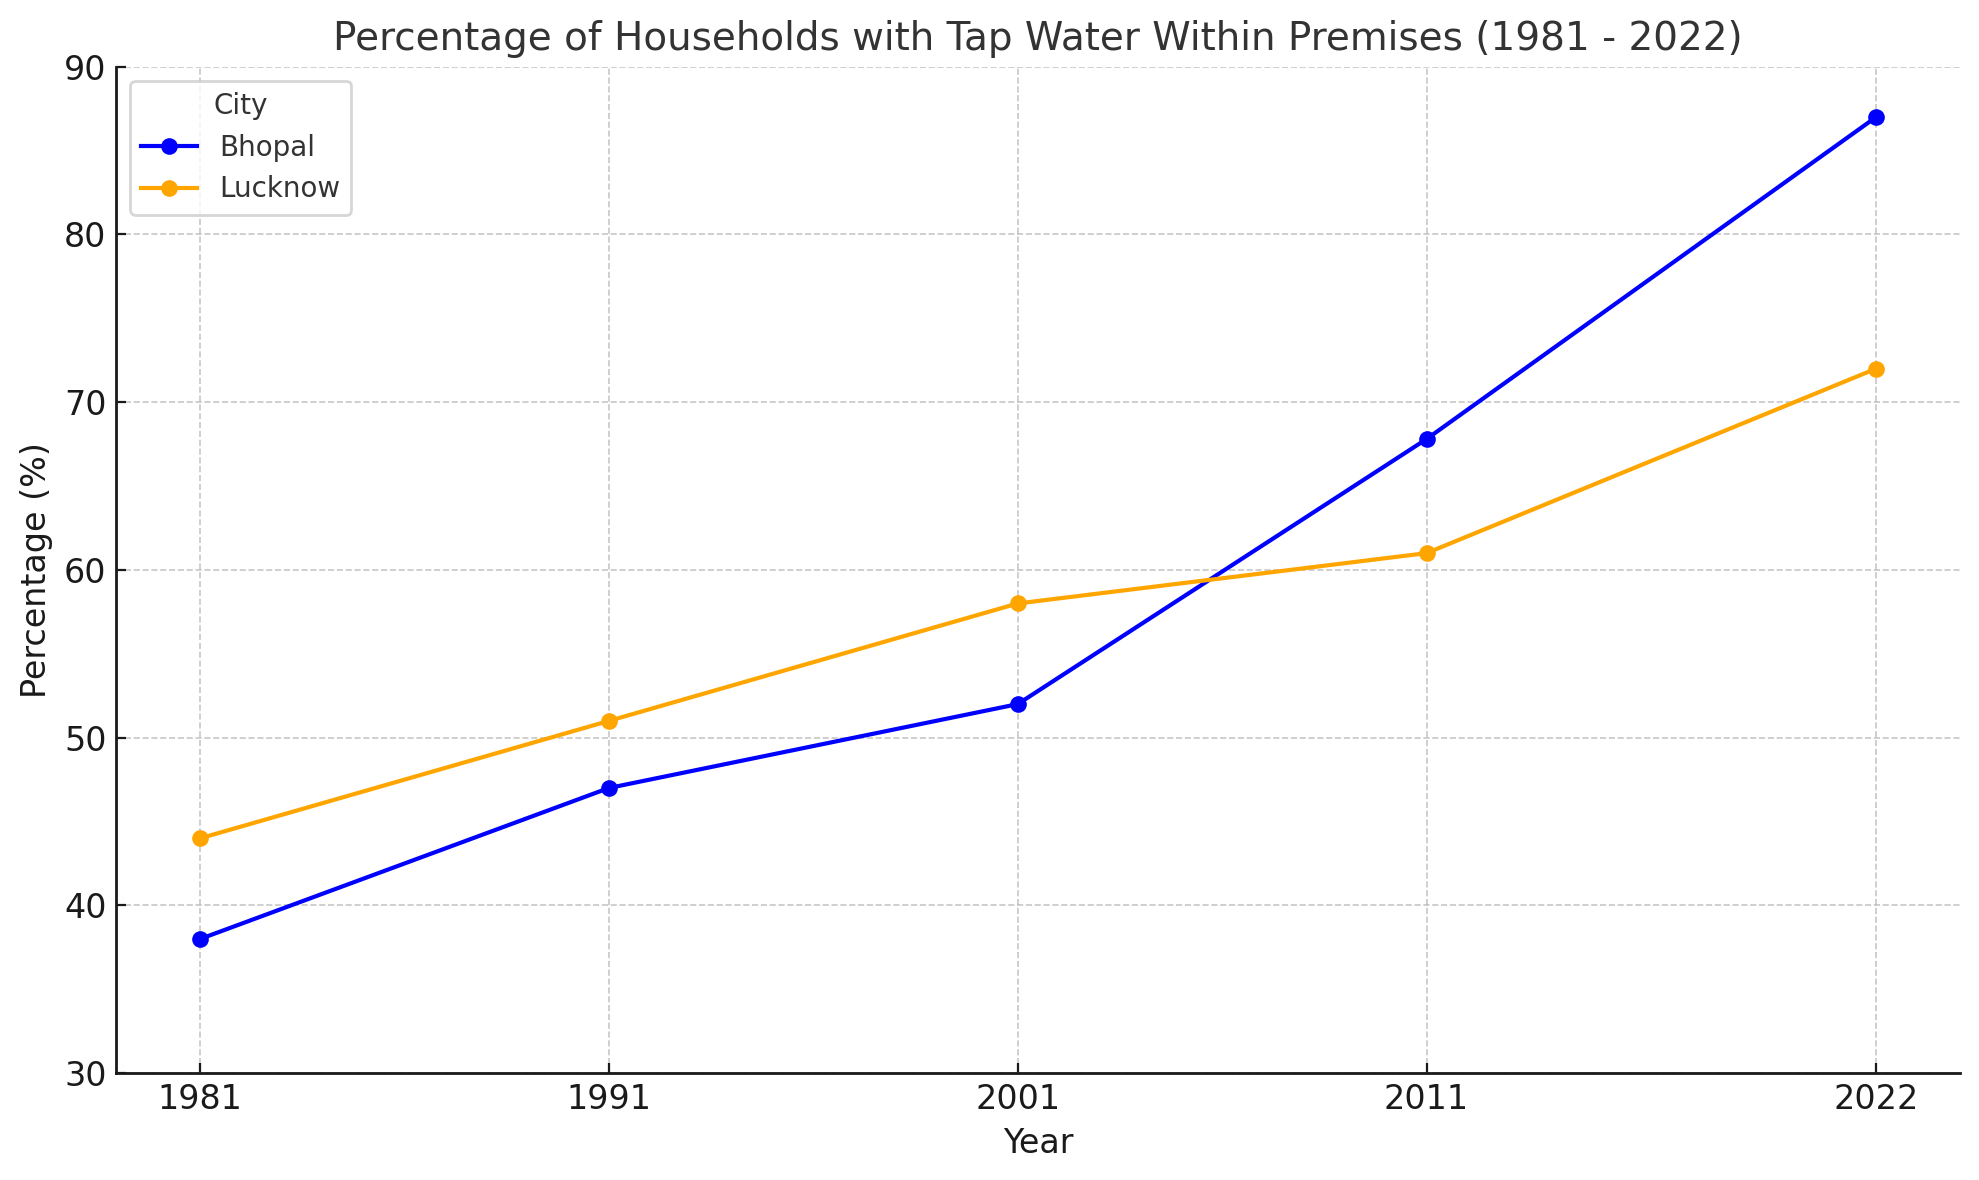
\includegraphics[width=.8\textwidth]{images/diff.png} % Adjust the width as needed
    \caption{Change in Tap water across Bhopal and Lucknow. Data for 1981-2011 is from the
Census of India, 2022 is from Primary Household Survey.}
   
\end{figure}

This chapter argues that the key determinant lies not in the formal characteristics of bureaucratic recruitment or tenure, but in how state-level bureaucrats mediate between political pressures and technical imperatives. These officials, positioned between elite policymakers and frontline implementers, play a crucial role in translating policy into practice. In Bhopal, state-level bureaucrats operated under what I term ``conditional autonomy" – sufficient operational independence to maintain technical standards while accommodating legitimate political demands. This enabled them to manage political-business relationships effectively, and legitimize community-driven solutions. The result was what I call "precarious universalism": broad service coverage that, while imperfect, proved more sustainable than alternative arrangements.

In contrast, Lucknow's water utility body, the Lucknow Jal Sansthan (LJS), remained trapped in what local officials describe as a ``\textit{Trishanku}-like" state – neither fully integrated into municipal governance nor granted meaningful autonomy. Despite having bureaucrats with similar professional backgrounds and protections as their Bhopal counterparts, LJS officials could not forge conditions for receiving  conditional autonomy necessary for effective service delivery. This resulted in persistent institutional paralysis, characterized by unresolved authority conflicts between state and city body, failed reform attempts, and reliance on informal, often inequitable solutions.

The comparative analysis reveals that successful service delivery depends not just on formal institutional designs, bureaucratic recruitment patterns, or resource allocation, but on bureaucrats' capacity to navigate complex political-administrative terrain. Where state-level officials can build coalitions, moderate competing interests, and institutionalize problem-solving routines, they create conditions conducive to improved service delivery – even without achieving ideal-type programmatic governance.

This argument advances our theoretical understanding of state capacity in three ways. First, it introduces the concept of \textit{conditional autonomy}, showing how bureaucrats can advance service delivery, even absent idealized Weberian conditions. Second, it highlights the distinct role of state-level bureaucrats as \textit{intermediaries within the state} apparatus, shifting focus from external brokers emphasized in previous research. Finally, it demonstrates how different forms of political-bureaucratic relationships produce varying service delivery outcomes, ranging from \textit{fragmentation to precarious universalism}.

The evidence presented comes from extensive fieldwork, including interviews with bureaucrats, politicians, and community leaders; analysis of administrative records; and a representative household survey comparing service access across both cities. This empirical foundation reveals how bureaucratic intermediation shapes not just project implementation but the broader patterns of urban service delivery, offering insights for understanding state capacity in developing contexts.


\section{Theory: Conditional Autonomy and Service Delivery}

Much of the literature on urban service provision frames governance in dichotomous terms: either programmatic policies delivered through impartial, rule-bound bureaucracies, or patronage-driven arrangements that reward political supporters \citep{pepinsky_bureaucracy_2017, kitschelt_patrons_2007-1}. In an idealized scenario, programmatic politics and autonomous bureaucracies would ensure predictable, universal access to public goods. Yet, across the Global South, such ideal types rarely materialize. Instead, cities more commonly exhibit hybrid conditions—arrangements that resist neat classification and combine elements of both programmatic and patronage-based governance.

Existing research acknowledges this hybridity. A robust body of work has explored the role of non-state intermediaries—brokers, party workers, and local leaders—who help citizens secure discrete, easily targeted goods like streetlights, ration cards, or communal water standposts\citep{auerbach_demanding_2019, krishna_politics_2007, pande_can_2011}. While these actors can alleviate immediate needs, their interventions often remain limited to small-scale, non-networked services. They rarely spur the coordinated, citywide improvements required by infrastructure-intensive public goods such as piped water or sewage systems. Moreover, dependence on these outside-the-state intermediaries can entrench fragmented patterns of provision, discouraging the state from assuming direct responsibility for long-term solutions. Thus, while brokers can deliver incremental benefits, they typically fail to foster comprehensive or equitable systems of public service delivery. Therefore, to understand how cities can achieve more stable and equitable outcomes, we must re-center the analysis on actors within the state -- specifically relationships between politicians and bureaucrats operating within formal government structures.


\subsubsection{Defining Conditional Autonomy}

By conditional autonomy, I refer to a configuration in which bureaucrats, embedded in political contexts rich in patronage and informal practices, secure a measure of professional discretion and normative standing, yet fall short of achieving the full institutional insulation or legal-rational coherence characterizing classic Weberian bureaucracies \citep{weber_max_1946, evans_government_1996}. In contrast to idealized portrayals of bureaucrats as uniformly rule-bound and shielded from political interference, conditional autonomy emerges amid ongoing negotiation and selective compromise between bureaucrats and political elites \citep{migdal_strong_1988, heller_labor_1991}. Key Features of Conditional Autonomy:

Partial Insulation:
Rather than being categorically free from political interference, bureaucrats maintain a circumscribed space for technical judgment. This partial insulation may derive from professional reputation, informal understandings, or the ability to leverage limited but salient points of resistance to politically motivated directives \citep{grindle_divergent_1997, tsai_accountability_2012}. Although not absolute, these forms of insulation temper capricious interventions and uphold minimal technical standards.

Strategic Adaptation:
Bureaucrats exercise agency through selective accommodation and resistance, strategically yielding on issues like incremental resource deployment or minor policy adjustments to safeguard core domains of technical integrity and long-term planning \citep{pepinsky_bureaucracy_2017, auerbach_clients_2019}. In doing so, they skillfully navigate a terrain of shifting alliances and informal deals, maintaining enough leeway to incrementally improve service delivery outcomes despite persistent patronage pressures.

Incremental Norm-Building:
Over time, the pragmatic engagements that constitute conditional autonomy help consolidate informal norms of professional conduct and create a shared understanding of acceptable interventions. Repeated bargaining episodes not only stabilize expectations but also generate incremental improvements in administrative routines, contributing to more predictable patterns of political-bureaucratic exchange \citep{levi_rule_1988, fukuyama_governance:_2016}.

Capacity Enhancement Under Constraint:
Conditional autonomy’s viability improves through modest but meaningful investments in administrative capacity, such as better data systems, procurement reforms, and targeted training. These measures enhance the bureaucracy’s credibility and negotiating power, enabling it to insist more effectively on technical standards when confronting political demands \citep{hawes_political-bureaucratic_2008, scott_seeing_1998}

In sum, conditional autonomy does not represent a stark departure from patronage-based politics, nor does it approximate a fully programmatic or “ideal-type” bureaucracy. Instead, it constitutes a negotiated, intermediate condition in which bureaucrats shape and reshape the boundaries of their discretion over time. This dynamic, iterative process allows even politically exposed bureaucracies to push large-scale, infrastructure-intensive projects toward broader, more reliable, and more equitable access—if not fully universal and programmatic, then at least more inclusive and durable than would prevail under unfettered patronage \citep{ hicken_building_2009}.

Visualizing these conditions (Table 1.1) along two axes—one for the nature of politics (ranging from programmatic to patronage) and another for bureaucracy (from autonomous to instrumental)—helps situate conditional autonomy in relation to other governance scenarios. At one extreme, fully programmatic politics and an autonomous bureaucracy yield coordinated, universal service provision, as seen in some European contexts. At the other extreme, patronage politics combined with an instrumentalized bureaucracy leads to collusion, producing fragmented, politically driven distribution of public services. In between these poles lie intermediate cases. Conditional autonomy emerges under patronage conditions when bureaucrats carve out limited but meaningful insulation, enabling them to shape service delivery more effectively, as exemplified by Bhopal. By contrast, collusion, as seen in Lucknow, reflects a situation where patronage pressures overwhelm any normative or technical constraints, resulting in persistent fragmentation.

\begin{table}[h!]
\centering
\caption{Relationship Between Bureaucracy and Politics}
\begin{tabular}{|c|c|c|c|}
\hline
\multicolumn{2}{|c|}{} & \multicolumn{2}{c|}{\textbf{Bureaucracy}} \\ \hline
\multicolumn{2}{|c|}{} & \textbf{Autonomy} & \textbf{Instrumental} \\ \hline
\multirow{4}{*}{\textbf{Politics}} & \textbf{Programmatic} & Coordinated & Dictatorship \\ 
& & (European Cities) & \\ \cline{2-4}
& \textbf{Patronage} & Conditional & Collusion \\ 
& & (Bhopal) & (Lucknow) \\ \hline
\end{tabular}
\caption*{}
\end{table}

The nature of the public good influences the relevance and impact of conditional autonomy (Figure 1.2).  For simple, easily targetable services—such as intermittent water standposts, streetlights, or periodic trash removal—both conditional autonomy and collusion can facilitate at least some form of delivery. Under collusion, these goods may be distributed as favors or political rewards (``localized patronage"). Under conditional autonomy, the same services become more evenly and reliably delivered, if not fully universa ``universalized delivery." However, for complex, networked infrastructure—such as piped water or integrated sewage systems—the distinction between conditional autonomy and collusion is more consequential. Conditional autonomy enables``precarious universalism”: broad coverage that remains imperfect and somewhat vulnerable, yet far better than the fragmented outcomes produced under collusion. Without a baseline of professional norms, capacity investments, and partial insulation from political meddling, complicated infrastructure projects cannot be sustained. Collusion in this realm generates``complete fragmentation,” with no stable, citywide solutions emerging and services delivered in a haphazard, inequitable manner. (see Figure 2).


\begin{figure}[H] % Use [H] to force the image to appear exactly where you place it
    \centering
    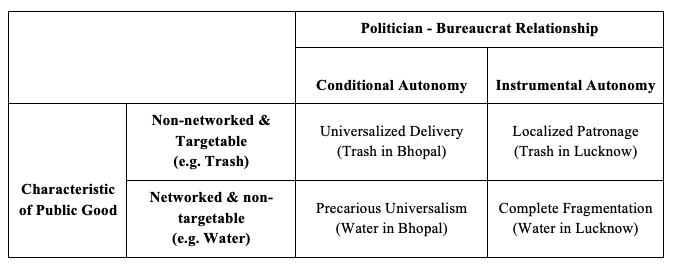
\includegraphics[width=.8\textwidth]{images/2by2new.png} % Adjust the width as needed
    \caption{Relationship between characteristic of Public Good and Politian-Bureaucrat Relationship}
   
\end{figure}

By highlighting conditional autonomy, this framework challenges the assumption that patronage and programmatic governance form a simple continuum. Patronage conditions do not preclude improvement. State-level bureaucrats, acting as intermediaries, can incrementally “upgrade” patronage systems by establishing professional norms, investing in capacity-building, and engaging politicians and contractors in strategic negotiations. In other words, conditional autonomy does not promise Weberian perfection, , but it can push systems toward more reliable and equitable service delivery than would be expected in a purely patronage-driven environment

The comparative cases of Bhopal and Lucknow illustrate these dynamics. Bhopal’s state-level bureaucrats secured a measure of conditional autonomy that facilitated citywide improvements in piped water access—albeit imperfect and precarious—while Lucknow’s collusive environment generated persistent fragmentation, stalled reforms, and reliance on informal arrangements. These empirical findings confirm that even in challenging political landscapes, conditional autonomy can help bureaucrats shepherd complex public goods projects closer to broad coverage and technical reliability.




\section{Institutional Paralysis \& Water Governance: The Case of Lucknow}

\subsection{Introduction}
The case of Lucknow vividly illustrates how institutional ambiguity and contested authority can obstruct coherent water service delivery. Here, the Jal Sansthan (LJS), formally tied to the municipal government but never truly integrated, occupies a precarious “\textit{Trishanku}-like” (twilight) state—nominally independent, yet effectively beholden to state-level agencies. As a result, each layer of authority pursued its own agenda, from state-level ministries resistant to local autonomy, to municipal officials constrained by financial instability, to LJS engineers lacking the power to implement technical solutions. Despite availability of finance and policy incentives, no credible intermediaries emerged to reconcile these divergent priorities. Instead of forging even minimal autonomy—such as localizing the Project Implementation Unit of a union government program or rationalizing water tariffs—politicians and bureaucrats gravitated toward short-term strategies, patronage-based arrangements, and fragmented service delivery. In theoretical terms, these dynamics align with the “collusion” scenario, where patronage politics and instrumentalized bureaucracies undermine attempts at structured, equitable solutions and trap institutions in persistent underperformance.


\subsection{Origins of Institutional Ambiguity: The Evolution of Lucknow City Water Utility}

\begin{quote} “Hum trishanku hai. Na idhar na udhar (We are in a twilight zone. Neither here nor there).”\footnote{Interview with the General Manager, Lucknow Jal Sansthan, Lucknow, 2022} 
\end{quote}

This was how the head of the Lucknow Jal Sansthan (LJS), Lucknow’s city-level water utility, described his institution’s predicament. Borrowed from a mythological king suspended between heaven and earth, the metaphor aptly conveys the LJS’s unsettled status.\footnote{In Hindu mythology, King Trishanku desired to enter heaven in his physical form. When the sage Vashishtha refused to help, Trishanku sought help from others, ultimately angering powerful figures and earning a curse. Attempts by Sage Vishwamitra to send him to heaven failed, leaving Trishanku suspended upside-down between earth and heaven. Determined, Vishwamitra created a new realm for him, and Trishanku remained there, eternally inverted. This tale birthed the phrase “Trishanku’s heaven,” denoting an unresolved, in-between state.} Formally tied to the city government yet never fully integrated, and nominally independent yet effectively beholden to external authorities, the LJS has failed to secure the operational coherence and autonomy envisioned when it was established in the mid-1970s. 

The Lucknow Jal Sansthan operates under a complex governance framework involving three distinct layers of control, each with its own priorities and limitations. (Figure 1):

At the highest level, the State Water Department maintains oversight through policy directives and funding decisions. However, with approximately 78\% of Uttar Pradesh's 241 million residents living in rural areas, the department's priorities and resources are heavily skewed toward rural needs. This imbalance is starkly reflected in the budget allocation: of the \$2 billion water budget, only \$241 million is designated for all urban utilities combined, with the remaining \$1.8 billion directed to rural areas. This distribution severely limits the resources available for urban infrastructure investment in cities like Lucknow.\footnote{PRS Legislative Research. (2021). \textit{Uttar Pradesh budget analysis 2021-22}. Retrieved from \url{https://prsindia.org/budgets/states/uttar-pradesh-budget-analysis-2021-22}} 

At the middle level, the Uttar Pradesh Jal Nigam (UPJN) serves as a parastatal authority responsible for technical standards, staffing decisions, and resource allocation across the state. As a body overseeing multiple urban centers, the UPJN treats Lucknow as just one of many clients, making it difficult to provide the focused attention and financial stability that the city's water utility requires.

At the local level, while the LJS is technically part of the Lucknow Municipal Corporation (LMC) following reforms implemented in 2009, this integration exists largely on paper. The LMC has limited real authority over the utility's financial or personnel matters. Although it theoretically has the power to set water tariffs, the LMC lacks the resources to fully incorporate LJS's operations. Further complicating this relationship, LJS staff members remain hesitant about deeper integration with the LMC, citing concerns about maintaining technical standards and stable payroll, particularly given the LMC's challenges in managing other services such as trash.

This tripartite arrangement leaves the LJS in a “Trishanku-like” state: formally linked to the city but effectively managed by higher-level bodies, financially dependent on state grants, and unable to carve out a coherent role for itself in local governance. To understand how these conditions emerged, we must examine the historical and structural choices that shaped Uttar Pradesh’s water governance institutions.

\begin{figure}[H] % Use [H] to force the image to appear exactly where you place it
    \centering
    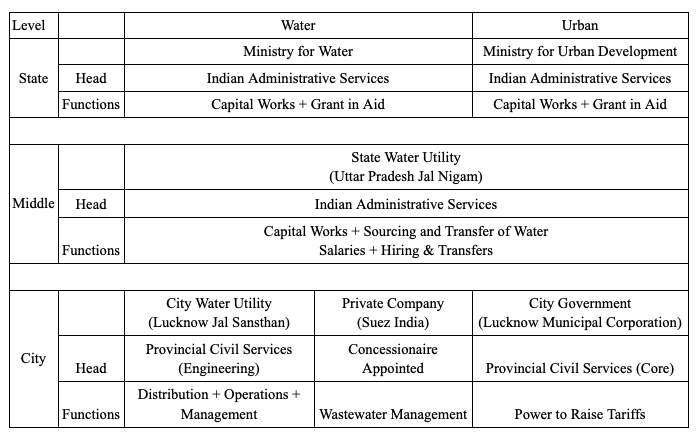
\includegraphics[width=1\textwidth]{images/Lwater.png} % Adjust the width as needed
    \caption{Administrative Institutions Governing Water Systems in Lucknow. Different Sources}
   
\end{figure}

Uttar Pradesh’s water sector modernization began in earnest in the 1970s, with international financial institutions—most notably the International Bank for Reconstruction and Development (IBRD), a precursor to the World Bank—offering funding and strategic guidance.\footnote{The Uttar Pradesh Water Supply and Sewerage Act, 1975 (Act 43 of 1975)}, Their core recommendation was to create specialized utilities capable of operating independently, raising their own revenues, and maintaining infrastructure without continuous state subsidies. Enacted in 1975, the Uttar Pradesh Water Supply and Sewerage Act established two new entities: the Uttar Pradesh Jal Nigam (UPJN) to oversee water management statewide, and city-level Jal Sansthans (including the LJS) to bring professional expertise and financial self-sufficiency to urban water provision.\footnote{During 1975–1990, the IBRD and the World Bank funded initiatives in “KAVAL towns” (Kanpur, Agra, Varanasi, Allahabad, and Lucknow) to test greater urban autonomy in water supply management.}

In theory, this arrangement promised a technical and managerial revolution. The Jal Sansthans were to operate like public utility companies, directed by expert general managers and supported by stable, tariff-based revenue streams. UPJN would coordinate larger projects and ensure statewide standards, while each Jal Sansthan would focus on local operations. In practice, however, these reforms never fully took root. Instead of forming distinct urban cadres or developing robust local revenue models, the Jal Sansthans remained administratively and financially tethered to UPJN and the State Water Department. Human resource reforms were neglected, and the same engineering cadres circulated among rural and urban postings, undermining the envisioned city-centric professionalism.\footnote{For a more detailed discussion read: India - Uttar Pradesh Water Supply and Sewerage Project (English). Washington, D.C. : World Bank Group. \protect\url{http://documents.worldbank.org/curated/en/979771468035977277/India-Uttar-Pradesh-Water-Supply-and-Sewerage-Project}}

\subsubsection{Persistent Rural Bias and Financial Constraints}

The skewed allocation of resources in Uttar Pradesh is crucial to understanding the LJS’s predicament. With 78\% of the population and pressing development needs located in rural areas, it is politically and administratively easier for state authorities to channel resources outside cities. This results in a systemic rural bias: rural sectors receive approximately \$9.62 per capita from the water budget, while urban residents must make do with about \$4.56 per capita.\footnote{PRS Legislative Research. (2021). \textit{Uttar Pradesh budget analysis 2021-22}. Retrieved from \url{https://prsindia.org/budgets/states/uttar-pradesh-budget-analysis-2021-22}} Although there may be developmental logic behind prioritizing rural areas—where farmers and low-income populations require immediate support—this imbalance starves urban utilities like the LJS of stable funding. Without adequate financial resources, LJS struggles to invest in trunk infrastructure or maintain existing networks, perpetuating weak service provision and low cost-recovery. The inability to generate sufficient revenue internally further cements its dependence on higher-level authorities.\footnote{See City Development Plan (pg. 18): \url{https://lmc.up.nic.in/pdf/nnfinal.pdf}; also World Bank South Asia Region Energy and Infrastructure Unit Report No. 27288 (2003).}

\subsubsection{Fragmented Staffing and Unstable Incentives}

The institutional complexity of Lucknow's water management system is deeply rooted in its workforce composition and leadership structure. The LJS and its parent organization, the Uttar Pradesh Jal Nigam (UPJN), are staffed by officers recruited through state-level engineering examinations. Senior officials come from the Combined State Engineering Services, while junior staff are selected through the Combined Junior Engineer Examination, collectively forming the Uttar Pradesh Engineering Services (UPES).

At the leadership level, the relationship between the UPES-cadre head of LJS and the UP Provincial Civil Services (UP-PCS) Commissioner of LMC has been marked by contention. Despite similar recruitment standards, these state officials operate under fundamentally different institutional frameworks. The UP-PCS officers manage broader administrative responsibilities and typically lead major state organizations like the LMC, while UPES officers maintain their specialized domain within water services, both in Lucknow and across the state.
The LMC's financial constraints also significantly influence this institutional relationship. From the LJS's perspective, deeper integration with the financially struggling LMC appears to offer little benefit while potentially adding bureaucratic complexity without improving their resource situation. Since funding and personnel transfers are managed at the state level rather than through Lucknow's municipal administration, the LJS has minimal incentive to subordinate itself to LMC oversight.

Field research reveals significant operational tensions, particularly among lower-level staff. Despite their formal subordination to the LMC, LJS employees strongly resist full integration, citing concerns about maintaining technical efficiency and professional autonomy(See figure 1.4). They frequently point to the LMC's challenges in managing solid waste—characterized by delayed salaries, procurement issues, and political interference in technical decisions—as a cautionary example of what might happen under complete municipal control.\footnote{Interview with the President, Uttar Pradesh Jalkal,Jalsansthan Adhikari/Karamchari Sanyukt Morcha, Lucknow 2021}
The state-wide transfer system for both engineering officers and staff creates additional complications. Many personnel prefer rural postings, which offer greater autonomy and control over resources, including more direct influence over infrastructure contracts and public works projects. In urban settings, these opportunities must be shared with the LMC, creating a less attractive professional environment. This preference for rural postings, combined with limited local institutional attachment and unclear advancement paths within the LJS, undermines staff commitment to addressing Lucknow's complex water management challenges.

\begin{figure}[H] % Use [H] to force the image to appear exactly where you place it
    \centering
    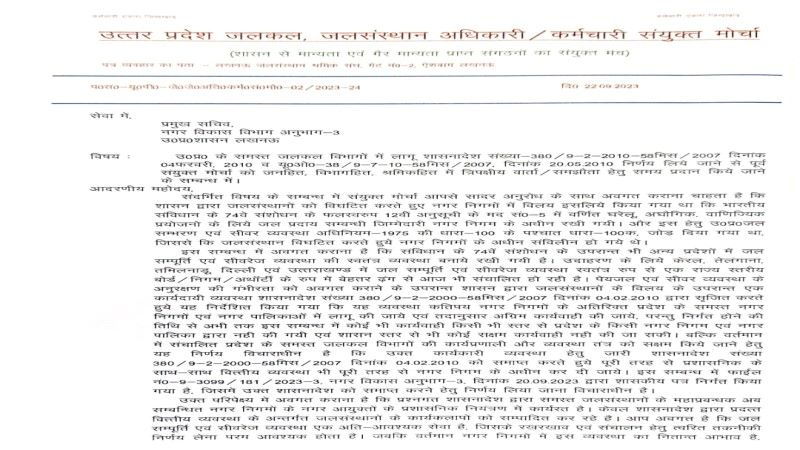
\includegraphics[width=1\textwidth]{images/पत्र-एक.jpg} % Adjust the width as needed
    \caption{Letter from the employee association against merger of the LJS with LMC, Lucknow 2023. Source: Primary Field Work}
   
\end{figure}

As a technically-oriented engineering organization, the LJS maintains a deliberate distance from political interfaces, operating through separate administrative offices distinct from the Lucknow Municipal Corporation's (LMC) facilities where political actors typically engage with municipal officials. While the LJS presents this separation as necessary to preserve technical autonomy and operational efficiency, this institutional arrangement has created problematic barriers to democratic accountability. The physical and organizational separation from political oversight has fostered an environment of bureaucratic insularity that diminishes responsiveness to public concerns. This disconnect is particularly evident in the experiences of elected officials within the LMC. These representatives, including municipal councilors, find themselves in an untenable position: they are the primary recipients of citizen grievances about water services yet lack effective mechanisms to influence LJS operations or demand improvements. As revealed in interviews, even the Mayor of Lucknow encounters significant difficulties in securing meetings with LJS officials, highlighting the extent of bureaucratic unresponsiveness.\footnote{Interview with Sanyukta Bhatia, Mayor of Lucknow Municipal Corporation from 2017-2023 }

The absence of robust oversight mechanisms and performance monitoring frameworks has allowed the LJS to operate with minimal public accountability. This institutional design, while potentially shielding technical operations from political interference, has ultimately contributed to persistent service delivery challenges that remain unaddressed due to the lack of effective channels for political and public oversight.

International agencies have tried to break these silos. External donors and consultants advocated for holistic reforms that would link water provisioning to broader urban development goals. For instance, they suggested using enhanced property tax revenues—administered by the LMC—to cross-subsidize water infrastructure managed by LJS. In theory, this approach could address LJS’s revenue shortfalls, reduce reliance on state grants, and foster greater integration between technical and administrative arms of the city. Yet these initiatives faltered. Each institution—UPJN, LJS, LMC—guarded its autonomy and prerogatives. Without a shared platform or credible enforcement mechanisms, negotiations stalled. The LMC lacked confidence in channeling scarce revenues into an entity it could not fully control, and LJS officers, mistrusting LMC’s fiscal instability, remained reluctant to recalibrate their internal procedures or accountability lines.
This persistent fragmentation prevented external interventions from catalyzing meaningful institutional change. Even when well-funded international programs offered opportunities for capacity-building and better financial planning, the entrenched patterns of isolation and resistance proved difficult to overcome. The LJS’s precarious position, lacking both proper autonomy and genuine integration, meant that it could not leverage external inputs effectively, and citywide strategies for improved service delivery remained unrealized.

In sum, the Lucknow Jal Sansthan’s enduring “Trishanku-like” condition emerges from a confluence of historical, institutional, and political factors. Intended as a technically autonomous utility, LJS instead became a hybrid entity, trapped among competing jurisdictions, weak revenue streams, and ambiguous lines of authority. The subsequent sections will show how this unsettled organizational landscape hinders coherent reforms, encouraging reliance on informal, short-term coping strategies rather than durable improvements in water delivery.




\subsection{Contested Authority: State Control versus Municipal Autonomy}

The institutional ambiguity and contested authority discussed above prevented Lucknow’s political and bureaucratic actors from reconciling their divergent priorities. As the city’s water challenges intensified, these misalignments solidified into persistent conflicts among state-level politicians, elite bureaucrats, and city-level officials in the LMC and LJS. Instead of devising a cohesive strategy, each faction pursued its own agenda, resulting in fragmented governance and inefficiency. Despite substantial external funding and reform incentives, such as those provided under JnNURM, these tensions meant that large-scale investments failed to produce lasting infrastructure improvements or reliable service delivery. Examining how these elite-level coordination failures shaped the water utility’s capacity thus illuminates the everyday realities of water access in Lucknow.

\subsubsection{\textbf{Differing Perspectives Among Stakeholders}
}
Elite state-level bureaucrats, particularly those in the Indian Administrative Service (IAS), consistently portrayed water as a foundational public good best managed through technical standards and centralized authority. One former Secretary of Water Resources emphasized the importance of professional insulation:

\begin{quote} "The real obstacle is not the availability of water—Uttar Pradesh has more than enough sources—but the inability to implement solutions free from local meddling. When every decision is subject to neighborhood-level demands and short-term political interests, you lose technical rigor and long-term vision. Keeping the system under state-level control ensures that engineering standards, not local pressures, guide the process. Only then can we achieve true efficiency and competence."\footnote{Interview with the Secretary, Department of Water Resources (2012-2018), Indian Administrative Services. Lucknow}
\end{quote}

For these technocrats, Uttar Pradesh’s abundant water was not scarce, but poorly managed. Insulating water governance from local political bargaining and relying on professional engineering cadres, in their view, provided the clearest path to maintaining quality, reliability, and fairness.

State-level politicians, however, often adopted an even more radical stance that rejected the commodification of water. Former Urban Development Minister Mohd. Azam Khan publicly opposed installing water meters—a measure intended to improve cost recovery and operational efficiency. In an interview, he justified this position

\begin{quote} “We have enough water. They [bureaucrats] used to tell me water rates needed to be increased… new meters need to be installed. I said use these funds to improve the drinking water supply infrastructure. People use water only as much as they need. They don’t waste any water. Actually, you are the ones who lose water.. Half of the water in Lucknow is lost during transmission. Surely, this is not people’s fault.”\footnote{Interview with Md. Azam Khan, Minister for Urban Development (2012-2017), Rampur Jail 2022.}

\end{quote}

While the minister acknowledged that low per capita incomes might limit consumers’ ability to pay, the primary critique targeted systemic inefficiencies—distribution losses, poor infrastructure, and unreliable quality—rather than consumer behavior. Official reports indicate that operational losses—primarily due to leakage, inefficient maintenance, and outdated infrastructure—consistently hover around 50\%, underscoring the entrenched inefficiencies that persist despite decades of policy interventions and attempted reforms (See table 1.2). Notably though, this stance was not mere electoral expediency; it represented a deeper ideological position on public service provision. Another Minister for Water Resources echoed similar sentiments, reflecting a stable ideological position rather than mere electoral pandering.\footnote{Same sentiment was repeated by Ashoka Kumar Dohre, Minister for Water Resources (2007-2011). Lucknow 2022, 2023.} For these state politicians, water was a non-negotiable right, and any talk of pricing or metering threatened to politicize the issue and alienate voters.

At the city level, however, the LMC—home to city bureaucrats and municipal politicians—saw matters differently. Municipal officials argued that local control over water utilities could improve responsiveness. “If we had them [LJS under LMC control], we would understand the city’s needs and serve more effectively,” explained one LMC Commissioner.\footnote{Interview with Commissioner, Lucknow Municipal Corporation (2022), UP Provincial Civil Services, Lucknow 2022} City-level politicians like municipal councilors also stressed that LJS engineers focused on technical parameters while ignoring the everyday realities of informal neighborhoods. “They do surveys and make estimates. We know the ground realities—our ears are to the ground, theirs are in the Secretariat,” lamented a former councilor.\footnote{Interview with Md. Saifullah, Councillor (2012-2017), Lucknow 2022} Yet city-level politicians and administrators recognized a harsh truth: the LMC lacked the financial muscle to absorb LJS fully. The former Mayor, Dinesh Sharma, conceded, “We simply do not have the funds to pay LJS employees… unless the state keeps providing grants.”\footnote{Interview with Dinesh Singh Sharma, Mayor (2006-2017), Minister for Urban Development (2017-2022), Lucknow 2021} 

Within the LJS itself, engineers and managers resented both local political meddling and the constraints imposed by state authorities. As one General Manager, the head of LJS explained:

\begin{quote}

 “We are stuck in a cycle: without adequate revenue, we cannot invest in infrastructure; without improved infrastructure, residents will not trust us enough to pay. Every time we try to break this loop—say, by proposing a tariff increase—either the state pushes back or local politicians object. It’s not that we don’t understand what needs to be done. We do. But without the authority to set rates, hire qualified staff, or control our own budgets, we’re forced to patch things up with short-term fixes. This isn’t about engineering anymore.”\footnote{Interview with General Manager, Lucknow Jal Sansthan (2013-2016). Lucknow 2023}\end{quote}

Their perspective was that without proper revenue mechanisms—such as rationalized tariffs and widespread metering—to generate the funds needed for infrastructure upgrades, the cycle of underinvestment, poor quality, and low trust would remain unbroken.

These divergent perspectives—state-level politicians wary of metering, top bureaucrats favoring centralized technical control, city officials seeking greater local authority, and LJS engineers advocating for revenue-generating mechanisms like metering—would not necessarily doom reform if credible intermediaries existed to align their interests. In many settings, political leaders or bureaucrats step forward to translate high-level mandates into workable arrangements; in others, civil society organizations outside the state persuade key actors to act. In Lucknow, however, such intermediation never materialized.

\begin{table}[h!]
\centering
\caption{Water Supply and Losses (2005-2019)}
\begin{tabular}{|p{1.5cm}|p{2.5cm}|p{2.5cm}|p{2cm}|p{3cm}|p{2.5cm}|}
\hline
\textbf{Year} & \textbf{River Water (MLD)} & \textbf{Ground (MLD)} & \textbf{Total (MLD)} & \textbf{HH with piped water (\%)} & \textbf{Losses (\%)} \\ \hline
2005 & 270 & 190 & 205 & 47\% & 53\% \\ \hline
2016 & 475 & 400 & 875 & 62\% & 30\% \\ \hline
2019 & 400 & 630 & 756 & 64\% & 45-50\% \\ \hline
\end{tabular}
\caption*{Source: City Development Plan, pg. 19-20. All figures supplied by Lucknow Jal Sansthan.}
\end{table}


A telling example comes from the scenario described by a civil society representative who observed the union government's program (Jawaharlalal Nehru National Urban Renewal Mission or JnNURM) implementation in Uttar Pradesh.\footnote{Under JnNURM: central government typically contributed 50\% of project costs, the state government 30\%, and the
city government 20\%. State and city governments often relied on organizations like the ADB, World Bank, DFID, or
USAID for their shares.} Each grant-receiving city was paired with an international agency offering capacity-building support—specialized consultants in human resources, finance, and governance—at no cost.\footnote{ For Lucknow this agency was US-AID which funded this project under the Financial Institutions Reform and Expansion–Debt and Infrastructure (FIRE-D)} The arrangement was intended to last the full duration of the ten-year funding period, a substantial opportunity for institutional strengthening. In mid-2007, as discussions arose over the placement of the Project Implementation Units (PIUs), as these capacity building offices were referred to, the city’s Municipal Commissioner proposed situating the PIU within local agencies. The Commissioner argued that doing so would improve coordination, allow responsive adjustments, and ensure that technical expertise guided daily operations. LJS officials also supported embedding consultants in their departments.

Yet, as the civil society representative recalled, the idea of placing the PIU in either the LMC or LJS was never seriously entertained. “Cities in UP were complete pushovers,”\footnote{Interview with the Member from Regional Center for Economic and Urban Studies, Lucknow. Lucknow 2021, 2022} she explained. “Secretaries would say, ‘Lucknow does one thing—garbage. They don’t need consultants for that.’” When she countered that the city’s limited capacity was precisely why the PIU was needed on-site, a senior bureaucrat offered a further rationale: “If Lucknow got the PIU, other cities would soon demand the same. We ourselves were starved of talent. In 2005, I had two computer operators for over five hundred urban local bodies. The hope was that centralizing expertise would eventually trickle down.” In the end, the PIUs were set up at the state secretariat (rebranded as Project Management Units or PMU). Over time, as fresh funding arrived in 2009, and again in 2011 and 2016, the question of relocating PIUs to the city reemerged, only to be rebuffed each time.

The inability of the LMC and LJS to secure the relocation of the PIU from state-level agencies to the city underscores the depth of their institutional constraints. Despite the PIU representing a relatively modest administrative reform, neither the LJS nor the LMC could successfully advocate for its placement within their organizations. This failure to secure even this small measure of autonomy revealed the extent of their institutional isolation and debilitation.

The state's refusal to relocate the PIU pointed to a more fundamental governance crisis. Lucknow's city-level bureaucrats found themselves in an impossible position: nominally responsible for water service delivery yet lacking the basic tools of administrative authority. While they had gained certain peripheral powers, such as tariff-setting authority, the state retained iron grip over all meaningful levers of control - staffing decisions, capital budgeting, and procurement authority. This arrangement left city officials unable to build the institutional credibility needed to advocate for greater autonomy.

The circular nature of this predicament proved particularly damaging. Without a track record of successful administration, city bureaucrats could not convince state authorities that localizing the PIU would enhance project governance. Yet without control over basic administrative functions, they could not develop the capabilities and safeguards that might have demonstrated their readiness for greater responsibility. State officials could always point to this lack of proven capacity to justify maintaining centralized control, perpetuating a cycle of institutional weakness that made meaningful reform increasingly difficult.

\subsubsection{Failed Reform and Institutional Stalemate}

This dynamic of mutual mistrust and restricted authority did not remain a theoretical concern; it materialized in the city’s encounters with national and international development programs. As discussed earlier, the PIU instead of operating locally, embedding specialized consultants in the LMC and LJS was placed in the Secretariat. These arrangements—tolerated by international agencies despite violating original contract terms—led to delays and growing dissatisfaction. Consultants noted that senior bureaucrats in Lucknow insisted the Secretariat (by which they meant the State government) was the only suitable locus of control.\footnote{Interview with RK Srinivasan, USAID Water, Sanitation and Hygiene Finance (WASH-FIN) Delhi 2023} Yet by excluding local politicians and the LJS from meaningful input, the state created a knowledge vacuum. Without LJS insights, critical decisions—such as whether to pursue comprehensive city-wide coverage or focus first on established urban cores—became contentious. The state-level utility favored newly incorporated areas like Gomti Nagar and Transport Nagar, anticipating modernization and better returns through user fee, while the LMC advocated improvements in older neighborhoods aligned with its political base.\footnote{Interview with Fire-D consultants in PMU Lucknow 2009-2012, Delhi 2023} The resultant stalemate was not merely technical but deeply political, revealing the institutional fault lines embedded in Lucknow’s water governance. In this, the LJS - the body which actually had to do the work had little or no say. 

The politicization of procurement compounded the problem. With the ruling Samajwadi Party favoring a Dubai-based firm and the BJP-led municipal government insisting on the lowest bidder, contractor selection controversies escalated.\footnote{Interview with SK Singh, PCS officer, Commissioner of Lucknow 2007-2012. Delhi 2023} Allegations surfaced that BJP leaders privately lobbied for companies tied to their party, including one owned by the son of a then-Member of Parliament.\footnote{ibid.}Such politicization and marginalization of local expertise eroded confidence in the reforms, and ultimately led to key international agencies reducing or withdrawing their support. Independent evaluators offered harsh assessments:

“In Uttar Pradesh, stakeholders noted very low capacity across the state and perennial recruitment challenges further complicated by the state government’s fragmented management and shifting directivess. Capacity to plan and execute development projects is weak, and Lucknow’s low-level staff capacity to manage finances and technology is limited. Although a state-run utility is functioning, it is not always timely or geared to meet the on ground implementation challenges.” \footnote{India Financial Institutions Reform and Expansion–Debt and Infrastructure Ex-Post Evaluation, WASH Ex-Post Evaluation Series—Water Communications and Knowledge Management (CKM) Project, September 2018.}

In short, the FIRE-D episode underscores how the city’s lack of autonomy, combined with deep-seated political and bureaucratic tensions, neutralized opportunities for meaningful institutional strengthening. The very tools designed to foster local capacity and guide incremental reform became instruments of centralization, reinforcing a status quo in which neither efficiency nor accountability could flourish. Instead of bridging the gap between grand policy visions and street-level implementation, these international interventions remained stranded at the top, divorced from the local knowledge and authority needed to translate reforms into tangible improvements.

This same pattern of misalignment and inertia manifested itself in another key arena: the debates over water pricing policy. Since the early 2000s, city-level politicians, engineers, and select bureaucrats had recognized that static or token-level water tariffs could not sustain investments in infrastructure, maintenance, and service improvements. Although formal records indicate multiple resolutions passed by the Lucknow Municipal Corporation (LMC) to rationalize water rates—most recently in 2019—these attempts consistently stalled.\footnote{Proceedings of the Lucknow Municipal Corporation. Accessed from the Archives of the Lucknow Nagar Nigam Record Room. Lucknow 2021,2023} The rationale for pushing new tariffs was simple: marginalized groups in informal settlements were already paying private suppliers at higher rates for unreliable service. If the city could guarantee better quality and more dependable supply, many residents, even the poor, might accept moderate user fees.\footnote{ibid}\footnote{Interview with Syed Yawar Hussain Reshu, Leader of the Opposition, Lucknow city corporation, Lucknow 2022}

Yet, as city officials weighed these options, they confronted an entrenched resistance at the state level. State level politicians opposed both tariff hikes and the introduction of metering. Even senior bureaucrats in the Water Ministry framed metering and tariffs as distractions from addressing deeper structural issues: massive leakages, deteriorating pipelines, and haphazard distribution networks. Rather than turning to pricing mechanisms, these state-level actors urged the LJS to improve operations first—a proposition that seemed paradoxical, since operational improvements required stable revenue streams the LJS did not have. Interviews with senior bureaucrats shed further light on this impasse. Even sympathetic IAS officers, who privately acknowledged the necessity of pricing reforms, found it impossible to shift political positions. As one IAS officer who served in multiple state departments recounted:

 \begin{quote}

 “We tried to make a case to the Minister, but we had pumped so much money under various schemes and nothing really improved on the fiscal side, so it was tough to convince anybody on issues of water tariff.”\footnote{Interview with IAS officer who served in Water, Finance, Rural and Urban Development Ministry and retired as Additional Chief Secretary, Government of Uttar Pradesh. Delhi and Lucknow 2021-2024} \end{quote}

In other words, earlier failures to produce tangible improvements had eroded the credibility of reform advocates. Without visible results to justify higher charges, political leaders feared public backlash and questioned why consumers should pay more for the same unreliable service. This climate of mistrust and reluctance to invest political capital in unpopular decisions undercut any hope of implementing rational tariffs.

Caught in the middle, the LJS struggled to reconcile these opposing pressures. Local officials understood that without adjusting tariffs and introducing metering, the utility would remain trapped in a cycle of poor revenue generation and underinvestment.

Despite this clarity, the proposed compromise—municipal funding for meters combined with state-financed capital works—collapsed under fundamental fiscal constraints. Limited pilot attempts to install meters in newer neighborhoods yielded negligible results, not only due to technical shortcomings but also because consumers had grown accustomed to flat rates and informal arrangements. By 2019, official reports showed that citywide metering remained a distant goal.\footnote{Office of the Principal Accountant General (General \& Social Sector Audit), Uttar Pradesh. (2016). Annual Technical Inspection Report on Urban Local Bodies for the Year Ended 31 March 2016 (p. 23, 24). Government of Uttar Pradesh.} Without usage-based billing or cost-reflective tariffs, operational costs continued to outstrip revenues, perpetuating dependence on state subsidies and informal coping strategies.

Compounding these fiscal challenges, corruption and inefficiencies in billing and collection practices eroded the system’s integrity. State audits, newspaper investigations, and vigilante raids by the state’s Vigilance Department uncovered patterns of underreported water usage, unauthorized amnesties granted to favored consumers, and the deliberate undervaluation of property sizes in affluent neighborhoods.\footnote{During fieldwork, it was observed that frequent allegations of bribery and “overlooking” large connections were reported in local dailies. The state’s Vigilance Department also conducted raids, uncovering assets of top LJS officials vastly disproportionate to their incomes. In one noted case, a UP Jal Nigam employee possessed assets worth over \$4.8 million USD, far exceeding legitimate earnings.}

These malpractices illuminated the perverse incentives sustaining the status quo. Local politicians sometimes colluded with LJS field officers to supply discounted tanker water to informal settlements in exchange for under-the-table payments. Such arrangements, while offering short-term relief, entrenched patronage networks and discouraged systematic reforms. Both LJS staff and municipal officials privately acknowledged these informal workarounds as a symptom of a governance environment dominated by immediate political pressures rather than long-term strategic planning.

These governance fractures and political deadlocks carried significant fiscal consequences. Without rationalized tariffs or effective metering, the LJS forewent substantial revenue (estimated around  \$40.1 million) due to its inability to secure effective local management structures and coherent intermediation that could have financed infrastructural improvements and operational reforms. Earlier coordination failures, including missteps in project site selection and the failure to integrate external capacity-building measures, had already diminished the city’s access to critical development funding. An independent end-of-project appraisal underscored the gravity of these shortcomings: “No studies have been undertaken to assess the impact of subsidies on water supply, sewerage, and waste management services. Coverage remains at only 62\%, and bulk meters at source and distribution points are yet to be installed. Interdepartmental coordination between Jal Nigam, Jalkal, and LNN remains weak, hampering service quality and the feasibility of user charges. Full integration and a formal inter-governmental mechanism for coordination are still lacking.”\footnote{CRISIL Risk and Infrastructure Solutions Limited. (2014). \textit{Reform Appraisal Report – UIG: Uttar Pradesh – Package 3}. Mission Directorate, Jawaharlal Nehru National Urban Renewal Mission (JNNURM), Ministry of Urban Development. Retrieved from \url{https://localbodies.up.nic.in/CRISIL\%20REPORTS/UIG.pdf}, p. 73.}

In theory, JnNURM-linked reforms and legislative amendments should have broadened local autonomy and improved institutional coherence. Instead, they produced what organizational theorists term “myths and ceremonies” \citep{meyer_institutionalized_1977}—formal compliance with reform conditions, but scant substantive change. This disconnect became starkly evident in two critical arenas: the placement and operation of externally funded capacity-building programs, and efforts to rationalize water tariffs.

As a result, international agencies’ stipulations for a city-level PIU were met only in form, not in substance, and the intended capacity-building benefits never materialized. These arrangements—tolerated by international donors despite violating original contract terms—led to delays and mounting dissatisfaction. Consultants noted that senior bureaucrats in Lucknow insisted the Secretariat was the only suitable place for control.\footnote{Interview with RK Srinivasan, USAID Water, Sanitation and Hygiene Finance (WASH-FIN) Delhi 2023} Yet excluding local politicians and the LJS from meaningful input created a knowledge vacuum. Without the LJS’s insights, critical decisions—such as whether to target comprehensive citywide coverage or begin with established urban cores—were contentious. The state-level utility favored newly incorporated areas like Gomti Nagar and Transport Nagar, anticipating modernization and better returns through user fees, while the LMC pressed for improvements in older neighborhoods aligned with its political base.\footnote{Interview with FIRE-D consultants in PIU Lucknow 2009-2012, Delhi 2023} This stalemate was not merely technical but deeply political, revealing the institutional fault lines embedded in Lucknow’s water governance. Throughout this process, the LJS—the entity ultimately responsible for carrying out the work—was relegated to the sidelines, its expertise and local knowledge overshadowed by top-down dictates.

Procurement politicization further complicated the reforms. With the ruling Samajwadi Party favoring a Dubai-based firm and the BJP-led municipal government insisting on the lowest bidder, contractor selection controversies escalated.\footnote{Interview with SK Singh, PCS officer, Commissioner of Lucknow 2007-2012. Delhi 2023} Allegations soon surfaced that BJP leaders privately lobbied for companies tied to their party, including one owned by the son of a then-Member of Parliament.\footnote{ibid.} Such politicization fueled mistrust, undermining the credibility of reforms. The minister overseeing the project (currently serving jail time on corruption charges related to these initiatives)\footnote{Jal Nigam recruitment scam: \textbackslash{}url\{https://hindi.news18.com/news/uttar-pradesh/lucknow-jal-nigam-recruitment-scam-sit-submits-report-seeks-permission-to-register-fir-against-azam-khan-1355416.html} openly dismissed international partners, telling me:

\begin{quote} “The international partners were not important; they put undue pressure to bring their own people and agencies, but we did not think that way.” \end{quote}

This cavalier attitude eroded confidence and magnified doubts about the reforms’ integrity. Ultimately, misaligned incentives, political meddling, and institutional skepticism prompted key international agencies to withdraw support. The World Bank halved its commitment; USAID’s FIRE-D program also exited after disagreements over project direction.\footnote{Interview with RK Srinivasan, USAID Water, Sanitation and Hygiene Finance (WASH-FIN) Delhi 2023} In the project evaluation reports, independent auditors offered harsh assessments:

\begin{quote} “In Uttar Pradesh, stakeholders noted very low capacity across the state and perennial recruitment challenges further complicated by the state government’s fragmented management and shifting directives. Capacity to plan and execute development projects is weak, and Lucknow’s low-level staff capacity to manage finances and technology is limited. Although a state-run utility is functioning, it is not always timely or geared to meet on-the-ground implementation challenges.”\footnote{India Financial Institutions Reform and Expansion–Debt and Infrastructure Ex-Post Evaluation, WASH Ex-Post Evaluation Series—Water Communications and Knowledge Management (CKM) Project, September 2018.} \end{quote}

Nominal reforms and promised international funding—intended to bolster local capacity and professionalize the LJS—therefore yielded scant results. Instead of enabling conditional autonomy or cultivating a capable local bureaucracy, the PIU arrangement became a top-down tool reinforcing state-level dominance. Centralized decision-making and entrenched mistrust neutralized external expertise and stifled long-term planning. Without clearly defined authority lines between state and municipal actors, Lucknow’s water governance remained an institutional void, offering neither the efficiency gains of a more autonomous bureaucracy nor the accountability of genuinely devolved authority.

To summarize, In the first section, the analysis focused on how the Lucknow Jal Sansthan (LJS) found itself trapped in institutional limbo—formally anchored to the city government but never truly integrated, and ostensibly under state authority yet lacking genuine autonomy. In this subsequent exploration of elite coordination failures, it became clear that neither city-level actors nor their state-level counterparts could overcome the deep-rooted mistrust and entrenched interests that thwarted effective policy implementation. Despite considerable external funding and policy incentives, no credible intermediaries emerged to reconcile divergent priorities and to build a more coherent governance structure. Instead of securing even modest autonomy—such as locating the PIU at the municipal level—or rallying behind incremental reforms like tariff adjustments, the city’s politicians and bureaucrats resorted to short-term political strategies and patronage, while state bureaucrats and politicians refused to relinquish meaningful control. This dynamic encapsulates what the theoretical framework characterizes as “collusion,” wherein patronage politics and instrumentalized bureaucracies lock institutions into a cycle of fragmentation and underperformance, ultimately denying the city and its residents the potential gains of more efficient, equitable, and sustainable water service delivery.


\subsection{ Emergence of Hybrid Solutions: Local Adaptations and Their Consequences}

The previous section illustrated how elite-level efforts to coordinate Lucknow’s water governance fell short, with state and city authorities locked in distrust and fragmented policymaking. Yet the demand for water did not simply evaporate. Under conditions of top-level fragmentation, local-level actors—frontline LJS staff, councilors, petty contractors, and neighborhood intermediaries—stepped in, relying on borewells, handpumps, and tubewells to fill service gaps. My field observations and interviews indicate that these stakeholders felt compelled to provide some tangible relief, however improvised or ad hoc. Rather than delivering stable, inclusive solutions, however, this bottom-up improvisation took the form of collusion—tacit, informal agreements that perpetuated selective gains, entrenched inequalities, and ultimately mirrored the very dysfunctions that plagued coordination at higher levels.



Despite official claims of increased coverage, a persistent gap remained. Various sources offered differing statistics: a 2019 government report suggested 62\% piped access, the LJS later claimed 80\% by 2022, but a citizen survey conducted co-terminus with this dissertation found only 72\% reported access (Table 1.3). Regardless of the exact figure, about 25–30\% of Lucknow’s population still lacked formal piped water. This widespread reliance on borewells, handpumps, and private arrangements—even among wealthier colonies—revealed a city-wide pattern:  even those with resources and political connections found it necessary to circumvent formal systems (Table 1.4). The absence of elite-level agreement had thus pushed the burden of ensuring basic access down to the local scale.

\begin{table}[ht]
\centering
\renewcommand{\arraystretch}{1.5} % Adjust row height
\setlength{\tabcolsep}{8pt} % Adjust column spacing
\begin{tabular}{|p{5cm}|c|c|}
\hline
\textbf{Source of Water} & \textbf{Bhopal (\%)} & \textbf{Lucknow (\%)} \\ \hline
Tap (Piped) & 86.11 & 72 \\ \hline
Borewell + Hand pump & 12 & 26 \\ \hline
Other sources & 2 & 2 \\ \hline
\multicolumn{3}{l}{\textit{Source: Primary survey under the Brown - India Citizenship Project 2022}} \\ % Add source note
\end{tabular}
\caption{Source of Water by City}
\label{tab:water_sources}
\end{table}

\begin{table}[ht]
\centering
\renewcommand{\arraystretch}{1.3} % Adjust row height
\setlength{\tabcolsep}{5pt} % Adjust column spacing
\begin{tabular}{|p{3cm}|p{3cm}|p{2.5cm}|p{3cm}|p{3cm}|}
\hline
\textbf{City} & \textbf{Housing Type} & \textbf{Tap (Piped)} (\%) & \textbf{Borewell + Hand Pump} (\%) & \textbf{Other Sources} (\%) \\ \hline
Bhopal & Shack          & 93 & 1  & 6  \\ \hline
       & Slum           & 97 & 2  & 1  \\ \cline{2-5}
       & Middle Class    & 87 & 12 & 1  \\ \cline{2-5}
       & Upper Middle    & 82 & 15 & 3  \\ \cline{2-5}
       & Rich            & 80 & 20 & 0  \\ \hline
Lucknow & Shack         & 48 & 37 & 15 \\ \hline
        & Slum          & 64 & 32 & 4  \\ \cline{2-5}
        & Middle Class   & 74 & 25 & 1  \\ \cline{2-5}
        & Upper Middle   & 71 & 29 & 0  \\ \cline{2-5}
        & Rich           & 78 & 21 & 1  \\ \hline
\multicolumn{5}{l}{\textit{Source: Primary survey under the Brown - India Citizenship Project 2022}} \\ % Add source note
\end{tabular}

\caption{Source of Water by City and Housing Type}
\label{tab:water_by_housing}
\end{table}

\vspace{2mm}


Groundwater extraction became the cornerstone of Lucknow’s de facto supply system (Table 1.5). The LJS maintained some 720 borewells, accounting for 25\% of the city’s groundwater draw, but a staggering one hundred fifty thousand (1.5 lakhs) privately managed wells contributed another 36\%.\citep{foster_lucknow_2009} Together, this decentralized infrastructure accounted for 99\% of total water extraction. This “solution” came at a high environmental and public health cost: the city earned an “over-exploited” classification for groundwater, and quality analyses frequently detected fluoride, arsenic, and fecal coliform contamination \citep{sinha_state_2021}.


\begin{table}[h!]
\centering
\caption{Groundwater Extraction in Lucknow}
\begin{tabular}{|p{4.5cm}|p{3cm}|p{4cm}|}
\hline
\textbf{Institution} & \textbf{Tube/Bore Wells (Units)} & \textbf{Tentative Ground Water Extraction (MLD)} \\ \hline
Lucknow Jal Sansthan (Borewells) & 720 & 356 \\ \hline
Private (Borewells, Tubewells, Handpumps, Submersibles) & 150,930 & 510 \\ \hline
Others & 640 & 533 \\ \hline
\textbf{Total} & \textbf{152,290} & \textbf{1,399} \\ \hline
\end{tabular}
\caption*{Source: Lucknow Jal Sansthan as mentioned in \citep{sinha_state_2021} }
\end{table}

As my fieldwork in Transport Nagar illustrates, informal settlements evolving on the city’s periphery navigated a dense web of political patronage and makeshift engineering. In informal settlements like Gindan Khera or Amausi, which emerged amid rapid urbanization and airport expansion, such hybrid provisioning became a necessity.\footnote{In Lucknow, the legality of a neighborhood significantly impacts residents' access to water services. However, this relationship is not a simple binary, as the type and location of the neighborhood also play a critical role. Illegal colonies near formal neighborhoods, particularly in the city's core, often have access to water connections due to a "spillover" effect. In contrast, residents of informal settlements like Transport Nagar rely on personal connections to local politicians or bureaucrats to secure water access. Obtaining a water connection is complicated by the fact that the Lucknow Municipal Corporation (LMC) grants No Objection Certificates (NOCs) for water, while the Lucknow Development Authority (LDA) determines land legality. This disconnect allows for discretion in granting NOCs, favoring those with the right connections. In affluent areas like Gomti Nagar, even residents of LDA-designated illegal colonies rarely face barriers to water access, unlike in Transport Nagar, where personal networks are more decisive. The complex interplay of legal, spatial, and social factors in shaping water access in Lucknow necessitates a nuanced understanding of water governance and citizenship that goes beyond simple binaries of legal/illegal and served/unserved.} Initially reliant on scattered hand pumps or distant public taps, these communities found that as the water table fell in the 1990s, a single tubewell managed by a local politician’s associates only partially eased the crisis. Soon, multiple private tubewells sprang up, charging residents INR 150–200 per month for thrice-weekly supply.\footnote{Field interviews, 2021,2022 }As the city densified, local MLAs and councilors leveraged their influence to install government-funded borewells or negotiate tanker deliveries. The result was a deeply politicized patchwork where gaining access often depended on personal connections, bribes, or being part of the councillors core support base. This qualitative finding is further reflected in the primary survey, which is representative of the city-level conditions in Bhopal and Lucknow (n=3,754). A full treatment of this is provided in Chapter 2, where I demonstrate empirically that knowing a politician personally increases the likelihood of receiving water services in Lucknow by 88.2 percentage points. This finding underscores that access to essential services is not merely anecdotal but systematically tied to political connections, as evidenced at the pan-city level. (See annexure for discussion of the key findings from the survey).

In Gindan Khera, for example, residents I interviewed described lining up for water from a community standpost only once or twice a week. When supply finally arrived—frequently at unpredictable hours, sometimes at dawn—they rushed to fill buckets and containers as quickly as possible. Those without personal connections to the local councilor’s aide or the borewell manager found themselves waiting longer or receiving less. Some residents admitted paying small “gifts” to the pradhan or the local party worker to secure water, particularly during the summer month and monsoon when ground water dried up or was laden with silt and impurities. One woman lamented, “If you don’t show your face at the councilor’s office or keep good relations with the pump operator, your household might end up with less water that week.” Another resident noted that wealthier neighbors sometimes negotiated private tanker deliveries, leaving poorer households to scramble for whatever trickled down. This was water access through informal patronage, not a stable public service.


\begin{figure}[H] % Use [H] to force the image to appear exactly where you place it
    \centering
    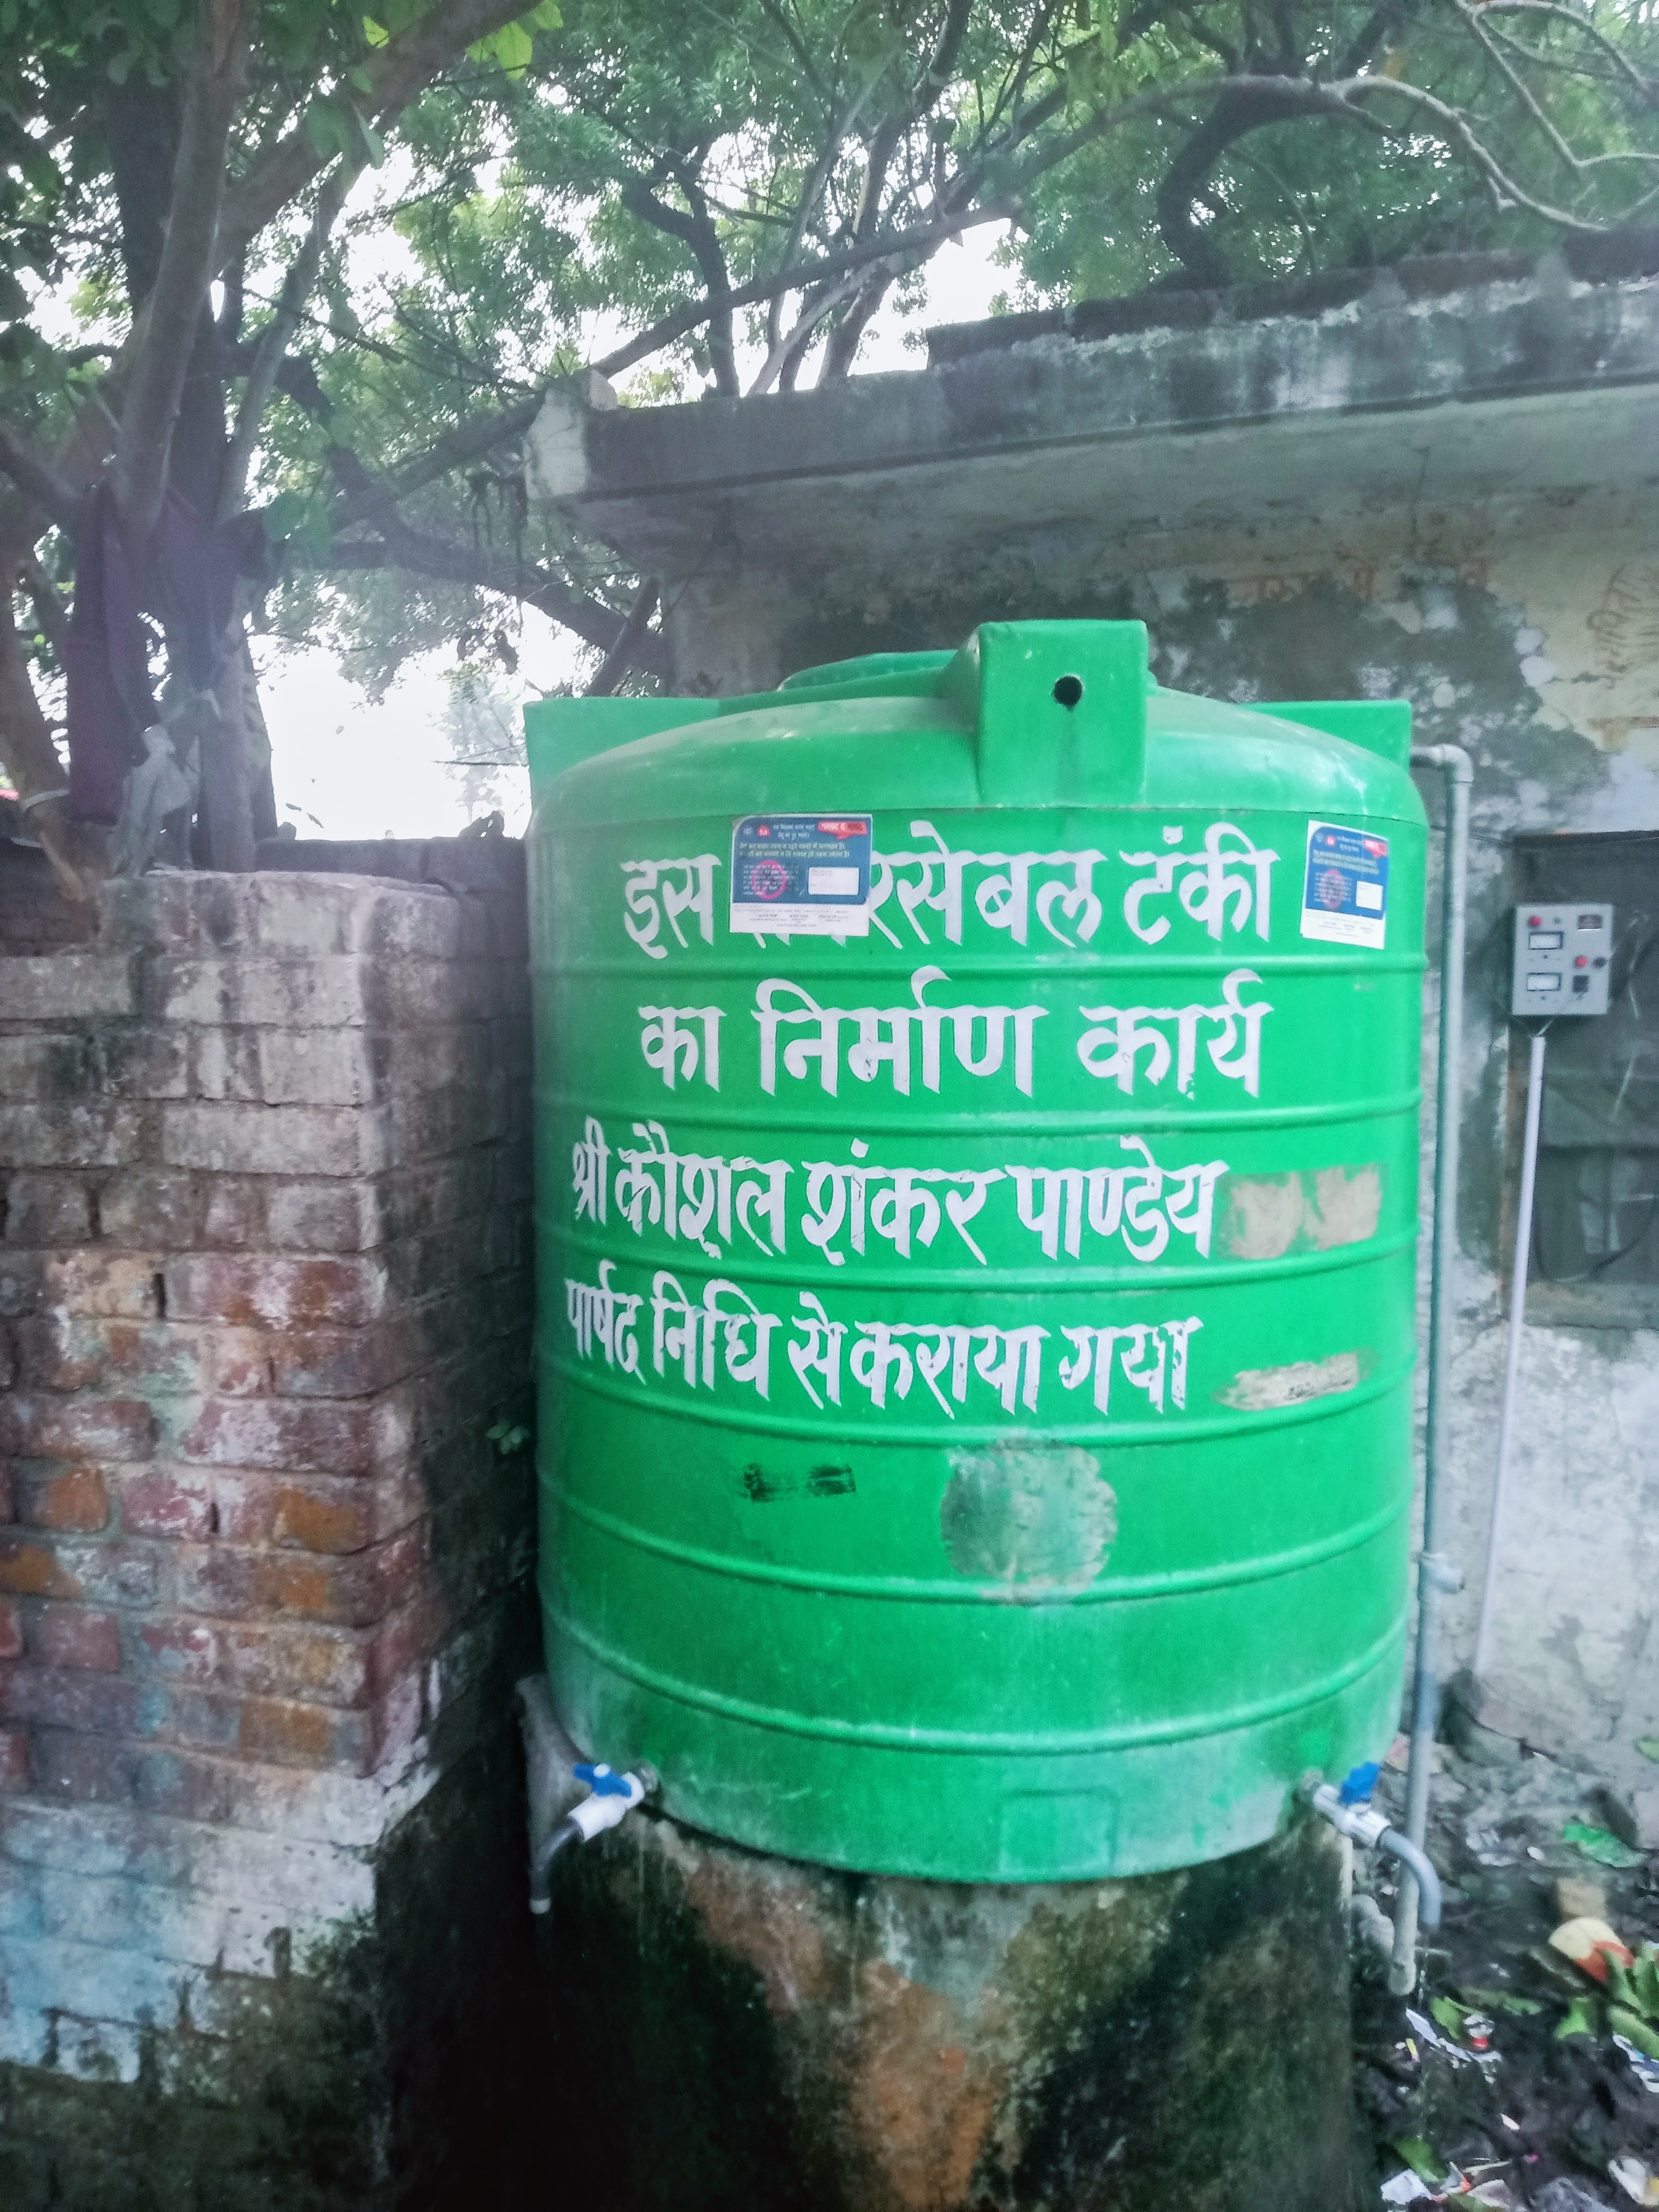
\includegraphics[width=.5\textwidth]{images/2by2.jpg} % Adjust the width as needed
    \caption{A submersible pump and tank installed by the ward councilor in Gindan Khera. Lucknow 2022}
   
\end{figure}


Securing even a single tubewell underscored the intricate coordination required at the grassroots level. Councilors responding to constituent demands petitioned the LJS for technical approvals and tendering, while the LMC, managing finances, often tapped councilors’ development funds and its own limited budget. The Sub-District Magistrate provided legal and administrative oversight.\footnote{Interview with LJS and Ward Councillors of Lucknow Municipal Corporation, Lucknow  2021 2022.} Within these negotiations, the LJS prioritized engineering standards and tendering, the LMC struggled to allocate scarce financial resources effectively, and councilors leveraged political influence to determine tubewell locations and managers. Installation costs ranged from INR 2.8 to INR 3.3 lakh, requiring multiple funding sources. \footnote{Interview with officials from the Public Health and Engineering Department, Government of Uttar Pradesh, Lucknow 2022}Between 2014 and 2022, the number of tubewells in Transport Nagar ward grew from three to eighteen, illustrating how quickly these improvised infrastructures could expand.\footnote{LJS records and interview with councilor of the Ward}

Such local-level coordination did represent a form of problem-solving absent at the top. Frontline bureaucrats and local politicians recognized that citizens could not wait for the LJS, LMC, and state to resolve their long-standing disputes. They had to deliver something, however meager or ad hoc. This reality explains why borewells proliferated and why local political actors invested in minimal fixes: they faced daily pressure from constituents who demanded water for cooking, cleaning, and basic sanitation. In these encounters, local actors could not rely on abstract references to bureaucratic gridlock. Instead, they provided what was immediately feasible—patchy, low-quality water—trading short-term relief for the possibility of long-term reform. This dynamic allowed local figures to claim credit and maintain political support, even though the solutions were inherently precarious and often exploitative.

Over time, what began as a coping strategy to circumvent elite-level deadlock hardened into a landscape defined by decentralized, small-group management. Installing tubewells and borewells required upfront investments and connections, which favored households and neighborhoods with political ties or financial resources. Less advantaged residents struggled with intermittent supply and poor-quality water, reinforcing existing inequalities. This environment incentivized no one—neither political leaders, frontline bureaucrats, nor private intermediaries—to push for a more coherent, programmatic water utility. The informal arrangements became entrenched, normalizing a culture of patronage, selective distribution, and periodic inducements rather than stable policy and reliable infrastructure.

In sum, the emergence of these hybrid solutions highlights the consequences of failed elite-level coordination. While top-level actors remained at odds, local stakeholders improvised a patchwork system that provided some water to most people but at the cost of equity, predictability, and public health. This bottom-up coordination, born of necessity rather than strategic design, did not foster conditional autonomy or set the stage for long-term improvements. Instead, it locked Lucknow into a suboptimal equilibrium: fragmented at the top, precariously adaptive at the bottom, and unable to overcome the structural barriers that made comprehensive reform so elusive.

As we move toward the conclusion of this chapter, the story of Lucknow’s water governance underscores that without effective bureaucratic intermediation to navigate complex political landscapes, even well-intentioned reforms and resource inputs cannot transcend fragmentation. The local stopgaps were a testament to human ingenuity and political responsiveness under duress, but they also starkly illustrated the limitations of governance models that fail to achieve even minimal conditions of autonomy and coherence.

\subsubsection{Conclusion}

Lucknow’s water governance reveals a complex interplay of institutional ambiguity, elite coordination failures, and fragmented local adaptations that have locked the city into persistently suboptimal outcomes. The LJS’s “Trishanku-like” position—formally tied to the municipality yet never fully integrated, technically oriented yet financially and administratively tethered to higher-level authorities—embodies a state of chronic uncertainty. At the elite level, state ministries, municipal authorities, and LJS officials struggled to align their interests or establish even minimal autonomy, leaving attempts at significant reforms—such as localizing the PIU or rationalizing tariffs—perpetually stalled. In the absence of credible intermediaries to forge consensus, local stakeholders stepped in with improvised, patronage-driven solutions that, while temporarily alleviating immediate needs, entrenched inequalities and circumvented the formation of durable, programmatic arrangements. This pattern aligns with what the theoretical framework terms “collusion”: a governance outcome in which patronage and fragmented authority replace any sustained, coherent effort to improve service delivery.

The enduring nature of these problems poses a deeper intellectual puzzle. International organizations like the World Bank have been engaged since the 1970s, directing substantial funding and offering strategic guidance aimed at strengthening institutions and enhancing capacity. Yet, more than half a century later, the fundamental weaknesses of institutional ambiguity, mistrust, and opportunistic local deals remain intact. This long history of repeated interventions, met with limited transformative change, suggests that technical fixes and incremental reforms, while necessary, cannot by themselves overcome the ingrained political and structural constraints that produce and sustain collusion. Without mechanisms to reconcile political demands, bureaucratic mandates, and technical imperatives, even decades of international support cannot guarantee a transition from fragmented, collusive arrangements to a genuinely integrated, equitable, and sustainable water governance system.

\section{Crafting Conditional Autonomy in Water Governance: The Case of Bhopal}

\subsection{Introduction}

Bhopal’s experience demonstrates that even in patronage-influenced environments and under significant structural constraints, skilled bureaucratic intermediation can foster a form of conditional autonomy—an institutional middle ground distinct from both idealized Weberian bureaucracy and purely instrumental arrangements. Unlike Lucknow, which remained trapped in a “twilight” condition of fragmentation, Bhopal found a path to “precarious universalism,” securing broad service coverage despite limited finances, political interference, and infrastructural challenges. This contrast underscores the central theoretical argument: complex public goods like piped water can be governed more effectively when bureaucrats operate as \textit{intermediaries within the state} and, crucially, \textit{outside the state}, bridging gaps between elite officers, frontline workers, political leaders, local businesses, and civil society.

In theory, developing-world cities often fail to achieve fully programmatic service delivery due to entrenched patronage politics and weak bureaucratic structures. Conventional accounts suggest two options: strive for Weberian autonomy or accept instrumentalized bureaucracies serving political ends. Yet Bhopal illustrates a third possibility. By embedding a Project Implementation Unit (PIU) directly into the municipal administration, the city empowered state-level bureaucrats to adapt incrementally. These officials, distinct from elite Indian Administrative Services (IAS) officers with short tenures, developed long-term urban expertise and relational capital. Rather than attempting to fully insulate administration from politics, they learned to navigate the pressures, expectations, and constraints of patronage while still maintaining technical standards and pursuing incremental reforms.

This conditional autonomy did not eliminate rent-seeking or political meddling, but it contained and structured these influences, allowing projects to move forward. State-level bureaucrats negotiated compromises, subdivided large initiatives into manageable parts, and balanced the demands of politicians, contractors, and community actors. Over time, these interactions internalized new norms and routines—exactly the iterative processes the theoretical framework predicts. While Bhopal never achieved the “coordinated” ideal of programmatic politics plus autonomous bureaucracy, it did improve upon the baseline of fragmentation that characterized Lucknow.

The sections that follow examine three core dimensions of Bhopal’s bureaucratic intermediation. First, I consider how state-level officers engaged international agencies and local stakeholders to build capacity. Second, I analyze the delicate management of political-business relationships. Finally, I explore how bureaucrats legitimized community participation, recognizing that while conditional autonomy can advance coverage, sustaining high-quality service remains a more elusive challenge.

\subsection{2005-2015 - Incremental capacity increase }

Having introduced Bhopal as a contrasting case to Lucknow—one where conditional autonomy took shape through strategic bureaucratic inter mediation—this section delves into the specific capacity-building processes that occurred between 2005 and 2015. 

Bhopal's piped water system, dating back to the 1940s, had historically suffered from chronic underinvestment, leaving peripheral neighborhoods and 380 slums disproportionately affected.\footnote{Incremental additions, such as the 1989 Kolar Dam supply (135 MLD) supplementing the Upper Lake source (85.5 MLD), did not address fundamental systemic issues. For more read City Development Plan, Bhopal 2006} The 1984 Bhopal Gas Tragedy— one of the world's worst industrial disaster that killed over 15,000 people and left more than half a million affected—further intensified these challenges. Sustained groundwater contamination near the Union Carbide facility, where toxic chemicals seeped into aquifers, created both immediate health crises and long-term trauma around water safety.\footnote{For a detailed analysis of Bhopal Gas Leak and its subsequent failures, read {Rajagopalan, S. (2014). Bhopal Gas Tragedy: Paternalism and Filicide}. Journal of Indian Law and Society, 5, 2014}  Communities were forced to rely on patchwork municipal solutions, as studies showed dangerous levels of carcinogens in local wells and handpumps.\footnote{Interviews (2017–2019) with NGOs and neighborhood representatives revealed persistent access difficulties and lingering health concerns. Scientific studies in the decades following the disaster documented elevated levels of mercury, chlorinated benzenes, and other toxic compounds in groundwater samples from areas surrounding the factory site.} This legacy of contamination made expanding piped water access not just an infrastructure challenge but a critical public health imperative. Despite such entrenched problems, by 2022 Bhopal achieved 87\% piped water coverage—far surpassing many cities grappling with similar constraints\footnote{Brown Urban Citizenship Survey 2022}.

Table 1.6 below outlines the multi-layered governance structure for water and urban development in Bhopal, offering a contrast to the arrangements in Lucknow. At the state level, the bureaucratic head of the organizations are members of the Indian Administrative Services (IAS) who manage capital investments and grant-in-aid funding.\footnote{In both Lucknow and Bhopal, the state retains authority over senior-level appointments and transfers, ensuring top-down influence over technical departments.} Bhopal’s key difference lies in the additional middle-tier Bhopal Development Authority (BDA), also led by IAS officers, which coordinates capital works.\footnote{The BDA’s presence can provide a critical liaison between state directives and city-level implementation, though it also adds another layer of oversight.} At the city level, the Public Health and Engineering Department (PHED), staffed by state civil service engineers, focuses on capital works related to water, while the city government, staffed by municipal administration officials, manages distribution, operations, and day-to-day governance.\footnote{While the city government’s role includes some hiring and transfers at junior levels, key levers of power—such as senior appointments—remain in state hands.} Although responsibilities are still dispersed, Bhopal’s arrangements integrate the PHED more closely with municipal structures.

\begin{figure}[H] % Use [H] to force the image to appear exactly where you place it
    \centering
    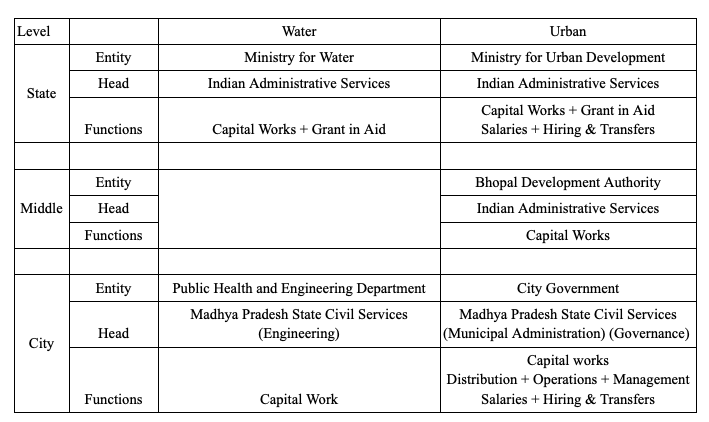
\includegraphics[width=1\textwidth]{images/Bwater.png} % Adjust the width as needed
    \caption{Bhopal's Administrative Water Delivery Chart. Source: Different Sources}
   
\end{figure}


Bhopal's successful water governance largely stemmed from its effective use of state-level bureaucrats recruited through the Madhya Pradesh State Civil Services (Provincial Services). These officers, primarily from Municipal and General Administration cadres, served in crucial positions like Assistant and Additional Commissioners, bridging the gap between elite Indian Administrative Service (IAS) officers and frontline staff. Unlike their IAS counterparts who viewed urban postings as temporary career steps, Provincial Service officers maintained longer tenures in city assignments.In this respect, these state-level bureaucrats closely resemble their counterparts in Lucknow, where similarly recruited officers oversee both the city’s water utility (the Lucknow Jal Sansthan) and its municipal administration (the Lucknow Municipal Corporation). This continuity enabled these bureaucrats to develop deep local expertise and institutional memory while working within established administrative frameworks, ultimately contributing to more effective urban governance. As one state bureaucrat explained succinctly:
\begin{quote} “We are here for the rest of our lives. This is our work, and if we do not do this, who will?”\footnote{Interview with an officer of the Madhya Pradesh State Civil Services (Municipal Administrative Services Cadre). Bhopal 2022)
} \end{quote}

This embedded position allowed these officers to navigate the vertical hierarchies of elite IAS officials above them and the horizontal complexities of city departments and frontline staff below. Far from achieving full autonomy, they still had to accommodate legitimate political pressures and community demands. Yet their relative permanence and localized knowledge created a form of partial insulation—the crux of conditional autonomy—allowing them to maintain technical standards, initiate reforms, and adapt strategies over time.

The institutional framework enabling such bureaucratic intermediation took concrete shape through substantial development funding: \$346 million drawn from an Asian Development Bank (ADB), JnNURM and Department for International Development (DFID) which lasted from 2006-2014.\footnote{These funds were channeled through the Madhya Pradesh Urban Services for the Poor (MPUSP) and Madhya Pradesh Urban Water Supply and Environmental Improvement in Madhya Pradesh Project (MPUSEI) initiative, which included two flagship programs: UDAY (a loan by ADB) focused on strengthening physical infrastructure, and UTHAN (untied grant by DFID) targeted institutional reforms, better revenue management, and enhanced administrative practices. This flow was supported by JnNURM a reform contingent grant from the Union Government.} This infusion of capital did not simply erect infrastructure; it also reshaped bureaucratic practices.  Unlike Lucknow—where project units operated at a remove from municipal structures—Bhopal integrated its Project Implementation Unit (PIU) directly into the Bhopal Municipal Corporation (BMC).\footnote{Interview with the City Team Leader from DFID (2006-2009) Zoom 2021 2022.} International agencies also did more than supply funds: they adapted their oversight mechanisms to work within, rather than bypass, state structures, creating a rare synthesis between international development expertise and local institutional realities. 

The PIU assembled about 30 full-time professionals, including both consultants and state bureaucrats, all required to maintain a constant presence in Bhopal.\footnote{See annexure for the organizational design of PMU, PIU} The consultants’ technical expertise, external affiliations, and alignment with global governance norms enhanced the PIU’s standing. Their sustained involvement and proximity conferred a form of prestige and recognition often associated with external validation—what some scholars characterize as “symbolic capital” \citep{bourdieu_forms_1986}. Meanwhile, state bureaucrats, with long-term commitments to regional administration, contributed local knowledge and institutional memory. Although senior leadership (consultant team leaders and elite IAS project heads) frequently rotated, a core group of consultants and state officials remained, fostering stable relationships, shared norms, and collaborative problem-solving that bridged external expertise and local realities.\footnote{A project manager at the state level, typically an IAS officer, was appointed specifically to work with this group for a two-year term.}

Three key developments illustrate how this incremental capacity-building advanced the city’s governance norms. First, the Project Implementation Unit (PIU) deliberately diversified skill sets beyond engineering, incorporating procurement specialists, public finance professionals, and urban governance experts.\footnote{Interview with the officers of the Madhya Pradesh State Civil Services who were part of the PIU. Bhopal 2021 2022 2023} This broadened perspective reframed urban challenges—from water delivery to waste management—not as siloed engineering problems but as multifaceted governance issues involving human resources, coordination, and institutional design. By embedding these varied competencies, the PIU internalized new problem-solving approaches and routine practices. 

Second, capacity-building targeted systemic weaknesses in human resource management. City-level hiring had traditionally been influenced by patronage, leaving technical roles in engineering, sanitation, auditing, and public health under-skilled and unevenly staffed. Recognizing that these issues were not unique to Bhopal but endemic across Madhya Pradesh’s urban sector, state-level bureaucrats leveraged their embedded position to initiate institutional reforms.\footnote{Interview with Devinder Chauhan, Madhya Pradesh State Administrative Services, Bhopal, 2022. This version was corroborated by Bruce Pollock and Jim Arthur, both of whom were DFID officers in Madhya Pradesh. Zoom 2022, 2023.
} One officer complained that District Magistrate (DM)-oriented IAS training “didn’t prepare them for cities":

\begin{quote}
    “Other cities [like Gwalior, Indore, Jabalpur, and Ujjain] faced similar issues. We raised these staffing concerns with the Commissioner, but they didn’t prioritize them. Urban is a very small part of a District; officers mostly deal with schemes for rural areas. Their field training as District Magistrates (DMs) didn’t prepare them for cities.  \textit{Woh municipal ko samjah hi nahin sakte} (They cannot understand cities).”\footnote{Interview with an officer of the Madhya Pradesh State Civil Services (Municipal Administrative Services Cadre).
Bhopal 2022}
\end{quote}

Another added 

 \begin{quote}
“These engineers, tax inspectors would be our problem in the long term. We have to face them [for the entire duration of their career], not those in the \textit{Sachivalaya} (Secretariat).”\footnote{Interview with an officer of the Madhya Pradesh State Civil Services (Municipal Administrative Services Cadre).
Bhopal 2022}

 \end{quote}

 These reflections underscore a power dynamic and professional identity distinct from the IAS-dominated paradigm. The state cadre officers, more deeply embedded in urban contexts, leveraged their position to introduce reforms that aligned long-term city interests with institutional capabilities. By pushing beyond conventional hiring patterns, these officers created conditions where stable, competency-driven staffing could emerge as the norm. Collaborative exercises motivated by these state bureaucrats culminated in the creation of a Standard Departmental Structure, comprising 10 departments and 110 designations, alongside the establishment of five new municipal cadres—Accounts, Revenue, Engineering, Sanitation, and Executive services—and a revision of Service Rules to institutionalize these changes.\footnote{Oxford Policy Management. (2012). \textit{Project completion review: Madhya Pradesh Urban Services for the Poor (MPUSP) Project}. Available at: \nolinkurl{https://iati.fcdo.gov.uk/iati_documents/3780261.odt}} This internal cadre reform geared towards the cities, was not simply a technical adjustment; it represented the codification of new norms into formal structures. An independent end of project evaluation  acknowledged: “[It] appreciates the above interventions that had to overcome considerable on-ground challenges.”\footnote{ibid., page 9}

A third issue—how to sustainably ramp up capacities over time—centered on core public management tasks. In the 2000s, BMC faced challenges common to Indian cities: procurement, tender preparation, quality control, and complex Management Information Systems (MIS) implementation. The DFID grant provided specialists in administration, e-governance, communications, finance, engineering, social development, GIS, and energy.\footnote {Proposal for Financial Assistance Under Madhya Pradesh Urban Services for the Poor (MPUSP) Programme, Department for International Development (DFID), January 2007, Bhopal.}
However, the impetus for these changes did not come solely from elite IAS officers; the groundwork was laid by the state bureaucrats who engaged directly with frontline bureaucrats—tax assessors, computer operators, engineers, and others—to institutionalize these changes. Over time, state cadre officers developed technical expertise in tendering, procurement, and advanced tools like GIS and MIS. Large-scale training initiatives—12,000 city government staff trained across six cities, including Bhopal—further strengthened these emerging competencies.\footnote{Oxford Policy Management. (2012). \textit{Project completion review: Madhya Pradesh Urban Services for the Poor (MPUSP) Project}. Available at: \nolinkurl{https://iati.fcdo.gov.uk/iati_documents/3780261.odt}} From a theoretical standpoint, these capacity-building efforts represent a form of social learning and collective adaptation. As bureaucrats gained new skills and witnessed the benefits of improved procedures, these practices became internalized as standard operating procedures. This gradual normalization of improved management and technology adoption created norms which spread via professional networks, path dependence, and the pursuit of organizational legitimacy.

The property tax reforms exemplify how these reforms produced tangible, if partial, results. As in Lucknow, external financing conditions required municipal revenue improvements. However, raising water tariffs proved politically contentious, as political resistance at the city and state levels , similar to Lucknow stymied any moves toward metering or pricing increases.\citep{sen_issues_2022} A DFID team leader observed:

\begin{quote}
    "This was not just Bhopal. Getting politicians in India to increase tariffs is a problem. We tried to convince the bureaucrats, actually—that, I think, was the key to our work. Our strategy was to talk to the bureaucrats, and they would then talk to the politicians."\footnote{Interview with Dr Bruce Pollock, Project Manager Kathandu Nepal 2022 Zoom 2024}
\end{quote}

DFID was encouraged by the state cadre officers to focus on expanding the property tax base instead of pushing politically sensitive water tariff hikes. With only 46\% of properties taxed, this represented a substantial revenue opportunity.\footnote{\textit{Budget document, Lucknow Municipal Corporation}, 2005–2014.} The state officers in their field experience as well as inputs from the revenue officers noted that the base was low and if increased to 90\% of properties - a move that would substantially increase municipal revenue without requiring politically sensitive rate hikes. This approach sidestepped direct political opposition to metering or price increases, aligning bureaucratic goals with political interests more smoothly.  

Below is a revised version that aims for greater clarity and coherence:

The expansion of Bhopal's property tax base was guided by a systematic, state bureaucrat–led strategy. Officers were first trained in property evaluation techniques and began by surveying newer areas before moving on to established neighborhoods. This phased approach was bolstered by technical innovations such as GIS mapping and automated tax calculation tools, which together produced an integrated property database linked to cadastral records and revenue maps \citep{awasthi_property_2020}. A key milestone in this process was the introduction of a centralized Management Information System (MIS)—making Bhopal the second Indian city, after Mumbai, to implement one.\footnote{The implementation of the MIS is discussed in detail in the chapter on Trash.}

To support these changes, state bureaucrats navigated political resistance to digital modernization and expanded on-the-ground capacity by increasing the number of tax assessors from 22 to 148. They institutionalized regular monitoring through monthly meetings on door-to-door surveys and introduced unique household property IDs.\footnote{Oxford Policy Management. (2012). Project completion review: Madhya Pradesh Urban Services for the Poor (MPUSP) Project. Available at: \url{https://iati.fcdo.gov.uk/iati_documents/3780261.odt}} Attention to both technical and administrative details underpinned the reform’s success. State bureaucrats regularly updated tax registers, established grievance redressal mechanisms within municipal offices, and managed political demands for tax amnesties and exemptions. In doing so, they maintained the integrity of the system while accommodating legitimate concerns.


In Bhopal, while property tax reforms significantly bolstered revenue administration—with collections rising from \$3.73 million in 2006–07 to \$9 million in 2011–12—dependence on state and union grants persisted.\footnote{Proposal for Financial Assistance Under Madhya Pradesh Urban Services for the Poor (MPUSP) Programme, Department for International Development (DFID), January 2007, Bhopal.} Meanwhile, revenue from water remained negligible, as only 3\% of households had meters in 2022, indicating the political reluctance to tackle more contentious reforms like raising water tariffs. This partial success illustrates a familiar dynamic: technical and administrative reforms can tackle immediate, manageable issues but rarely overcome entrenched political and structural barriers. From a theoretical standpoint, this outcome aligns with the notion that state-level bureaucrats often succeed with “low-hanging” administrative fixes—such as broadening the property tax base—but struggle to secure political support for more challenging measures. The reluctance to confront the politically sensitive issue of water charges underscores how technical progress can coexist with underlying governance dilemmas. Yet, by focusing on what was politically feasible—enhancing skill sets, standardizing departments, and improving procurement and MIS systems—state cadre officers and their allies created a more resilient administrative environment. Although these adjustments did not fundamentally alter the political economy of urban service delivery, they established a crucial foundation for addressing more complex issues of political-business relations and community engagement, topics explored in the following sections. In this sense, the Bhopal case illustrates that bureaucratic intermediation, while not transformative in itself, can still produce meaningful gains amid persistent political constraints.


\subsection{Managing Political-Business Relations: The Art of Bureaucratic Intermediation}

The previous section outlined how Bhopal’s state-level bureaucrats gradually built institutional capacity and internalized new governance norms, reinforcing the partial insulation central to conditional autonomy. Another, more intricate challenge emerged as significant development funding—approximately \$346 million from various agencies—flowed into the city. Now, beyond just ensuring technical proficiency and incremental reforms, bureaucrats had to manage the political economy of large-scale infrastructure projects. This elevated the stakes considerably: politicians viewed these funds as potential patronage opportunities, and local contractors—despite their experience in small-scale work—struggled with advanced technical standards demanded by international funders. As these massive projects got underway, rather than operating under full insulation or succumbing to pure instrumentalization, these officials found themselves navigating a contested space where political pressures and market forces converged. They needed to uphold minimum quality standards and maintain project coherence, even as political actors pushed for favoritism and contractors lobbied for easier conditions. Merely applying formal procurement guidelines or technical manuals was insufficient. The situation called for informal negotiation, persuasion, and adaptive strategies.

The unprecedented scale of development funding created new political–business dynamics.  Local contractors, skilled at small-scale municipal works, suddenly faced FIDIC-based contracts \footnote{FIDIC (Fédération Internationale Des Ingénieurs-Conseils) contracts are standardized construction contracts developed by the International Federation of Consulting Engineers. These contracts set global standards for complex infrastructure projects, including detailed specifications for risk allocation, quality control, and dispute resolution. While standard in international development projects, they marked a significant departure from traditional municipal contracting practices in Indian cities.}, stringent quality thresholds, and global best practices. This mismatch created instability: opaque procurement rules, lowest-bidder selection criteria, and a dearth of familiarity with ADB procedures produced confusion and risk premiums.\footnote{Proceedings from the MP Urban (ADB) Project at the R.C.V.P. Noronha Academy of Administration and Management Bhopal on "Procurement under MP Urban (ADB) Project".} Existing arrangements—where internal settlements and “lowest bidder wins” often led to substandard work.\footnote{Interview with Dr Bruce Pollock, Project Manager (2006-2009) Kathandu Nepal 2022 Zoom 2024} Without actors capable of bridging information gaps, interpreting technical requirements, and mediating disputes, implementation would have stalled.

Here, state bureaucrats emerged as essential mediators. While consultants ensured formal compliance, they alone could not unravel the complex interplay of political patronage, contractor ambitions, and administrative constraints. Politicians, anticipating new patronage channels, pressured to direct contracts to favored firms. Some contractors with checkered pasts but strong political links sought re-entry into bidding.\footnote{Chouhan, S. S. (n.d.). Transforming Madhya Pradesh. Skoch Group. Retrieved from https://books.skoch.in/shop/books/transforming-madhya-pradesh-shivraj-singh-chouhan/} Elite IAS officers, steeped in formal roles and wary of compromising professional neutrality, hesitated to intervene directly. State-level officers, by contrast, leveraged their unique position—characterized by long-term urban postings and deep local networks—to bridge these divides. They recognized that formal procurement rates often failed to reflect market realities, creating perverse incentives for corruption and compromised quality. Their response was multi-tiered: public consultative meetings addressed formal bidding processes,\footnote{Meeting records show that contractors themselves raised concerns about corruption among city engineers. Politicians, meanwhile, pointed to bureaucratic intransigence and favoritism - a circular blame game ensued. } while smaller "vision alignment" sessions provided space for stakeholders to air grievances and negotiate workable solutions. Through these iterative negotiations, state bureaucrats developed practical innovations. They restructured large projects into smaller "packages" accessible to local contractors while maintaining quality standards. They worked with consultants to clarify technical requirements and adjusted tender specifications to reflect realistic costs. This approach did not eliminate informal practices but channeled them into more transparent, manageable arrangements. The result was a pragmatic framework that balanced political imperatives with administrative necessities.

Bhopal’s then-Mayor, Sunil Sood, candidly encapsulated these political realities.

\begin{quote}
``\textit{Thekedar} (Contractors) are a vital part of the process and an essential component of the world we work in. I am in power now, tomorrow I am in the opposition. If I will not accommodate their interests [contractors linked with opposition city leaders], why will they accommodate mine?"\footnote{Interview with Sunil Sood, Congress led Mayor of Bhopal City Government (2004-2009), Leader of Oppostion (2009-2012) Leader of Bhopal City Council (2000-2004), City Councillor (1995-2009). Bhopal 2021, 2022, 2023) 
}
\end{quote}

This statement underscores the political realities that formal institutional designs rarely capture. Similarly, the then Project Director from the elite IAS 
 cadre, Manish Singh, acknowledged the complexity:

\begin{quote}
``You can understand the implications of getting these contractors in the office. Negotiating is not my job, its the politicians. But  we as bureaucrats also have to get involved... I did ask my deputies to look into this—they knew the landscape better."\footnote{Interview with Manish Singh, Project Director - Madhya Pradesh Urban Services Improvement Program}
\end{quote}

These comments reveal a crucial distinction: while elite IAS administrators maintained formal distance, state bureaucrats engaged directly in day-to-day negotiations. Their long-term presence in the system provided them with institutional memory and deep local networks. Acting as boundary spanners \citep{tushman_boundary_1981}, they bridged the gap between politicians, contractors, and consultants. Unlike IAS officers constrained by formal rules and expectations of political neutrality, these state bureaucrats could work through informal channels, leveraging their relationships to secure resources and build consensus among stakeholders.



\begin{table}[ht]
\centering
\begin{tabular}{l l l l}
\toprule
\textbf{State} & \textbf{Capital Works} & \textbf{Operations \& Management} & \textbf{Revenue Functions} \\
\midrule
Madhya Pradesh    & State \& City Government        & City Government                   & City Government \\
Uttar Pradesh     & State \& City Government        & Parastatal \& City Government     & Parastatal \& City Government \\
Andhra Pradesh    & State                           & City Government                   & City Government \\
Bihar             & State                           & State                             & City Government \\
Chhattisgarh      & State                           & State                             & City Government \\
Gujarat           & State \& City Government        & City Government                   & City Government \\
Himachal Pradesh  & State                           & State                             & City Government \\
Karnataka         & State \& City Government        & City Government                   & City Government \\
Kerala            & State                           & State                             & State \\
Maharashtra       & State \& City Government        & City Government                   & City Government \\
Orissa            & State                           & State                             & State \\
Rajasthan         & State                           & State                             & State \\
\bottomrule
\end{tabular}
\caption{Overview of responsibilities in various Indian states.}
\label{tab:state-functions}
\end{table}





A pivotal episode narrated by the Mayor captures this delicate equilibrium. When contractors claimed rising material costs made current rates untenable, the Mayor convened a meeting of all stakeholders—engineering staff from the Public Health and Engineering Department (PHED), contractors, councilors—and tasked a state bureaucrat leading the Bhopal PIU and his team to mediate. As the Mayor recalled:

\begin{quote}
    “During my tenure, all this JnNUURM money came in. Work continued for eight years and the prices of pipes and earthwork rose, prompting the contractors to say they couldn’t continue at the current rates. Naturally, we couldn’t just approve higher rates without proper scrutiny. So I asked Mayan [State bureaucrat and Urban Governance Officer in the PIU] to bring his team. Everyone involved—engineering staff and contractors, councilors —and had them sit down together. I told them, ‘Look, we’re willing to consider what’s reasonable, but you can’t simply top-up on another 5-6\%. Then I asked directly, ‘How much commission is being paid here?’
The room went silent. I pointed out that the people who pay commissions and those who receive them are in the room, so there was no point hiding it. Eventually, they [contractors] admitted that the commission [to engineers of the PHED] of the amounted to around 12-14\%. I said, ‘Cut it down. If you’re giving 12\%, bring it down to about 5\%.  Mayank asked the chief engineer if this was an acceptable arrangement. He [Mayank] told them when there were no big projects, nobody made much. This is a 500 crores (about \$100 million) project, if this is delivered, more will come.’”\footnote{Interview with Sunil Sood, Congress led Mayor of Bhopal City Government (2004-2009), Leader of Oppostion (2009-2012) Leader of Bhopal City Council (2000-2004), City Councillor (1995-2009). Bhopal 2021, 2022, 2023) 
}
\end{quote}

These interactions were themselves a form of political signaling, where contractors and politicians used the meeting as a platform to communicate their demands and expectations. When quizzed about this corruption in general and this particular meeting in particular, the bureaucrat suggested how the contractors had to be involved in the way that the politicians wished: 

\begin{quote}
    “There are two kinds of pressure that politicians put on us: one is positive pressure, where public work needs to be done and they protest if it doesn’t happen accordingly. The other is negative pressure, where politicians pressure us to give their people contracts or withhold contractors’ payments. These meetings are part of that negative pressure—the contractors and politicians talk, and they want us to know what they want. You have to work in this framework, otherwise nothing would have happened.” \footnote{Interview with Mayank, Madhya Pradesh Administrative Services (Governance Cadre) Urban Governance Officer PIU Bhopal 2022
}
\end{quote}

Such negotiations reflect not a moral endorsement of corruption but a strategic containment approach consistent with the logic of conditional autonomy. Rather than an idealized “co-production” process free from rent-seeking, what occurred was a negotiated settlement where everyone aligned on a “doable” compromise. The state-level bureaucrats accepted certain informal practices as given, yet shaped them to protect minimum quality and efficiency standards. They leveraged their informal networks and standing as long-term urban administrators to reduce exaggerated commissions, insist on minimal technical thresholds, and subdivide contracts to lower barriers for local contractors. This recalibration prevented project collapse and ensured forward momentum—“getting things done” amid complexity and entrenched interests.

\vspace{12mm}

Consultant involved on the behalf of DFID elaborated:

\begin{quote}``We know there would be corruption, but what we cared about was the end outcome... These bureaucrats faced similar challenges in other cities as well, so we provided them with broad contours of the project, but they had to do the coordination and we tried our best to accommodate.”\footnote{Interview with Richard Slater, Governance Advisor 2009-2012 PIU. Tripline Consultancies} \end{quote}

This statement emphasizes that state-level bureaucrats were not merely implementing predetermined policies; they were actively shaping the project’s trajectory through negotiated intermediation. This instance exemplifies conditional autonomy in moments when elite IAS officers granted minor freedoms. Although not fully insulated from political pressures nor entirely captured by them, these bureaucrats adapted and leveraged informal norms—such as the “vision meetings” mentioned here—to achieve workable compromises. This scenario aligns with theories suggesting that in low-capacity environments, certain informal arrangements, while normatively undesirable, can serve as “lubricants” facilitating the execution of large-scale infrastructure projects.


Bhopal’s experience thus reveals that “getting things done” in complex institutional contexts often involves balancing political demands, contractor interests, and technical standards. State-level bureaucrats, with their dual role as “intermediaries within and outside the state,” managed to navigate these conflicting objectives without completely surrendering to either political patronage or technocratic rigidity. In effect, the state bureaucrats’ approach deviates from idealized governance models but still advances some developmental goals. By containing and structuring informality—reducing exaggerated commissions, insisting on minimal quality thresholds, subdividing contracts to lower barriers to entry—they constructed a more manageable political-business environment. These partial controls and incremental adjustments reinforced a set of emerging norms and practices consistent with conditional autonomy. Thus, rather than weakening the case for institutional reform, these actions underscore the complexity of governance challenges and the nuanced role that officials play in forging workable solutions under less-than-ideal conditions.

Having illustrated how state bureaucrats moderated political-business relations, I now move to the final dimension of Bhopal’s conditional autonomy: legitimizing community participation and addressing the persistent gap between infrastructure creation and sustainable, equitable service delivery

\subsection{Beyond Infrastructure: The Limits of Conditional Autonomy in Service Delivery}

Having seen how state-level bureaucrats in Bhopal moderated political-business relations to push large-scale projects forward, I now consider another aspect: ensuring that the expansions in infrastructure translate into sustainable, equitable service delivery. Thus far, I have identified these state officers as pivotal intermediaries—operating both within and outside the state—to accommodate political pressures and market imperatives without collapsing into pure patronage or rigid technocracy. Yet, their engagement with slum communities reveals both the promise and the limitations of this approach. While bureaucratic intermediation improved access and legitimacy, it struggled to deliver consistently high-quality services, illustrating what the I call “precarious universalism.”

Delivering water to Bhopal’s slums laid bare the complexity of local political and bureaucratic economies. Politicians, who wielded influence over pipeline extensions, tanker allocations, and borewell installations, often used these resources selectively, reinforcing patterns of patronage.\citep{auerbach_neighborhood_2017} In some instances, certain marginalized groups—migrants, religious minorities, Dalits, and Tribals—found themselves systematically deprioritized. Meanwhile, frontline engineering staff and field-level workers extracted petty rents by controlling pump schedules or influencing maintenance decisions.  Although DFID’s grant required prioritizing slums in public goods delivery, my interviews and field observations suggest that the complexity of local political economies and bureaucratic hierarchies demanded more than a top-down reform agenda.  Instead, state-level bureaucrats had to step in as credible intermediaries who could legitimate community-driven solutions while maintaining at least minimal adherence to technical and administrative standards.

DFID’s emphasis on slum improvement offered an opening to challenge these patterns. With Bhopal ranking 13th among India’s 132 cities in terms of slum population, the scale of the task was immense. Baseline surveys reported only 30\% piped water coverage in slums, with most residents traveling significant distances for basic needs. In principle, DFID’s protocols called for partnering with Non Governmental Organizations (NGOs) to foster community participation (Figure 1.7).\citep{kutter_demystifying_2014} Yet as one Mayor derisively put it,—``Woh toh paisa banne wale log hai. Na idhar ki baat karte hai no udhar ki" (“They’re just there to make money; they neither speak for here nor there”) \footnote{Interview with Krishna Gaur, Mayor of Bhopal (2009-2014), Bhopal 2021, 2023}— civil society organizations  lacked both entrenched urban poverty expertise and the political trust necessary to challenge established bureaucratic and political interests. Building legitimacy and meaningful engagement required a different catalyst.

\begin{figure}[H] % Use [H] to force the image to appear exactly where you place it
    \centering
    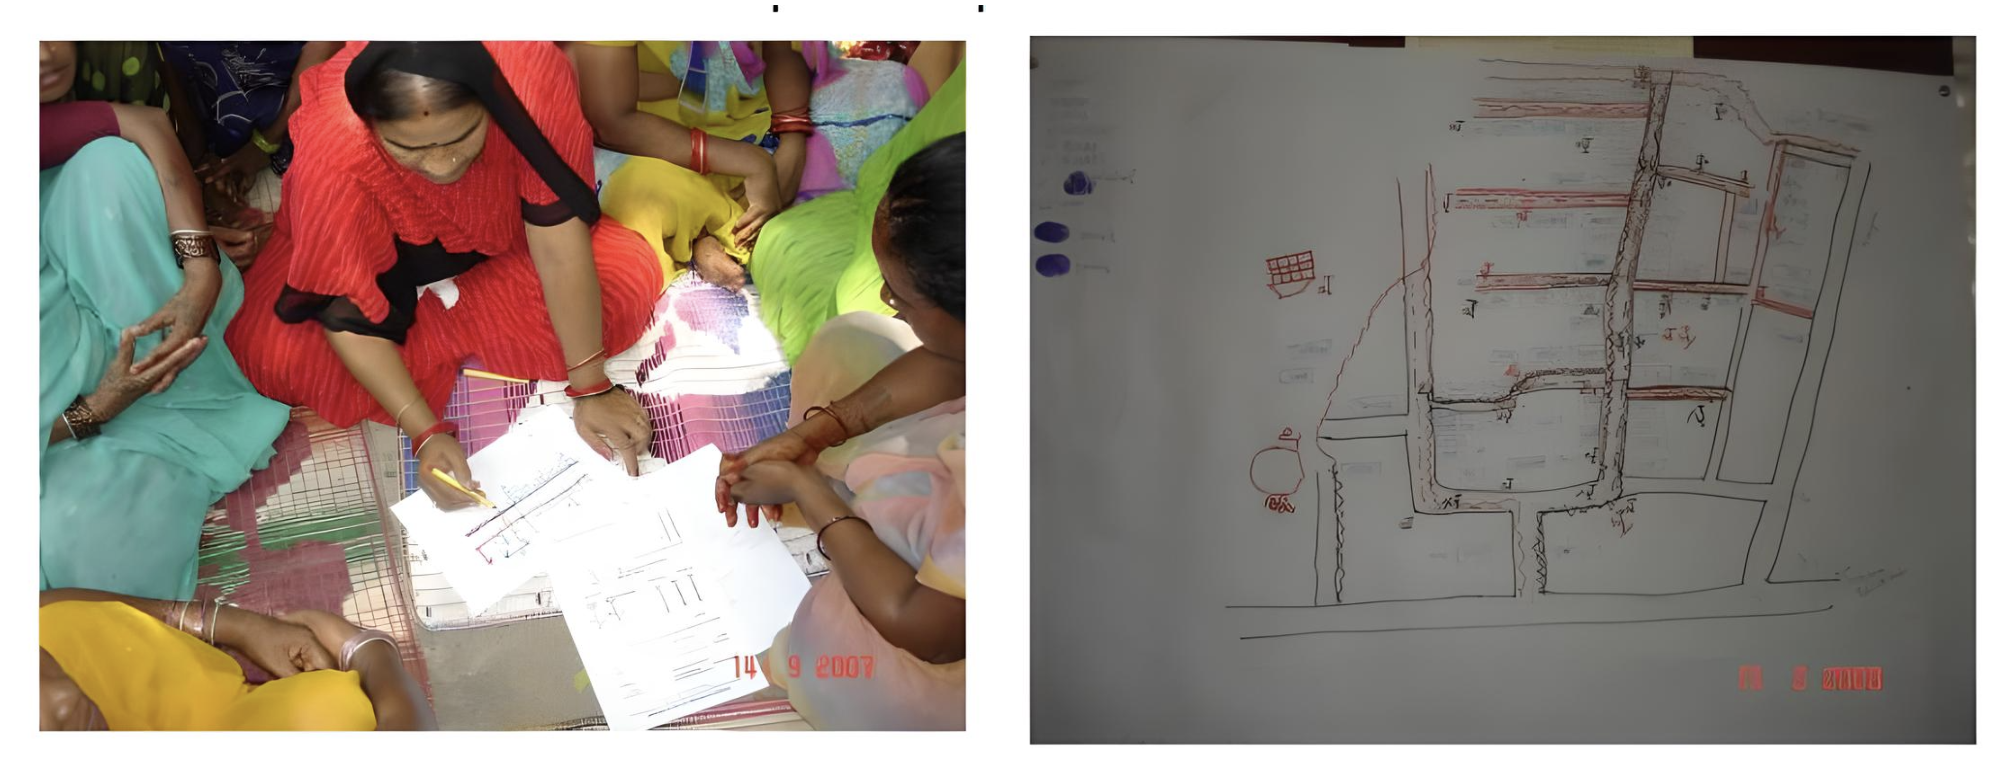
\includegraphics[width=1\textwidth]{images/Screenshot 2024-12-14 at 17.16.40.png} % Adjust the width as needed
    \caption{Left: Slum Management Committees working with civil society members under the DFID project. Right: Neighborhood Map for audit. Source: Provided by NGO SAMARTHAN. Bhopal 2022}
   
\end{figure}



Here again, state-level bureaucrats performed a critical bridging function. They worked with NGOs—sometimes reluctant partners—and formed community committees to oversee contractor performance.\citep{kumar_barriers_2016} Crucially, DFID’s requirement for public hearings before releasing payments to contractors granted these committees a formal oversight tool. While frontline staff and contractors might collude to justify incomplete work, committees armed with official sanction and supported by recognized bureaucrats could push back. As one NGO representative noted:
\begin{quote} “When these state bureaucrats would come visit, they also made sure other department officers came—water works, urban development, revenue, and municipal corporations. Our presence was legitimized if the officer was there; otherwise, we were not that important.”\footnote{Interview with members of AARAMB, Bhopal based civil sociey organization. Bhopal 2022, Zoom 2024} \end{quote}


Pushed by DFID on the top and the civil society organization in the bottom, state-level bureaucrats lent their institutional authority—and their embedded networks in the city administration—to turn community committees from nominal watchdogs into actors with real leverage. They thus moved beyond mere facilitation to active legitimization of community-driven solutions. In slums like Bagmugaliya,\footnote{established in 1983Despite having 148 households and a population of 740, this slum had no regular water source and relied entirely on tanker supply. }  residents pooled resources to create localized piped networks or install pumps, despite such measures being technically “illegal” or at least noncompliant with municipal regulations.\citep{noauthor_poverty_2006} Similar grassroots solutions emerged elsewhere—one community financed a pump to serve uphill residences; another built a common septic tank. Municipal guidelines deemed such arrangements improper due to issues like inadequate pipe depth or lack of structural integrity. Post-2014 regulatory shifts learned and even allowed some previously informal solutions to be integrated into municipal systems.


By reframing these improvised infrastructures as necessary stopgaps toward last-mile connectivity, bureaucrats convinced frontline staff and even some IAS superiors to tolerate these arrangements. Involving elected officials ensured political cover, while consulting technical experts and setting minimal performance standards prevented egregious risks. This delicate balancing act exemplifies conditional autonomy in action: bureaucrats operating in a gray zone, between strict enforcement of regulations and total political acquiescence, crafting pragmatic compromises that advanced coverage—if not impeccable compliance.\footnote{ As one civil society organization observed, "the authorization for the same has to come from the elected officials... and through negotiations with the frontline and upper-tier bureaucrats." The bureaucrats' ability to convert potentially contentious informal arrangements into accepted practice, while maintaining program objectives and getting street-level bureaucrats and politicians on board, was crucial for success.}
 

Yet these accomplishments came with clear constraints. While pipes and pumps proliferated, consistent water pressure and reliability lagged behind. Field research and citizen surveys revealed a stark contrast: although near-universal access (93\% in shacks, 97\% in slums) was achieved, about 70\% of shack residents and 36\% of slum households received water for only one hour per day (Table 1.6 and Figure 1.8). This illustrates “precarious universalism”: a condition where coverage becomes widespread, but remains unstable and uneven. The system could easily revert to earlier dysfunction once external oversight or donor involvement subsided.


\begin{table}[ht]
\centering
\renewcommand{\arraystretch}{1.3} % Adjust row height
\setlength{\tabcolsep}{5pt} % Adjust column spacing
\begin{tabular}{|p{3cm}|p{3cm}|p{3cm}|p{3cm}|p{3cm}|}
\hline
\textbf{City} & \textbf{Housing Type} & \textbf{Tap (Piped)} (\%) & \textbf{Borewell + Hand Pump} (\%) & \textbf{Other Sources} (\%) \\ \hline
Bhopal & Shack & 93 & 1 & 6 \\ \cline{2-5}
       & Slum  & 97 & 2 & 1 \\ \hline
Lucknow & Shack & 48 & 37 & 15 \\ \cline{2-5}
        & Slum  & 64 & 32 & 4 \\ \hline
\multicolumn{5}{l}{\textit{Source: Primary survey under the Brown - India Citizenship Project 2022}} \\ % Add source note
\end{tabular}

\caption{Source of Water by City and Housing Type (Shack and Slum Only)}
\label{tab:water_shack_slum}
\end{table}



\begin{figure}[H] % Use [H] to force the image to appear exactly where you place it
    \centering
    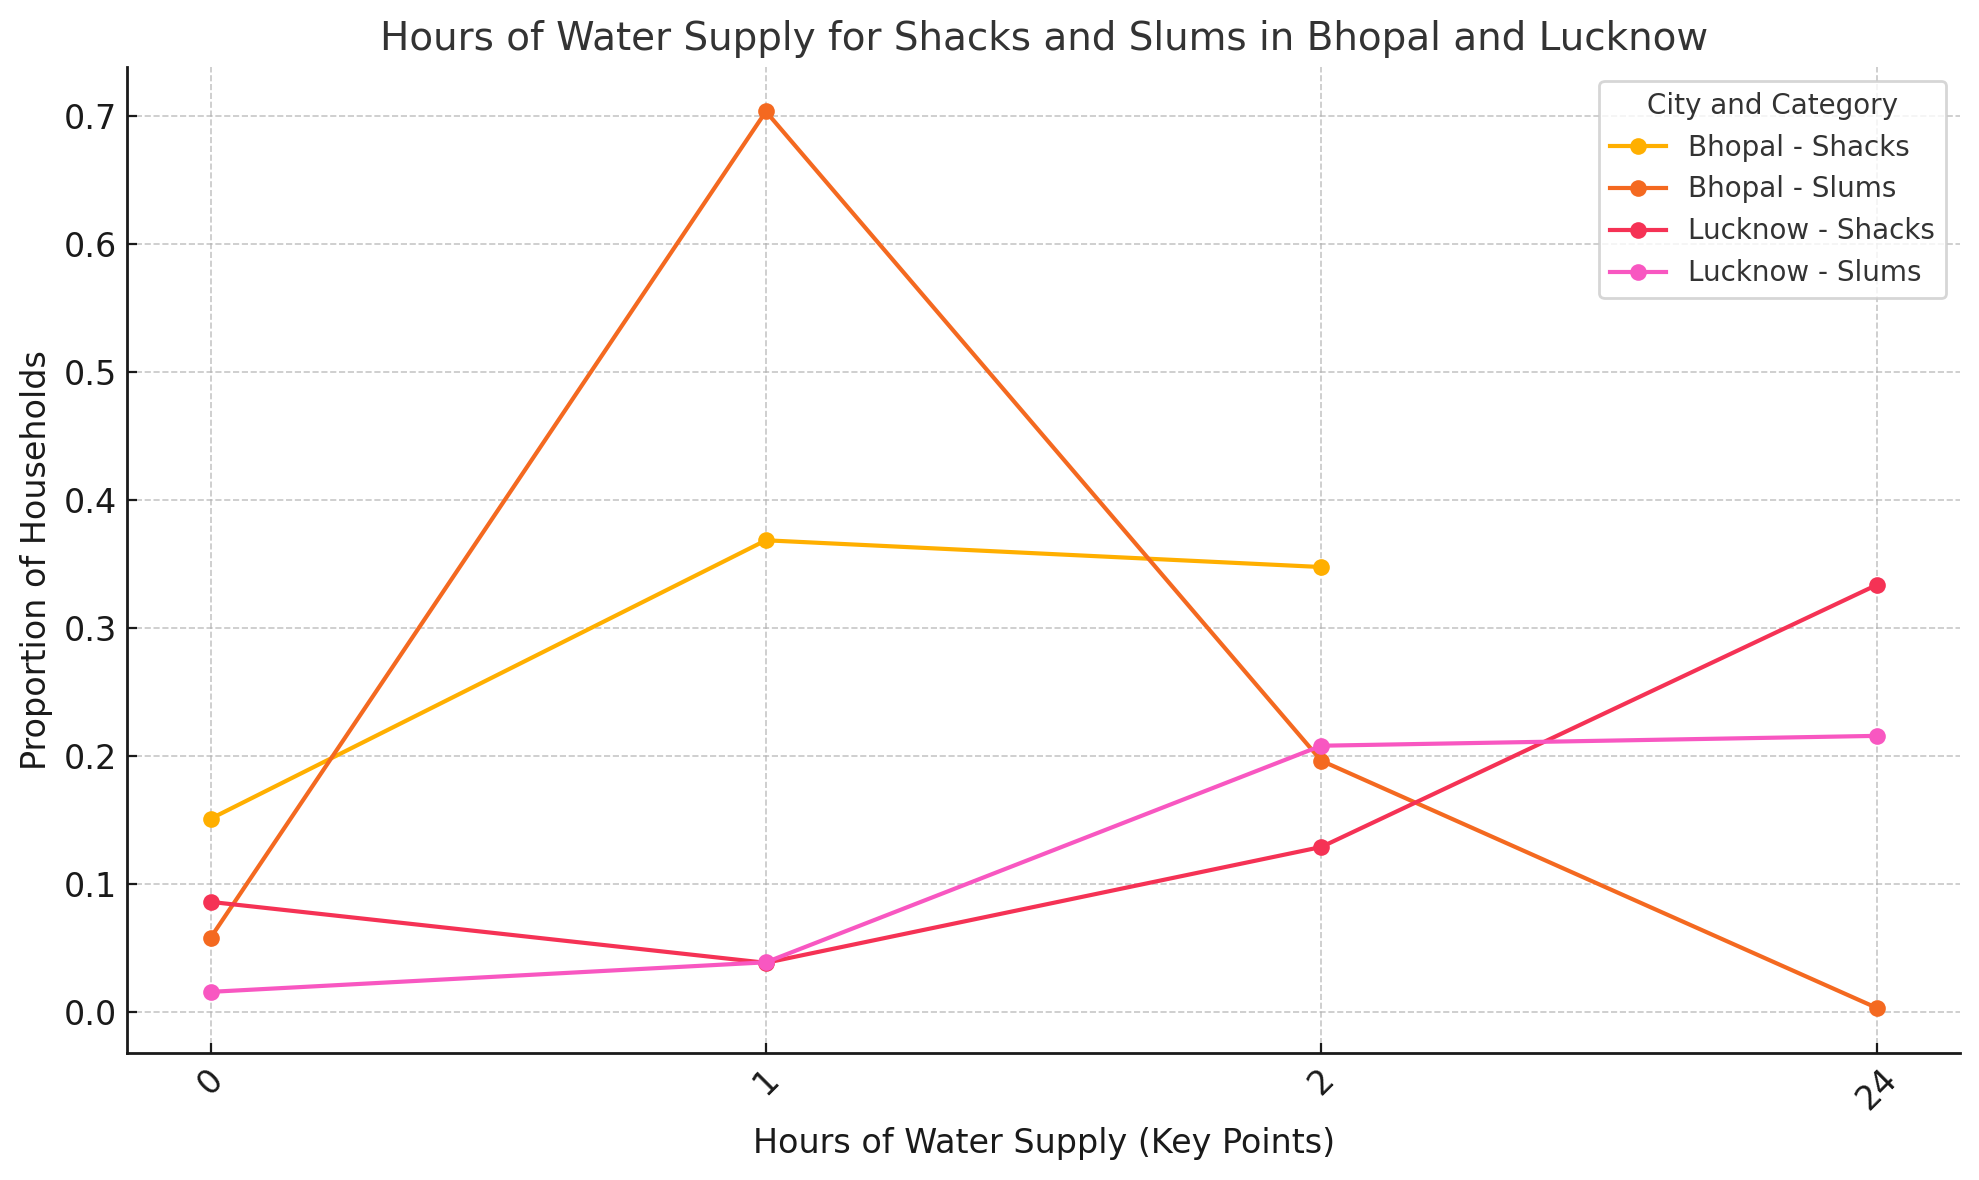
\includegraphics[width=1\textwidth]{images/water comparison-slum and shack.png} % Adjust the width as needed
    \caption{Hours of water suppply in the informal housing (slums and shacks) of Bhopal and Lucknow. Source: Primary survey under the Brown - India Citizenship Project 2022}
   
\end{figure}



While state-level bureaucrats could harness their unique position to overcome immediate implementation hurdles—navigating political pressures, adapting to local norms, and legitimizing community-driven solutions—they could not, on their own, sustain long-term improvements in service quality. Two main factors contributed to this constraint. First, bureaucratic incentives and donor metrics focused heavily on visible, quantifiable achievements—such as the number of new connections—rather than on long-term reliability or daily supply hours. Once external monitoring waned, maintenance and pressure management slipped, revealing the fragility of gains secured through negotiated compromises. Second, DFID’s intervention, though crucial in spurring community committees and slum focus, did not fundamentally alter the deeper political and institutional matrices governing service delivery. Entrenched patronage networks and frontline rent-seeking practices persisted. Without deeper transformations—empowering civil society beyond donor timelines, strengthening accountability mechanisms, and realigning political incentives—conditional autonomy could not evolve into a more genuinely programmatic or stable arrangement.

Bhopal’s experience in slum service delivery thus underscores both the strengths and inherent limits of bureaucratic intermediation under conditional autonomy. State-level bureaucrats could deftly navigate political-business conflicts, legitimize community participation, and secure widespread access, demonstrating the approach’s capacity for positive incremental change. Yet the enduring gap between infrastructural coverage and actual service quality, and the ease with which improvements could erode in the absence of sustained oversight, highlight that conditional autonomy is no panacea. Rather, it is a fragile equilibrium that can facilitate immediate progress but may struggle to deliver lasting institutional transformation.

In conclusion, while bureaucratic intermediation proved effective in surmounting immediate obstacles and achieving more inclusive coverage, ensuring consistent, high-quality service demands systemic changes that surpass the limited scope of these negotiated arrangements. Absent robust, long-term accountability structures, strong civil society engagement, and the reorientation of political incentives to value sustainability over short-term gains, precarious universalism will likely persist. Bhopal’s case, therefore, reinforces the idea that conditional autonomy—essential for navigating complexity and partial reform—is ultimately a stepping stone, not the final destination, in the pursuit of equitable and durable urban governance.

\subsubsection{Conclusion}
Bhopal’s trajectory illustrates that even in a context shaped by patronage politics, infrastructural complexity, and uneven bureaucratic capacity, state-level bureaucrats can forge a degree of conditional autonomy that yields meaningful gains. By embedding project management units within the municipal corporation, nurturing long-term professional cadres, and incrementally internalizing new norms, the city’s administration strengthened its ability to manage technical challenges, negotiate political-business relations, and incorporate community inputs—albeit within certain limits.

Throughout these sections, we have seen how this middle-ground arrangement deviated from both the ideal-type programmatic and the purely instrumental, patronage-driven model. Instead of achieving a fully insulated, programmatic environment, Bhopal’s state-level officials operated in a gray zone that tolerated some informal practices while imposing checks on rent-seeking. They adapted procurement rules, subdivided projects, engaged contractors in delicate negotiations, and legitimized community-driven solutions that bent, but did not break, formal standards. In doing so, they advanced public goods provision more effectively than their counterparts in Lucknow, while still falling short of stable, programmatic universalism.

Yet, Bhopal’s experience also underscores the fragile and partial nature of these accomplishments. Even with widespread coverage, service quality remained uneven, and the long-term sustainability of these gains was not assured. The persistent reliance on external funding, entrenched patronage networks, and weak civil society oversight left the system susceptible to reverting toward older patterns of fragmentation once donor involvement diminished or when political winds shifted. Conditional autonomy thus emerges not as a panacea, but as a pragmatic, adaptive framework that enables incremental improvements without guaranteeing lasting institutional transformation.

In sum, the Bhopal case offers a nuanced portrait of how embedded, mid-level bureaucrats—acting as intermediaries within and beyond the formal state structure—can navigate complexity, foster partial insulation, and negotiate workable compromises in infrastructural governance. These officials managed to deliver tangible benefits and more inclusive access, pushing the city beyond the low baseline of fragmentation. However, their achievements remained constrained by structural, political, and societal factors that conditional autonomy alone could not overcome. The lessons from Bhopal highlight both the possibilities and the inherent limitations of negotiated reforms in challenging urban contexts—insights that resonate beyond this single city and extend to the broader study of public goods provision under imperfect institutional conditions.

\section{Conclusion and Contribution}

This chapter has explored how bureaucratic intermediation—specifically, the capacity of state-level officials to navigate complex political, administrative, and technical landscapes—shapes the provision of urban water services.

In Lucknow, the absence of credible intermediaries, combined with a “Trishanku-like” institutional arrangement, left the city’s water governance in a state of chronic paralysis. Formal reforms and considerable external funding did not translate into coherent local authority or programmatic decision-making. Instead, collusive ties between political and bureaucratic actors, ambiguous mandates, and reluctance to devolve meaningful control to the city level resulted in persistent fragmentation. At every turn, attempts to rationalize tariffs, embed project units locally, or strengthen accountability mechanisms failed to overcome entrenched mistrust and top-down domination. Lacking the mediating role that state-level bureaucrats could have played, Lucknow’s water system remained trapped in institutional dysfunction, with local communities forced to rely on patchwork solutions that reinforced inequalities and precarious access.

Bhopal’s trajectory, by contrast, demonstrates that even within a patronage-ridden and capacity-constrained environment, state-level bureaucrats acting as intermediaries can carve out a workable space to improve coverage and quality. Here, incremental investments in technical capacity, procurement norms, and administrative routines were matched by selective accommodation of political and contractor interests. By embedding project units directly into city governance and nurturing a professional, though not fully insulated, cadre of officers, Bhopal’s officials balanced the demands of top-level political actors, the pressures of local businesses and contractors, and the need to incorporate community voices. Over time, these negotiated arrangements produced what we might call “precarious universalism”: a state of significantly broader coverage, partial restraint on rent-seeking, and improved responsiveness to marginalized communities. Yet Bhopal’s accomplishments, while real, remained inherently fragile. The conditional autonomy achieved did not fully dislodge the enduring structures of patronage and did not ensure consistently high-quality service. Once donor oversight diminished and political winds shifted, the sustainability of these gains remained uncertain.

Taken together, these cases underscore that the capacity to deliver complex public goods like piped water depends not simply on formal organizational designs, top-level administrative appointments, or significant funding infusions. Instead, it also hinges on how skilled bureaucrats mediate competing pressures: bringing some coherence to fragmented authority structures, containing rather than eliminating corruption and favoritism, and cultivating legitimacy through iterative engagement with political actors, contractors, and local communities. Conditional autonomy emerges as an analytical lens that explains how certain bureaucratic agents can modulate patronage-driven environments to produce more stable, if imperfect, service delivery outcomes. This does not imply that conditional autonomy is the end goal. Rather, it is a stepping stone that can shift service delivery away from the baseline of fragmentation and clientelism toward arrangements that are more inclusive, technically sound, and socially responsive, even if not yet fully universal or enduring.


I make four contributions:

First, the chapter refines theories of bureaucratic autonomy by introducing the idea of\textbf{ conditional autonomy}—a negotiated middle ground that emerges in settings where fully programmatic administration is not fully realized, yet governance is not wholly patronage-driven either. Classic theories often frame bureaucratic autonomy in idealized terms—either as a Weberian, rule-bound apparatus shielded from political intrusion or as a captured, instrumentally manipulated entity. The evidence from Bhopal’s water governance complicates this binary. Bureaucrats operate in a “gray zone,” maintaining enough insulation to preserve technical standards and long-term planning but never achieving full independence from political demands. Conditional autonomy thus expands our theoretical toolkit, showing that meaningful, if partial, reforms can occur even in environments where political pressures and informal practices persist. By highlighting how bureaucrats secure incremental improvements while navigating these constraints, this concept challenges rigid dichotomies and underscores the adaptive capacity of state actors in imperfect contexts.

Second, This dissertation’s focus on mid-level bureaucrats offers a fresh vantage point for understanding the machinery of governance. Rather than centering on top-tier elites who cycle rapidly through brief postings, or on frontline workers overwhelmed by daily operational demands, this approach zeroes in on the “missing middle”—the state-level officials who bridge these two extremes. By drawing insights from scholarship on embedded autonomy and institutional capacity (Evans \& Rauch 1999; Migdal 1988; Tsai 2007), it shows how these mid-level actors act as internal intermediaries. They translate high-level policies into practical solutions, foster horizontal coordination across fragmented agencies, and create vertical linkages that connect strategic objectives with street-level realities. Engaging directly with political actors, private enterprises, and community groups, they forge alliances and negotiate compromises that gradually stabilize service delivery systems. In the Indian context, long portrayed as “weak-strong” (Rudolph & Rudolph 1987), “failed developmental” (Herring 1999), “Sisyphean” (Kapur & Mukhopadhyay 2007), or “flailing” (Pritchett 2009), recognizing the role of these mid-level bureaucrats provides a nuanced understanding of how incremental yet meaningful progress unfolds. By highlighting their capacity to transform fragmented governance into coordinated, scalable, and more equitable arrangements, this research broadens our understanding of how to strengthen state capacities, not through grand top-down reforms alone, but by investing in the “missing middle.”


Third, While scholarship on urban governance increasingly recognizes incremental progress toward more equitable policy outcomes, existing accounts often highlight how gradual reforms and partial institutionalization create conditions for enduring improvements \citep{eduardo_politics_2021}. My comparative findings build on this perspective by emphasizing the critical role of mid-level bureaucratic intermediation. Rather than incremental gains emerging solely from stable political alliances, strong municipal oversight, or well-established professional norms, the experiences of Lucknow and Bhopal show that “conditional autonomy” among embedded bureaucrats enables them to maneuver within patronage-laden environments. Such strategic adaptation and selective insulation can translate formal reforms into tangible, if still fragile, advances in service delivery. This contributes to the broader literature by underscoring that incremental improvements are contingent achievements—shaped not only by external mandates and progressive agendas, but also by the capacity of bureaucrats to navigate complex political terrain and incrementally steer systems toward more inclusive, reliable public goods provision.

Lastly: Methodologically, this chapter in particular, but the dissertation in general takes an important step toward advancing scholarly understanding of bureaucratic governance by moving beyond three common limitations in existing research: the overreliance on static, cross-sectional analyses; the narrow focus on principal–agent frameworks or top-down developmental state models; and the insufficient attention to how formal and informal practices intersect at the frontline.\citep{pepinsky_bureaucracy_2017} Instead of limiting attention to a single moment of reform or a particular institutional arrangement, this research traces bureaucratic changes and adaptations over time. By examining how state-level bureaucrats, municipal authorities, and frontline actors respond to shifting political priorities, evolving donor agendas, and infrastructural investments across extended periods, it becomes possible to pinpoint not only what triggers episodes of fragmentation or cooperation but also how incremental adjustments accumulate into more durable patterns of institutional capacity or persistent deadlock.

Equally important, the dissertation employs a mixed-methods design that integrates large-scale administrative datasets, field interviews, and ethnographic insights. Rather than relying solely on principal–agent models or treating complex interventions as if they were implemented in top-down isolation, this approach reveals the subtle interplay between formal incentive structures and the informal norms that shape frontline discretion. Through systematic quantitative analysis complemented by qualitative richness, the study captures not only measurable changes—such as revenue collection or staff deployment patterns—but also the interpersonal negotiations, tacit understandings, and professional identities that drive real-world policy implementation. This holistic, empirically grounded perspective illuminates why some bureaucracies inch toward more equitable, reliable service delivery even amid patronage and fragmentation, while others remain trapped in cycles of institutional paralysis and collusive arrangements.


\section{Annexure}

\subsection{Organogram of the Project Management Unit and the Project Impementation, Project UDAY}

\begin{figure}[H] % Use [H] to force the image to appear exactly where you place it
    \centering
    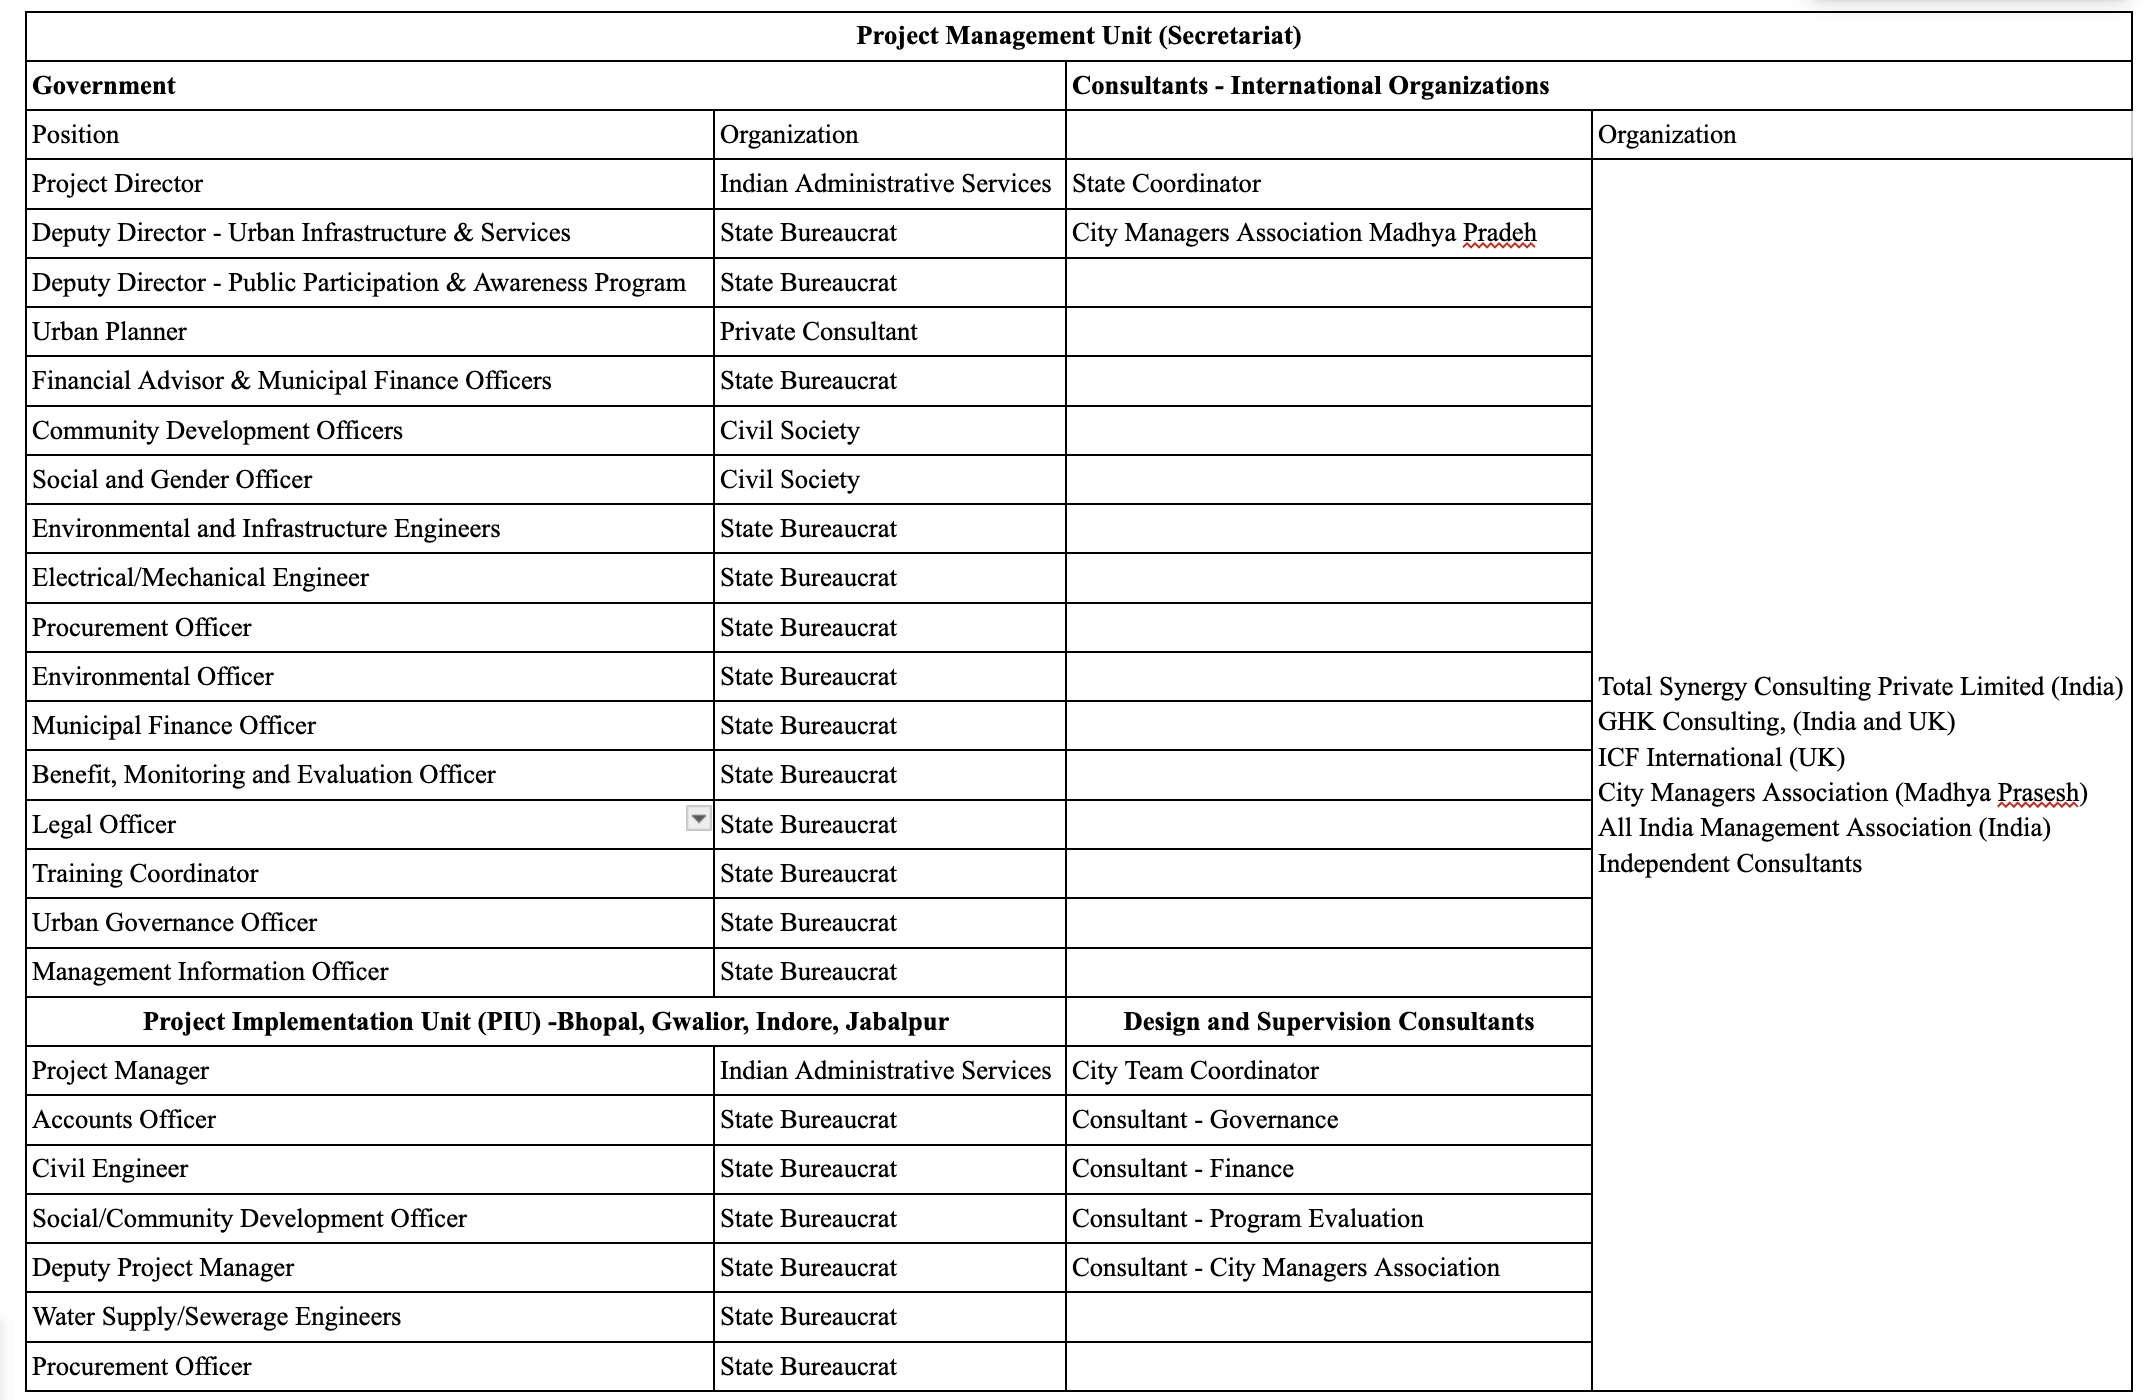
\includegraphics[width=1\textwidth]{images/ORGANOGRAM.png} % Adjust the width as needed
    \caption{Organogram under the Project Management Unit and Project Implementation Unit - 2005-2016. Source Primary Field work and \url{https://web.archive.org/web/20180829001059/http://projectuday.gov.in/Organisation.htm}}
   
\end{figure}

\subsection{Results from Citizen Survey}

The quantitative analysis of water access in Bhopal and Lucknow, drawn from the city-representative survey (n=3,754), provides compelling evidence of both city-level disparities and the critical role of political networks. The logistic regression results show that residents of Lucknow are at a distinct disadvantage compared to those in Bhopal when it comes to accessing water services. Specifically, the regression coefficient for the city dummy variable is -0.830, which translates to significantly lower odds of receiving water. When converted into odds ratios, this finding reveals that residents in Lucknow face a 56\% reduction in odds relative to Bhopal, controlling for other socio-economic and political factors (Table).  

The analysis also underscores the profound influence of political networks on water access. The regression indicates that knowing a politician personally increases the odds of receiving water, with the coefficient 0.882 translating into an odds ratio of 2.42. In other words, residents who have connections to politicians are more than twice as likely to secure water services as those without such ties. This result is further clarified by the predicted margins plot, which offers an intuitive understanding of the probabilities (Figure). For residents in Lucknow, the likelihood of receiving water remains low—around 45\%—for those who do not have any political connections. However, this probability increases sharply to approximately 88\% for individuals who know a politician personally. The nearly 43 percentage point difference highlights the systemic advantage conferred by political patronage.  

Together, these findings reveal a deeply politicized landscape of water provisioning in Lucknow, where access is shaped not just by infrastructural constraints but by one's position within political networks. 


\begin{table}[H]
\centering
\footnotesize  % This reduces the table size by approximately 1 point
\caption{Regression Results for Water in Bhopal and Lucknow}
\begin{tabular}{lD{.}{.}{-1}D{.}{.}{-1}D{.}{.}{-1}}
\toprule
\textbf{Independent Variables} & \multicolumn{1}{c}{\textbf{Full Sample}} & \multicolumn{1}{c}{\textbf{Bhopal}} & \multicolumn{1}{c}{\textbf{Lucknow}} \\
\midrule
City Dummy: Lucknow        & -0.830^{***}  &     &     \\
                           & (0.0852)      &     &     \\
Religion: Muslim           & -0.149^{*}    & 0.137       & -0.258^{**} \\
                           & (0.0858)      & (0.132)     & (0.127)     \\
Caste: OBC                 & -0.0281       & 0.148       & -0.125      \\
                           & (0.0801)      & (0.127)     & (0.111)     \\
Caste: SC                  & -0.367^{***}  & -0.315^{*}  & -0.399^{**} \\
                           & (0.118)       & (0.170)     & (0.182)     \\
Assets                     & 0.347^{***}   & -0.160      & 0.878^{***} \\
                           & (0.0775)      & (0.114)     & (0.110)     \\
Political Engagement Beyond Voting & -0.154 & 0.228       & -0.502^{***} \\
                           & (0.113)       & (0.205)     & (0.156)     \\
Effective Number of Parties & -0.197^{***} & -0.0594     & -0.268^{***} \\
                           & (0.0410)      & (0.0867)    & (0.0508)    \\
Know a Bureaucrat Personally & -0.236^{***} & -0.0831     & -0.129      \\
                           & (0.0891)      & (0.130)     & (0.132)     \\
Know a Politician Personally & -0.0234      & -1.072^{***}& 0.882^{***} \\
                           & (0.145)       & (0.202)     & (0.207)     \\
Know Both Personally        & 0.178        & -0.189      & 0.407^{**}  \\
                           & (0.140)       & (0.303)     & (0.165)     \\
Constant                    & 0.992^{***}  & 1.994^{***} & -0.158      \\
                           & (0.231)       & (0.400)     & (0.363)     \\
\midrule
Observations                & \multicolumn{1}{c}{3,754} & \multicolumn{1}{c}{1,888} & \multicolumn{1}{c}{1,866} \\
\midrule
AIC                         & \multicolumn{1}{c}{1.224} &     &     \\
BIC                         & \multicolumn{1}{c}{-11592.766} &     &     \\
Log-Lik Full Model          & \multicolumn{1}{c}{-1110.05} &     &     \\
LR(22)                      & \multicolumn{1}{c}{281.179} &     &     \\
Prob \succ R                   & \multicolumn{1}{c}{0} &     &     \\
Adj Count R2                & \multicolumn{1}{c}{0.138} &     &     \\
\bottomrule
\end{tabular}
\vspace{1em}  % Adds vertical space between the table and the footnote
\caption*{\footnotesize Robust standard errors in parentheses. \\ *** p\textless 0.01, ** p\textless 0.05, * p\textless 0.1.}
\end{table}

\begin{figure}[H] % Use [H] to force the image to appear exactly where you place it
    \centering
    \includegraphics[width=1\textwidth]{images/Networks_water.png} % Adjust the width as needed
    \caption{This figure illustrates the predicted marginal effects of network connections
on access to water services for residents in Bhopal (blue circles) and Lucknow (orange
squares). The Y-axis represents the predicted margins (likelihood of receiving water ser-
vices), while the X-axis categorizes respondents based on their network connections. The
error bars represent 95\% confidence intervals.Source: Primary survey under the Brown - India Citizenship Project 2022}
   
\end{figure}





\chapter{Bureaucratic Coordination in Trash Management: Evidence from Bhopal and Lucknow}

This chapter investigates the critical role of bureaucratic capacity in the provision of public goods within rapidly urbanizing societies, focusing on the cities of Bhopal and Lucknow. It argues that the effectiveness of public service delivery in these urban contexts is determined not just by overcoming social cohesion challenges but by the institutional configuration and capacity of state structures. Through a detailed analysis of Bhopal, the chapter shows how state-level bureaucrats enhance governance by effectively managing horizontal and vertical coordination, acting as boundary spanners, and leveraging institutional knowledge. In contrast, Lucknow's fragmented approach underscores the challenges posed by weaker bureaucratic frameworks. This comparative analysis underscores the importance of robust bureaucratic structures and strategic coordination in shaping state capacity and ensuring the equitable delivery of public services in diverse urban environments.

\section{Why study trash?}

Trash embodies the classical characteristics of a public good: non-excludability and non-rivalry \citep{Samuelson1954, Bennett1979}. Once waste management services are implemented, it is impractical to exclude individuals from their benefits, and one person's use does not diminish the availability of the service to others. This inherent nature necessitates governmental oversight to ensure equitable access and the overall welfare of the community. Concurrently, trash management serves as a tangible indicator of state capacity and legitimacy \citep{Fukuyama2013}. Though often perceived as a mundane aspect of daily life, trash collection reveals much about how governments operate and manage public services, reflecting the state's ability to implement policies, maintain public health, and manage resources effectively.

By efficiently organizing and delivering these essential services, governments fulfill their fundamental role in upholding public health and environmental standards while reinforcing the social contract with citizens. The visibility and universality of waste management makes it a critical area for public accountability, where performance directly impacts public satisfaction and, by extension, political stability \citep{Peters2016}.

Moreover, the study of trash collection highlights the critical role played by the ``hidden state''— local governments—in developing state capacity and providing essential public services. While often overlooked in favor of federal agencies and national policies, local governments are where the state truly meets the street \citep{Zacka2017}. Focusing on the local state allows for a deeper appreciation of the importance of local political dynamics, public-private partnerships, and the agency of actors at the margins in shaping political development. This bottom-up perspective reveals the complex and often contradictory processes through which state capacity is built and exercised.

In the case of India, described as ``weak-strong'' \citep{Rudolph1987}, ``failed developmental'' \citep{Herring1999}, ``Sisyphean'' \citep{Kapur2007} and ``flailing'' \citep{Pritchett2009} the study of trash management provides a case to untangle the mechanisms behind these characterizations. Bhopal and Lucknow are presented as ``critical cases'' \citep{Eckstein1975} for examining urban state capacity. A critical case permits analytic generalization: if a theory proves effective in the challenging conditions of a critical case, it is likely to succeed in less challenging or more typical conditions as well. These two cities, situated in the so-called 'BIMARU' states—characterized by low Human Development Index (HDI) and poor state capacity—represent a rigorous test for theories of state efficacy and institutional performance.

There is also the critical question of how much power an Indian city actually wields. Indian cities operate with a severely limited scope of authority, primarily managing tasks such as trash collection, issuing birth and death certificates, and maintaining burial grounds (Annexure-1). More significant functions, such as land use and planning, often remain under the control of para-state bodies, while even basic municipal functions like sanitation, roads, street lighting, and sewerage are only selectively delegated to city governments or shared among various agencies, creating a complex web of line bureaucracies with their own chains of command. In this context, studying trash collection and management becomes an essential lens for understanding the true functioning and capacity of the urban local state in India. It is also important to note that, by law, bureaucrats in Indian cities often possess more power than elected officials. This structural feature makes urban centers a particularly relevant focus for examining bureaucratic state capacity. If there is a case to be made for studying bureaucratic state capacity, it must begin with the cities.

\section{Descriptive Statistics and Data}

\subsection{Demographic and Administrative Data}

Table \ref{tab:admin_data} provides a comparative overview of demographic and socio-economic indicators for the two cities. Table \ref{tab:admin_structure} compares the governance frameworks of the two cities. It shows that both cities have directly elected mayors and indirectly elected city councils, with commissioners serving as the administrative heads. However, Bhopal has more autonomy, with six powers under the independent control of the city government, compared to just one in Lucknow.

\begin{table}[ht]
\centering
\caption{Administrative Data Comparison: Bhopal and Lucknow}
\label{tab:admin_data}
\begin{tabular}{|l|c|c|c|c|c|c|c|c|}
\hline
\textbf{City} & \textbf{Area} & \textbf{Population} & \textbf{Slum} & \textbf{Literacy} & \textbf{SC} & \textbf{OBC} & \textbf{Forward} & \textbf{Muslim} \\
 & \textbf{(sq. km.)} & \textbf{(2011)} & \textbf{\%} & \textbf{\%} & \textbf{\%} & \textbf{\%} & \textbf{\%} & \textbf{\%} \\
\hline
Bhopal & 286 & 1798218 & 26.68 & 83 & 14.36 & 39.98 & 42.70 & 24.69 \\
\hline
Lucknow & 349 & 2817105 & 12.95 & 86 & 10.79 & 42.26 & 43.83 & 21.79 \\
\hline
\end{tabular}
\raggedright
\small Source: Census of India 2011. The OBC, Forward caste numbers are from Brown Citizen Urban Survey
\end{table}

\begin{table}[ht]
\centering
\caption{Administrative Structure of the City Governments: Bhopal and Lucknow}
\label{tab:admin_structure}
\begin{tabular}{|l|c|c|c|c|c|}
\hline
\textbf{City} & \textbf{Mayor} & \textbf{City Council} & \textbf{Administrative} & \textbf{Powers under} & \textbf{Municipal} \\
 & & & \textbf{Head} & \textbf{independent control*} & \textbf{Budget} \\
\hline
Bhopal & Directly Elected & Indirectly Elected & Commissioner & 6 & \$26.00 bn \\
\hline
Lucknow & Directly Elected & Indirectly Elected & Commissioner & 1 & \$28.65 bn \\
\hline
\end{tabular}
\raggedright
\small *Solid waste management is common for the two cities.\\
\small Bhopal has solid waste management, fire services, urban poverty alleviation, urban amenities and facilities, burials and crematoriums. Cattle pounds, birth and death, bus stop.\\
\small Source: Respective State Municipal Acts and Budget Documents
\end{table}

\subsection{Descriptive Results from Survey Data}

The data used in this study comes from the Brown University - Urban Citizenship Survey, a face-to-face survey conducted between May and June 2022. The survey aimed to collect data on urban citizenship, across multiple cities. The sample includes 4,230 respondents. While a more detailed treatment of the data, including multivariate analysis, will be addressed in a subsequent chapter, this section focuses on providing specific observations related to disparities in waste management services.

Question asked: What is the frequency of trash collection at your house?

Table \ref{tab:trash_collection} shows that overall, Bhopal demonstrates a more systemized waste collection process, with 76.3\% of households receiving daily trash pickup, compared to only 48.63\% in Lucknow. This regularity highlights Bhopal's effective service. In contrast, Lucknow shows significant inconsistency, with 12.04\% of households reporting that their trash is never collected, indicating a higher number of households in Lucknow face inadequate waste management compared to Bhopal.

\begin{table}[ht]
\centering
\caption{Overall distribution of frequency of trash collection: City Level}
\label{tab:trash_collection}
\begin{tabular}{|l|c|c|}
\hline
\textbf{Frequency} & \textbf{Bhopal} & \textbf{Lucknow} \\
\hline
More than once a day & 11.71 & 16.82 \\
\hline
Once a day & 76.3 & 48.63 \\
\hline
Several times a week & 6.18 & 17.3 \\
\hline
Once a week & 2.47 & 2.32 \\
\hline
Less frequently than once a week & 0.87 & 1.66 \\
\hline
Never & 2.1 & 12.04 \\
\hline
Don't Know & 0.32 & 0.47 \\
\hline
Refused to answer & 0.05 & 0.76 \\
\hline
\end{tabular}
\end{table}

Tables \ref{tab:trash_caste_lucknow} and \ref{tab:trash_caste_bhopal} show significant disparities in trash collection across caste groups in Lucknow, while Bhopal exhibits more consistent service across all groups. In Bhopal, trash collection is uniform, with all caste groups receiving similar rates of daily pickup (around 74\% to 78\%), indicating an inclusive service that does not exclude any particular group.

However, in Lucknow, there is a pronounced disparity, especially among SC groups.\footnote{ST sample is excludable because of the small sample size.} A substantial 27.48\% of SCs and 51.92\% of STs report that their trash is never collected, highlighting severe inequities in service provision. Additionally, the SC and OBC groups in Lucknow exhibit a bimodal distribution: some households report that trash is never picked up, while others receive collection more than once a day. This trend is particularly stark among SC households, suggesting that while some benefit from frequent service, a significant number are completely neglected. This pattern points to a systemic issue in Lucknow's waste management, where marginalized communities, especially SCs and STs, face inconsistent and often inadequate service.

It could be that this pattern reflects the influence of networks; those who receive frequent service might be connected through networks established by successive SP and BSP governments, which historically provided jobs and access to these groups. This suggests that waste collection in Lucknow may be rationed, with access to services potentially dependent on these networks, leaving those without connections underserved.

\begin{table}[ht]
\centering
\caption{Distribution of frequency of trash collection by caste: Lucknow}
\label{tab:trash_caste_lucknow}
\begin{tabular}{|l|c|c|c|c|c|}
\hline
\textbf{Frequency} & \textbf{OBC} & \textbf{SC} & \textbf{ST} & \textbf{Gen} & \textbf{Overall} \\
\hline
More than once a day & 15.49 & 23.87 & 5.77 & 16.96 & 16.82 \\
\hline
Once a day & 51.14 & 31.98 & 30.77 & 51.55 & 48.63 \\
\hline
Several times a week & 15.83 & 11.26 & 3.85 & 21.06 & 17.3 \\
\hline
Once a week & 3.3 & 2.25 & 0 & 1.66 & 2.32 \\
\hline
Less frequently than once a week & 1.71 & 0.45 & 1.92 & 1.88 & 1.66 \\
\hline
Never & 11.5 & 27.48 & 51.92 & 6.54 & 12.04 \\
\hline
Don't Know & 0.34 & 0.9 & 1.92 & 0.33 & 0.47 \\
\hline
Refused to answer & 0.68 & 1.8 & 3.85 & 0 & 0.76 \\
\hline
\end{tabular}
\end{table}

\begin{table}[ht]
\centering
\caption{Distribution of frequency of trash collection by caste: Bhopal}
\label{tab:trash_caste_bhopal}
\begin{tabular}{|l|c|c|c|c|c|}
\hline
\textbf{Frequency} & \textbf{OBC} & \textbf{SC} & \textbf{ST} & \textbf{Gen} & \textbf{Overall} \\
\hline
More than once a day & 12.17 & 8.97 & 16.39 & 12.4 & 11.71 \\
\hline
Once a day & 77.09 & 74.09 & 78.69 & 75.87 & 76.3 \\
\hline
Several times a week & 5.25 & 9.97 & 0 & 6.03 & 6.18 \\
\hline
Once a week & 2.63 & 2.66 & 4.92 & 2.01 & 2.47 \\
\hline
Less frequently than once a week & 0.95 & 1.33 & 0 & 0.78 & 0.87 \\
\hline
Never & 1.31 & 2.99 & 0 & 2.79 & 2.1 \\
\hline
Don't Know & 0.48 & 0 & 0 & 0.11 & 0.32 \\
\hline
Refused to answer & 0.12 & 0 & 0 & 0 & 0.05 \\
\hline
\end{tabular}
\end{table}

The pattern observed in caste-based disparities is mirrored in the religious distribution of trash collection services, although the differences are smaller. In Bhopal, both Hindus and Muslims receive equal service, with similar rates of daily trash collection and low percentages of households reporting that their trash is never collected. This indicates that no religious group is particularly excluded from service in Bhopal.

In contrast, Lucknow shows notable disparities, though less pronounced than those seen in caste-based data. A higher percentage of Muslims (14.38\%) report that their trash is never collected compared to Hindus (10.66\%), and fewer Muslim households (8.5\%) receive trash collection more than once a day, compared to Hindus (18.63\%). This suggests that Muslim communities in Lucknow may be receiving less frequent and less reliable waste management services, possibly as a result of selective distribution practices. However, it's important to note that these religious differences in service access are not as stark as those observed across caste groups.

\begin{table}[ht]
\centering
\caption{Distribution of frequency of trash collection by Religion: Lucknow}
\label{tab:trash_religion_lucknow}
\begin{tabular}{|l|c|c|c|}
\hline
\textbf{Frequency} & \textbf{Hindu} & \textbf{Muslim} & \textbf{Overall} \\
\hline
More than once a day & 18.63 & 8.5 & 16.82 \\
\hline
Once a day & 48.69 & 51.2 & 48.63 \\
\hline
Several times a week & 17.42 & 18.74 & 17.3 \\
\hline
Once a week & 2.04 & 3.05 & 2.32 \\
\hline
Less frequently than once a week & 1.15 & 3.49 & 1.66 \\
\hline
Never & 10.66 & 14.38 & 12.04 \\
\hline
Don't Know & 0.45 & 0.44 & 0.47 \\
\hline
Refused to answer & 0.96 & 0.22 & 0.76 \\
\hline
\end{tabular}
\end{table}

\begin{table}[ht]
\centering
\caption{Distribution of frequency of trash collection by Religion: Bhopal}
\label{tab:trash_religion_bhopal}
\begin{tabular}{|l|c|c|c|}
\hline
\textbf{Frequency} & \textbf{Hindu} & \textbf{Muslim} & \textbf{Overall} \\
\hline
More than once a day & 11.87 & 10.78 & 11.71 \\
\hline
Once a day & 76.51 & 75.46 & 76.3 \\
\hline
Several times a week & 6.22 & 6.13 & 6.18 \\
\hline
Once a week & 2.83 & 1.67 & 2.47 \\
\hline
Less frequently than once a week & 0.94 & 0.74 & 0.87 \\
\hline
Never & 1.26 & 4.83 & 2.1 \\
\hline
Don't Know & 0.38 & 0.19 & 0.32 \\
\hline
Refused to answer & 0 & 0.19 & 0.05 \\
\hline
\end{tabular}
\end{table}

The data reveals contrasting waste management scenarios in Bhopal and Lucknow. While Bhopal demonstrates equitable trash collection across caste and religious groups, Lucknow shows significant disparities. In Lucknow, SC communities are most affected, with many households never receiving trash collection, while OBCs face challenges to a lesser extent. Religious disparities are also evident, with Muslim households experiencing more service lapses than Hindu households. These inequalities may be influenced by social networks and political connections, particularly given the historical dominance of the BSP (supported by Dalits) and SP (backed by Yadavs/OBCs) in securing sanitation jobs for their constituents.

\subsection{Overview of Bureaucratic Roles and Responsibilities in Urban Governance}

Table \ref{tab:bureaucratic_roles} gives an overview of bureaucratic roles and responsibilities in these cities. In this chapter, ``central bureaucrats'' refers to officers of the Indian Administrative Services (IAS), selected through a national competitive exam. These officers often serve as city Commissioners and Secretaries to State Governments, particularly in departments like Urban Development and Housing. In Lucknow, Commissioners are drawn from both central and state bureaucracies, while in Bhopal, they are exclusively from the central bureaucracy.

``State bureaucrats'' are officers selected through state-level exams conducted by the State Public Service Commission. These officers hold positions such as Assistant, Joint, or Additional Commissioners in city governments, and may be promoted to Commissioner roles in smaller towns and cities. Bhopal's bureaucracy includes officers from the Madhya Pradesh Municipal Administration Services, a cadre dedicated exclusively to urban administration. These career bureaucrats are posted solely in urban areas. Within the city government, they operate under the authority of the City Commissioner.

``Mid-level bureaucrats'' are technical experts in fields like engineering, sanitation, and revenue. They are either appointed by city governments or through relevant state departments, ensuring the efficient operation of city services. ``Street-level bureaucrats'' manage daily administrative tasks, including processing paperwork, maintaining records, and staffing ward and zone offices. Like mid-level bureaucrats, they are appointed either by the city governments or through relevant departments. Finally, street-level workers perform essential on-the-ground tasks such as street sweeping, trash collection, and drain cleaning. They form the largest segment of the workforce and are recruited by the city or the state urban department.

\begin{table}[ht]
\centering
\caption{Overview of Bureaucratic Roles and Responsibilities in Urban Governance}
\label{tab:bureaucratic_roles}
\begin{tabular}{|p{3cm}|p{5cm}|p{3cm}|p{5cm}|}
\hline
\textbf{Category} & \textbf{Description} & \textbf{Selection Process} & \textbf{Roles/Responsibilities} \\
\hline
Central Bureaucrats (Elite Bureaucrats) & Officers from the Indian Administrative Services (IAS), selected through a national competitive exam. & Nationally competitive exam (IAS) & Serve as city Commissioners, Secretaries to State Government departments (Urban Development, Housing, ULBs, etc.). \\
\hline
State Bureaucrats & Officers selected through state-level exams conducted by the State Public Service Commission. & State Public Service Commission exam & Hold positions such as Assistant, Joint, or Additional Commissioners in city governments, potential promotion to Commissioner. \\
\hline
Mid-Level Bureaucrats & Technical experts in fields such as engineering, sanitation, and revenue. & Appointed by city governments or relevant state departments & Provide technical expertise for efficient city operations. \\
\hline
Street-Level Bureaucrats & Handle day-to-day administrative tasks such as processing paperwork, maintaining records, and staffing ward and zone offices. & Appointed by city governments or relevant state departments & Manage daily administrative functions within city governments. \\
\hline
Street-Level Workers & Employees responsible for essential tasks like street sweeping, trash collection, drain cleaning, and operating waste management machinery. & Appointed by city governments or relevant state departments & Perform on-the-ground tasks essential for city cleanliness and public health. \\
\hline
\end{tabular}
\end{table}

\begin{figure}[ht]
\centering
\caption{Map of Lucknow City by Wards – Field Sites Highlighted in Color}
\label{fig:lucknow_map}
% Insert the figure here
\end{figure}

\begin{table}[ht]
\centering
\caption{Field Sites in Lucknow}
\label{tab:field_sites_lucknow}
\begin{tabular}{|p{2.5cm}|p{5cm}|p{6cm}|}
\hline
\textbf{Ward} & \textbf{Trash Collection} & \textbf{Rationale} \\
\hline
Aliganj & ``Contractor'' and city empaneled private concessionaire & Older Development - Salaried Class, Middle Class, Planned Colony \\
\hline
Gomti Nagar & City empaneled private Concessionaire & New Development - Upper Middle Class, Commercial establishments \\
\hline
Hazratganj & ``Contractor'' & Old Development - Significant Muslim population \\
\hline
Transport Nagar & ``Contractor'' and city empaneled private concessionaire & New Development - Migrant population, Dalits and Muslims from Bihar and Eastern Uttar Pradesh \\
\hline
\end{tabular}
\end{table}

\section{Lucknow}

In Lucknow, the elected local politicians, known as councilors, possess limited policy making power, resulting in a role that is primarily administrative rather than policy focused. Operating in a politically fragmented society where various social groups act as core patrons of political parties these politicians find themselves with little choice but to distribute patronage due to their inability to influence policy. Central politicians, who control the career incentives of Lucknow's bureaucracy, exert significant pressure on bureaucrats to comply with specific demands, aligning bureaucratic actions with political interests rather than the public good.

Consequently, trash management, being both a major employer and responsibility of the councilors, becomes a focal point for local political actors to assert their legitimacy and satisfy their patrons. Given limited city resources and the pressures from their respective patron groups, both local and elite politicians influence bureaucrats, compelling them to comply with their demands. This leads to the marginalization of the bureaucracy's capacity to pursue systemic reforms. Central bureaucrats cannot monitor their subordinates and consequently, align their career incentives with elite political leaders.

When faced with potential sanctions or reforms, lower and mid-level bureaucrats reach beyond their immediate superiors, leveraging external political connections and interdepartmental alliances. As a result, the local state chooses to privatize trash management, but that too is met with challenges. The private concessionaires are caught in the middle, navigating between local politicians, who prioritize patronage over efficient service delivery, and a constrained bureaucracy that lacks the capacity for coordination. This situation results in a failure to provide effective services.

Consequently, trash management in Lucknow highlights a scenario where fragmented societal structures shape the politician-bureaucrat relationship, ensuring that no group is entirely excluded from services. Nevertheless, the quality of these services remains substandard, impeding the development of a cohesive, city-wide system.

\subsection{Lucknow - Politics and Administration}

\subsubsection{The State}

Uttar Pradesh (UP) has been the epicenter of ``Mandal politics'' – a socio-political movement in India focused on advocating for caste-based reservations and representation.\footnote{The term ``Mandal politics'' originates from the Mandal Commission, established in 1979, which recommended reserving a significant percentage of government jobs and educational institution seats for OBCs. This movement has been central to debates on social justice, caste representation, and the political mobilization of historically disadvantaged groups in India.} This gave rise to two regional powerhouses: the Bahujan Samaj Party (BSP), championing Dalit rights, and the Samajwadi Party (SP), representing OBCs and Muslims \citep{Pai2013}.\footnote{While parties in Uttar Pradesh, as in most First-Past-the-Post systems, must build broad-based coalitions to secure electoral victories, their core support and political identity remain strongly tied to specific social groups.} These regional forces vie for political control alongside national parties like the Bharatiya Janata Party (BJP) and the Indian National Congress who's political core are the residual caste groups.\footnote{The BJP builds alliances among the non-Yadav OBC and forward castes, particularly the Rajputs whereas Congress has been traditionally seen as the party of the Brahmins.} In the 65-year history of the state, only in the last two decades have the governments completed full terms.\footnote{In the history of the state, only three Chief Ministers have completed full terms, all within this recent period. Mayawati of the Bahujan Samaj Party (BSP) served from 2007 to 2012, followed by Akhilesh Yadav of the Samajwadi Party (SP) from 2012 to 2017, and currently, Yogi Adityanath of the BJP since 2017.} The city also is a ``VIP'' seat having elected the three-term Prime Minister Atal Bihari Vajpayee (Member of Parliament from 1991 to 2009) and the current Defense Minister, a former chief of the BJP (Member of Parliament from 2014-now).

With only 22\% urbanization rate, UP has the lowest urban populations (and the highest rural population) in the country.\footnote{Census of India. (2011). Census of India 2011: Final population totals. Office of the Registrar General \& Census Commissioner, India.} This rural dominance is reflected in political representation: only 4 out of 80 parliamentary constituencies and 40 out of 403 state assembly constituencies are urban.\footnote{Computed from the Global Human Settlement layer, 2022 release. Shapefiles for the parliamentary and assembly constituencies are collected from Datameet. I considered urban centers, dense urban areas, and semi dense urban areas within a constituency as a proxy of urbanization. For methodology to formulate these categories, please see https://human-settlement.emergency.copernicus.eu/documents/GHSL\_Data\_Package\_2023.pdf?t=1716923464.} Consequently, state politicians often extract rents from cities to support activities in rural areas, explaining the underinvestment in urban areas compared to rural ones \citep{Varshney1995}.

The Dalit-supported BSP invested heavily in constructing parks across the state, including Lucknow \citep{Heath2012}. The SP focused on marquee projects like riverfront development, eight lane expressways and metro systems\footnote{Infrastructure to social development: Tracing shift in Samajwadi Party.'' Hindustan Times. March 11, 2024.} and the current BJP government is seen to invest in creating temple corridors.\footnote{Even though the Clean India campaign got a big push under the BJP, UP cities have consistently ranked the lowest in cleanliness rankings.} Focus on the fundamental infrastructure - water supply, public transport, waste management has received low priority. Lucknow's bargaining power is minimal, relegating its priorities to the bottom of the state's agenda. A IAS office in the state Secretariat candidly admitted:

``I am not ashamed to say this: everyone has used the municipality as a toolkit. Municipal ka shoshan pura administration karta hai (Municipal administration is exploited by the entire administrative system).''\footnote{Interview with Arvind Kumar Giri, Under Secretary, Uttar Pradesh. Lucknow 2022}

Administratively, Lucknow's governance structure is different from most Indian cities. The position of Commissioner in the Lucknow City Government (LMC) has been occupied by both Indian Administrative Service (IAS) officers and Provincial Civil Service (UP-PCS) officers. PCS officers are subordinate to the IAS officers in the administrative hierarchy. In contrast to most Indian cities, especially state capitals, where IAS officers typically serve as Commissioners, Lucknow only saw PCS officers in this role (until most recently). These PCS officers were more beholden to state interests, as evidenced by recent appointment patterns in Lucknow. From 1999 to 2024, Lucknow has seen 29 city commissioners. Of these 29, only five commissioners have had tenure longer than two years while 24 commissioners had an average tenure of just over six months. The tenures of the longest serving commissioners were co-terminus with the government which appointed them (Table \ref{tab:commissioner_tenures}).

\begin{table}[ht]
\centering
\caption{Recent Tenures of Municipal Commissioners of Lucknow}
\label{tab:commissioner_tenures}
\begin{tabular}{|p{4cm}|c|p{5cm}|c|}
\hline
\textbf{Party in power} & \textbf{Tenure} & \textbf{Commissioner, Lucknow City} & \textbf{Tenure} \\
\hline
Bahujan Samajwadi Party & 2007-2012 & Mr. Shailesh Kumar Singh (PCS) & 2007-2012 \\
\hline
Samajwadi Party & 2012-2017 & Mr. Udayraj Singh (PCS) & 2013-2017 \\
\hline
\multirow{2}{*}{Bharatiya Janata Party} & \multirow{2}{*}{2017-2022} & Dr. Indramani Tripathi (PCS) & 2018-2021 \\
\cline{3-4}
 & & Ajay Kumar Dwiwedi (IAS) & 2021-2023 \\
\hline
Bharatiya Janata Party & 2022-now & Inderjeet Singh (IAS) & 2023-now \\
\hline
\end{tabular}
\raggedright
\small Source: Lucknow City Government website
\end{table}

\subsubsection{The City}

Lucknow's social group includes Muslims, upper castes, OBCs, and others. Although these groups are not numerically equal, each represents a significant portion, resulting in a pluralistic demographic landscape (see Table \ref{tab:admin_data}). Social groups closely aligned with political parties as evidenced by the results of the last city election. All Muslim councilors were elected on the SP ticket, 82\% councilors in the Dalit reserved wards belonged to the BSP, and the majority of unreserved wards were won by the BJP (Table \ref{tab:political_composition}). The large forward caste population in Lucknow partly explains the BJP's dominance in the Mayoral position, which it has consistently held since 2006. Despite the limited functional power of the LMC, the political arena has been hotly contested, evidenced by the lack of a single-party majority in city elections until 2017.

\begin{table}[ht]
\centering
\caption{Political Composition of Lucknow Municipal Corporation and Corresponding State and National Governments (2000-Present)}
\label{tab:political_composition}
\begin{tabular}{|c|c|c|c|c|}
\hline
\textbf{Tenure} & \textbf{Mayor} & \textbf{Lucknow Municipal Corporation} & \textbf{State} & \textbf{National} \\
\hline
2002-2006 & Administrator & Divided - no majority & SP/BSP & NDA/UPA \\
\hline
2006 -2012 & BJP & Divided - no majority & BSP & UPA \\
\hline
2012-2017 & BJP & Divided - no majority & SP & UPA/NDA \\
\hline
2017-2023 & BJP & BJP & BJP & NDA \\
\hline
2023 - now & BJP & BJP majority & BJP & NDA \\
\hline
\end{tabular}
\raggedright
\small NDA - BJP led National Democratic Alliance, UPA - Congress led United Progressive Alliance\\
\small Source: State Election Commission for Mayor and City Government and Election Commission of India for the State Election
\end{table}

In contrast to the state and national levels, where representation for groups such as Muslims and Scheduled Castes is minimal or absent, city governments provide a more inclusive political arena. Table \ref{tab:representation} illustrates the significant gap between local-level representation and higher political offices. While Muslims make up 26\% of Lucknow's population and hold 13\% of the wards in the Lucknow Municipal Corporation (LMC), they have no representation in the State Assembly or Parliamentary constituencies covering Lucknow city. The same is true for Dalits. This disjunction between local and higher-level political representation positions the local state as a unique site for representation, particularly for marginalized communities. A city ward— the electoral unit of the LMC, characterized by a small, concentrated population—allows for better representation, enabling even marginalized groups to exert influence disproportionate to their overall population share. The local state, therefore, becomes a critical site for the expression and negotiation of group identities and interests, significantly impacting politicians in Lucknow who seek to remain competitive and secure election victories.

\begin{table}[ht]
\centering
\caption{Representation of Muslims and Scheduled Castes in Lucknow's Population, City government, and Legislative Bodies (2018-2023)}
\label{tab:representation}
\begin{tabular}{|l|c|c|}
\hline
\textbf{Level of Governance} & \textbf{Muslims} & \textbf{Scheduled Castes} \\
\hline
Population & 26\% & 10\% \\
\hline
Lucknow city government (LMC) & 13\% & 12\% \\
\hline
MLA (Assembly constituencies which form part of Lucknow) & Nil & Nil \\
\hline
MP (Parliamentary constituencies which form part Lucknow) & Nil & Nil \\
\hline
\end{tabular}
\raggedright
\small Note: The MLAs and MPs are during the fieldwork period from 2018-2023. 7 Assembly constituencies form part of Lucknow city: Bakshi Kaa Talab, Sarojini Nagar, Lucknow West, Lucknow North, Lucknow East, Lucknow Central, Lucknow Cantt. 2 Parliamentary constituency forms part of Lucknow city - Mohanlalganj PC in part, Lucknow PC in full.\\
\small Source: State Election Election Commission, Uttar Pradesh for Lucknow city data and Election Commission of India for Parliamentary and Assembly constituency data. City equivalent ACs and PCs have been derived from Delimitation of Constituencies Paper 6 and 7. Election Commission of India. Available at: https://www.eci.gov.in/delimitation
\end{table}

Lucknow exhibits significantly higher rates of non-voting political engagement compared to Bhopal, with more than double the proportion of residents holding political party memberships (Table \ref{tab:political_engagement}). This heightened political activity transforms the city into a dynamic political arena where politicians must be vigilant in guarding their territories. In the context of weak state institutions, political affiliation becomes the primary means of negotiating access to resources, further intensifying the competition among politicians to secure and deliver tangible benefits to their constituents. The strong representation of the city's diverse social groups, coupled with elevated levels of non-voting participation, means that politicians are compelled to deliver resources and services to remain competitive. The absence of formal deliberative forums in the city exacerbates this dynamic, as politicians, pressured to meet the demands of their politically active base, exert influence over bureaucrats to secure the delivery of public goods. This need to respond quickly and effectively to their constituencies' demands undermine more systematic and long-term approaches to governance, including better trash management.

\begin{table}[ht]
\centering
\caption{Political Engagement in Lucknow and Bhopal by Social Group}
\label{tab:political_engagement}
\begin{tabular}{|l|l|c|c|c|c|}
\hline
\textbf{City} & \textbf{Group} & \textbf{Time Contributed} & \textbf{Participated} & \textbf{Discussed Supporting} & \textbf{Political Party} \\
 & & \textbf{to Campaigns (\%)} & \textbf{in Rallies (\%)} & \textbf{a Candidate (\%)} & \textbf{Member (\%)} \\
\hline
\multirow{5}{*}{Lucknow} & City & 23.51 & 22.32 & 23.51 & 17.39 \\
\cline{2-6}
 & Muslims & 20.48 & 19.17 & 24.18 & 15.03 \\
\cline{2-6}
 & Hindus & 25.34 & 24.12 & 24.12 & 18.89 \\
\cline{2-6}
 & SC & 19.82 & 18.47 & 16.67 & 12.16 \\
\cline{2-6}
 & OBC & 26.08 & 25.28 & 26.08 & 19.36 \\
\cline{2-6}
 & Forward & 3.61 & 22.28 & 24.72 & 18.40 \\
\hline
\multirow{6}{*}{Bhopal} & City & 12.81 & 8.78 & 10.02 & 6.95 \\
\cline{2-6}
 & Muslims & 17.29 & 11.34 & 13.01 & 9.11 \\
\cline{2-6}
 & Hindus & 11.43 & 7.98 & 9.11 & 6.22 \\
\cline{2-6}
 & SC & 11.63 & 5.98 & 7.97 & 3.65 \\
\cline{2-6}
 & OBC & 13.60 & 9.43 & 10.38 & 5.49 \\
\cline{2-6}
 & Forward & 13.63 & 10.39 & 11.73 & 9.61 \\
\hline
\end{tabular}
\raggedright
\small The shares refer to the percentage of respondents within each social group who have said 'yes' to questions on political participation.\\
\small Source: Brown - India Citizen Urban Survey 2022
\end{table}

\subsection{Politics and Reform Resistance}

This section examines how Lucknow's fragmented political landscape influences trash management. It demonstrates that the divided social base is associated with politicians at various levels restricting bureaucratic action. The analysis highlights two key points: the persistence of patronage in waste management and resistance to reforms. These dynamics support earlier arguments that competitive representation among social groups contributes to patronage-based service delivery and reform resistance, ultimately maintaining existing power structures. The local political arena thus becomes a crucial space for identity expression and resource negotiation, often at the expense of efficient, city-wide governance.

At the street level, local councilors have maintained a tight grip on the recruitment process for crucial services such as trash collection and street sweeping. Their control over hiring practices persisted even after privatization.\footnote{Lucknow privatized its trash management in 2010 - after which it hired two concessionaires, all of whose contracts were terminated before time. More on this is discussed later.} In the early 2000s, Lucknow was no different from other Indian cities in terms of its trash management. One of the longest serving councilor of the Lucknow city government in an interview told me:

``Trash was not even something that we thought of as needing scientific solutions. In the new areas, there was some collection and disposal, but here, most of the councilors had to handle this issue. They would get their local people. It worked both ways - it gave their people employment, and got the area cleaned.''\footnote{Interview with current leader of the opposition in the Lucknow city corporation Syed Yawar Hussain Reshu, Lucknow 2022.}

In 2004, the Indian government launched the Jawaharlal Nehru National Urban Renewal Mission (JnNURM), allocating \$14 billion for urban development. This program tied funding to governance reforms, incentivizing states and cities to implement specific policies and demonstrate results to access the funds.\footnote{JNNURM established two channels for intervention: Urban Infrastructure and Governance (UIG), funding city-wide infrastructure like water supply, sewerage, urban transport, and solid waste management; and Basic Services for the Urban Poor (BSUP), targeting housing, water supply, and sanitation for the poor. Other vital sectors such as health, education, and social services fell outside its scope.} The same year, a coalition government of the BSP and the SP in the state pushed for Lucknow city government to open up hiring for sanitation workers and lower municipal bureaucracy.\footnote{Interview with Dr. P. K. Trivedi \& Dr. Shikha Singh, Giri Institute of Development Studies, Lucknow, 2022. Also read: ``When Neo-liberal Agenda Negotiates Dalit Agenda: The Case of BSP in Uttar Pradesh,'' in Trivedi, P. K. (Ed.), The Globalization Turbulence: Emerging Tensions in Indian Society (pp. 268-288). Rawat Publications.} The parties actively packed government jobs with their co-ethnics and party supporters, with the Lucknow city government being a prime target for this patronage. In Lucknow, party workers, councilors, intermediaries, and party leaders were given priority to get their ``support base'' into the LMC.\footnote{For a detailed examination of the relationship between jobs and ethnic parties, Kanchan Chandra's ``Why Ethnic Parties Succeed'' On page 85, Chandra explores how these parties leverage employment opportunities to build loyalty and support, offering a critical analysis of the political dynamics involved.} The city's bottom-heavy staff structure (5,745 out of 7,200 employees were sanitation workers) made it ideal for political patronage. While higher level positions were state-recruited, lower and street level bureaucracy along with street level workers were hired directly by the city where these jobs had minimal qualifications - just primary school education and there were no interviews.

Attempts to implement enhanced control measures over sanitation workers, including centralized attendance systems and management information systems, faced strong opposition from both bureaucrats and politicians. The first source of opposition arose from the local leaders who viewed employment in the city as one of the few avenues to secure positions for their supporters. This was particularly significant in a state where job opportunities were scarce, making government positions highly prized. Records from the LMC council meeting provide a unique view into the intersection of caste, employment, and local politics. Beni Ram Valmiki, referring to the Valmiki community, a group traditionally associated with sanitation work asked:

``Today, hiring in the Nagar Nigam is open to all castes. Traditionally, cleaning has been the occupation of my caste. How can this change be allowed? We will oppose any hiring that doesn't prioritize our community.''\footnote{Lucknow City Government meeting archives. Accessed from the Lucknow Nagar Nigam in 2021}

The assertion that certain communities should continue to perform caste-based work wasn't paradoxical; rather, it was a practical approach to ensure representation and employment in the absence of access to higher positions of power. Indeed, the administrative hierarchy even today reflects entrenched caste divisions, with upper castes predominantly occupying higher positions, while Scheduled Castes largely holding street level workers and bureaucrat's posts. Only 15\% (32 out of 212) of the officers in the LMC were Scheduled Castes (SC). While caste-wise data for sanitation workers is unavailable, it is known that the majority of the 11,200 workers come from lower caste backgrounds.\footnote{Compiled by employee names made available by the LMC. Name matching was done manually using list from the Ministry of Social Justice and Empowerment https://socialjustice.gov.in/common/76750}\footnote{Before elections, all parties make promises to Dalit groups to offer jobs in these positions. Indian Express. (2022, February 4). SP promises 40,000 jobs, hike in daily wage. Retrieved from https://indianexpress.com/article/cities/lucknow/sp-promises-40000-jobs-hike-in-daily-wage/}

In 2015, Jyoti Envirotech, a private concessionaire contracted for waste management in Lucknow, only operated in 55 out of 110 wards. The remaining wards were still managed by private contractors closely tied to local councilors and lower-level bureaucracy.\footnote{Final City Sanitation Plan for Lucknow, 2011 pg. XX} This informal division continues to date, with half the city cleaned by politician and bureaucrat-run firms, and the other half by the private concessionaire.\footnote{Hindustan Times. (2023, January 10). LMC to hire eight companies to improve Lucknow's ranking in cleanliness survey. Hindustan Times. https://www.hindustantimes.com/india-news/lmc-to-hire-eight-companies-to-improve-lucknow-s-ranking-in-cleanliness-survey-101673454369771.html} The historic Hazratganj ward exemplifies this divide, where the local councilor maintains his own sanitation team. In an interview:

``The company was only interested in managing the new area. Our area wasn't being properly serviced, so we demanded that the company withdraw and requested the Nagar Nigam to assign me 10 workers to handle the cleaning of my ward.''\footnote{Interview with Md. Saifullah, Councillor for the Yadunath Sanyal ward from 2006-2017, Lucknow 2022}

The then Additional Municipal Commissioner, PK Srivastava, acknowledged this approach, noting: ``We got the city to pay money. But given the pressure of the councilors from the old areas, we just thought of giving the contract to the local firm which we thought would do a better job.'' When pressed about whether the councilors' closeness to the then Urban Development Minister, who was Muslim, could have played a role, Srivastava smiled and cryptically responded: ``Politicians will do politics.''\footnote{Interview with PK Srivastava, Additional Municipal Commissioner LMC 2009-2013, Lucknow 2022}

The second source of opposition stemmed from the weak bureaucracy in Lucknow, forcing politicians to assume administrative roles typically handled by bureaucrats. The low capacity of the bureaucracy in Lucknow is discussed in the following section, but even quotidian tasks of filing complaints and receiving responses from the local bureaucracy, even for councilors, was difficult. In addition to not having any policy making powers (the LMC has no legislative powers) formal spaces to deliberate and sanction bureaucracy did not exist. House meetings occurred few and far between, and no mechanism for bureaucrats and politicians to work together existed.\footnote{The absence of these forums in Lucknow would make the city council meeting a display of heightened disagreements and showmanship. Of the eight meetings I attended during three years of conducting this study, only four lasted for more than an hour. In one meeting, the Commissioner threatened to kill a councilor, and in another meeting, a councilor tried to commit suicide by jumping out of the venue. While all this ruckus was occurring, no one cared about the physical infrastructure where these meetings were taking place. Amar Ujala. (2024, February 28). Ruckus in Lucknow Nagar Nigam over BJP corporator's comment. Retrieved from https://www.amarujala.com/lucknow/ruckus-in-lucknow-nagar-nigam-over-bjp-corporator-s-comment-2024-02-28} Consequently, politicians were deeply involved in the minutiae of day-to-day municipal operations. Shadowing two councilors from Gomti Nagar ward, it became apparent that their roles were primarily administrative. As one councilor candidly expressed,

``We are firefighters, trash pickers, and drain openers. That is our role (hum aag bhujane wale hai, kuda uthane wale hai, naali khulwane wale hai).''\footnote{Interview with Prithvi Gupta (BJP), councilor from Aliganj ward. Lucknow 2022}

This statement vividly illustrates how local politicians are forced to assume administrative roles typically handled by bureaucrats, directly involving themselves in mundane municipal operations. In the absence of any substantive policy-making role, councilors were compelled to rely entirely on patronage as their primary means of exercising influence and maintaining relevance. Highlighting the view of controlling sanitation workers as both a necessity for basic service provision and a display of their limited power, one councilor explained,

``Corporation never had funds to clean the city - neither then, nor now. If I do not employ my people to collect trash, my support will wane. If I don't do it, trash will not be lifted.''\footnote{Interview with Kaushal Shankar Pandey (INC) , councilor from Aliganj ward. Lucknow 2022}

\subsection{Fragmented Authority: Constraint and Complying Bureaucracy}

Politicians controlling sanitation workers might have been the handmake of elite politicians aiming to satisfy their core base, but the mechanism through which this control persists has the Lucknow bureaucrat at its center. As discussed earlier, Lucknow is unique in having Commissioners from the Uttar Pradesh Provincial Civil Services (PCS) (referred interchangeably with state bureaucracy). Unlike the IAS officer, state bureaucrat's career trajectories are confined to the state, where being appointed as the Commissioner of Lucknow, the capital city, is considered the most prized posting. In non-Commissioner postings, a state bureaucrat would report to an IAS officer, who would be their immediate senior. However, as Commissioner Lucknow, they had their own ``bureaucracy to boss over.''\footnote{Interview with MG Ramachandaran, Urban Development Secretary 2004-2009, Government of India. Delhi 2023} Consequently, bureaucratic turf wars were common, as will be detailed later in this section.

The appointment of a state bureaucrat as Lucknow's Commissioner carried significant political implications. While turnover rates remained high, the emergence of stable state governments post-2007 allowed ruling parties to appoint their preferred state bureaucrats to these positions (Table \ref{tab:commissioner_tenures}). From 1999 to 2024, Lucknow has seen 29 city commissioners. Of these 29, only five commissioners have had tenure longer than two years while 24 commissioners had an average tenure of just over six months. The tenures of the longest serving commissioners were co-terminus with the government which appointed them. Unlike IAS officers, who can opt for central postings, these state bureaucrats are confined to the state, making them more susceptible to political pressures. In Lucknow, this unique situation, dominated by state-restricted bureaucrats, compromised their ability to prioritize city needs. Instead, it heightened their responsiveness to state political elites, who leveraged these appointments to further their agendas and extract favors.

The Commissioner's reluctance to reform the sanitation worker recruitment system exemplified this political alignment. While JnNURM linked funding to reforms, including manpower accounting and standardized hiring processes, city commissioners appointed by state-level politicians, resisted these changes.

An outsider's perspective on this period in Lucknow is insightful. The federal government's strategy for overseeing reform-linked project funding relied heavily on consultants from International Financial Institutions (IFIs), including the US Agency for International Development (USAID) in Lucknow.\footnote{International Financial Institutions as part of the reform to fund projects. In Bhopal, ADB and the UK's Department for International Development (DFID) were active in urban projects. Meanwhile, in Uttar Pradesh, USAID's FIRE-D project worked on urban reforms. These IFIs promoted city development plans, market-based infrastructure financing, and capacity building reforms. In the case of Lucknow, FIRE-D USAID were responsible, and while the major funding went to water related projects, on trash.} While this approach often overlooked the entrenched political realities of the state and was obsessed with private management solutions, the core of these IFIs was to reform the public management systems in the city governments. USAID's two-year engagement with the Lucknow city government on solid waste management ended prematurely due to conflicting priorities and unmet reform expectations. USAID had set the reformation of the public management system as a prerequisite for continued involvement. In an interview, the official noted:

``Officials overseeing the project in Lucknow were continuously fighting over municipal corporation's consistent deviations from the original contract terms of forming an attendance-based system as well coming up with a double-entry accounting system''.\footnote{Interview with RK Srinivasan, USAID Water, Sanitation and Hygiene Finance (WASH-FIN) Delhi 2023}

The divergence between USAID's push for formalized human resource processes and the city Commissioner's move towards decentralized cash payments ultimately led to USAID's withdrawal.\footnote{It was in a PCS officer SP Singh's tenure as the Commissioner of Lucknow (2003-2005), that the policy was changed} The evaluation report read:

``We note very low capacity across the state and perennial recruitment challenges. Capacity to plan and execute development projects is constrained, and Lucknow's low-level staff capacity to manage solid waste management using finance and technology is limited.''\footnote{USAID. (2018). India Financial Institutions Reform and Expansion—Debt and Infrastructure Ex-Post Evaluation: WASH Ex-Post Evaluation Series—(CKM) Project. Prepared by Ecodit LLC and Social Impact Inc. under the Water CKM Project IDIQ No. AID-OAA-I-14-00069; Task Order No. AID-OAA-TO-I5-00046.}

This complying bureaucracy and informal sanitation workforce continued to have delirious effects on the city. The City Sanitation plan noted the conditions in Lucknow presciently:\footnote{Final City Sanitation Plan for Lucknow, 2011}

``Employees from the private partner collect waste in most of the parts of the city. Waste is discharged by establishments (residential and non-residential) into open plots, open drains etc. These unorganized disposal methods have resulted in the accumulation of solid waste on roadsides, vacant plots, and storm water drains. This has resulted in a number of hygiene-related problems such as breeding of mosquitoes and presence of stray animals. In the case of slum households, this role is played by a family member.''

The privatization of Lucknow's trash management system was the result of these conditions, with the contract being awarded to Jyoti Envirotech, a company owned by a prominent local contractor with established connections to the Lucknow Development Authority (LDA). The contract covered the collection, segregation, transportation, and processing of the city's waste.\footnote{Owned by Charan Jeet Singh also owned Jyoti Buildtech Private Limited.} The LDA, a state-controlled technical body headed by an IAS officer directly under the state government, wields significant influence in Lucknow's planning and development.\footnote{Including major projects such as housing, waste treatment facilities, and land allocation} Unlike the LMC, which is a political body, the LDA's technocratic structure allows it to circumvent the ``political messiness'' of the city government, facilitating closer relationships between politicians and contractors. Jyoti Envirotech's success in securing the contract was facilitated by a robust network of political and bureaucratic connections, particularly through a high-ranking bureaucrat known for close ties to the then state's chief minister.\footnote{Navneet Sehgal, a 1988 batch IAS officer was closely linked with BSP Chief Minister Mayawati, and his career progression was closely aligned with her political tenure. During Mayawati's time as chief minister, Sehgal held numerous key positions in Uttar Pradesh. His association with Mulayam Singh Yadav saw him move to central deputation, but he returned to Uttar Pradesh when Mayawati regained power. For more, Indian Express ``Navneet Sehgal: Profile of the new Prasar Bharati Chairman and former Uttar Pradesh bureaucrat.'' Indian Express. August 4, 2024. Available at: [Indian Express](https://indianexpress.com/article/political-pulse/navneet-sehgal-profile-prasar-bharati-chairman-uttar-pradesh-bureaucrat-9218146/). and India Today: ``Maya Durbar: Mayawati's core team is a mix of old and new but all share unflinching loyalty.'' India Today. August 9, 2008. Available at: [IndiaToday](https://www.indiatoday.in/magazine/cover-story/story/20080818-maya-durbar-737232-2008-08-08).} This bureaucrat's career trajectory closely mirrored the chief minister's political fortunes, at one point overseeing numerous key departments. The connection between this influential bureaucrat and the company's founder, reportedly based on shared regional heritage and prior acquaintance, was instrumental in the company's ability to secure the contract.\footnote{The professional rapport between Sehgal and Singh was strengthened by their shared Punjabi heritage and prior acquaintance from Chandigarh. Interview with Mewalal of the Muskan Jyoti Samiti. Lucknow 2023. Mewalal has been running a co-op Muskan Jyoti Samiti which provides trash management services in Lucknow from 2006. His organization was banned from participating in the tenders for trash management. His information was triangulated with retired officers of the LMC. For more on his work and how LMC cut short Mewalal's work - Profits from waste: an NGO-led initiative for solid waste management in Lucknow, Uttar Pradesh, India (English). Water and sanitation program field note Washington, D.C.: World Bank Group. http://documents.worldbank.org/curated/en/541471468041669026/Profits-from-waste-an-NGO-led-initiative-for-solid-waste-management-in-Lucknow-Uttar-Pradesh-India}

On being asked why Lucknow chose to privatize trash management, instead of building in house capacities, the then Lucknow City Commissioner, a state level PCS officer, in an interview told me:

``We were stuck from both ends. Politicians here wanted to preserve subcontracting, and pressure from Delhi and Secretariat [Urban Development Department] was to reform or give up any funding. There was no capacity with us - every drop of diesel had ``neta ka hastakshar'' (politician's signature) and ``babu ka thapa'' (a bureaucrat's stamp of approval) We thought the best way to overcome this was to privatize the system.''\footnote{Interview with SK Singh, PCS officer, Commissioner of Lucknow 2007-2012. Delhi 2023}

The privatization of Lucknow's trash management system, seen as the ``best way out'', could not overcome the deeper issues on ground. As part of the agreement, 186 waste collection vehicles were to be transferred from the city government to Jyoti Envirotech which would form the bulk of its mechanized workforce. The lower bureaucracy of LMC resisted. Lower-level bureaucrats and politicians had long exploited the management of these vehicles, particularly the allocation and use of fuel, as a lucrative source of unofficial earnings.\footnote{Dainik Bhaskar. (2024). Drivers of Municipal Corporation RR Department went on strike protesting against the arrest of a driver in the case of diesel theft. Retrieved from https://www.bhaskar.com/local/uttar-pradesh/lucknow/news/drivers-of-municipal-corporation-rr-department-went-on-strike-protesting-against-the-arrest-of-a-driver-in-the-case-of-diesel-theft-131317890.html} But more critically, no investments were made to develop auditing, regulatory, or information extraction mechanisms for the private concessionaires. This resulted in significant deficiencies in record-keeping and transparency in Lucknow's municipal solid waste management system. Without proper documentation and oversight mechanisms for private operators, it became impossible to verify whether the specified waste collection system was being implemented consistently across the city or to hold private concessionaires accountable for their contractual obligations. Furthermore, the lack of records regarding user charges, amounts due and recovered, pointed to a broader issue of financial mismanagement and revenue leakage. The audit conducted by the Auditor General of Uttar Pradesh noted:

``In NN Lucknow, records for 55 wards out of total 110, where collection of MSW was being done by the concessionaire, were not available. Thus, the audit could not verify whether the specified system was implemented in the ULBs [urban local body] for collection of waste on a regular basis… It was also noticed that NN Lucknow was not maintaining records regarding collection of user charges (details of wards, number of houses, number of bills issued, amount due and recovered as user charges). In absence of these records, the amount of due and recovered as user charges could not be ascertained by Audit.''\footnote{Office of the Principal Accountant General (General \& Social Sector Audit), Uttar Pradesh. (2016). Annual Technical Inspection Report on Urban Local Bodies for the Year Ended 31 March 2016 (p. 23, 24). Government of Uttar Pradesh. Retrieved from https://agup.nic.in/pag/en/docs/ULB\_English.pdf}

By 2015 Jyoti Envirotech faced legal issues and became a scapegoat for the city's trash management problems, leading to the termination of their contract by a court order, and the subsequent takeover by Ecogreen, a China based trash company.\footnote{A subsidiary of China Jinjiang Environment Holding Company Limited (CJE), coinciding with the Bharatiya Janata Party (BJP) government being elected.} Like Jyoti Envirotech, the change of hands to Ecogreen did not alter the ground realities. The long-standing system of parts of the city being serviced by firms associated with lower-level bureaucrats and politicians had been systematized, and my time in the field coincided with Ecogreen still servicing only four of the eight zones, similar to Jyoti Envirotech's performance.

\subsection{Internal discord, external patronage-seeking - Gomti Nagar}

The Gomti Nagar case study reveals an ecosystem where senior bureaucrats' and politicians' reform efforts are systematically constrained, paradoxically leaving those in authority powerless against their subordinates. This dynamic is rooted in a network of relationships transcending formal structures. When facing sanctions or reforms, lower and mid-level bureaucrats leverage external political connections and interdepartmental alliances, circumventing senior officials' authority. The constraint is reinforced by a system of political tutelage, where different parties protect various levels of bureaucracy. This multi-layered patronage system impedes reforms at all levels of governance, with lower-level bureaucrats protected by one political entity and state's bureaucrats by another. The result is a state structure where nearly every level enjoys some form of external political insulation against accountability measures.

Gomti Nagar: Dr. Indramani Tripathi's tenure as Municipal Commissioner coincided with the start of my fieldwork in Lucknow. Tripathi, a state level PCS officer, held office during a period of significant administrative volatility. His tenure was bookended by the rapid successions of Ajay Dwivedi and Inderjit Singh. A Brahmin, Tripathi occupied a uniquely powerful position as the President of the Uttar Pradesh Provincial Civil Service (PCS) Association - a role that carried considerable influence given that the entire state cadre was part of the association. Interviews with officials from the LMC, Lucknow Development Authority (LDA), and Urban Area Development Department (UADD) revealed that Tripathi's networks were underpinned by caste affiliations. One senior official in an interview told me:

``Dr. Tripathi's tenure was marked by palpable tensions with both state and central politicians, yet he enjoyed a degree of protection due to his relationship with Urban Development Minister A.K. Sharma.''\footnote{My fieldwork was marked by tensions surrounding Chief Minister Yogi Adityanath's perceived favoritism towards Thakurs - his co-ethnics. Media reports highlighted growing discontent among Pandits (Brahmins) who felt underrepresented in both ministerial positions and senior bureaucracy. In an apparent 'strategic' move to address these allegations, the entry of AK Sharma, a Brahmin bureaucrat, into Uttar Pradesh's politics was widely interpreted as a countermeasure. This development underscored the complex interplay of caste dynamics in the state's political and administrative spheres, reflecting the ongoing challenges in balancing representation and power distribution among different caste groups. For more, read Yadav S. The Heart of Power: The Chief Ministers of Uttar Pradesh. New Delhi: Roli Books; 2024.}

The connection between these two Tripathi's (unrelated by blood but sharing the same caste) went beyond typical bureaucratic relationships. Ram Nagina Tripathi had a checkered past - he was suspended and moved from the Ghaziabad Development Authority (GDA) due to his involvement in a ₹24 crore cable fraud case in 2015.\footnote{Times of India. (2015, June 30). Ex-GDA engineers suspended for Rs 24 crore cable fraud. Times of India. https://timesofindia.indiatimes.com/city/noida/ex-gda-engineers-suspended-for-rs-24-crore-cable-fraud/articleshow/47889426.cms} Surprisingly, this didn't hurt his career in Lucknow. Instead, he kept his job and even flourished during Indramani Tripathi's time as Commissioner.

In my field site of Gomti Nagar, I was interviewing the Executive Engineer of Zone 4 about reports of a pending National Green Tribunal inquiry into Lucknow's trash situation. The national body had wrapped up the city government and formed a committee under a former High Court judge to visit one of the legacy waste mountains in his area.\footnote{Times of India. (2022, February 18). NGT imposes Rs 10 crore fine on LMC for flouting environmental norms. Times of India. https://timesofindia.indiatimes.com/city/lucknow/ngt-imposes-rs-10-crore-fine-on-lmc-for-flouting-environmental-norms/articleshow/97998302.cms} As we were talking, there was a flurry of movement outside, and everyone started heading to the central workshop yard in the Zone office compound. Mayor Sanyukta Bhatia was conducting a surprise inspection of the central workshop (R\&R department). Surrounded by a slew of officers, the Mayor asked for fuel allocation documents. Only 11 vehicles had their entry books available, which angered the Mayor, who then demanded logbooks for all vehicles. Calling R.N. Tripathi over the phone, she asked, ``Tripathi ji, why are logbooks not being maintained? Your officer is telling me that the Nagar Nigam is taking fuel in canisters.'' As officers started piling up in the room, she continued, ``Fuel should not be provided in cans or containers under any circumstances.'' While I could not hear R.N. Tripathi's reply, the Mayor said in an angry tone, ``I will do whatever is required to maintain transparency in the Municipal Corporation,'' and cut the call.

The next day, newspapers reported on the Mayor's visit, revealing that she had requested an Economic Offences Wing (EOW) investigation into alleged corruption involving Municipal Commissioner Indramani Tripathi and Chief (R\&R) R.N. Tripathi. The letter stated, among other things,

``Even though Ecogreen is responsible for maintaining the Nigam's machines, the R\&R department is purchasing items like batteries and tires at two to four times their market rates.''\footnote{Indian Express. (2022, March 20). Lucknow mayor wants EOW to probe corruption by civic officials. Indian Express. https://indianexpress.com/article/cities/lucknow/lucknow-mayor-wants-eow-to-probe-corruption-by-civic-officials-6533614/}

Despite these allegations, both Tripathi's continued to thrive in their careers. Indramani Tripathi, after his tenure at LMC, became the head of the Lucknow Development Authority (LDA) - another organization rich in opportunities for rent-seeking. Meanwhile, R.N. Tripathi retained his position as head of the R\&R Department, seemingly unaffected by the controversy.

In conclusion, the case from Gomti Nagar illustrates how state and mid-level bureaucrats leveraged caste networks to circumvent sanctions. With a fragmented, bottom-heavy workforce controlled by councilors and a self-preserving middle and state bureaucracy, Lucknow's privatized trash management continues to face significant challenges.\footnote{Similar case existed in my second field site of Aliganj where a tax officer used his connection with the senior bureaucrats to continue working in the city government in spite of suspension order issues. I can include the case if required.}

\section{Privatization of Trash:}

Given the fragmented politics, informal workforce, and unchecked mid and top bureaucracy, the Lucknow city government opted for a wholesale transfer of responsibilities to private entities. However, the privatization process was fraught with challenges on multiple fronts. The private sector entities found themselves caught between informal employment practices and the need to navigate complex political relationships with local councilors and state bureaucrats. Consequently, the private sector's incentives aligned more with providing short-term, technocratic solutions rather than engaging deeply with the city government's internal dynamics.

For the central bureaucracy, the focus shifted towards meeting output-oriented metrics tied to federal funding programs. These included rankings in national cleanliness surveys, achieving ``Five Star'' status for waste segregation, and constructing impressive Material Recovery Facilities (MRFs). This emphasis on visible outputs rather than systemic improvements echoes the concept of ``myths and ceremony'' \citep{Mayer1977}, where organizations prioritize external legitimacy over substantive change.

The implementation of privatization led to a de facto dual system in the city, with some areas serviced by private companies and others remaining under city's control.\footnote{Office of the Principal Accountant General (General \& Social Sector Audit), Uttar Pradesh. (2016). Annual Technical Inspection Report on Urban Local Bodies for the Year Ended 31 March 2016 (p. 23, 24). Government of Uttar Pradesh. Retrieved from https://agup.nic.in/pag/en/docs/ULB\_English.pdf} This bifurcation resulted in differential wage structures for sanitation employees and inconsistent cleaning practices across the city, ultimately leading to disparate outcomes for residents. The situation became so untenable that the courts intervened, canceling both private concessionaires (Jyoti Enviro Tech and Ms. Ecogreens) contracts. Rather than learning from these setbacks, the city government responded by formally dividing the city into two operational zones. Three zones were allocated to what was officially termed ``contractors'' but were effectively politician-bureaucrat run firms, while the remaining five zones were assigned to RAMKY, a private concessionaire. This decision further entrenched the existing inefficiencies and disparities in service delivery.\footnote{Indi Newsline. (n.d.). Two ways of cleaning and trash in Lucknow. Indi Newsline. Retrieved August 6, 2024, from https://www.indinewsline.com/two-ways-of-cleaning-and-trash-in-lucknow/}

\subsection{Bureaucratic twilight zone and middle-class action}

As has been discussed, unlike most cities led by IAS officers (central bureaucrats), Lucknow's leadership has mainly been under PCS officers (state bureaucrats). This creates an unusual reporting structure. Typically, an IAS officer heading the Lucknow Municipal Corporation (LMC) would report to another IAS officer higher up. However, a PCS officer in the same position reports directly to the Secretary, bypassing their immediate IAS senior. This unconventional setup leads to conflicts and inefficiencies.

The relationship between the Lucknow Municipal Corporation (LMC) and the Lucknow Development Authority (LDA) highlights these challenges. LDA, as a separate entity, oversees land development in and around Lucknow. Since the 1990s, whenever LMC required land for waste disposal outside the city limits, it had to lease it from LDA. Additionally, any construction on this land required LDA's approval, further complicating the process due to the bureaucratic disconnect between the two organizations. While the allocation of land for trash disposal or treatment plants would typically involve straightforward coordination between the Municipal Commissioner and the District Magistrate, ideally both IAS officers operating within the same hierarchical framework, in Lucknow's case, this process was fraught with complications.

In the case of Lucknow, both private players - Jyoti and Enviro Tech's contracts, apart from door-to-door collection, required the construction of a modern municipal solid waste processing and disposal facility. The contract mandated that the existing landfill site in Shivari (a site outside Lucknow) be given to the private sector to develop this plant. However, the discord between the PCS-led LMC and the IAS-controlled LDA and Lucknow District administration led to delays in accessing land, electricity, no-pollution certificate and other permissions. This meant that Lucknow is still not able to segregate and scientifically dispose of its waste.\footnote{The National Green tribunal has formed three joint monitoring committees to monitor Lucknow's effort to solve solid waste management since 2013. The latest being Mukesh Tiwari Vs State of UP (O.A Number 08 of 2023)} This bureaucratic impasse is not merely a matter of administrative inconvenience; it has tangible implications for the city's development and the quality of life of its residents. The inability to secure land for waste management facilities meant that the city used other vacant land in its possession to build trash landfills.

The delayed allocation of the Shivari land became the linchpin in the eventual cancellation of both private concessionaires. In the case of the first concessionaire, the contract required the plant to be built within six months after signing the contract in 2010, but the land could not be obtained until 2015, turning it into a four-year ordeal that severely disrupted the project timeline.\footnote{Times of India. (2017, April 30). Mismanagement forces Lucknow to live on trash pile. https://timesofindia.indiatimes.com/city/lucknow/mismanagement-forces-lucknow-to-live-on-trash-pile/articleshow/58441019.cms?utm\_source=contentofinterest\&utm\_medium=text\&utm\_campaign=cpps} The IAS-controlled LDA and the PCS-controlled LMC became a zone of bureaucratic turf war.\footnote{But the other problem also was the weak coordination capacity of the PCS officer heading the city government. At the meetings convened for federally funded grants, the PCS cadre commissioner had the last say in matters concerning the city.} One of Ecogreen's concessionaire managers told me:

``Fundamentally the problem was getting approvals – the contract was signed between LMC and the company, but I need permission from the electricity board, pollution control board, labor commission, and land building permissions. My point persons in the city government were the Mayor and the Commissioner. For bureaucratic matters, the Commissioner's ability to prioritize and coordinate with their counterparts [meaning different line departments] just didn't happen.''\footnote{Interview with Abhishek Singh, Manager Ecogreen. Delhi 2023}

The permissions were further hampered by another set of complications: changes in state-level governments created opportunities for the new administration to potentially renegotiate kickbacks, while also giving local opposition—led by the Shivari Pradhan and backed by a local politician—ample time to mount legal challenges against the waste management facilities.\footnote{Shashikant Tiwari served as the Pradhan from 2010 to 2014. In 2023, I interviewed the current Pradhan of the area regarding the delays in the Shivari plant.} Even when permission for land came for setting up a plant about 12 kilometers away from the existing site in 2017, a dispute erupted over tipping fees between the concessionaire and the LMC, ultimately resulting in the cancellation of the concessionaires agreement.\footnote{Jyoti Envirotech sought substantial fee increases from the initial Rs 562 per metric ton set in 2011, proposing rates up to Rs 2,483 before settling on Rs 1,604.}\footnote{Times of India. (2017, April 30). Mismanagement forces Lucknow to live on trash pile. https://timesofindia.indiatimes.com/city/lucknow/mismanagement-forces-lucknow-to-live-on-trash-pile/articleshow/58441019.cms?utm\_source=contentofinterest\&utm\_medium=text\&utm\_campaign=cpps}\footnote{Writ Petition No. 35947 of 2019 (M/s Jyoti Envirotech Pvt. Ltd. vs. State of U.P. and others),}\footnote{Jyoti Envirotech sought substantial fee increases from the initial Rs 562 per metric ton set in 2011, proposing rates up to Rs 2,483 before settling on Rs 1,604.}

\subsection{Differentiated citizenship derived from differentiated services}

Delays in securing proper waste segregation land led private concessionaires and the city government to use available spaces as illegal dumping grounds. In Aliganj, a planned colony, one such site caused health issues due to unsanitary conditions and air pollution. Residents had protested since 2018 against the 150-metric ton dumping ground. When the LMC remained inactive, the Residents' Welfare Association (RWA) took legal action, moving to the High Court in 2020 and the National Green Tribunal (NGT) in 2022. The NGT imposed hefty fines on LMC and ordered the dumping site's relocation.\footnote{Times of India. (2023, April 11). Sweet scent of victory erases years of stench. https://timesofindia.indiatimes.com/city/lucknow/sweet-scent-of-victory-erases-years-of-stench/articleshowprint/99394561.cms}\footnote{National Green Tribunal, Principal Bench, New Delhi. Original Application No. 654/2022, Priyadarshini Colony D, Residence Welfare Society v. State of Uttar Pradesh \& Ors., Date of Hearing: 13.02.2023.https://greentribunal.gov.in/gen\_pdf\_test.php?filepath=L25ndF9kb2N1bWVudHMvbmd0L2Nhc2Vkb2 Nvb3JkZXJzL0RFTEhJLzIwMjMtMDItMTMvY291cnRzLzEvZGFpbHkvMTY3NjM2NzYxNjUzMzEwNzQ0MT YzZWI1NzAwN2JiMWQucGRm} In response, the city government closed the existing dumping site and moved it a few kms outside to Mohibullapur, an informal settlement where residents lacked the resources to mount a legal challenge and could only plead with the authorities for relief.

It's no surprise that the cancellation of contracts with both concessionaires stemmed from court cases filed by residents of planned colonies, who were primarily concerned about the health hazards caused by accumulating trash. However, as argued elsewhere \citep{Ghertner2015}, middle-class activism in the courts had its limitations. While Lucknow's middle class could celebrate these small victories, the more vulnerable populations, who lacked the political or legal influence, bore the brunt of the consequences. Ultimately, the city government did not address the underlying issues but merely postponed the problem.

A second result of the privatization saga was the bifurcation of the waste collection system. As has already been discussed in the previous sections, right from the enrollment of the first concessionaire, unlike the demands of the agreement for 100\% door-to-door collection, both concessionaires only covered 55 of the 110 wards in the city (5 of the 8 zones). These wards were mostly in the planned area of the city - located in the north and the east. The core unplanned area of the east and the south – where migrants and minorities of the cities lived - was operated by the politician-bureaucrat of the local state. This ``tacit'' differentiation in the city that existed in trash collection was formalized in 2023 when the tenders were invited only for a part of the city. Of the eight zones, three zones would be managed by ``contractors'', while a private concessionaire would handle the remaining five zones. As the city finalized Ramky Co. as the new concessionaire and the contractors (code word for politician-bureaucrat run firms), an officially differentiated service regime was created - labor will get different salaries, citizens in newer areas will have access to modern technology, whereas the older and poorer areas would continue to rely on manual cleaning.

In sum, the privatization of trash management in Lucknow has entrenched and exacerbated the city's existing socio-political and bureaucratic fragmentation. The division of waste collection responsibilities between private concessionaires and politically entrenched contractors has formalized the unequal distribution of public services, thereby deepening spatial and socio-economic disparities across the urban landscape. While more affluent, planned areas have seen the implementation of technologically advanced waste management systems, marginalized neighborhoods continue to rely on outdated and labor-intensive practices. This bifurcated system underscores the broader dynamics of state and urban governance in Lucknow, where political patronage and bureaucratic fragmentation subvert efforts at systemic reform. The interplay of legal challenges, political maneuvering, and bureaucratic inertia has rendered the privatization process ineffective in addressing the structural deficiencies of urban governance, instead perpetuating existing inequalities and reinforcing the socio-political stratification of the city. As such, Lucknow's experience reflects the broader challenges of urban governance in contexts marked by deep-seated political and administrative fragmentation, where efforts at privatization often serve to reproduce, rather than resolve, entrenched patterns of inequality and inefficiency.

\begin{figure}[ht]
\centering
\caption{Map of Bhopal City by Wards – Field Sites Highlighted in Color}
\label{fig:bhopal_map}
% Insert the figure here
\end{figure}

\begin{table}[ht]
\centering
\caption{Field Site in Bhopal}
\label{tab:field_sites_bhopal}
\begin{tabular}{|p{3cm}|p{4cm}|p{6cm}|}
\hline
\textbf{Ward} & \textbf{Trash Collection} & \textbf{Rationale} \\
\hline
Bhanpur & Legacy waste site & Older Development - had a 30-year-old legacy site. Comparable to Shivari site in Lucknow. \\
\hline
Maharana Pratap Nagar & Bhopal City Government & New Development - Middle and upper middle Class, Commercial establishments. Comparable to Gomti Nagar in Lucknow. \\
\hline
Bawadiya kalan & Bhopal City Government & New Development - Migrant population, Tribals and Dalits from MP, Rajasthan and Chhattisgarh. Comparable to Transport Nagar in Lucknow. \\
\hline
Teela Jamalpur & Bhopal City Government & Old Development - Significant Muslim population \\
\hline
Indira Gandhi & Bhopal City Government & Informal colony - slum. To test Bhopal City Government's capacity to cover informal settlements. \\
\hline
\end{tabular}
\end{table}

\section{Bhopal}

Bhopal not only collects and transports waste but also addresses second order problems such as waste segregation, deriving economic and energy value from waste, and managing legacy waste. Recently, Bhopal has even issued green bonds to support these efforts.

Both cities share similar political and administrative structures: they have directly elected Mayors with limited powers, Councilors without policymaking authority, and bureaucrats heading the city government. Additionally, both cities have diverse populations. However, Bhopal stands out due to unique factors within its institutional framework.

Firstly, Bhopal benefits from a specialized cadre within the Madhya Pradesh Provincial Civil Services (MP-PCS), known as the Madhya Pradesh Municipal Administrative Services (MP-MAS), which is dedicated to urban governance. These officers, allocated specifically to the municipal cadre, operate as a ``second line of command,'' utilizing their institutional knowledge and capacity to effectively coordinate within the local state. Their clear recruitment, promotion, and transfer rules enable them to build coalitions and navigate the complex relationships between politicians, elites, and lower-level bureaucrats, thereby enhancing governance and service delivery in the city. They functioned as boundary spanners \citep{Tushman1981}, connecting different sectors and facilitating cooperation.

Secondly, Bhopal's governance structure was characterized by ``islands of deliberation'' that facilitated meaningful interaction and accountability. The city council, which convened regularly in accordance with established procedural norms, provided a formalized arena where councilors could interrogate administrative actions, issue call notices, and exercise oversight over municipal processes. This institutional arrangement promoted a level of accountability within the governance framework. Moreover, zone-level meetings served as decentralized forums for targeted problem-solving, enabling bureaucrats and local politicians to engage in substantive dialogue and collaboratively address localized issues. Although these forums may not conform to the idealized notion of deliberative democracy, they nonetheless functioned as effective mechanisms for pragmatic discourse and problem-solving within the structural constraints of the system.

These ``spaces of deliberation'' and the state bureaucrats' capacity to coordinate across different government levels were key to Bhopal's success. To repeat, the state bureaucrats occupy a sweet spot in the city government's hierarchy. Their accessibility to local politicians bypassed the often-cumbersome protocols associated with central bureaucrats. Councilors could simply walk into their offices or make a phone call. Crucially, these state bureaucrats wielded enough influence to translate political concerns into administrative action. Their requests carried weight with lower-level bureaucrats, while their access to central bureaucrats — Commissioners ensured that pressing issues received high-level attention. Their ``spanning capacities - below to lower-level bureaucrats, across to their fellow cadres and local politicians and above to higher-level commissioners ensured that important issues received necessary attention, bridging the gap between political representatives and administrative machinery.

\subsection{The City}

Bhopal is the capital city of Madhya Pradesh (MP). The 1984 Union Carbide disaster left a lasting impact on its residents and development, but the city has evolved into a unique urban landscape characterized by discrete townships merged into a unified cityscape.\footnote{Union Carbide was a chemical company responsible for the Bhopal disaster in 1984, one of the world's worst industrial accidents. These include the old city, BHEL Township, Capital Project (T. T. Nagar), Bairagarh, and newer outgrowths, each with its distinct character Bhopal Development Plan 2024}

Politically, at the state level, Congress held power for decades, with the BJP dominating in recent years, interrupted briefly by a Congress term. At the city level, however, there is more competition, with both parties sharing power at different times and serving as the principal opposition (Table \ref{tab:bhopal_political}). The Congress tends to draw more support from Dalits, Tribals, and Muslims, particularly in certain city areas, while the BJP's base is stronger among OBCs \citep{Auerbach2020}. Forward castes are split between the two parties.

Bhopal's political structure is headed by a directly elected Mayor, who serves as the nominal leader. The Mayor works alongside the Mayor-in-Council (MIC), comprising representatives from the city council's majority party. The Mayor and MIC have limited authority, including the power to approve projects when at least five MIC members agree.\footnote{For a project up to \$0.6 million by the Mayor and \$1.2 million by the MIC. Only one state in India has a Mayor in Council other than MP, which is Kolkata. Kochi too has a similar structure with an empowered standing committee} This arrangement necessitates consensus between the Mayor and MIC for major project approvals. The city council consists of 85 councilors. While Bhopal, like Lucknow, lacks legislative powers, it operates under a ``Procedure for Conduct and Business Rules''.\footnote{Madhya Pradesh Municipalities (Procedure for Conduct of Business) Rules, 2005. Published vide Notification No. 25-F.1-37-05-18-3, dated 20-7-2005, M.P. Rajpatra (Asafharan) dated 20-7-2005 at pages 680 (8-15).} This framework delineates the councilors' powers, roles, and responsibilities, ensuring structured council meetings and establishing accountability mechanisms. Councilors have the right to raise questions, call notices, request information, and audit the administration.

\begin{table}[ht]
\centering
\caption{Political Composition of Bhopal Municipal Corporation and Corresponding State and National Governments (2000-Present)}
\label{tab:bhopal_political}
\begin{tabular}{|c|c|c|c|c|}
\hline
\textbf{Tenure} & \textbf{Mayor} & \textbf{Bhopal Municipal Corporation} & \textbf{State} & \textbf{National} \\
\hline
2000-2004 & Congress & Congress & BJP & NDA \\
\hline
2004-2009 & Congress & BJP & BJP & UPA \\
\hline
2009-2014 & BJP & Congress & BJP & UPA \\
\hline
2015-2020 & BJP & Congress & BJP, Congress & NDA \\
\hline
2022-present & BJP & BJP & BJP & NDA \\
\hline
\end{tabular}
\raggedright
\small NDA - BJP led National Democratic Alliance, UPA - Congress led United Progressive Alliance\\
\small Source: State Election Commission for Mayor and City Government and Election Commission of India for the State Election
\end{table}

The Bhopal City Government's (BMC) administrative head is the Commissioner, who is an Indian Administrative Service (IAS) officer.\footnote{Government of Madhya Pradesh. The M.P. Municipal Corporation Act, 1956. Indian Kanoon. 1956. Available at: https://indiankanoon.org/doc/173401616/} The average tenure across these years for municipal commissioners has been approximately 19 months (Table \ref{tab:bhopal_commissioners}). There has not been a consistent alignment of the commissioners' tenure with the full term of the political party in power, suggesting frequent changes in bureaucratic appointments. As previously discussed, Bhopal's bureaucratic structure includes officers who are part of a specialized cadre dedicated to urban administration (MP-Municipal Administration Services).\footnote{Madhya Pradesh Municipal Services Scale of Pay and Allowances Rules. (1967). Madhya Pradesh Municipal Services Scale of Pay and Allowances Rules, 1967. Retrieved from https://www.latestlaws.com/bare-acts/state-acts-rules/madhya-pradesh-state-laws/m-p-municipalities-act-1961/m-p-municipal-services-scale-of-pay-and-allowances-rules-1967} These officers are recruited through a competitive state examination and benefit from a well-defined system of promotions, transfers, and a transparent salary structure. As career bureaucrats, their postings are exclusively within the urban areas of the state, including cities, towns, and transitional urban zones.\footnote{The following State Services exist for Municipal governance i. MP Municipal Administration Service ii. MP Municipal Engineering Service iii. MP Sanitation Service iv MP Municipal Finance and Revenue Services.} Within the city government, they operate under the direct authority of the City Commissioner, ensuring a focused and consistent approach to urban governance.\footnote{Termed MP- MAS (Madhya Pradesh Municipal Administrative Service) services such as the State Urban Administrative Service, State Urban Engineering Service, State Urban Sanitation Service, State Urban Revenue Service, and State Urban Finance Service Madhya Pradesh is one of the few states in India with Odisha, Maharashtra, Andhra Pradesh, Telangana, Tamil Nadu.}

\begin{table}[ht]
\centering
\caption{Average Tenure of Commissioner Under Different Political Parties in Power (1998-2023)}
\label{tab:bhopal_commissioners}
\begin{tabular}{|l|c|c|c|}
\hline
\textbf{Party in Power} & \textbf{Tenure} & \textbf{Number} & \textbf{Average Tenure} \\
\hline
Indian National Congress & 1998-2003 & Two & 30 months \\
\hline
Bharatiya Janata Party & 2003-2008 & Three & 20 months \\
\hline
Bharatiya Janata Party & 2008-2013 & Two & 30 months \\
\hline
Bharatiya Janata Party & 2013-2018 & Three & 16 months \\
\hline
Indian National Congress & 2018-2020 & Two & 12 months \\
\hline
Bharatiya Janata Party & 2020-2023 & Four & 9 months \\
\hline
\end{tabular}
\raggedright
\small Source: Author compiled data from field work and Department of Personnel and Training. (n.d.). Executive record sheet of IAS officers. Retrieved from https://persmin.gov.in/supremohelp/KnowYourOfficerIas.htm
\end{table}

Administratively, Bhopal is divided into zones, each encompassing approximately five wards. Ward committees are established at the zonal level, consisting of 12 councilors and one chairperson. These committees convene monthly, resulting in six annual meetings.

\section{Politics}

In 2007, Bhopal's trash management infrastructure was rudimentary. The city employed 2,780 workers, of whom 1,900 were permanent employees and 500 were daily wage laborers, supported by 50 vehicles.\footnote{Bhopal City Development Plan. Jawaharlal Nehru National Urban Renewal Mission. Bhopal Municipal Corporation; Mehta \& Associates Architects \& Planners, Indore. Published under JnNURM. 2007} The city's zones operated under a decentralized waste collection system, supervised by health officers assisted by ward-level inspectors (Daroga) and sanitary supervisors. The sweeping relied on manual labor equipped with basic tools: wheelbarrows, long brooms, and panzers. Workers, assigned to specific ``beats,'' transported collected waste to overwhelmed storage sites known as collection points.\footnote{ibid.}

Concurrently, the national Congress-led government wielded influence through JnNURM by providing funds to cities in exchange for implementing reforms in city governance. At the local level, Bhopal's directly elected mayor, also from the Congress party, advocated for the effective implementation of these schemes within the city.\footnote{Bhopal: Congress manifesto promises to half property, water tax, dust-free Bhopal. Free Press Journal. June 08, 207. Available at: https://www.freepressjournal.in/bhopal/bhopal-congress-manifesto-promises-to-get-jnnurm-money-for-waste-management-bhopal}

The alignment of political interests during this period was facilitated by a notable configuration of key figures in local and state government. Sunil Sood, a prominent Congress party member and active city politician, served as Bhopal's Mayor from 2004 to 2009.\footnote{Government of Madhya Pradesh. MP State Election Commission. MP Local Election. 2024. Available at: https://mplocalelection.gov.in/} Simultaneously, Babulal Gaur of the BJP, who was an MLA from a constituency in Bhopal, held the position of Chief Minister from 2005 to 2008.\footnote{India Today. (2019, August 21). Babulal Gaur: The man who could never believe he was king. Retrieved from https://www.indiatoday.in/india/story/babulal-gaur-man-who-could-never-believe-he-was-king-1590058-2019-08-21} The subsequent Chief Minister, Shivraj Singh Chaohan, hailing from nearby Budhni, also prioritized Bhopal's interests.\footnote{Chouhan, S. S. (n.d.). Transforming Madhya Pradesh. Skoch Group. Retrieved from https://books.skoch.in/shop/books/transforming-madhya-pradesh-shivraj-singh-chouhan/} This political continuity was further reinforced when Sood's mayoral term was succeeded by Babulal Gaur's daughter-in-law. Sood's account of this period is particularly illuminating:

``Mukhyamantri dusri dal se the aur hamare aur unke beech tana tani rehti thi, parantu kam karane ke liye kai baar dhara ke vipreet chalna padta tha. Vision align karna padta tha aur negotion karne padte the'' (The Chief Minister was from another party, and there was tension between us, but sometimes, to get work done, you have to go against the current.)\footnote{Interview with Sunil Sood, Congress led Mayor of Bhopal City Government (2004-2009), Leader of Bhopal City Council (2000-2004),, City Councillor (1995-2009)}

Former Mayor's reflections of the time highlight several key dynamics that shaped the city's approach to trash management. Central to Sood's strategy was the importance of engaging politicians to navigate funding opportunities from national schemes like JnNURM and IFIs. He stressed the risk of losing these financial resources if politicians failed to find a way to collaborate effectively. Throughout multiple interviews, he consistently returned to the idea of aligning ``vision and negotiation,'' reflecting a dual approach: a normative commitment to collaborative development efforts, coupled with a pragmatic acceptance of political realities, including the allocation of ``cuts'' from rents to various political actors.

This agreement, however, was designed into the system. The MIC, the ``Conduct of Business and Rules'' for scrutiny were tools available to the opposition, serving as crucial factors in shaping decision-making processes. This structure frequently led to deadlocks, as the opposition utilized its power to obstruct schemes. However, the potential for financial repercussions, coupled with pressures from both state and central governments, often compelled local political figures to seek compromise. The balance of obstructive powers among various stakeholders required negotiation, and therefore necessitated consensus among multiple parties. The Mayor from another term observed:

``The union government and the opposition were of the same party and had the 'veto' power but so did I we had to reach a consensus.''\footnote{Interview with Krishna Gaur, BJP led Mayor of Bhopal City Government (2009-2013), MLA (2023-now).}

A significant distinction between Bhopal and Lucknow is the extent of political representation afforded to marginalized social groups. In Bhopal, Muslims and Scheduled Castes are represented at both the city government (BMC) and state assembly (MLA) levels, unlike in Lucknow, where data indicates no representation for these groups at either level. This is notable given that both cities have similar population percentages for these groups, yet Bhopal offers them more substantial political representation (Table \ref{tab:bhopal_representation}).

Bhopal's structure likely provides marginalized groups with greater avenues for political engagement beyond the municipal level. This representation creates opportunities for these communities to be visible, acknowledged, and potentially have their concerns addressed within the political process. The inclusion of these groups in decision-making processes may foster a more inclusive governance approach, leading to more effective and equitable solutions for city-level issues that impact these communities. The principal difference, therefore, is that politicians in Bhopal are not compelled to engage in the same level of intense patronage as those in Lucknow. Due to Bhopal's more inclusive political representation, particularly of marginalized groups, there is less pressure on politicians to rely heavily on patronage networks to secure their political base. This broader representation allows for a governance structure that is less dependent on patronage-driven practices, in contrast to the situation in Lucknow, where the lack of representation for certain groups necessitates a greater reliance on patronage to maintain political support.

\begin{table}[ht]
\centering
\caption{Representation of Muslims and Scheduled Castes in Bhopal's Population, City government, and Legislative Bodies (2018-2023)}
\label{tab:bhopal_representation}
\begin{tabular}{|l|c|c|}
\hline
\textbf{Level} & \textbf{Muslims} & \textbf{Schedule Caste} \\
\hline
Population & 26\% & 10\% \\
\hline
Bhopal city government (BMC) & 17.65\% & 14\% \\
\hline
MLA (Assembly constituencies which form part of Bhopal) & 33\% & 16.67\% \\
\hline
MP (Parliamentary constituencies which form part Bhopal) & Nil & Nil \\
\hline
\end{tabular}
\raggedright
\small Note: The MLAs and MPs are during the fieldwork period from 2018-2023. 6 Assembly constituencies forms part of Bhopal city: Bhopal Uttar, Narela, Bhopal Dakshin Paschim, Bhopal Madhya, Govindpura, Huzur. 1 Parliamentary constituency forms part of Bhopal city\\
\small Source: State Election Election Commission, Madhya Pradesh for Bhopal city data and Election Commission of India for Parliamentary and Assembly constituency data. City equivalent ACs and PCs have been derived from Delimitation of Constituencies Paper 6 and 7. Election Commission of India. Available at: https://www.eci.gov.in/delimitation
\end{table}

\section{``Intermediaries inside the State''}

The management of sanitation workers in Bhopal faced challenges similar to those in Lucknow. Sanitation workers, comprising the largest employee group and a significant portion of the city government's expenditure, were plagued by irregular recruitment practices.\footnote{Saharwar, J. S. (2007). Planning proposals for solid waste management of Bhopal city (Master's dissertation). Department of Architecture and Planning, Indian Institute of Technology Roorkee. Retrieved from http://shodhbhagirathi.iitr.ac.in:8081/jspui/bitstream/123456789/12740/3/G13499.pdf} Appointments were predominantly ``ad hoc'' and, in the absence of formal regulations, were often influenced by political interventions.\footnote{ibid.}

The allocation of \$10 million to Bhopal under the JnNURM for ``urban environment'' improvement, intensified pressure on the sanitation workforce.\footnote{Hindustan Times. (2006, March 30). Rs 90 crore approved in the first phase of JNNURM. https://www.hindustantimes.com/india/rs-90-crore-approved-in-first-phase-of-jnnurm/story-03yPTybB76P5Q83e5Glhk.html. Accessed July 30, 2024.} The allocation necessitated visible reforms in manpower management and outcomes, the pressure of which was evident in the observations of a sanitation supervisor:

``There was no established system for assigning tasks. Some days involved sweeping an entire ward, while other days involved no sweeping at all. I had to hire people some days and other days we were idle. So compulsory attendance would not work''\footnote{Interview with Rajesh Kuril, Assistant Health Officer in charge Zone 3, Bhopal City Government, and previously the Safai Daroga (Inspector) in the area. Bhopal 2022}

The city experienced two strikes by sanitation workers demanding laxity in attendance measures, which adversely affected service quality and drew the ire of the Mayor, who demanded additional funds for the city from the Chief Minister.\footnote{India Today. (2006, July 15). Bhopal mayor Vibha Patel barged into a meeting on the city water crisis, called on firebrand. India Today. https://www.indiatoday.in/magazine/indiascope/story/20020715-bhopal-mayor-vibha-patel-barged-into-a-meeting-on-the-city-water-crisis-called-on}

An Assistant Commissioner from the state bureaucracy highlighted the daily challenges faced by field officers.\footnote{Interview with Neelesh Dubey, Madhya Pradesh Municipal Administrative Services. Bhopal 2022} Frontline workers petitioned for workforce expansion, rationalization of cleaning schedules, and salary enhancements, regularly bringing these issues to the attention of their superiors - the lower-level bureaucrats.\footnote{Health Officers, previously known as sanitation in-charges, hold an official position in the Bhopal City Government. They are responsible for solid waste management and drainage systems.} These lower level bureaucrats in turn brought the complaints to their senior - the state level cadre repeatedly. Assistant Commissioner from the state bureaucracy, provided a broader perspective on the issue:

``This was not just a Bhopal problem – unlike other states in India, MP had many growing cities and we had this problem coming up in Gwalior, Indore, Jabalpur, Ujjain.. And we regularly attempted to bring the staffing issue to the attention of Commissioner Mam but that is not their top priority. No one cared because they didn't go to the field. Their field experience is only when they are District Magistrate (DM). But you tell me what portion of a district is even urban? Woh municipal ko samjah hi nahin sakte (They cannot understand cities).''\footnote{Interview with Neelesh Dubey, Madhya Pradesh Municipal Administrative Services. Bhopal 2022}

His statement underscores a critical issue: the Indian Administrative Service (IAS) officers often lacked a comprehensive understanding of urban areas. Their field training primarily focused on district administration, where urban areas constituted only a small portion. This rural-centric perspective persisted even when they ascended to city commissioner roles, resulting in limited interest or expertise in urban waste management and manpower issues. At the level of elite bureaucrats, urban sanitation workforce management was often overshadowed by other priorities. This is where officers of the State bureaucracy came into focus. On the other hand, the state bureaucracy had their career trajectory linked to serving only in the city. They started as Manager (Field) and moved up the ladder and at the far end of their career were made Commissioners in small or mid-sized cities reflecting a career long investment in the urban administration only.\footnote{The career trajectory began with the role of manager, followed by assistant manager. Subsequently, they advanced to the position of Assistant Commissioner, during which their grade was upgraded (from Second Grade to First Grade and then to Selection Grade). Following this, they were promoted to Deputy Commissioner, and ultimately to Municipal Commissioner.} In the course of my fieldwork, I observed frequent interactions among Madhya Pradesh urban cadre (MP-MAS) officers posted in Bhopal.\footnote{Nilesh Dubey, Devendra Singh Chauhan, Abhay Ranjan Gowankar, and Manan, a few of the officers}

Reflecting to the earlier question of how reforms in the sanitation workers recruitment took place, another Assistant Commissioner from the State bureaucracy explained:

``We saw a problem and acted on it. The Safai Daroga (cleaning inspectors) would come and complain, and the sub-engineers too started writing letters. We had to face them, not those in the Secretariat (Sachivalaya).''\footnote{Interview with Manan, Madhya Pradesh State Urban Administration Cadre Bhopal 2021}

In response to the crisis involving striking sanitation workers in Bhopal and pressure from politicians, the State bureaucracy took proactive steps to reshape service rules governing the management of sanitation workers. Their efforts centered on standardizing departments and posts across all city governments in the state, with particular emphasis on establishing population-based staffing norms and compensation structures. They also leveraged elite networks by enlisting the support of M.N. Buch, a retired IAS officer who commanded significant respect within the senior bureaucracy. This move mitigated potential sanctions from higher authorities\footnote{Interview, Nirmala Buch, IAS and former Chief Secretary of Madhya Pradesh, who is also the wife of M.N. Buch runs the National Centre for Human Settlements \& Environment (NCHSE). Bhopal 2021} A joint letter from four assistant commissioners of the state bureaucracy and M.N. Buch, addressed to the Commissioners of Bhopal and Indore City governments and the Principal Secretary of the Madhya Pradesh government, articulated a range of operational, infrastructural, and human resource concerns in waste management.\footnote{National Centre for Human Settlements and Environment. (n.d.). Projects list: GIS. Retrieved from https://www.nchse.org/projectlist-gis.html} The letter stated:

``One of the core problems of the ULBs (urban local bodies) in India has been lack of competent and appropriate functionaries. Strengthening the capacities of the municipal staff has been a long neglected area. Even though numerous steps were taken to improve the situation, a comprehensive perspective to improve the situation was missing. There was a need to bring in more uniformity in personnel structure, clarity of roles and regular skill upgradation of employees in the ULBs.''\footnote{Department of Urban Development, Madhya Pradesh. (2008). Letter number MP-UADD/734/2008. Department of Urban Development, Madhya Pradesh.}

The joint letter highlighted the arbitrary nature of trash management, which negatively impacted worker morale and operational efficiency. The document also pointed out significant infrastructural deficits, advocating for modern equipment like tipper vehicles and waste management bins. Furthermore, it brought attention to the long-neglected aspects of worker welfare, including stagnant salaries and the absence of mandated benefits. Lastly, the letter emphasized the necessity for a clear transfers and promotions policy to enable career advancement within the sanitation workforce.

The central bureaucracy's initial response to these concerns was to engage a civil society organization for Geographic Information System (GIS) mapping of Bhopal's solid waste infrastructure.\footnote{National Centre for Human Settlements and Environment. (n.d.). NCHSE GIS. Retrieved from https://www.nchse.org/nchsegis.html} However, this approach was perceived as inadequate by the state bureaucrats. As one officer noted:

``GIS map was helpful, but what we really needed was understanding why can't our workers get into the bylanes of purana sheher (old Bhopal). Why do workers employed by us subcontract to ghost employees? For us, these were more important questions.''\footnote{Interview with Manan, Madhya Pradesh State Urban Administration Cadre Bhopal 2021}

Consequently, the state bureaucrats adopted a more hands-on approach. They collaborated across two cities to conduct field-level assessments of resource requirements and logistical challenges.\footnote{Ibid. Also see Praja's report on the evolution of reform in Madhya Pradesh in general Praja Foundation. Urban Governance Study: Madhya Pradesh Consultation. Praja.org. February 5, 2019. Available at: https://www.praja.org/praja\_docs/praja\_downloads/Urban\_Governance\_Study\_Madhya\_Pradesh\_Consultation.pdf} This fieldwork informed the development of an internal document that established operating procedures and a population-to-area-to-sweeper ratio, providing an objective measure for determining staffing needs. This document included meticulous forecasts of solid waste generation and calculated requirements for sanitary workers, vehicles, and equipment.\footnote{ibid.}

Reforming the state, especially from within, is a challenging process. The case highlights the critical role played by state bureaucrats in enhancing state capacity and driving institutional change within the Indian administrative system. Despite the initial lack of tangible results, these bureaucrats demonstrated their ability to navigate complex organizational structures and advocate for reforms. They bridged the gap between frontline workers and senior leadership, translating ground-level knowledge into actionable insights. Additionally, they collaborated with their peers across cities to organize and push for improvements. While the process of reforming the state is challenging, especially from within, this case underscores the significance of state bureaucrats as key agents of change.

\subsection{Boundary Spanning Role of State Bureaucracy}

In the preceding sections, I presented two arguments. First, I argued that the local politicians had some constraining power over bureaucrats. The legal rights of a local politician to audit records, question the functioning of the bureaucracy in the city government coupled with the practical zone level meetings where the local politicians sat with the State bureaucrat allowed a degree of bargaining power to them. Second, I demonstrated that the State bureaucrat possessed a significant capacity to organize internally and coordinate within the local state. This section examines the interactions between these two. It explores what happens when reforms within the state necessitate political intervention. Using the case of trash management in Bhopal this section argues that the effort to formalize sanitation workers through the implementation of a Management Information System (MIS) proved to be intensely controversial. Local politicians exerted considerable pressure to ensure that these workers remained under their control. In this context, State bureaucrats emerged as key figures in navigating the complex terrain of reform implementation and political resistance.

Even though the city had formalized the hiring process and created workflows for 100\% door to door collection in 2011, the actual realization of these reforms was at best sketchy.

``Despite the passage of the Municipal Workers Manual and Regulation Act four years ago, Bhopal has yet to fully realize its intended benefits. The Act's provisions for streamlined waste management and worker formalization remain largely unimplemented. While a comprehensive legal framework exists on paper, its practical application on the ground has been minimal. An audit of eight study sites revealed significant issues: numerous workers were found to be absent, and waste collection occurred only once every four days.''\footnote{Municipal Corporation (2013). Municipal Corporation Act, Project: and Local Self Government, M.P., Bhopal; Documentation on Access to Municipal Services. Retrieved from https://www.nchse.org/projectslist.htm}

Seeing manpower management as the core inhibiting problem for cities to deliver better public goods, International Financial Institutions wanted the implementation of ``modern management practices'' to regulate municipal employees in Bhopal, with a particular focus on sanitation workers. These reforms were established as prerequisites for cities to receive funding in subsequent years, mirroring the situation in Lucknow. Central bureaucracy, along with the ADB, advocated for the implementation of these management solutions to enhance city management. The SAP business solution promised to ``streamline core business processes including finance, human resources, procurement, and supply chain management.''\footnote{SAP (Systems, Applications, and Products in Data Processing) refers to a suite of software solutions designed to help government organizations and public institutions manage their operations more efficiently} The implementation of these reforms was designated as the responsibility of the city government, and, as in Lucknow, there was a demand for establishing a Program Implementation Unit (PIU). However, the response to this demand differed between the two cities. While Lucknow's city government chose to forgo the grant rather than implement the PIU within their municipal structure, Bhopal took a different approach. The IAS officers agreed to house the PIU within its organizational framework, with State bureaucrats appointed to head these newly formed units.\footnote{The key driver of this reform was Deepti Gaur Mukerjee, a 1993 MP cadre officer. She served as Commissioner of Bhopal in 1997-98, Director of Town and Country Planning from 2006-2008, led the ADB-DFID Project Uday from 2008-2010, and was Director of Housing and Urban Poverty Alleviation in the Government of India from 2010-2013.}

Before diving into the details of how politicians bulwarked the implementation of these tools, a slight detour of the unique nature of IFIs supported PIU in Bhopal is required.

In Bhopal, Project (UWSEIP), acronym Project UDAY, funded by the ADB and DFID, aimed to ``improve urban infrastructure and services and strengthen the capacities of local authorities in the areas of resource mobilization and cost recovery \citep{Auerbach2020}. Operating from 2005 to 2015, Project UDAY focused on establishing, recruiting, and building capacities within the Bhopal city government. In the hierarchical Indian state, Project UDAY held significant clout, with the state's Chief Secretary as its chairperson and mandated quarterly meetings. However, the real muscle and gut of the project was the Program Implementation Unit (PIU), embedded in the Bhopal city government. It was a 'creative' bureaucratic entity. The PIU brought all line departments under one roof for ease of coordination and was headed by members of the State bureaucracy. Styled with a corporate flair, the PIU designated its officers with titles such as Project Managers, Systems Officer, and Customer Engagement officers. It also introduced systems considered ``alien to the Indian bureaucratic arrangements''\footnote{Project Uday. (n.d.). Project management. Retrieved from https://web.archive.org/web/20180828214026/http://projectuday.gov.in/ProjectMgt.htm} by bringing in procurement, management information, and a Monitoring and Evaluation officer - all recruited from within the state cadre. The PIU's mandate expanded beyond the usual remit, incorporating social and community development officers and urban governance specialists.\footnote{The Project Implementation Unit (PIU) was overseen by a City Steering Committee (CSC), which had a broad representative structure. The CSC included political figures (Mayor, Leader of Opposition), stakeholders (Pollution Board, Chamber of Commerce), bureaucrats, and non-governmental organizations (a woman involved in social work in the city). The CSC was mandated to meet at least quarterly to monitor and guide the PIU's performance, ensuring a multi-stakeholder approach to urban governance and project implementation.} The capacity building of State bureaucrats, while not explicitly stated as a core strategy of Project UDAY, proved to be a crucial component in developing a reservoir of talent within the local government structure. As we will see in the other empirical chapter on water, Project UDAY shaped bureaucratic norms within the cadre and generated valuable institutional knowledge, significantly enhancing the Bhopal local state's capacity to deliver public goods effectively. The continuity of these officers within the urban governance system, despite transfers between cities, has been a key factor in this success.\footnote{Interview with Bruce Pollock, who headed the DFID program in Madhya Pradesh from 2008 to 2013. As one observer noted, ``These officers moved from one city to another but were retained in the PIU, so we knew we could rely on training a select group of officers which, even if transferred, would remain part of the system.'' Zoom 2021, 2022.}

While the union government required the management tools incorporated in Bhopal sooner, the PIU as the ``nodal agency'' took lead. The BMC partnered with a private entity to integrate services across all 70 wards into a unified, centralized system.\footnote{Deloitte was selected from a pool of bidders.} Bhopal, along with Mumbai and Ahmedabad, was among the early cities in India to implement a transition known as ``MIS'' (Management Information System). This change led to notable alterations in municipal operations, with a particular impact on trash management systems.\footnote{People in the field colloquially refer to this as just ``MIS.''}

The introduction of the MIS in Bhopal was met with considerable resistance, primarily due to its disruptive impact on long-established practices of the councilors. This resistance was rooted in the restructuring of traditional channels for addressing citizens' concerns, which had historically centered around local councilors and zonal offices. Bhopal, like most Indian cities, operated on a highly localized system of governance and problem-solving. The councilor and the zonal office served as crucial points for all citizen-related issues ranging from clogged drains to trash collection.

The operational mechanism was straightforward yet effective: citizens would approach their councilor or the 'chota neta' (small-scale leaders in slums or Resident Welfare Associations) with their grievances. These local leaders would then leverage their connections within the Nagar Nigam (Municipal Corporation) to address the issues \citep{Auerbach2019}. This system was deeply rooted in personal relationships and local knowledge. However, the introduction of the MIS significantly altered this landscape. By moving everything online, it created a more centralized system that, while theoretically more efficient, exposed several practical challenges. Many zonal offices lacked basic infrastructure such as computers, creating significant barriers to accessing the new system.\footnote{Interview with Prakash Narayn, Infrastructure Officer, Project UDAY Bhopal 2023} This shift to an online system potentially excluded citizens who were not technologically savvy or lacked access to digital resources. It also removed the personal element from problem-solving, which had been a key feature of the previous arrangement.\footnote{ibid.} Importantly, councilors and 'chota netas' found their traditional role as problem-solvers diminishing, potentially affecting their political influence.

Expectedly, the project ran into significant challenges. The then Commissioner acknowledged:

``Each ward had its own style of working and not having an immediate uptake on the centralized system was expected but when the Mayor led the protests, I knew this was not going to work''\footnote{Interview with Vishesh Garhpale, Indian Administrative Services, Madhya Pradesh Cadre. Bhopal 2022}

The resistance to the MIS came from both ends - the treasury benches and the opposition. At the monthly Bhopal city government meeting, the leader of opposition summarily dismissed the approach:

``Computer-neeti se jan-neeti nahin banti. Is sarkar nein janta aur neta ke beech computer la diya hai (computers cannot be policy makers. This government has brought a computer between citizens and representatives).''\footnote{Statement by Ramdyal Prajapati, 18 August 2013. Accessed from the Archives of the Bhopal Nagar Nigam Record Room}

This sentiment reflected a deep-seated skepticism towards the digitalization of governance, perceiving it as a threat to the traditional approach to local politics. Councilors, in particular, protested vehemently against what they saw as an erosion of their powers and the centralization of services. Even the Mayor, despite being affiliated with the same party as the state government, voiced concerns. This opposition from the mayor highlighted the tension between local political interests and state-level initiatives, demonstrating that party alignment does not necessarily guarantee support for centralized reforms. While the city had theoretically implemented MIS, paper registers in ward offices continued to be used for logging complaints, and attendance was still recorded through manual thumb impressions. This reversion to old methods effectively rendered the entire MIS investment redundant, as local networks successfully resisted the imposed changes.

When the new Commissioner took charge of the Corporation, the sloppy implementation of the MIS came into question. As was the practice with JNNURM, Delhi threatened to hold back potential funding, were the city to not go ahead and implement change. Commissioner Das's understanding from the time was:

``You can understand the implications of the MIS being jeopardized. We would have lost our money. Negotiating is not my job, but I did ask my deputies to look into this – they knew the landscape better. The guidelines were clear; get the MIS running.''\footnote{Interview with Priyanka Das, Indian Administrative Services, Madhya Pradesh Cadre. Bhopal 2022}

The task of operationalizing the MIS fell to the Project Implementation Unit (PIU), led by State bureaucrats\footnote{Interview with Neelesh Dubey, Madhya Pradesh Municipal Administrative Services. Bhopal 2022} The Project Manager of the PIU, along with their colleagues (other state level officers) were asked to engage with protesting councilors and the Mayor to find a middle ground.\footnote{ibid. These versions were triangulated with consultants working in the PIU. Interview with Sanjay Saxena, Managing Director at Total Synergy Consulting, Delhi 2022} The core issues revolved around the redistribution of power: councilors were reluctant to relinquish control over manpower allocation and the ability to deploy sanitation workers at their discretion, while the MIS aimed to centralize these functions.

The state level bureaucracy made use of its networks existing with the councilors to convince them of the benefits of the MIS. These connections had been fostered over years of working with them at the zone-level meetings, where once every two months, the councilors of twelve wards would sit with the state level officers and lower bureaucracy in public to discuss issues of their areas. These zonal meetings brought lower bureaucracy, councilors and the state level officers in the same space, providing an opportunity for the bureaucrats to highlight how the problems could be solved if they were using the MIS.

Strategies to convince politicians included showing them how the MIS was playing out in Mumbai and Ahmedabad, convincing them that a phased implementation of the MIS would allow for a gradual transition from the old system to the new one, and suggesting a hybrid model that would preserve some level of local decision-making, particularly in the deployment of sanitation workers, while still integrating with the centralized MIS.\footnote{Interview with Bruce Pollock, who headed the DFID program in Madhya Pradesh from 2008 to 2013. Zoom 2022, 2023} The PIU team also leveraged the support of the Department for International Development (DFID) to fund the expansion of ward offices across the city.\footnote{ibid.}

When the negotiations hit a stalemate, an intervention from higher authorities, including the Chief Minister's office was sought. The State bureaucrats leveraged the presence of their co-cadre officer in key positions, particularly, that of the Officer on Special Duty (OSD) to the Chief Minister, to exert pressure on the local politicians.\footnote{Interview with Abhay Ranjan Gowankar, Madhya Pradesh Provincial Service Commission. Bhopal 2022} The intervention of the Chief Minister's office (CMO) was key to breaking this deadlock. Explicitly, one can argue that it was the fear of sanction of their political bosses which brought the dissenting Mayor and councilors to agree, but the point here is about the sustained and persistent efforts of the state bureaucracy without which, this sanctioning effect would not have been possible.\footnote{It is important to also note that, unlike in Lucknow where the state bureaucrats reached out to politicians to intervene, it was the intra-bureaucratic coordination which was key in this case.}

The 'agreement to allow' implementation of the MIS in a phased way, allowed councilors to retain some discretion in deploying sanitation workers, preserving a degree of their traditional authority. In exchange, all employees, including these workers, were required to participate in the MIS reporting and attendance system. This compromise represented a delicate balance between maintaining local political dynamics and advancing administrative gains. Furthermore, the agreement included the expansion of ward offices to all wards in the city, a significant increase from the previous 16.\footnote{Interview with Devinder Chauhan, Madhya Pradesh State Administrative Services, Bhopal, 2022. This version was corroborated by Bruce Pollock and Jim Arthur, both of whom were DFID officers in Madhya Pradesh. Zoom 2022, 2023.} This expansion, funded by the Department for International Development (DFID), served as a sweetener for the councilors, providing them with enhanced local infrastructure.\footnote{DFID invested in the creation of a new ward. Madhya Pradesh Urban Services for the Poor (MPUSP) Project. (2012). Project completion review: Madhya Pradesh Urban Services for the Poor (MPUSP) Project. Retrieved from https://iati.fcdo.gov.uk/iati\_documents/3780260.odt. Also, as the councilor from Misrod ward told me in Bhopal, 2022, ``I accepted because the office would be manned by my people.''} The land allocation for these new offices was facilitated through negotiations with the Chief Minister's office, a process expedited by the presence of State bureaucracy in key positions, including as Officer on Special Duty (OSD) to the Chief Minister.\footnote{Interview with Devinder Chauhan, Madhya Pradesh State Administrative Services, Bhopal, 2022.}

Dubey's reflection on this process is key:

``Dekho, MIS implementation ke samay teen Commissioner aaye. Gaur Mam, Gharpale Sir aur Manish Singh Sir. Teeno alag department se aaye aur alag department gaye.
Agar hum yaha iska implementation nahin dekhte to sarkar mein to wahi sawal bar bar aate hai: file kaha hai, kya matter hai, meetings hoti, kuch nahin nikalta. Hamare hone se hume pech kaha phas raha tha, yeh to pata tha. Zameen shasan ne di, computer or kendra kholne ka paisa DFID se le liya gaya.'' (Look, during the MIS implementation, three Commissioners came: Gaur Ma'am, Gharpale Sir, and Manish Singh Sir. All three came from different departments and went to different departments. If we hadn't overseen the implementation here, the same questions would keep coming up: where is the file, what's the matter, meetings would happen, nothing would come out. Because we were here, we knew where the problem was stuck. The government gave the land, and the money for computers and opening centers was taken from DFID.)\footnote{Interview with Neelesh Dubey, Madhya Pradesh Municipal Administrative Services. Bhopal 2022}

The successful implementation of the Management Information System (MIS) in Bhopal was the result of a four-year negotiation process spanning three different Commissioners. The State bureaucrats played a crucial role in this process, leveraging their unique position and capabilities in ways that central bureaucrats, bound by rule-based law and limited negotiation powers, could not. These state officials, through their long-term presence in the system, accumulated valuable institutional memory, local knowledge, and relationships. Acting as ``boundary spanners'' \citep{Tushman1981}, they operated within the state apparatus while negotiating with the political class and utilizing influence networks. Their latent information proved critical in navigating the complex political landscape, building relationships with councilors, and securing necessary resources and support from the government and external agencies like DFID. Unlike central bureaucrats limited by an expected apolitical stance and ``unwritten'' boundaries, the State bureaucracy was ideally positioned. They had fostered complex relationships with councilors through zone meeting interactions. This dynamic allowed for open communication and access between officers and councilors, while also maintaining the ability to impose sanctions if necessary. This dual nature of their relationship enabled effective negotiation and implementation of the MIS project. The state bureaucrats' awareness of the state government's (shasan) commitment to expanding ward offices and available international financial institution (IFI) budgets for infrastructure modernization further contributed to their effectiveness in aligning various departments and completing complex, multi-faceted delivery programs.

Secondly, the state bureaucracy had an interstitial role that allowed them to move beyond their formal responsibilities. They were trusted by both the senior bureaucracy and the politicians to negotiate and find a solution. When I asked the Commissioner who said ``they [state bureaucracy] knew the landscape better'', how would she know if the state level bureaucrat would remain within the mandate given and not cut deals with the politician, they replied:

``I write their ACRs are a crucial monitoring tool for the Indian bureaucracy, serving as the primary method for annual performance review of civil servants.\footnote{Purohit, B., \& Martineau, T. (2016). Is the Annual Confidential Report system effective? A study of the government appraisal system in Gujarat, India. Human Resources for Health, 14(1), 33. https://doi.org/10.1186/s12960-016-0133-8} The process involves three key components: authorship by a senior officer, review by the subject officer, and approval by a higher authority. While designed to assess performance, facilitate career advancement, and aid in human resource development, the ACR system is notable for its confidentiality and the significant impact of negative entries. The process typically includes a self-appraisal, an overall grade, and the opportunity for the appraisee to contest adverse remarks. Despite its uniform format across various roles, the ACR's importance lies not just in its content, but in the norms and perceptions surrounding it within the bureaucratic structure.

Taken together, this section highlights the crucial boundary-spanning role of state elite bureaucrats in implementing complex reforms like the MIS in Bhopal. These bureaucrats effectively bridged high-level policy directives with ground-level realities, leveraging their deep local knowledge and relationships to navigate the complex political landscape. Their unique position allowed them to synthesize disparate elements—past commitments, available resources, and political interests—into a cohesive, implementable plan. Simultaneously, the autonomy and sanctioning powers of the central bureaucracy, exemplified through mechanisms like Annual Confidential Reports (ACRs), provided a necessary system of checks and balances. This interplay between the flexible, adaptive approach of state bureaucrats and the oversight of central authorities created a framework that enabled successful reform implementation while maintaining accountability. Ultimately, this case underscores the importance of recognizing and utilizing the complementary strengths of different bureaucratic levels in the functioning of the state.

\subsection{MIS in the field}

The implementation of the Management Information System (MIS) revealed complex on-the-ground realities. This case study examines the disparities in complaint resolution across socioeconomic groups, the interplay of formal and informal channels, and the empowerment of state level officers offering insights into how the reform played out.

In Bhopal's Indira Gandhi ward, a small informal colony, lies adjacent to India's first private air-conditioned railway station. Locally known as ``Railway patri ke par'' (opposite the railway track), the tarpaulins and walls of houses here were covered in dust from Kota stone being chiseled for the temple under construction at the slum's boundary.

Here, in October 2021, I met Sartaj who struck up a conversation watching me click pictures of the BMC's sewage cleaning suction truck, which the basti owners had called to clean up the blocked-up sewer line. Over subsequent months, I observed the area to assess the city government's claim of a trash free city. The slum's proximity to a commercial hub ensured regular trash collection. However, this was supplemented by informal waste segregation within the basti, where residents sorted valuable recyclables, leaving the remaining waste in mounds outside. Despite causing occasional drain blockages and odor issues, especially in summer, sanitation workers typically collected this waste every three days.

During the Navratri festival, when the city is lit up, the entry to basti was clogged with trash which had not been picked up for a week now. Ramesh, who worked in the tea stall close by, explained to me the informal process of complaint resolution. Residents of the basti would reach out to their local neta (leader) like Sartaj, who would then contact the ward officer. If the matter was not solved, the matter would escalate to the jhuggi prokosht adhyaksh (Slum unit incharge), who would then approach the councilor. The councilor's typical approach to addressing issues involved first contacting lower-level officers, specifically the zone in-charges. If the situation escalated, they would then reach out to state level bureaucrats. However, in this instance, the councilor was away attending a sammelan (conference) in Varanasi. In their absence, Sartaj turned to the newly implemented city government application. This digital platform allowed users to report problems by capturing the location, time, and nature of the issue, automatically uploading this information to the city's website for processing. Next day, Sartaj's phone showed that the complaint had been solved and was hence closed. As the matter lingered, visits to the ward office were made where they were told that owing to the festive week, they were short-staffed, and the issue would get promptly addressed in the coming days. Meanwhile, the basti employed private people from within to collect the trash and throw it on the railway track at night, only to be promptly shooed away by the Railway police officers. The situation deteriorated, Sartaj received a perfunctory call center follow-up, where he was met with a standard reassurance: ``Nishchint rahiye, apki samasya ka samadhan jald hoga. Har mahine ke chauthe guruwar ko zone nirikshan hota hai. Aap waha bhi nagar nigam ke samne apni samasya rakh sakte hai.'' (Rest assured, your problem will be solved soon. Every fourth Thursday of the month is when the Zone in-charges visit the ward for inspection. You can also present your problem to the municipal corporation representatives there.)

At the zone meeting held in the Indira Gandhi ward, I observed a significant gathering of residents from the basti and the business in the area. Both the Zone In-charge and the Assistant Commissioner of the municipal government were present. As the Zone In-charge reviewed the area's ongoing developmental work, the local BJP councilors' right hand man in the area intervened, ``Sir, yeh area Bhopal ka main area hai, aur abhi Navratre ke time market ke samne kuda bhara pada hai'' (Sir, this is Bhopal's main area, and currently, during Navratri, there's accumulated waste in front of the market).

The sanitation officer, Ajay Sindhi, responded by asserting that routine cleaning was happening and cited staff shortages as a current challenge. Sartaj promptly interjected, ``hamare area ka bhi yehi haal hai'' (Our area is in a similar condition), and quickly flipped his phone out to show pictures to those present. He added ``aur sir, app pe complaint bhi closed dikha raha hai'' (the complaint status is shown as closed in the app). The Assistant Commissioner looked at Sindhi, questioning, ``farzi report kyun band kar rahe ho?'' (Why are you filing a closed report for unresolved complaints?). Sindhi attempted to explain further, citing staff shortages due to the festive season and assuring prompt cleaning for the upcoming festive week.The Assistant Commissioner after consulting a file provided by his assistant, stated, ``pure sheher mein apke area se sabse jyada complaint hai aur MIS mein aayi yaha 85-90\% samsyaein closed kar de gay hai'' (Your area has generated the highest number of complaints in the entire city and yet, Management Information System (MIS), shows 85-90\% complains have been marked as resolved.) As Chauhan, tried to explain that it is a ``commercial area'' and that he needs more people, the Commissioner stopped and said ``abhi pehle apke khilaf karyawahi hogi, fir age ki karywahi ki jayegi'' (First, action will be taken against you, then further steps will be taken).

Sindhi was still seen at the ward office the following week, having been issued only a show cause notice, with a suspension to follow a couple of weeks later after the investigation concluded.\footnote{Raj Express. (n.d.). Bhopal Municipal Corporation health officer suspended for taking bribe. https://www.rajexpress.com/india/madhya-pradesh/bhopal-municipal-corporation-health-officer-suspended-for-taking-bribe} Interestingly, while the issues in Ramesh's area persisted, there was a noticeable change in the responsiveness of local staff. They became more alert to complaints coming from Sartaj or the area, ensuring that weekly complaint registers were duly collected and responded to promptly.\footnote{The registered complaint from the ward saw a reduction by 40\% in the subsequent weeks when Sindhi had left. Data collected for the period of September, October and November 2022 from the Bhopal Nagar Nigam Zone 6 office.}

The implementation of the Management Information System (MIS) in Bhopal's trash management demonstrates the potential of technological solutions only when integrated with robust audit practices. To compare, in Lucknow where concessionaires operated with minimal oversight mechanisms, the absence of such integrated approaches led to suboptimal outcomes. This contrast underscores the importance of combining technological interventions like MIS with close monitoring and responsive feedback systems to ensure effective urban governance.

Further, the fieldwork in four wards revealed divergent patterns in complaint resolution. MP Nagar, predominantly comprising planned colonies and inhabited by a socioeconomically advantaged population, demonstrated effective utilization of formal complaint mechanisms, such as mobile applications and direct bureaucratic connections. In contrast, Bawadiya Kalan, mostly comprising migrant populations, relied heavily on local councilors and intermediaries for channeling grievances. This disparity underscored a critical challenge in these technocratic reforms: integrating complaints from diverse social groups across both formal and informal networks.

The discrepancies between MIS reports and ground realities, as observed during the inspection of Indira Gandhi Ward, underscored the crucial role of state bureaucracy in addressing implementation gaps. The incident involving Sindhi and the Assistant Commissioner illustrated a significant shift in bureaucratic dynamics, where accountability took precedence. The Assistant Commissioner's decisive action in confronting Sindhi over false reporting and initiating immediate disciplinary measures had a ripple effect, signaling the importance of accurate reporting and accountability within the system. As Sangeeta Tiwari, a lower division clerk in the same zone, aptly remarked,

``MIS mein number idhar-udhar ho sakte hain, par jab log khud yahan aa jate hain, tab kya jawab denge? Isliye hume dhyan rakhna padta hai ki MIS sirf ek auzar hai, asli jawabdehi to zameen par hota hai'' (Numbers in MIS can be manipulated, but when people show up here, what answer will we give? That's why we must remember that MIS is just a tool; real accountability happens on the ground)

\section{``Stickiness'' of State Capacity in Bhopal}

How can we determine if there was an incremental addition to state capacity in Bhopal? A true measure of incremental state capacity would lie in the city government's ability to continue building capacity and address more complex challenges. Bhopal's ability from basic trash collection to tackling more intricate issues such as legacy waste management and green climate bond monetization are good examples of building of this incremental state capacity. I discuss the issue of legacy waste here.

Bhanpur Khanti is a 36.90-acre area, used exclusively for waste dumping since 1970, and had accumulated over 20,000 tons of waste by 2018.\footnote{Down To Earth. (2022). Cleanest cities of India: Bhopal reclaimed 37 acres of wasteland by clearing legacy waste. Retrieved from https://www.downtoearth.org.in/waste/cleanest-cities-of-india-bhopal-reclaimed-37-acres-of-wasteland-by-clearing-legacy-waste-81654} In 2021, during my visit, the last remnants of legacy waste was being processed and by 2023 summer, the site had been cleared and replaced with a garden. Residents of the field site told me that the groundwater, though still an issue, had improved.\footnote{Interview with Ajay Pannu, resident of Khejrabaramad area in the Bhanpur ward of the Bhopal Municipal Corporation (BMC). Bhopal 2023}

The project took about two decades to complete. First, in a resource constrained city and state, cleaning legacy waste was not a priority.\footnote{Interview with Vivek Aggarwal, Swachh Bharat Mission Incharge, Urban Development and Housing Department, Madhya Pradesh Government, Bhopal, 2023.} Second, the processing of this waste required the employment of sensitive technology - the dumpsite had various kinds of waste, each of which required segregation and then processing. The only accessible funding was from the union government.

The proposal originated from the Commissioner's office back in 2014, but by the time the proposal went through various levels of government, a new Commissioner had joined.\footnote{Interview with Vivek Aggarwal, Swachh Bharat Mission Incharge, Urban Development and Housing Department, Madhya Pradesh Government, Bhopal, 2023.} In 2016, when the project was approved and tenders floated, no firm showed interest.\footnote{Reply filed by the Bhopal Nagar Nigam to the Central pollution Control Board. National Green Tribunal. (2021). Compliance of Municipal Solid Waste Management Rules, 2016 and other environmental issues (Original Application No. 606/2018). Central Pollution Control Board. Retrieved from [https://cpcb.nic.in/uploads/MSW/Reports\_swm\_8.pdf]} Expensive technology and long term commitment meant that the very few companies in India which handled waste at such a large proportion thought the money offered was not commensurate with the amount of trash. The state bureaucrats worked with these firms, understood the problem and brought this problem to light in meetings with the central bureaucracy.\footnote{Interview with Vivek Aggarwal, Swachh Bharat Mission Incharge, Urban Development and Housing Department, Madhya Pradesh Government, Bhopal, 2023.} Finally, Saurashtra Environment was awarded the bid in 2018. In the middle of the work in 2020, the company increased the amount for waste segregation from the tender amount, stating that they had found traces of hazardous chemicals originating from the 1984 Union Carbide chemical disaster.\footnote{See report filed with the CPCB:https://cpcb.nic.in/uploads/MSW/Reports\_swm\_8.pdf} The BMC faced a shortage of money and with a new Commissioner, the same wheel had to be reinvented.

``I have hundreds of files on my table. I just cannot keep track of what happened during the tenure of the Commissioners before me. For this project, I had to completely rely on my junior officers to update me.''\footnote{Interview with Vijay Datta, Swachh Bharat Mission Incharge, Urban Development and Housing Department, Madhya Pradesh Government, Bhopal, 2023.}

The specificity and uniqueness of the project required urgent attention. Given the ``cluttered'' engagements of the city chief, it was the State bureaucracy that prioritized the request for seeking additional money for fear of Saurashtra Environment to abandon the project midway.

``First line of leadership changes constantly. But the second line of command is what is important - that is what makes the difference.''\footnote{Interview with Devendra Chauhan, Madhya Pradesh Municipal Administrative Services, who was then with the BMC and is now an Officer on Special Duty (OSD) to the Minister of Urban Development. Bhopal 2023}

The additional grant was made available and during my visit in the summer of 2023, the once mountainous trash site had been cleared and replaced with a garden. Between 2014 and 2023, during the life of Bhanpur Khanti project, Bhopal saw nine Commissioners. This rapid turnover at the top could have derailed the project, but the institutional memory within the state bureaucracy kept it on track. Acknowledging their role, a private consultant with experience working with various IFIs and city government summarized:

``Devinder Chauhan types [state level bureaucrat] and others like him would become super useless in front of the IAS, but their usefulness only comes to light when the IAS has left the room. They knew the inside out of how programs are structured and how we were doing it. If you get them on board, the project is successful; otherwise, it is not.''\footnote{Interview with Arkaja Singh, a private consultant with experience working with various International Financial Institutions and was a consultant hired by DFID for UDAY. Delhi 2022}

The case of Bhanpur Khanti underscores the pivotal role of state bureaucrats in bolstering and sustaining state capacity through their deep institutional knowledge and continuity within the bureaucratic system. This project, spanning nearly two decades (ten since the proposal was finally sent, and ten when the first ``file noting was done'', illustrates how these bureaucrats, often overshadowed by the more visible first-line leadership, were instrumental in navigating the complexities of governance that arise due to high turnover at the top. Despite the rapid succession of central level bureaucrats – the Commissioners in Bhopal, the project remained on track largely because of the institutional memory and expertise retained by these bureaucrats. Their intimate understanding of the bureaucratic processes, from handling files to knowing the exact locations of key documents and the intricacies of budget allocations, was critical in pushing the project forward. As the case highlights, their ability to maintain continuity in the face of administrative change, resolve bottlenecks, and secure necessary resources, demonstrates how their institutional knowledge directly contributes to the effective implementation of policies.

\section{Theoretical Framework: Bureaucratic Capacity in Diverse Societies}

In comparative case study research, it is crucial to conduct a thorough, context-specific analysis of each case before engaging in comparative analysis. Scholars such as \citet{Yin2017} and \citet{Gerring2007} argue that in-depth examination of individual cases allows researchers to uncover the complex, context-dependent mechanisms that drive outcomes, which might be obscured in direct comparisons. This approach ensures that each case is fully understood in its own right, providing a solid foundation for meaningful comparison.

Applying this method, this chapter first focuses on Bhopal to explore in detail the unique factors that contributed to its success in enhancing bureaucratic capacity and delivering public goods. By analyzing the mechanisms of horizontal and vertical coordination, the role of internal intermediaries, and the leveraging of institutional knowledge within Bhopal's governance framework, this section aims to uncover the intricate dynamics that underpinned the city's governance achievements.

Once this in-depth analysis is established, the study will then broaden its scope to include a comparative perspective with Lucknow. This structured approach ensures that the distinctive strategies and challenges in Bhopal are fully articulated, setting a robust foundation for understanding the divergences observed in Lucknow . By initially isolating Bhopal for detailed analysis, the study follows best practices in case study research, ensuring that the nuances of each city's governance are thoroughly explored before drawing comparative conclusions.

\subsection{State Capacity and Bureaucratic Coordination in Rapidly Urbanizing Societies}

The effectiveness of public service delivery in rapidly urbanizing societies is a central concern in political science, with scholars often debating the role of state capacity and institutional strength in addressing the challenges that arise in such contexts \citep{Alesina1999, Habyarimana2007}. While issues like social fragmentation are frequently discussed as potential obstacles, this chapter argues that the critical factor influencing outcomes is the configuration and capacity of state institutions.

Building on existing scholarship, this chapter posits that successful public goods provision in urbanizing societies is not merely a matter of overcoming social cohesion or fragmentation. Rather, it depends on the ability of state institutions to manage these challenges through robust institutional frameworks and effective state-society relations \citep{Heller2001}. The goals and actions of state officials, shaped by historical and political contexts, are pivotal in determining how state institutions navigate the complexities of urbanization \citep{Singh2015}.

Moreover, this chapter contends that a key determinant of service delivery in these rapidly changing urban environments is the capacity of the bureaucracy to coordinate and implement policies efficiently. Effective state capacity requires bureaucracies to achieve both horizontal coordination across government departments and vertical coordination between different levels of government. By examining the case of Bhopal, this chapter demonstrates how state bureaucrats enhanced bureaucratic capacity through these forms of coordination, enabling the city to deliver public goods effectively despite the evolving challenges associated with rapid urbanization.

\subsubsection{Horizontal and Vertical Coordination as Mechanisms of Bureaucratic Capacity}

The effective delivery of public services in Bhopal can be attributed to the strategic capacity of state bureaucrats, who adeptly navigated both horizontal and vertical coordination within the institutional framework. Horizontally, these bureaucrats facilitated interdepartmental collaboration, enabling communication and cooperation across state boundaries. This approach was crucial in collecting valuable feedback from frontline sanitation workers, which informed the development of standardized hiring and transfer protocols—an example of bottom-up horizontal coordination. Simultaneously, they secured a significant degree of autonomy from central bureaucratic oversight, allowing them to implement a Management Information System (MIS) with minimal external interference, demonstrating top-down horizontal coordination.

Vertically, the bureaucrats effectively bridged intra- and inter-institutional divides to ensure policy coherence and consistency. Within the institutional hierarchy, they coordinated closely with colleagues to develop and enforce uniform hiring and transfer regulations across the state, reflecting strong vertical in-institution coordination. Additionally, they skillfully engaged with external political actors, particularly local politicians, to secure the necessary support for the MIS initiative. This vertical out-institution coordination was critical for the successful adoption and implementation of the system, illustrating the bureaucrats' ability to integrate administrative processes with political considerations.

The capacity of state level bureaucrats to navigate both horizontal and vertical coordination highlights their strategic role in the effective delivery of public services in Bhopal. To understand the mechanisms behind this success, it is essential to explore the specific functions these bureaucrats perform—particularly as internal intermediaries, boundary spanners, and custodians of institutional knowledge—which collectively underpin their ability to maintain coherence, foster collaboration, and ensure continuity across the state's complex administrative landscape.

\subsubsection{First, Internal Intermediaries: Bridging Policy and Implementation}

State-level bureaucrats serve as critical internal intermediaries within the institutional framework, occupying a unique position that straddles the space between high-level policymakers and frontline service providers. Traditionally, intermediaries are conceptualized as entities that mediate between the state and its citizens, often operating outside the formal boundaries of state structures.

However, by reversing this gaze, we can see that within the state itself, these bureaucrats function as internal intermediaries. They play a pivotal role in ensuring that policy directives from the upper echelons of government are effectively translated into actionable plans at the local level. By mediating between different layers of the bureaucracy, they maintain the coherence and continuity of public service delivery, which is essential for the smooth functioning of the state. In Bhopal, this intermediary role was decisive in bridging the gap between the state's strategic goals and on-the-ground implementation, a factor that significantly contributed to the city's success in delivering public goods. These bureaucrats enhance the internal flow of information and align the actions of various governmental levels, ensuring that policy initiatives are consistently carried out even in the face of complex administrative challenges.

\subsubsection{Second - Boundary Spanners}

The success of state programs in Bhopal often hinged on the bureaucrats' ability to function as boundary spanners, facilitating coordination across different departments and engaging with external political actors. These bureaucrats excelled in transcending the formal boundaries of their roles to build relationships that were critical for aligning various stakeholders towards common goals. By engaging actively with local politicians and fostering deep relationships with councilors through regular interactions, they created an environment of mutual respect and cooperation, which was essential for the effective implementation of complex, multi-faceted delivery programs. In contrast to central bureaucrats, who are often constrained by rigid, rule-based structures, these state-level officials had the flexibility to negotiate and build informal networks of influence, which allowed them to span boundaries within the state apparatus effectively. Their ability to ``close the loop'' on policy implementation by engaging both horizontally across departments and vertically with political actors played a significant role in the successful execution of state initiatives in Bhopal, ensuring that policies were not only adopted but also adapted to local contexts.

\subsubsection{Third - Institutional Knowledge}

A deep well of institutional knowledge underpins the effectiveness of state-level bureaucrats in maintaining and enhancing state capacity. Drawing from decades of experience and a deep understanding of the bureaucratic system, these officials know exactly where critical information is stored, who controls it, and how to navigate the often-labyrinthine structures of the state. This expertise allows them to resolve bottlenecks, trace vital files, and ensure that resources are allocated efficiently, which is critical for the continuous functioning of the state. In Bhopal, this institutional knowledge was key to navigating the complexities of the bureaucratic system, enabling the state to maintain continuity in public service delivery despite challenges. The bureaucrats' ability to leverage this knowledge to drive the state's machinery forward demonstrates how institutional memory is not merely about maintaining continuity but is also about ensuring that the state remains responsive and effective. Their intimate familiarity with the intricacies of budget allocations and procedural processes further allowed them to mobilize resources efficiently, ensuring that policies were implemented effectively and that public services were delivered consistently across the state.

This study has analyzed the mechanisms through which state-level bureaucrats in Bhopal enhanced bureaucratic capacity, focusing on the critical roles of horizontal and vertical coordination, internal intermediaries, boundary spanning, and institutional knowledge. The findings emphasize how bureaucratic agency and strategic coordination are pivotal in navigating the complexities of governance in rapidly urbanizing societies.

\section{Comparisons across Cases}

This section examines the underlying political and institutional dynamics that contribute to these differences, focusing on how bureaucratic structures, political representation, and the strategic use of privatization influence the capacity of the state to manage societal demands. By comparing these two cases, the analysis sheds light on the broader implications for state capacity in diverse urbanizing contexts and offers insights into the conditions under which state institutions can effectively mediate between societal pressures and administrative imperatives.

\subsection{Political Structure and State-Society Relations: Bhopal vs. Lucknow}

Bhopal and Lucknow share a common political structure, characterized by directly elected Mayors who possess limited executive authority. In both cities, councilors, even those participating in key committees like the Karyakarini Samiti in Lucknow and the MIC in Bhopal, wield minimal power. This structural limitation forces politicians into the role of ``firefighters,'' addressing immediate concerns rather than engaging in substantive legislative or policy-making functions. The constrained functional, financial, and legislative powers of Indian cities, where trash management consumes the majority of manpower and budgets, leave little room for broader governance initiatives. As a result, political legitimacy in these urban centers often hinges on the ability to selectively distribute resources and services, reinforcing clientelist practices rather than fostering institutional capacity or public accountability.

\subsection{Enhanced Representation and State Capacity in Bhopal}

In contrast to Lucknow, Bhopal has experienced a modest yet significant enhancement in city government authority, which has had implications for state capacity and state-society relations. The presence of a functioning council that meets quarterly and the establishment of ward committees at the zonal level have introduced elements of deliberative democracy, allowing for a more inclusive decision-making process. Crucially, Bhopal provides better representation for marginalized groups, with Muslims and Dalits enjoying proportional or even over-representation at various levels of governance. This inclusivity fosters a sense of visibility and security among these communities, reducing the likelihood of identity-based politics dominating the governance agenda. As a result, politicians in Bhopal are less inclined to manipulate identities for political gain, which in turn allows bureaucrats to function more autonomously and effectively address city-level challenges.

\subsection{Fragmented Representation and Bureaucratic Constraints in Lucknow}

Conversely, in Lucknow, the representation of marginalized groups such as Muslims, OBCs, and SCs is largely confined to the city level, making it the primary platform for these communities to voice their concerns. Political parties in Lucknow have cultivated strong support bases among these groups, each emphasizing distinct political identities. However, the absence of formal mechanisms like ward committees and the irregularity of corporation meetings result in councilors becoming the sole mediators of these identities, often leading to fragmented and contentious state-society relations. This dynamic compels politicians to prioritize immediate service delivery to their constituencies, frequently pressuring bureaucrats or higher-level officials to comply with these demands. The outcome is a bureaucracy in Lucknow that is both compliant and constrained, leading to selective service distribution and a persistent inability to develop comprehensive, integrated solutions for the city's public service needs. This selective representation paradoxically undermines public service delivery, despite the presence of formal political inclusion.

\subsection{Bureaucratic Role and State Capacity: Contrasting Dynamics}

The most significant divergence between Bhopal and Lucknow lies in the role and capabilities of their respective bureaucracies. Although both cities are situated in predominantly rural states, where municipal management constitutes a small part of bureaucratic responsibilities, Bhopal's state-level bureaucracy benefits from clear service rules governing promotions and transfers. These rules create a unique dynamic where state-level officers are held accountable by IAS officers while also enjoying a predictable career trajectory. This dual mechanism of accountability and predictability yields two critical outcomes: first, it allows IAS officers to grant autonomy to state-level bureaucrats, confident in their ability to sanction any deviation from responsibilities; second, it incentivizes state-level bureaucrats to align interests across line departments, knowing that career advancement depends on their performance and coordination skills. Consequently, Bhopal's municipal cadre has been instrumental in coalition-building, navigating complex political landscapes, and acting as boundary spanners, leveraging their institutional knowledge to tackle urban challenges such as trash management. This ``second line of command,'' characterized by clear incentives and accountability, has been pivotal in Bhopal's success in enhancing state capacity at the municipal level.

\subsection{Privatization of Services and State Capacity: Diverging Outcomes}

A critical aspect of the comparative analysis between Bhopal and Lucknow is the role of privatization in shaping state capacity. The recent focus on urban development in India, driven by federally supported programs, has introduced a new era of ``Consultancy Urbanism,'' where international and domestic firms provide private expertise to implement policies at various levels. However, the experiences of Bhopal and Lucknow illustrate that the impact of privatization on state capacity is contingent on how it is integrated into local governance structures. In Bhopal, international financial institutions like the Asian Development Bank (ADB) and the Department for International Development (DFID) committed to long-term investments aimed at both infrastructure development and capacity building within the city government. This strategic engagement facilitated the alignment of interests among various actors, enabling the private sector to complement the state's efforts in areas ranging from everyday tasks like waste collection to more complex initiatives such as issuing green bonds. The success of Bhopal's privatization efforts highlights the importance of using private capital to enhance, rather than circumvent, state capacity.

In contrast, Lucknow's approach to privatization has been largely counterproductive. Instead of utilizing private sector resources to build in-house capacities, Lucknow's administration treated privatization as a shortcut to bypass the more challenging task of internal reform. This misalignment between the state's objectives and the private sector's role resulted in a dysfunctional system where bureaucrats, fixated on meeting the performance metrics of federally funded programs, neglected the deeper reforms needed to strengthen the local state. At the same time, the private sector had to navigate a fragmented labor force dominated by the local politician-bureaucrat nexus, leading to a system where negotiation and compromise, rather than efficiency and reform, became the norm. This ``endpoint solution'' approach, where privatization was seen as an easy fix, ultimately masked underlying systemic issues and failed to address the root causes of urban challenges. The contrasting experiences of Bhopal and Lucknow underscore the critical role of state commitment to building long-term capacities and establishing robust regulatory frameworks as prerequisites for successful privatization.


\section*{Annexure -1 What does the Indian city do?}

\begin{table}[ht]
\centering
\begin{tabular}{|l|c|c|c|c|c|c|c|c|c|}
\hline
\textbf{States} & \textbf{Urban} & \textbf{Land-} & \textbf{Roads and} & \textbf{Water} & \textbf{Solid waste} & \textbf{Slum} & \textbf{Parks \&} & \textbf{Burials and} & \textbf{Birth and} \\
 & \textbf{Planning} & \textbf{use} & \textbf{bridges} & & \textbf{management} & \textbf{Improvements} & \textbf{Gardens} & \textbf{burial grounds} & \textbf{Death Registration} \\
\hline
Andhra Pradesh & M & M & M & M & C & M & C & C & C \\
\hline
Bihar & M & M & M & C & C & C & M & C & C \\
\hline
Delhi & M & S & M & S & C & M & M & C & C \\
\hline
Gujarat & S & S & M & M & C & M & M & C & C \\
\hline
Haryana & S & S & M & M & C & M & C & C & C \\
\hline
Karnataka & M & M & M & M & M & M & C & C & M \\
\hline
Kerala & M & M & M & S & C & M & M & C & C \\
\hline
Madhya Pradesh & M & M & M & M & C & C & C & C & C \\
\hline
Maharashtra & M & M & M & C & C & M & C & C & C \\
\hline
Odisha & M & M & M & M & C & C & M & C & C \\
\hline
Punjab & S & S & M & M & M & M & M & C & C \\
\hline
Rajasthan & M & S & M & S & C & M & M & C & C \\
\hline
Tamil Nadu & M & M & M & M & C & M & M & C & C \\
\hline
Telangana & M & M & M & M & C & M & M & C & C \\
\hline
Uttar Pradesh & S & S & S & M & C & S & M & M & M \\
\hline
West Bengal & M & M & M & C & C & M & M & C & M \\
\hline
\end{tabular}
\end{table}

[Annual Confidential Reports]. If they are mis-aligned I have the power to reproach''\footnote{Interview with Priyanka Das, Indian Administrative Services, Madhya Pradesh Cadre. Bhopal 2022}

ACRs


\include{chapters/05_chapter}

% -------------------------
% Back Matter
% -------------------------
\backmatter

% Print the full bibliography
\printbibliography

\end{document}
